%% LyX 1.5.5 created this file.  For more info, see http://www.lyx.org/.
%% Do not edit unless you really know what you are doing.
\documentclass[12pt,twoside,english]{book}
%\usepackage[T1]{fontenc}
\usepackage{fancyhdr}
%\pagestyle{fancy}
\usepackage[bookmarksnumbered,colorlinks,bookmarks,breaklinks,linktocpage,citecolor=blue]{hyperref}
\usepackage{array}
\usepackage{verbatim}
\usepackage{amsmath}
\usepackage{makeidx}
\usepackage{babel}
%\makeindex
\usepackage[dvips]{graphicx}
\usepackage{amssymb}
\usepackage{color}
%\makeatletter
%%%%%%%%%%%%%%%%%%%%%%%%%%%%%% LyX specific LaTeX commands.
%\newcommand{\noun}[1]{\textsc{#1}}
%% Because html converters don't know tabularnewline
\providecommand{\tabularnewline}{\\}
%%%%%%%%%%%%%%%%%%%%%%%%%%%%%% User specified LaTeX commands.
\usepackage{a4wide}
%% End LyX user specified preamble.
%\usepackage{fancybox}
%\AtBeginDocument{
%\def\labelitemii{\(\circ\)}
%\def\labelitemiii{\normalfont\bfseries{--}}
%}

%\usepackage{tocstyle}
%\usetocstyle{standard}
%\settocfeature{raggedhook}{\raggedright}


%\makeatother

%\let\origdescription\description
%\renewenvironment{description}{
%  \setlength{\leftmargini}{0em}
%  \origdescription
%  \setlength{\itemindent}{0em}
%  \setlength{\labelsep}{\textwidth}
%}
%{\endlist}
\usepackage{enumitem}
%\setdescription{labelsep=\textwidth}

%\usepackage{authblk}

\usepackage{makeidx}
\makeindex


\newenvironment{abstract}{
%   \onehalfspacing%
%    \chapter*{\centering Abstract}%
}{}

\begin{document}
\begin{titlepage}
\title{{\Huge
 EMPIRE--3.1 Rivoli} \\
modular system for nuclear reaction calculations and nuclear data evaluation\\[5mm]
{\Huge User's Manual}}
\author{
\large 
~\\
M. Herman$^{1}$, 
R. Capote$^{2}$,
M. Sin$^{3}$,
A. Trkov$^{4}$,
B.V. Carlson$^{5}$,\\
P. Oblo\v zinsk\`y$^{6}$,
C.M. Mattoon$^{7}$,
H. Wienke$^{\dagger}$,\\
S Hoblit$^{1}$,
Young-Sik Cho$^{8}$,
V. Plujko$^{9}$,
V. Zerkin$^{2}$.
\\[2mm]
\textsf{\normalsize 1) NNDC, Brookhaven National Laboratory, Upton, USA}\\
\textsf{\normalsize e-mail: mwherman@bnl.gov}\\
%
\textsf{\normalsize 2) NAPC--Nuclear Data Section, International Atomic Energy Agency, Vienna, Austria}\\
\textsf{\normalsize e-mail: r.capotenoy@iaea.org}\\
%
\textsf{\normalsize 3) University of Bucharest, Bucharest, Romania}\\
%
\textsf{\normalsize 4) Jo\v{z}ef Stefan Institute, Ljubljana, Slovenia}\\
%
\textsf{\normalsize 5) ITA/Centro Tecnico Aeroespacial, Sao Jose dos Campos, Brazil }\\
%
\textsf{\normalsize 6) Bratislava, Slovakia}\\
%
\textsf{\normalsize 7) Lawrence Livermore National Laboratory, Livermore, USA }\\
%
\textsf{\normalsize 8) Korea Atomic Energy Research Institute,  Daejeon, South Korea }\\
%
\textsf{\normalsize  9) Taras Schevchenko National University, Kiev, Ukraine}\\[5mm]
%
\textsf{\normalsize To Harm Wienke in memoriam}\\
}

\maketitle
\thispagestyle{empty}
\end{titlepage}
\setcounter{page}{2} 

\begin{abstract}
EMPIRE is a modular system of nuclear reaction codes, comprising various
nuclear models, and designed for calculations over a broad range of
energies and incident particles. 
The system can be used for theoretical investigations of nuclear reactions 
as well as for nuclear data evaluation work.
Photons, nucleons, deuterons, tritons, helions ($^3$He), $\alpha$'s, and light or
heavy ions can be selected as projectiles. The energy range starts just above the 
resonance region in the case of a neutron projectile, and extends up to few 
hundred MeV for heavy ion induced reactions. The code accounts for the major
nuclear reaction models, such as optical model, Coupled Channels
and DWBA (ECIS06 and OPTMAN), Multi-step Direct (ORION + TRISTAN), NVWY Multi-step
Compound, exciton model (PCROSS), hybrid Monte Carlo simulation
(DDHMS), and the full featured Hauser-Feshbach model including width 
fluctuations and the optical model for fission. 
Heavy ion fusion cross section can be calculated within the
simplified coupled channels approach (CCFUS). A comprehensive library
of input parameters based on the RIPL-3 library 
covers nuclear masses, optical model parameters,
ground state deformations, discrete levels and decay schemes, level
densities, fission barriers,
and $\gamma$-ray strength functions. Effects of the dynamic deformation
of a fast rotating nucleus can be taken into account in the calculations 
(BARFIT, MOMFIT).

The results can be converted into the ENDF-6 format using the accompanying
EMPEND code. 
Modules of the ENDF Utility Codes and the ENDF Pre-Processing
codes are applied for ENDF file verification.
The package contains the full EXFOR library of experimental
data in computational format C4 that are automatically retrieved during the
calculations. 

EMPIRE contains  the resonance module that retrieves data from the electronic
version of the Atlas of Neutron Resonances by Mughabghab (not provided with the EMPIRE
distribution), to produce resonance section and related covariances for the ENDF-6 formatted
files. EMPIRE can be used to determine covariances of the calculated data using either
sensitivity matrices along with the KALMAN code or employing Monte Carlo approach
to produce  model generated covariances. In both cases experimental data can be
taken into account, either directly (KALMAN) or by feeding the EMPIRE calculated Monte
Carlo modelling covariance as a prior to the least square fitting GANDR system.

Publication quality graphs can be obtained using the powerful and flexible
plotting package ZVView. Interactive plots with ZVView comparing experimental
results with calculations can be produced with ENDVER modules. 

The backbone of the EMPIRE system are bash-shell UNIX scripts that provide
for seamless console operation of EMPIRE on Linux, Mac OS X, and Microsoft Windows
with GNU gfortran compiler installed. Additionally,  the graphical interface,
provides for an easy operation of the system on Linux, Mac OS X and virtual Linux machines
running on Microsoft Windows.

\end{abstract}

\tableofcontents{}

\chapter*{Introduction}
\addcontentsline{toc}{part}{Introduction}

The first version of EMPIRE code was released in 1980. This code originally
contained the Hauser-Feshbach\index{Hauser-Feshbach} theory and the
classical HYBRID\index{HYBRID} model to account for the preequilibrium
effects. The width fluctuation correction was implemented in terms
of the HRTW approach \cite{HRTW,HHM}. Since that time, the code has
been continuously developed. Adding the FKK Multi-step Compound\index{MSC}
mechanism \cite{FKK} lead to the EMPIRE-MSC version. Subsequently,
the NVWY\index{NVWY} formulation of the Multi-step Compound mechanism
\cite{NVWY} was implemented in the HMS-EMPIRE. This version also
included combinatorial calculations of particle-hole level densities.
In addition, a version for heavy ion induced reactions (EMPIRE HI)
was developed.

EMPIRE-2 was a totally new release of the code. Contrary to the preceding
developments, which largely consisted in adding new features without
changing the structure of the code, this version was rewritten
from scratch, using different programming concepts. Taking advantage
of the relaxed memory limitations, all intermediate files were eliminated,
which together with careful coding of the most crucial parts of the
code, increased the speed of the program by a factor of 20. The new
code is projected to be general and flexible, and can been applied
to the calculation of neutron capture in the keV region, as well as
for heavy ion (HI) induced reactions at several hundreds of MeV. All
dimensions in the main code are set up through the parameter statements
contained in the separate file, which is included wherever appropriate,
making any adjustment of the code to the actual problem and/or computer
straightforward. The code has a modular structure. Each module performs
a well defined task and communicates with other modules through a
set of global COMMONS which are included in most of the subroutines.
This assures access to all the resources throughout the code, and
facilitates adding new features and mechanisms.

The current version EMPIRE-3.1, named Rivoli after the ultimate battle of 
the first Italian campaign, comes seven years after the previous Lodi release.   
The major development directions were covariances  and treatment 
of the resonance region.  In addition, fission calculations were considerably 
improved, library of input parameters was upgraded by making use of RIPL-3,
three light clusters (d, t, and $^3$H) were added to the list of ejectiles, and 
capabilities of performing optical model potential fitting were developed. 
Finally, the overall stability of the code was improved. 

EMPIRE makes use of several codes, written by different authors, which
 were converted into subroutines and adapted for the present use.
In most cases, the modifications concerned input/output interface
and never affected the physical model contained in the original source.
The following codes are incorporated in the present version of EMPIRE:

\begin{description}[style=multiline,leftmargin=3cm]
\item [ECIS06] Coupled-Channels\index{Coupled-Channels}
and DWBA\index{DWBA} code by J. Raynal~\cite{Raynal70,Raynal72},
\item[OPTMAN] Coupled-Channels code with soft-rotor capability by Soukhovitskii \emph{et al.}~\cite{OPTMAN1,OPTMAN2,OPTMAN3}
\item [CCFUS] simplified Coupled-Channels calculation
of HI fusion cross section by C.H. Dasso and S. Landowne~\cite{CCFUS},
\item [{ORION}] TUL\index{TUL}~\cite{TUL}
approach to Multi-step Direct\index{MSD} by H. Lenske~\cite{ORTRI},
\item [{TRISTAN}] TUL\index{TUL}~\cite{TUL}
approach to Multi-step Direct\index{MSD} by H. Lenske~\cite{ORTRI},
\item [DDHMS] Monte Carlo simulation of the preequilibrium
decay by M.B. Chadwick~\cite{DDHMScode}
\item [BARMOM] fission barriers and moments of
inertia by A. Sierk~\cite{sierk}.
\end{description}

The reader is referred to the original papers for a more detailed
description of these incorporated codes. Furthermore, the package
includes the following stand-alone codes:

\begin{description}[style=multiline,leftmargin=4cm]
\item [{\textbf{EMPEND\index{EMPEND}}}] converts EMPIRE results into ENDF-6
format (written by A. Trkov),
\item [{\textbf{ENDRES\index{ENDRES}}}] merges existing resonance parameters
into ENDF-6 formatted file produced by EMPEND (written by A. Trkov),
\item [{\textbf{X4TOC4\index{X4TOC4}}}] converts experimental data retrieved
from EXFOR into computational C4 format (written by D.E. Cullen)~\cite{PREPRO},
\item [{\textbf{C4SORT\index{C4SORT}}}] sorts experimental data in the
computational C4 format file by MAT/MF/MT numbers and incident energy
(written by A.Trkov)~\cite{ENDVER},
\item [{\textbf{FIXUP\index{FIXUP}}}] used to reconstruct redundant cross sections
MT=4, 103, and 107 (Program of the Pre-Pro series, written by D.E. Cullen)~\cite{PREPRO},
\item [{\textbf{LEGEND\index{LEGEND}}}] reconstructs tabular linearly interpolable
angular distributions from ENDF data in different format representations 
(Program of the Pre-Pro series, written by D.E. Cullen)~\cite{PREPRO},
\item [{\textbf{LSTTAB\index{LSTTAB}}}] tabulates ENDF and EXFOR data
in PLOTTAB format (module of ENDVER package, written by A.Trkov)~\cite{ENDVER},
\item [{\textbf{SIXTAB\index{SIXTAB}}}] converts ENDF file MF6 to Law
7 representation (module of ENDVER package, written by A.Trkov)~\cite{ENDVER},
\item [{\textbf{PLOTC4\index{PLOTC4}}}] plots comparison between EMPIRE
results and EXFOR data (written by D.E. Cullen and A. Trkov)~\cite{ENDVER},
\item [{\textbf{CHECKR\index{CHECKR}}}] performs format checking of the
ENDF-6 formatted file (ENDF Utility codes, written by Ch. Dunford)
\item [{\textbf{FIZCON}}] performs physics check of the ENDF-6 formatted
file (ENDF Utility codes, written by Ch. Dunford)
\item [{\textbf{PSYCHE}}] performs more physics checking of the ENDF-6
formatted file (ENDF Utility codes, written by Ch. Dunford)
\item [{\textbf{LINEAR}}] converts MF=3 (cross sections) in an ENDF
file into a linear-linear interpolable form (Program of the Pre-Pro series, 
written by D.E. Cullen)~\cite{PREPRO}
\item [{\textbf{PLTLST}}] prepares a list of data types in the EXFOR data-base
that can be compared to quantities in the ENDF files
(module of ENDVER package, written by A.Trkov)~\cite{ENDVER},
\item [{\textbf{RECENT}}] reconstructs the resonance contribution to the
cross sections in an ENDF file into linearly interpolable form 
(Program of the Pre-Pro series, written by D.E. Cullen)~\cite{PREPRO}
\item [{\textbf{SIGMA1}}] Doppler broadens neutron induced cross sections
in an ENDF file
(Program of the Pre-Pro series, written by D.E. Cullen)~\cite{PREPRO}
\item [{\textbf{STANEF}}] Standardizes ENDF-6 formatted file
(ENDF Utility codes, written by Ch. Dunford)
\item [{\textbf{zvvddx}}] Produces plots of angular distributions, spectra
and double differential cross sections using ZVView package (written
by V. Zerkin).
\item [{\textbf{c4zvd}}] ZVView\textbf{\index{ZVView}} plotting package
by V. Zerkin~\cite{ZVView}.
\item [{\textbf{Calc-Cov}}] Codes and scripts for calculating cross section 
covariances using Monte Carlo (parameter uncertainties must be specified 
in the input file).
\item [{\textbf{cs2zvd}}] Produces zvd plots of cross sections directly from EMPIRE output without ENDF-6 formatting.
\item [{\textbf{endf33zvd}}] Produces three-dimensional zvd plots of covariances (written by V. Zerkin).
\item [{\textbf{IO}}] Set of f90 modules for reading and writing  ENDF-6 files (written by S. Hoblit).
\item [{\textbf{KALMAN}}] KALMAN code for generating covariances and fitting experimental data (written by T. Kawano).
\item [{\textbf{KERCEN}}] C++ code for generating covariances in the resonance region using kernel approximation method to be executed as a standalone code (written by Young-Sik Cho).
\item [{\textbf{MRGMAT}}] Code for merging ENDF-6 files for different materials into a single file.
\item [{\textbf{PLTSENMAT}}] Produces zvd plot of cross section sensitivity to model parameters (written by G. Nobre).
\item [{\textbf{RESONANCE}}] Resonance module for extracting data from the Atlas of Neutron Resonances and producing ENDF-6 formatted resonance file with covariances (written by Young-Sik Cho).
\item [{\textbf{STAN}}] Modern f90 replacement for STANEF (written by S. Hoblit).
\end{description}
This manual consists of three parts: (i) outline of the nuclear reaction models used in the calculations, (ii) description of the EMPIRE code structure, parameter libraries, input instructions and outputs, and (iii) working notes containing practical  suggestions that should be helpful for judicious execution of  the code, choosing proper reaction models, avoiding possible errors and correct interpretation of the results.   

To facilitate further reading we anticipate our discussion by providing a brief description of the EMPIRE code operation and naming convention that will be used through the manual. The code depends on the naming scheme which has to be strictly preserved. The work is organized by projects;  each project has a user assigned name (e.g., {\color{cyan}Fe56-project}), which forms a root of all the project files (e.g.,{ \color{cyan}Fe56-project.inp},   { \color{cyan}Fe56-project-lev.col}, { \color{cyan}Fe56-project.lst}, ...). All project files are located in the same working directory selected by the user.  

This manual is divided in four Parts. The Part~\ref{Chap:model} outlines nuclear reaction models and the corresponding physics
covered by the code. Tools needed for nuclear data evaluation that include resonance evaluation and generation of covariance matrices
are described in Part~\ref{Chap:eval}. Both, the structure of the code and the input/output files are described in Part~\ref{Chap:code}. 
Use of the code, the role of input parameters, and a few typical examples of input files are discussed in Part~\ref{Chap:work}. 
Finally, the input description is given in Appendix A.

\part{NUCLEAR REACTION  MODELS\label{Chap:model}}

\chapter{Direct reactions and fusion cross sections}

\section{Fusion/reaction cross section\label{sec: fusion}}

The reaction cross section is calculated in terms of transmission
coefficients $T_{l}^{a}(\epsilon)$ using the expression

\begin{equation}
\sigma_{a}(U,J,\pi)=\frac{\pi}{k^{2}}\frac{(2J+1)}{(2I+1)(2i+1)}\sum_{S=|I-i|}^{I+i}\sum_{l=|J-S|}^{J+S}f(l,\pi)T_{l}^{a}(\epsilon),\label{fusion}\end{equation}


\noindent where $k$ is the wave number of relative motion, $i,I,J,$
and $S$ indicate projectile, target, compound nucleus, and channel
spin, respectively, and $l$ is the orbital angular momentum of the
projectile $a$. The function $f(l,\pi)$ ensures parity conservation.
It is unity if ~~$p*P*(-1)^{l}=\pi$ and zero otherwise. Here $p,\, P,$
and $\pi$ are projectile, target, and compound nucleus parities and
$\epsilon$ and $U$ stand for the projectile and compound nucleus
energy. 

For projectiles with mass numbers $A<5$ the transmission coefficients
entering Eq.~\ref{fusion} are calculated using optical model routines
ECIS06~\cite{Raynal70,Raynal72} and OPTMAN~\cite{OPTMAN1,OPTMAN2} unless
an external file FUSION exists. In the latter case, the spin distribution
of the Compound Nucleus is constructed from this file.

The heavy ion fusion cross section is calculated using Eq. \ref{fusion}
with transmission coefficients determined according to one of the
following methods:

\begin{description}
\item [{(i)}] Simplified Coupled-Channels\index{Coupled-Channels}
approach \cite{CCFUS} (CCFUS\index{CCFUS} code). Inelastic excitations
and transfer reaction channels are treated as independent modes which
couple to the initial ground state. The corresponding wave equations
are approximately uncoupled by diagonalizing the interaction at the
barrier. The total transmission probability is then obtained by summing
over the distribution of transmission probabilities for the eigenbarriers,
with weights given by the overlap of the initial state with the eigenchannels.
This is a default option. It takes into account coupling of the excited
collective states in the target and projectile. A detailed description
of the method can be found in the original reference \cite{CCFUS}.
\item [{(ii)}] Distributed fusion-barrier\index{distributed fusion-barrier}
model \cite{difusb}. This method accounts for the effective lowering
of the one-dimensional fusion barrier by allowing for the additional
dimension and assuming that the barrier distribution in the added
dimension can be represented by a truncated Gaussian. Thus the fusion
barrier distribution $f(B')$ can be characterized by the mean energy
$B$, the standard deviation $\sigma_{B}$, and the truncation parameter
$t$, and is written as \begin{equation}
f(B')=n_{0}\exp\left(\frac{B-B'}{2\sigma_{B}^{2}}\right)^{2}\label{distbarr}\end{equation}
for $\left|B-B'\right|<t\sigma_{B}$ and $f(B')=0$ otherwise. The
parameter $t$ defines the lowest possible value of the fusion barrier
and $n_{0}$ is the normalization factor ensuring that the integral
of Eq. \ref{distbarr} is 1. The fusion probability for a given angular
momentum $l$ is given by a convolution of the barrier distribution
$f(B')$ and the transmission coefficient $T_{l}(E-B')$ \begin{equation}
p(E,l)=\int_{-\infty}^{\infty}f(B')T_{l}(E-B')dB'\,.\end{equation}
 The transmission coefficient in the Hill-Wheeler\index{Hill-Wheeler}
approach \cite{HillWheeler} reads\begin{equation}
T_{l}(E-B')=\left\{ 1+\exp\left[-2\pi(E-B'-E_{rot})/(\hbar\omega)\right]\right\} ^{-1}\,,\end{equation}
with $E_{rot}$ being rotation energy at angular momentum $l$. The
distributed fusion-barrier\index{distributed fusion-barrier} option
in EMPIRE allows for the extra-push energy that can be specified in
the input and added to the fusion barrier. The latter, if not specified
in the input, is by default calculated using BAR subroutine of CCFUS\index{CCFUS}
(see above) .
\item [{(iii)}] Fusion cross sections for each $l$ read from the external
file \emph{FUSION} (\emph{{*}.fus}). The code converts them into transmission
coefficients to be used in Eq.\ref{fusion}. The existence of the
\emph{FUSION} (\emph{{*}.fus}) file overrides all input dispositions
regarding fusion determination.\\
NOTE: \emph{FUSION} (\emph{{*}.fus}) file refers to a single incident
energy, therefore only one energy at a time can be calculated.
\end{description}
%
\begin{comment}
(iv) Bass approach\cite{Bass} with nucleus-nucleus potential taken
from\cite{Basspot}. Let us define \begin{equation}
R_{12}=R_{1}+R_{2}=1.16A_{1}^{1/3}-\frac{1.39}{A_{1}^{1/3}}+1.16A_{2}^{1/3}-\frac{1.39}{A_{2}^{1/3}},\label{r12}\end{equation}
 two dimensionless parameters\begin{equation}
x=\frac{e^{2}}{r_{0}a_{s}}\frac{Z_{1}Z_{2}}{A_{1}^{1/3}A_{2}^{1/3}(A_{1}^{1/3}+A_{2}^{1/3})^{2}},\label{xbass}\end{equation}
\begin{equation}
y=\frac{\hbar^{2}}{2m_{0}r_{^{2}0}a_{s}}\frac{A_{1}+A_{2}}{A_{1}^{1/3}A_{2}^{1/3}(A_{1}^{1/3}+A_{2}^{1/3})^{2}},\label{ybass}\end{equation}
and\begin{equation}
f=\left\{ 1+\frac{2}{5}\left(\frac{m_{1}R_{1}^{2}}{\mu R_{12}^{2}}+\frac{m_{2}R_{2}^{2}}{\mu R_{12}^{2}}\right)\right\} ^{-1},\label{fbass}\end{equation}
where $\mu=m_{0}A_{1}A_{2}/\left(A_{1}+A_{2}\right)$, $a_{s}$ is
the surface term in the liquid drop model mass formula, and indexes
\emph{1} and \emph{2} refer to projectile and target respectively.
According to Bass the critical (limiting) angular momentum for fusion
is\begin{equation}
l_{cr}(E_{1})=\left\{ \frac{1-x}{2y}\right\} ^{1/2}\label{le1bass}\end{equation}
at bombarding energies below $E_{1}$given by\begin{equation}
E_{1}=\frac{Z_{1}Z_{2}e^{2}}{R_{12}}\left\{ 1+\frac{1-x}{2x}-\frac{1}{x}\frac{d}{R_{12}}\right\} \label{e1bass}\end{equation}
and \begin{equation}
l_{cr}(E_{2})=\frac{1}{f}\left\{ \frac{1-x}{2y}\right\} ^{1/2}\label{le2bass}\end{equation}
for incident energies between $E_{1}$ and $E_{2}$\begin{equation}
E_{2}=\frac{Z_{1}Z_{2}e^{2}}{R_{12}}\left\{ 1+\frac{1}{f^{2}}\frac{1-x}{2x}-\frac{1}{x}\frac{d}{R_{12}}\right\} \label{e2bass}\end{equation}
\end{comment}

\begin{description}
\item [{(iv)}] Total fusion cross section specified in input (single
incident energy only).
\item [{(v)}] Critical angular momentum $l_{cr}$ for compound nucleus
formation specified in input (single incident energy only).
\end{description}
In the latter two cases the transmission coefficients are assumed
to be of the form

\begin{equation}
T_{l}^{a}(\epsilon)=\frac{1}{1+\exp(-\frac{l_{cr}-l}{\delta l})}\,,\label{Tlfus}
\end{equation}


\noindent where $\delta l$ is an input parameter. If the total fusion
cross section is specified in the input, then the code adjusts $l_{cr}$
in order to reproduce the requested value. 


\section{Coupled-Channels\index{Coupled-Channels} Codes}

\subsection{Coupled-Channels Code ECIS}
ECIS \cite{Raynal70,Raynal72} is a well known and highly respected code for calculations
within the generalized optical model and Coupled-Channels model (CC).
These are important for modeling reactions on deformed nuclei and,
in particular, for the correct description of a strong population
of collective discrete levels in the inelastic scattering. ECIS-95
was added to EMPIRE as its new extensive module by R. Capote in February
2001 and replaced with the ECIS06 version in EMPIRE-3.1. Symmetric
rotational, vibrational-rotational and harmonic-vibrational CC modes
are available. The implementation features automatic preparation of
the ECIS06 input. It uses the RIPL~\cite{RIPL} optical
model segment and resorts to the RIPL discrete level schemes and
to the deformation parameters (quadrupole deformations $\beta_{2}$)
only if these are not included in the optical model parameter set
available from RIPL. Since EMPIRE has no table of vibrational (dynamical)
deformations, these are defined in a somewhat ad hoc manner as 0.15
for quadrupole and 0.05 for octupole vibrations. 

Calculations can be performed for the majority of deformed nuclei
including rotational and vibrational, even-even and even-A with integer
spins, as well as odd-A with half-integer spins. Vibrational even-even
nuclei and even-A are also covered. The only exceptions are vibrational
odd-A nuclei. In these cases automatic construction of the file with
collective levels is not possible and the user must prepare the corresponding
file manually.

\subsection{Coupled-Channels Code OPTMAN}
For more than twenty years, an original coupled-channels optical model code
OPTMAN has been developed at Joint Institute of Energy and Nuclear Research
to investigate nucleon-nucleus interaction mechanisms and as a basic tool
for nuclear data evaluation for reactor design and other applications~\cite{OPTMAN1,OPTMAN2}, being 
widely used in BROND-2 evaluations~\cite{Blokhin91}. In addition to standard
rigid rotator and harmonic vibrator coupling schemes encoded in widely-used 
ECIS \cite{Raynal70,Raynal72} code (which is already included in EMPIRE), 
level-coupling schemes based on a non-axial soft-rotator model are included for 
even-even nuclei in OPTMAN. This allows accounting of stretching of soft
nuclei by rotations, which results in change of equilibrium deformations for
excited collective states compared with that of the ground state.

Calculations with OPTMAN are now possible both for neutrons and protons as
the projectile, and the upper incident nucleon energy is extended up to 200 MeV
\cite{tsukuba}. Current version of soft-rotator model of
OPTMAN takes into account the non-axial quadrupole, octupole and
hexadecapole deformations, and $\beta _{2}$, $\beta _{3}$ and $\gamma -$%
vibrations with account of nuclear volume conservation. With this option,
OPTMAN is able to analyze the collective level structure, E2, E3, E4 $\gamma
-$transition probabilities and reaction data in a self-consistent manner.
OPTMAN can be applied not only to heavy rotational nuclei  \cite{sukhjnst00,
sukhnd2001U8}, but can be also applied
very successfully even to a very light nucleus, namely $^{12}$C \cite{chibaNP97,chibajnst00} and light one $^{28}$Si \cite{sun2003}, and also to
vibrational nuclei such as $^{52}$Cr \cite{cr52}, $^{56}$Fe \cite{jeongJKPS00,fe56new} and $^{58}$Ni \cite{sukhPRC00}. Many of those soft-rotor
potentials are available within the RIPL library, being therefore available for EMPIRE 
calculations, once OPTMAN was included. 

Since 2005 the main efforts in the development of the OPTMAN code were
devoted to the improvement of the optical model formalism. Dispersion 
relationships between imaginary and real parts of the
optical potential were included \cite{socaqu05,casoqu05}, allowing to decrease 
significantly the number of optical parameters used. We also extended the OPTMAN code
allowing for calculations of the (p,n) cross sections with excitation of isobaric analog
states and therefore, making possible to derive Lane consistent potentials including a 
new Lane-consistent Coulomb correction. 

A complete OPTMAN\ code's manual \cite{OPTMAN1,OPTMAN2} and its newest extension \cite{OPTMAN3} give details
of the soft-rotator theory, physical ideas and computation algorithms developed
and incorporated into OPTMAN code, and description of input and output files, 
allowing easy running, understanding and using of OPTMAN outputs. Interested readers 
amy consult those documents. OPTMAN is called as an independent module by EMPIRE; 
EMPIRE automatically prepares OPTMAN input for the incident or the outgoing channels. 

The latest version 12 of the code (Jan 2012, still unpublished) has been implemented
within the EMPIRE system allowing the use of state-of-the-art optical model potentials
based on soft-rotor couplings in EMPIRE theoretical modeling.

\subsection{Input of coupled-channels Codes ECIS and OPTMAN}
Once coupled-channels calculation is invoked, the EMPIRE system prepares 
two additional files to contain the input needed in those calculations:

\begin{description}[style=multiline,leftmargin=5cm]
\item [{TARGET\_COLL.DAT}] collective levels and their structure information to
be used by the rotational, vibrational, soft-rotor and rotational-vibrational CC calculation. 
In the case of vibrational and rotational-vibrational models the phonon structure
of the levels is included. For soft-rotor potentials the soft-rotor hamiltonian 
parameters are included into the file. Typical examples of collective levels' file
for different models (both for ECIS and OPTMAN codes) are given in the Section \ref{lev-coll} below.
\item [{OMPAR.DIR}] parameters of the Optical Model Potential (OMP) to
be used in the inelastic channel (discrete collective levels). OMP
parameters may be selected via a keyword DIRPOT (similar to OMPOT,
but only for the inelastic channel). The coupling scheme is not stored in OMPAR files.
This information is supplemented by the parameters read from the TARGET\_COLL.DAT (\emph{{*}-lev.col}) file.
\end{description}

Independently of the selected optical model, in the first EMPIRE run 
$T_{l}$ values are calculated for the whole energy grid. These values
are stored in the file \emph{{*}.tl} for further use. Although the 
first run may take quite a lot of time (specially for DIRECT$>0$), all 
successive runs are much faster. It should be noted that files 
\emph{{*}.tl} can be used for successive runs only if no changes were
made to the files \emph{{*}-lev.col} and \emph{{*}-omp.ripl}. For
each incident energy in the input file, there is one set of \emph{{*}.tl}
files stored in the \emph{work} directory. 

ECIS06/OPTMAN can be invoked by the EMPIRE in three different
ways, using input directive DIRECT. The default value (DIRECT=0) calls
the spherical optical model and suppresses calculation of direct reactions
(ECIS06 always used in this case). The remaining options
have the following meaning:
\begin{description}[style=multiline,leftmargin=3cm]

\item [{DIRECT~1.}] Population of collective levels
in the incident channel is calculated using the Coupled-Channels\index{Coupled-Channels}
model for coupled levels and DWBA method for uncoupled discrete levels 
and levels embedded in the continuum. The coupled levels are defined by their level
number $N$ and the dimension parameter $LEVCC$~(see description in the section~\ref{sec: dimensions}). 
If $N < NDLEVCC$ then the level is coupled; otherwise the level is uncoupled.
The excitation energy of the collective level defines whether this is a discrete level,
or is a level embedded in the continuum. In the later case the collective level number $N$ is not used,
as their scattering cross sections are spread among neighboring continuum energy bins using a gaussian
function with the energy resolution defined by parameter RESOLF. However, the collective level number
$N$ is quite important for collective discrete levels as it determines the corresponding discrete level
(e.g. if the collective level number is $N=5$, then the calculated cross sections are assigned to the 
5th discrete level). The latest remark is important as it will be a mistake to assign them sequential
consecutive numbers without checking the discrete level numbering in the corresponding EMPIRE file (\emph{{*}.lev}).

For the DIRECT 1 option, the direct cross sections are exact but spherical transmission
coefficients $T_{l}$ are used for subsequent preequilibrium and HF\index{Hauser-Feshbach}
calculations in the whole energy grid with optical model potentials defined by OMPOT keywords. 
These results are re-normalized at the $T_{l}$ level by taking into account direct component. The
total, elastic, absorption and the inelastic cross sections are taken from the CC calculations 
if a true Coupled-Channel Optical Model Potential (CC-OMP) is being used (otherwise, in the case of the Spherical OMP
(S-OMP), only inelastic cross sections are accepted). \\
The option DIRECT=1 is fairly fast, though some accuracy may be lost compared to the DIRECT=2 option described below. 
Differences to the exact (DIRECT 2) case are related to the use of approximated transmission coefficients in the outgoing
channel. In general, the approximation should perform well for the weakly coupled levels. For strong coupling, such
as in the highly deformed rotational bands in heavy nuclei, it should be used with caution. It is the recommended option
if accuracy is not a critical issue and the appropriate CC-OMP is available.

\item [{DIRECT~2.}] Population of collective levels both in the incident and
outgoing channels is calculated using the Coupled-Channels\index{Coupled-Channels}
model for coupled levels and DWBA method for uncoupled discrete levels 
and levels embedded in the continuum. Importantly, the
CC is used consistently, considering the ground state and the coupled
levels, to calculate all necessary transmission coefficients for subsequent
preequilibrium and HF\index{Hauser-Feshbach} calculations. These
CC transmission coefficients define absorption cross section that
is available for the preequilibrium and HF decay. The absorption cross
section sums up with the direct cross sections to collective levels
to the reaction cross section. DIRECT=2 is an exact option that considers
flux decrease due to the collective excitations at the level of $T_{l}$.
The DIRECT=2 is a recommended option for accurate calculations whenever an 
appropriate CC-OMP is available.

\item [{DIRECT~3.}] Population of discrete collective levels in the inelastic
scattering is calculated using the DWBA\index{DWBA} method providing
approximate direct cross sections. The spherical transmission coefficients
$T_{l}$ are used for the whole energy grid in subsequent preequilibrium
and HF\index{Hauser-Feshbach} calculations. These results are re-normalized
at the $T_{l}$ level by taking into account DWBA calculated direct component. \\
This option is fairly fast, though some accuracy may be lost. In general,
it should perform well for weakly coupled levels. For a strong coupling,
such as in the highly deformed rotational bands in heavy nuclei, it
should be used with caution. The DWBA\index{DWBA} option has an advantage
if the suitable CC-OMP is not available. In such a case, one can use
S-OMP parameters in the DWBA calculations tuning inelastic cross sections
by adjusting dynamical deformations of collective levels in file \emph{{*}-lev.col}.

\end{description}
OPTMAN can be invoked by the EMPIRE for DIRECT=1 and 2 for those optical model 
potentials that use either soft-rotor for spherical nuclei, or rigid-rotor or deformed
vibrational-rotational model for deformed nuclei.

\section{Photoabsorption}

A model of photonuclear reactions must account for the different reaction
mechanisms involved in the initial photonuclear excitation process
and the subsequent decay of the excited nucleus by particle and gamma-ray
emission. At low energies, below about 30 MeV, the Giant Dipole Resonance
(GDR) is the dominant excitation mechanism, where a collective bulk
oscillation of the neutrons against the protons occurs. At higher
energies, up to approximately 150 MeV, photoabsorption on a neutron-proton
pair (a quasi-deuteron, QD), which has a large dipole moment, is the
dominant mechanism. 

In EMPIRE, the photoabsorption cross section is calculated as the
sum of two components~\cite{PHNuc},\[
\sigma_{abs}(E_{\gamma})=\sigma_{GDR}(E_{\gamma})+\sigma_{QD}(E_{\gamma}).\]

The GDR component, $\sigma_{GDR}(E_{\gamma})$, is given by a Lorentzian
shape, with parameters describing the total absorption of the giant
dipole resonance. The expression used is given in detail in 2.9.5,
but takes the basic form\[
\sigma_{GDR}(E_{\gamma})=\sum_{i}\sigma_{i}\frac{(E_{\gamma}\Gamma_{i})^{2}}{(E_{\gamma}^{2}-E_{i}^{2})^{2}+(E_{\gamma}\Gamma_{i})^{2}}\,,\]
where $\sigma_{i}$, $E_{i}$ and $\Gamma_{i}$ are the GDR peak cross
section, energy and width, respectively. The summation is limited
to $i=1$ for spherical nuclei, while for deformed nuclei the resonance
is split and one uses $i=1,2$. As a rule, the parameters are derived
from fits to experimental data or from systematics~\cite{RIPL2}. 

The QD component, $\sigma_{QD}(E_{\gamma})$, is taken from the model
of Chadwick \emph{et al.} \cite{chadQD}, which uses a Levinger-type
theory. It relates the nuclear photoabsorption cross section to the
experimental deuteron photodisintegration cross section, $\sigma_{d}(E_{\gamma})$,
as\[
\sigma_{QD}(E_{\gamma})=L\frac{NZ}{A}\sigma_{d}(E_{\gamma})\, f(E_{\gamma})\,.\]
Here, the Levinger parameter was derived as $L=6.5$ and $f(E_{\gamma})$
is the Pauli-blocking function, which reduces the free deuteron cross
section $\sigma_{d}(E_{\gamma})$ to account for Pauli blocking of
the excited neutron and proton by the nuclear medium. The experimental
deuteron photodisintegration cross section was parametrized as \[
\sigma_{d}(E_{\gamma})=61.2\frac{(E_{\gamma}-2.24)^{3/2}}{E_{\gamma}^{3}}\,,\]
with $E_{\gamma}$ in MeV and $\sigma_{d}$ in mb. The Pauli-blocking
function was found by Chadwick \emph{et al.} to be a multidimensional
integral whose solution could be well approximated in the energy range
20 -- 140 MeV by the polynomial expression\begin{eqnarray*}
f(E_{\gamma}) & = & \;8.3714\times10^{-2}-9.8343\times10^{-3}E_{\gamma}+4.1222\times10^{-4}E_{\gamma}^{2}\\
 &  & -3.4762\times10^{-6}E_{\gamma}^{3}+9.3537\times10^{-9}E_{\gamma}^{4}\,,\end{eqnarray*}
with $E_{\gamma}$ in MeV. In Ref.~\cite{chadQD}, the Pauli-blocking
function was not parametrized below 20 MeV, where it tends to zero,
or above 140 MeV, where it tends to unity. As the contribution needs
to be defined at all energies considered, EMPIRE follows the example
of Ref. \cite{PHNuc} and uses an exponential shape, $f(E_{\gamma})=\exp(-D/E_{\gamma})$,
for energies below 20 MeV and above 140 MeV, with $D=73.3$ MeV for
$E_{\gamma}<20$ MeV and $D=24.2$ MeV for $E_{\gamma}>140$ MeV.
This form has the correct behavior in that it tends to zero at $E_{\gamma}=0$
and to unity for large $E_{\gamma}$, and is continuous with the previous
equation at 20 and 140 MeV.

Preequilibrium reaction mechanisms become important for incident photon
energies above 10 to 15 MeV. In the photoabsorption mechanisms described
above, the initial nuclear excitation can be understood in terms of
particle-hole excitations ($1p1h$ for the GDR; $2p2h$ or $2p1h$
for QD processes) and thus it is natural to use a preequilibrium theory
of particle-hole processes to describe the preequilibrium emission
and damping to equilibrium during the evolution of the reaction. Such
models can be used to calculate photonuclear reactions for incident
photons with energies up to about 140 MeV, which is the threshold
for pion production. At present, EMPIRE permits the calculation of
preequilibrium emission in photonuclear reactions using either the
exciton model module PCROSS\index{PCROSS} or the Hybrid Monte-Carlo
Simulation module HMS\index{HMS}. Both implementations of photoabsorption
represent the GDR fraction as an initial $1p1h$ excitation and the
QD fraction as an initial $2p2h$ excitation. The implementation of
photoabsorption in PCROSS does not take into account the correlation
of the two holes created through the QD mechanism, which would require
an initial configuration closer to a $2p1h$ one than to a $2p2h$
one\cite{PHNuc}. The implementation in HMS takes this correlation
into account in a manner consistent with the model of Ref. \cite{chadQD}.

Following the possible emission of preequilibrium particles, the remaining
nuclear system reaches equilibrium, after which it decays by sequential
particle or gamma-ray emission (or possibly fission) until the nuclear
ground state is reached. In EMPIRE, the Hauser-Feshbach theory is
used to calculate cross sections for these processes.

Much more information on photonuclear reactions can be found in Ref.
\cite{PHNuc}, which served as the basis for this brief description
of these processes.

\chapter{Quantum-mechanical preequilibrium models}

\section{Multi-step Direct}

The approach to statistical Multi-step Direct\index{MSD} reactions
is based on the Multi-step Direct (MSD) theory of preequilibrium scattering
to the continuum originally proposed by Tamura, Udagawa and Lenske
\cite{TUL}. Since then, the approach has been revised, especially
the part related to statistical and dynamical treatment of nuclear
structure. 

The evolution of the projectile-target system from small to large
energy losses in the open channel space is described in the MSD theory
with a combination of direct reaction (DR), microscopic nuclear structure
and statistical methods. As typical for the DR-approach, it is assumed
that the closed channel space, i.e. the MSC\index{MSC} contributions,
have been projected out and can be treated separately within the Multi-step
Compound\index{MSC} mechanism.


\subsection{\label{sec: MSD}Outline of the theory}

In the MSD\index{MSD} theory the effective Hamiltonian in the open
channel space is divided into an energy averaged optical model part
$H^{opt}$, describing the relative motion of projectile $a$ and
target $A$, the intrinsic Hamiltonian $H^{intr}$ of the asymptotically
separated nuclei and the residual effective projectile-target interaction
$V^{res}$ leading to non-elastic processes

\begin{equation}
H=H^{opt}+H^{intr}+V^{res}\quad.\label{fullh}\end{equation}
Both $H^{opt}$ and $V^{res}$ are non-hermitian operators. To a large
extent the imaginary parts are related to the flux absorbed into the
closed channels, but those open channels which are not treated explicitly
are also contributing. 

The ORION\index{ORION} code solves the Lippmann-Schwinger equation
for the open channel T-matrix where the $n^{th}$-order term

\begin{equation}
T_{\gamma0}^{(n)}=<\chi_{E}^{(-)}|(\gamma|V^{res}(G^{chan}(E)V^{res})^{n-1}|0)|\chi_{0}^{(+)}>\label{tgamman}\end{equation}
describes the $n-$step transition from the entrance channel with
incoming scattering wave $\chi_{0}^{(+)}$ and the ground state configuration
$|0)=|aA)$ to an exit channel $\gamma$ with outgoing wave $\chi_{E}^{(-)}$
at the energy E \cite{SLW,LW92}. $G^{chan}(E)$ is the Green's function
for the channel. The scattering waves are optical model wave functions.
They are weakly energy dependent on a scale much larger than the one
on which the intrinsic states $\gamma$ vary. The MSD\index{MSD}
approach treats the residual projectile-target interactions perturbatively.
In this sense, MSD theory is a {}``weak coupling'' description of
continuum scattering.

In order to describe the statistical content of pre-equilibrium spectra
the real states $\gamma$ are expanded into \emph{n}-particle and
\emph{n}-hole model states $c$. Explicitly, $H^{intr}$ is chosen
as \begin{equation}
H^{intr}=H_{0}^{intr}+V^{intr}\quad.\label{hintr}\end{equation}
 The states $c$ are eigenstates of $H_{0}^{intr}$ and the residual
interaction $V^{intr}$ couples states from different particle-hole
classes only. It is assumed that the configuration mixing between
$np-nh$ classes is stochastic in nature and leads to a random distribution
of amplitudes with mean value zero \cite{LW92}. When the density
matrix is averaged over a finite energy interval, e.g. with a Lorentzian
or Gaussian $g(x)$ of full width $\Delta$ large compared to the
mean level spacing, \begin{equation}
\hat{\rho}(E)=\int dE'g(E-E')\hat{\rho}_{micro}(E)\label{rhoav}\end{equation}
the coherence of the basis states is lost. As a result, the density
matrix becomes a statistical matrix \begin{equation}
\hat{\rho}(E)=\sum_{n}{\hat{\rho}_{n}(E)}.\label{levelc}\end{equation}
The summation extends over the $np-nh$ classes with \begin{equation}
\hat{\rho}_{n}(E)=\sum_{c=[npnh]}{|c)P_{c}(E)(c|}\label{leveld}\end{equation}
and the probability per energy to find the system in the configuration
$c$ is given by the spectroscopic densities,

\begin{equation}
P_{c}(E)=-\frac{1}{\pi}Im[\int dE'g(E-E')(c|G^{intr}(E')|c)]\,,\label{specd}\end{equation}
with $G^{intr}(E)$ being the intrinsic Green's function.

The statistical operators carry further properties which are important
for the physical content of the description. Integrating $P_{c}(E)$
over an interval $\Delta E$ one obtains the spectroscopic factor
for the configuration $c$ in $\Delta E$. Irrespective of the representation,
i.e. in either the $\gamma$ or the $c$ basis, the trace of $\hat{\rho}(E)$,
Eq. \ref{rhoav}, gives the total level density\index{level density}
at energy $E$. The partial level density of $np-nh$ states is determined
by $tr(\hat{\rho}_{n})$ (Eq. \ref{leveld}). 

Similar to the chaining and never-come-back hypotheses of \cite{FKK}
the interference terms $n\ne k$ are neglected by assuming that in
each step the reaction is dominated by transitions into configurations
with the highest level density at a given excitation energy. This
means, that we neglect de-excitation and re-scattering processes which
decrease or leave the $ph-$number unchanged, respectively. With this
assumption the cross section becomes an incoherent super-position
of $n-$step contributions

\begin{equation}
\frac{d^{2}\sigma}{d\Omega dE}=\sum_{n}{\frac{d^{2}\sigma^{(n)}}{d\Omega dE}}\,,\label{sigma0}\end{equation}
where the multi-step cross sections are defined as \begin{equation}
\frac{d^{2}\sigma^{(n)}}{d\Omega dE}=\sum_{c=[npnh]}{P_{c}(E)|T_{c0}^{(n)}|^{2}}\,.\label{sign}\end{equation}
 Expanding $V^{res}$ into multi-poles $V_{\lambda}$ and noting that
only $1p-1h$ configurations are directly excited in a one-step process
the $\sigma^{(1)}$ is determined by an average over transitions into
the $1p-1h$ states $c$ around excitation energy $E$ with form factors
\begin{equation}
F_{\lambda}^{c0}=(c|V_{\lambda}|0)\,.\end{equation}
Rather than treating each transition separately it is sufficient to
consider averages over the microscopic form factors. Thus, $V^{res}$
is represented in terms of state independent multipole form factors
$F_{\lambda}$ and nuclear transition operators $O_{\lambda}$ \begin{equation}
V^{res}(r,\xi)=\sum_{\lambda}{F_{\lambda}(r)O_{\lambda}(\xi)}.\label{vres}\end{equation}
Here, $r$ denotes the relative motion coordinate and $\xi=(\xi_{a},\xi_{A})$
are the intrinsic coordinates including spin and isospin, respectively.
The multipole form factors $F_{\lambda}$ in turn are related to $O_{\lambda}$.
In a self-consistent approach they are obtained by averaging $V^{res}$
over $O_{\lambda}$: \begin{equation}
F_{\lambda}(r)=(c|O_{\lambda}^{\dag}\hat{\rho}(E)V^{res}|c)/S_{\lambda}(E,c).\label{formf}\end{equation}
Here, the general case of a transition starting from an arbitrary
state $c$ is considered which appears in the intermediate steps of
higher order multi-step processes. For one-step reactions the initial
state is the ground state $c=0$. By normalization to the transition
strength function $S_{\lambda}$\begin{equation}
(c|O_{\lambda'}^{\dag}\hat{\rho}(E)O_{\lambda}|c)=\delta_{\lambda\lambda'}S_{\lambda}(E,c)\label{slambda}\end{equation}
the dependence of the form factor on the internal state is removed
to a large extent. $S_{\lambda}$ is the nuclear response function
for the external operator $O_{\lambda}$ describing the transition
rate per unit energy from the state $c$ into the ensemble of states
$c'$ centered at energy $E$.

The above relations are appropriate for one-step reactions where $c$
is the ground state. However, in higher steps $c$ is an arbitrary
intermediate $np-nh$ state which is summed over in the cross section.
Thus, for multi-step scattering the form factor, Eq.\ref{formf} actually
utilizes a too microscopic picture. The statistical aspects in multi-step
transitions are taken fully into account by the average multipole
form factors \begin{equation}
F_{\lambda}=\frac{tr(\hat{\rho}O_{\lambda}^{\dag}\hat{\rho}V^{res})}{tr(\hat{\rho}O_{\lambda}^{\dag}\hat{\rho}O_{\lambda})}\,,\label{fav}\end{equation}
which are independent of the initial state and the multi-step order,
respectively. In the applications of the theory these global form
factors together with the response functions of Eq.\ref{slambda}
are used.

With the above results the one-step cross section is expressed as
\begin{equation}
\frac{d^{2}\sigma^{(1)}}{dEd\Omega}=\sum_{\lambda}{S_{\lambda}(E)\overline{\frac{d\sigma^{(1)}}{d\Omega}}\mid_{\lambda}}\,,\label{sigma1}\end{equation}
where $\overline{\sigma^{(1)}}$ is a reduced DWBA\index{DWBA} cross
section calculated with the average form factors (Eq.\ref{formf}).

The multi-step part of the theory is discussed here for two-step reactions
only. The state-independent and slowly varying two-step amplitudes
read\begin{equation}
T_{\lambda_{1},\lambda_{2}}^{(2)}=<\chi_{E}^{(-)}|F_{\lambda_{2}}G^{opt}F_{\lambda_{1}}|\chi_{\alpha}^{(+)}>\,,\label{amp2}\end{equation}
with $G^{opt}$ being Green's function for the optical model potential.
The nuclear structure information is now contained completely in \begin{equation}
(0|O_{\lambda'_{1}}^{\dag}G^{(intr)\dag}(E'_{1})O_{\lambda'_{2}}^{\dag}\hat{\rho}(E)O_{\lambda_{2}}G^{(intr)}(E_{1})O_{\lambda_{1}}|0)\,.\label{two1}\end{equation}
By definition, the exit channel configurations are $2p-2h$ states
which are excited from $1p-1h$ states $c_{1}$. Also in the first
step only $1p-1h$ states $a$ are excited. Therefore, we only have
to consider the $1p-1h$ reduced parts of the two Green functions. 

To a good approximation the dependence of $S_{\lambda_{2}}(E,c_{1})$
on $c_{1}$ can be replaced by a dependence on $E_{1}$ by considering
that the spectroscopic strength usually is located in the vicinity
of the unperturbed energy. Theoretically, this is achieved by taking
the average over the response functions belonging to states $c_{1}$
at energy $E_{1}$\begin{eqnarray}
S_{\lambda}(E,E_{1}) & = & \frac{\sum_{c_{1}}{P_{c_{1}}(E_{1})S_{\lambda}(E,c_{1})}}{\sum_{c_{1}}{P_{c_{1}}(E_{1})}}\nonumber \\
 & = & \frac{tr(\hat{\rho}_{1}(E_{1})O_{\lambda}^{\dag}\hat{\rho}(E)O_{\lambda})}{tr(\hat{\rho}_{1}(E_{1}))}\quad.\label{slave}\end{eqnarray}
The final result for the two-step MSD\index{MSD} cross section is
of very intuitive structure \begin{equation}
{d^{2}\sigma^{(2)}}/{dEd\Omega}=\sum_{\lambda_{1}\lambda_{2}}{\int dE_{1}S_{\lambda_{2}}(E,E_{1})S_{\lambda_{1}}(E_{1},0)\overline{\frac{d\sigma^{(2)}}{d\Omega}}(E,E_{1})\mid_{\lambda_{1}\lambda_{2}}}.\label{sigma2}\end{equation}
$\overline{\sigma^{(2)}}$ is an averaged cross section defined in
terms of the $T^{(2)}-$matrix elements (Eq.\ref{amp2}, which describes
two-step scattering wave-mechanically as a coherent quantal process.
The total response of the intrinsic system at energy loss $E$ is
contained in the first and second step transition strength functions.
The folding accounts for the partitions of the total energy $E$ into
one- and two-step parts such that $E$ is conserved. 

In the present version of the code only one- and two-step MSD\index{MSD}
contributions are considered. In most cases it is a good approximation
to use the ground state response functions also for the second step
but at an energy shifted by the amount of total energy loss in the
first step. This corresponds to the assumption that the structure
of excited nuclei is close to the structure of the ground state as
far as single particle occupancies and other mean-field properties
are concerned. 

Summarizing this section, the statistical properties of pre-equilibrium
spectra are used to eliminate interference contributions at various
places. Physically, this corresponds to the neglect of certain intrinsic
correlation functions which only would be observable at an energy
resolution of the order of the average level spacing. This leads to
a representation of pre-equilibrium cross sections as an incoherent
super-position of multi-step contributions. The statistical treatment
is introduced in a minimal way, namely referring only to the intrinsic
systems while multi-step scattering is described quantum-mechanically
as a coherent process at all steps.



\subsubsection{Updated formalism in TRISTAN}

In the previous version of the EMPIRE  nuclear
single-particle energies  and wave functions used in TRISTAN were obtained from a spherical
Nilsson Hamiltonian with standard parameters. Pairing correlations were
accounted for by the BCS method in the constant gap approximation . The
resulting two-quasi-particle (2qp) excitation energies and wave functions
determine the uncorrelated 2qp multipole nuclear Green functions $G_{L}^{2qp}(\varepsilon )$. The uncorrelated $2qp$ response function for an
external one-body multipole field $U_{L}=v(r)Y_{L}$ is then $\chi
_{L}^{2qp}(\varepsilon )=\langle c|\,U_{L}^{\dagger
}\,G_{L}^{2qp}(\varepsilon )\,U_{L}|c\rangle $, $|c\rangle $ being an
initial reference state. In the RPA schematic model a separable residual
particle-hole interaction is assumed of the form $V^{sep}(1,2)=\sum_{L}\kappa_{L}U_{L}(1)U_{L}(2)$. Then the quasi-particle RPA (QRPA) correlated
response function for the operator $U_{L}$ is obtained from the
Bethe-Salpeter (B-S) equation~\cite{fetter}:
\begin{equation}
\chi _{L}^{QRPA}{}(\varepsilon )=\chi {}_{L}^{2qp}(\varepsilon )+\kappa
_{L}\chi ({}_{L}^{2qp}(\varepsilon )\chi {}_{L}^{QRPA}(\varepsilon )
\end{equation}

The multipole spectroscopic strength function of multipolarity $L$ is $S_{L}(\varepsilon )=-Im\chi _{L}^{QRPA}(\varepsilon +i\Gamma /2)/\pi $, $\Gamma $ being the spreading width. In the current version of EMPIRE we use
the TRISTAN module modified according to Ref.~\cite{Wienke:2008}. 
A quadrupole deformation term, taken from the
EMPIRE input, has been added to the
nuclear Hamiltonian.  As the nuclear Hamiltonian is now non-diagonal in the
spherical Nilsson basis the $2qp$ wave functions are, in contrast with the
degenerate case, not eigenfunctions of the angular momentum squared $L^{2}$.
Consequently the uncorrelated $2qp$ multipole nuclear Green functions are
not diagonal with respect to $L$. However, because of the symmetry with
respect to the deformation axis both parity $\pi $ and angular momentum
projection $K$ onto this axis are still conserved. The uncorrelated $2qp$
multipole response function for the external one-body field $U_{L,K}=v_{L,K}(r)Y_{L}^{K}$ then becomes:

\begin{equation}
\chi _{L,,K}^{2qp}(\varepsilon )=
\langle c|\,\sum_{L^{\prime
}}U_{L,K}^{\dagger }\,G_{L,L^{\prime },K}^{2qp}(\varepsilon
)\,U_{L,K}\,|c\rangle =
\langle c|\,U_{L,K}^{\dagger
}\,G_{L,L,K}^{2qp}(\varepsilon )\,U_{L,K}\,|c\rangle
\end{equation}

The QRPA correlated response function is obtained in the schematic RPA from
the B-S equation for each $K$ \cite{hagino}:

\begin{equation}
\chi _{L,K}^{QRPA}{}(\varepsilon )=\chi {}_{L,K}^{2qp}(\varepsilon )+\kappa
_{L,K}\chi{}_{L,K}^{2qp}(\varepsilon )\chi {}_{L,K}^{QRPA}(\varepsilon )
+\left[off-diagonal\;terms\;in\;L\right]
\end{equation}

The calculation of the multipole spectroscopic strength function $S_{L}$ now
involves a summation over $K$ of $Im\chi_{L,K}^{QRPA}$. It can be shown that
the contributions of the off-diagonal terms in the B-S equation to the
spectroscopic strength function are negligibly small compared to the diagonal
terms.

Calculations accounting for nuclear deformation in MSD nicely
reproduce the data in the direct continuum region  while the 
``spherical'' calculations underpredict the same data. 
It should be stressed that, except
for adjustment of dynamic deformations used in the coupled-channel
calculations and the fission input,  these results were obtained without any  
adjustment of the MSD part of the
calculations. In the IAEA
evaluation for $^{232}$Th the missing strength in the continuum region of
the neutron spectrum was filled up with a large number of fictitious
collective levels embedded in the continuum. Similar approach has also been
used in other ENDF/B-VII evaluations for important actinides, such as $^{235,238}$U and $^{239}$Pu. The ``deformed'' MSD approach 
allows to achieve similar result on a
physically more sound basis. The method is computationally faster and has been
implemented as a default in the current version of the
EMPIRE code.



\subsection{Notes on RPA-Description of Transition Strength Functions}

In the MSD\index{MSD} approach continuum scattering is considered
as a sequence of $1p-1h$ transitions and the transition strength
functions, Eq. \ref{slambda}, correspond to response functions of
an external one-body operator acting repeatedly on a nucleus. A reliable
description of one-body response functions is provided by the Random
Phase Approximation theory \cite{Neg,Wal} (RPA\index{RPA}). In RPA
the whole series of $1p-1h$ interaction diagrams is summed exactly.
Thus, an essential contribution to the intrinsic correlations is treated
explicitly. In the notation of Section \ref{sec: MSD} they are part
of $H_{0}^{intr}$. Thus, the $ph-$classes are built from correlated
basis states. This justifies also the \textit{ansatz} of Eq. \ref{hintr}
where $V^{intr}$ was defined as to act only between $ph-$classes.

An important advantage for a reliable description of pre-equilibrium
spectra is that RPA\index{RPA} accounts for collective and non-collective
features on the same theoretical footing \cite{Wal,BM,LW92,SLW,RegT}.
The approach describes at the same time the large amount of weakly
excited background states and the strongly excited giant resonances
$(GR)$ in the continuum together with low-lying surface vibrations.
It is clear that the response functions do not suffer from double
counting of transition strength which appears if collective states
are treated separately. Important quantities like energy weighted
sum rules are known to be conserved by RPA\index{RPA}. Also the enhancement
of the response due to ground state correlations is included.

In view of a large number of $p-h$ configurations which are needed
in order to describe nuclear spectra over a range of excitation energies
of several tens of $MeV$ a fully microscopic calculation is of little
use. In accordance with the statistical description of cross section
statistical considerations are also incorporated into the structure
calculations. Instead of solving the RPA\index{RPA}-eigenvalue problem
by direct diagonalization it is more appropriate to consider the average
properties of excitations. The Green function approach to RPA\index{RPA}
\cite{Wal,LW92} provides the proper theoretical basis for such a
description.

For a general formulation, applicable also to open shell nuclei, the
quasi-particle RPA (QRPA) is used. Thus, a BCS\index{BCS} ground
state and a canonical transformation to quasi-particles is assumed
\cite{RS}. The excitations are then given in terms of two quasi-particle
($2qp$) rather than by $1p-1h$ configurations. Furthermore, in order
to account for the self-energies the $2qp$ energies are taken to
be complex by adding a state dependent damping width $\Gamma_{\alpha}^{\downarrow}$.
The response functions include inelastic events only and are calculated
in linear response theory. Formally, the response functions entering
into the MSD\index{MSD}-calculation are expressed through the RPA
polarization propagator $\chi^{RPA}(E)$

\begin{equation}
S_{\lambda}(E,0)=-\frac{1}{\pi}Im[\chi^{RPA}(E)]\,.\label{sgrpa}\end{equation}
In higher steps, where the transition starts from a state $c\not=0$,
the $1p1h$ densities and response functions on the background of
an already excited nucleus are required. At excitation energies per
particle which are well below the Fermi energy the structure remains
close to the ground state. Since this is the region of main interest
for pre-equilibrium scattering Eq.\ref{sgrpa} is used also in two-step
and higher order reactions at the appropriate excitation energy. The
average response functions, Eq.\ref{slave}, are approximated by

\begin{equation}
S_{\lambda}(E,E_{1})\simeq S_{\lambda}(E-E_{1},0)\,,\label{slrpa}\end{equation}
where it is assumed that $S_{\lambda}$ depends only on energy difference
$E-E_{1}$ which corresponds to the relative excitation energy. The
form factors of Eq.\ref{fav} are found to be given by folding $V^{res}$
with $\overline{\rho_{\lambda}}$. Thus, the theory leads to a transparent
and consistent description of nuclear structure and reaction dynamics
which accounts for the microscopic and the statistical aspects of
pre-equilibrium reactions.

The code TRISTAN\index{TRISTAN} assumes $O_{\lambda}=\kappa_{\lambda}U_{\lambda}$,
where the radial part of $U_{\lambda}$ is chosen as the derivative
of the ground state potential and the coupling constants $\kappa_{\lambda}$
are treated as empirical parameters. This phenomenological approach
to RPA\index{RPA} is widely used in structure calculations and has
been found to give reliable results for response functions \cite{BM,Solv}.

The MSD\index{MSD} response functions are calculated with single
particle levels from a spherical Nilsson Hamiltonian with standard
parameters. The ground state is obtained from a BCS\index{BCS} calculation
in the {}``fixed gap approximation'' with $\Delta_{p}=\Delta_{n}=12.0/\sqrt{(}A)$
MeV for protons and neutrons. This also allows a realistic description
of open-shell nuclei. Correspondingly, the response functions are
calculated with quasi-particle RPA\index{RPA} (QRPA).

Multipole fields with a radial shape $\sim r^{\lambda}$ are taken.
The coupling constants $\kappa_{\lambda}$ are determined such that
excitation energies of low-lying surface oscillations and of the Giant
Dipole Resonance are reproduced. 

The $2qp-$spreading width $\Gamma_{\alpha}^{\downarrow}$ which describes
in a global way the internal nuclear dissipation of the model states
is parametrized as

\begin{equation}
\Gamma_{\alpha}^{\downarrow}=\Gamma_{0}(\frac{1}{1+\exp((E_{\alpha}-E_{thr})/a)}-\frac{1}{1+\exp((-E_{\alpha}-E_{thr})/a)})\end{equation}
an odd function of $E_{\alpha}$. The parameters $\Gamma_{0},\, E_{thr},\, a$
are taken equal to the width and energy of the giant dipole resonance.
The maximum $l$-transfer $\lambda$ is internally set between 1 and
4 depending on the maximum $l$ contributing to the reaction cross
section.

In EMPIRE-3.1 fitting of the coupling constants $\kappa_{\lambda}$has
been improved to minimize their fluctuations with changing incident
energy.


\subsection{Implementation of ORION and TRISTAN\index{TRISTAN} codes in EMPIRE}

Implementation of ORION\index{ORION} and TRISTAN codes in EMPIRE
involves a few modifications that facilitate operation of the codes.
The common input parameters (such as incident channel configuration
and optical model parameters) are passed to ORION and TRISTAN directly
from the EMPIRE. The parameters that are specific to ORION and TRISTAN
are set to default values in EMPIRE and transmitted when ORION and
TRISTAN are called. The latter parameters can be modified by the user
in the optional input to EMPIRE. However, a default MSD\index{MSD}
calculation can be performed without any additional input. 

EMPIRE takes care of multiple calls of ORION\index{ORION} with appropriate
energy losses (Q-triangle). In the first set of calls, a standard
averaged form factor is used. Then EMPIRE calls ORION calculations
with the compressional form factor, which is more appropriate for
$\lambda=0$ momentum transfer. The tables resulting from both sets
of calculations are merged in such a way that all $\lambda=0$ momentum
transfers are calculated with the compressional form factor while
the remaining ones are determined with the standard form factor. The
extension of the original version of ORION to the compressional form
factor for $\lambda=0$ was performed according to the suggestions
by H. Lenske).

The TRISTAN\index{TRISTAN} code has been modified to automate blocking
of the shell model orbital by the unpaired nucleon. In the stand alone
version of the code this orbital must be specified in the input. Since
the orbitals are reordered during the calculations two runs are necessary
(the first one without blocking to identify a correct orbital). In
the version of TRISTAN that is included in EMPIRE this preliminary
calculation is performed internally, whenever necessary, and the blocking
is set up.

Results of the MSD\index{MSD} calculations are sensitive to the coupling
constants $\kappa_{\lambda}$. By default, these are determined such
that excitation energies of low-lying 2$^{+}$, 3$^{-}$, and 4$^{+}$collective
levels be reproduced. The code identifies the lowest discrete levels
with the above spins and uses them for for fitting coupling constants
$\kappa_{\lambda}$. However, not always the lowest levels are the
collective ones. If this happens, the user has to fix the energies
of these levels in the input file. The energy of the Giant Dipole
Resonance is used to determine the $\kappa_{1}$ parameter. For $\lambda=0$
transitions the self-consistent coupling constant is used by default.
Also in $\lambda=0$ and $\lambda=1$ cases user may choose to provide
the respective energies in the input. Each of the coupling constants
can also be set to the self-consistent value.

It should be noted that actual implementation of the TRISTAN\index{TRISTAN}
code does not allow for treatment of the charge exchange channels.
Therefore, the MSD\index{MSD} cross sections and double-differential
spectra can only be calculated for the inelastic scattering . It should
be stressed, however, that due to the collective nature of the MSD\index{MSD}
approach, its contribution to the inelastic scattering is much bigger
than to the charge-exchange channels and thus the latter ones can
be calculated with the exciton model PCROSS (see Section~
\ref{PCROSS}) or Monte Carlo approach (see Section~\ref{DDHMS}) with
reasonable accuracy.


\section{Multi-step Compound}

The modeling of Multi-step Compound\index{MSC} (MSC\index{MSC})
processes follows the approach of Nishioka et al. (NVWY\index{NVWY})
\cite{NVWY}. Like most of the precompound models, the NVWY theory
describes the equilibration of the composite nucleus as a series of
transitions along the chain of classes of closed channels of increasing
complexity. In the present context, we define the classes in terms
of the number of excited particle-hole pairs ($n$) plus the incoming
nucleon, i.e. excitons. Thus the exciton number is $N=2n+1$ for nucleon
induced reactions. Assuming that the residual interaction is a two-body
force only neighboring classes are coupled $(\Delta n=\pm1)$.

According to NVWY\index{NVWY}, the average MSC\index{MSC} cross-section
leading from the incident channel $a$ to the exit channel $b$ is
given by

\begin{equation}
\frac{d\sigma_{ab}}{dE}=(1+\delta_{ab})\sum_{n,m}T_{n}^{a}\Pi_{n,m}T_{m}^{b}\,,\label{msccs}\end{equation}
which also has to be summed over spins and parities of the intermediate
states and where we have omitted kinematic and angular-momentum dependent
factors. The summation includes all classes $n$ and $m$. The transmission
coefficients $T_{n}^{a}$ describing the coupling between channel
$a$ and class $n$ are given as

\begin{equation}
T_{n}^{a}=\frac{4\pi^{2}U_{n}^{a}}{\left(1+\pi^{2}\sum_{m}U_{m}^{a}\right)^{2}}\,,\label{TlMSC}\end{equation}
where $U_{n}^{a}=\rho_{n}^{b}<W_{n,a}>$ is microscopically defined
in terms of the average bound level density\index{level density}
$\rho_{n}^{b}$ of class $n$, and in terms of the average matrix
elements $W_{n,a}$ connecting channel $a$ with the states in class
$n$. The probability transport matrix $\Pi_{mn}$ is defined via
its inverse,

\begin{equation}
(\Pi^{-1})_{nm}=\delta_{nm}(2\pi\rho_{n}^{b})(\Gamma_{n}^{\downarrow}+\Gamma_{n}^{ext})-(1-\delta_{nm})2\pi\rho_{n}^{b}\overline{V_{n,m}^{2}}2\pi\rho_{m}^{b}\,.\label{Pi}\end{equation}
in terms of the mean squared matrix element $\overline{V_{n,m}^{2}}$
coupling states in classes $n$ and $m$, the average spreading width
$\Gamma_{n}^{\downarrow}$ of states in class $n$, and the average
total decay width $\Gamma_{n}^{ext}$in class $n$. The spreading
width $\Gamma_{n}^{\downarrow}$ is again related to the mean squared
matrix element $\overline{V_{n,m}^{2}}$

\begin{equation}
\Gamma_{n}^{\downarrow}=2\pi\sum_{m}\overline{V_{n,m}^{2}}\rho_{m}^{b}\,.\label{GdownMSC}\end{equation}
Under the chaining hypothesis $\overline{V_{n,m}^{2}}$ couples only
neighboring classes $(\overline{V_{n,m}^{2}}=0\,{\textrm{unless}}\mid n-m\mid=1)$.
The decay width $\Gamma_{n}^{ext}$ is determined by the sum of the
transmission coefficients $T_{n}^{a}$ over all open channels

\begin{equation}
\Gamma_{n}^{ext}=(2\pi\rho_{n}^{b})^{-1}\sum_{a}T_{n}^{a}\,.\end{equation}
More explicitly $\Gamma_{n}^{ext}$ may be expressed through the energy
integral of the product of transmission coefficients and level densities\index{level density}

\begin{equation}
\Gamma_{n}^{ext}=(2\pi\rho_{n}^{b})^{-1}\sum_{\alpha}\sum_{m=n-1}^{m=n+1}\int T_{n\rightarrow m}^{\alpha}(\varepsilon)\rho_{m}^{b}(E-Q_{p}-\varepsilon)d\varepsilon\,.\label{Gammext}\end{equation}
Here, $\varepsilon$ stands for the ejectile $p$ energy, $Q_{p}$
for its binding in a composite system, and $\alpha$ symbolically
accounts for the angular momentum coupling of the residual nucleus
spin, ejectile spin and orbital angular momentum to the composite
nucleus spin. Again, due to the chaining hypothesis, only those emissions
which change class number by $\mid n-m\mid\leq1$ are allowed. We
note that, unlike the FKK\cite{FKK} formulation, in the NVWY\index{NVWY}
theory transmission coefficients $T_{n\rightarrow m}$ carry two class
indexes.

Following Ref. \cite{HRW} the microscopic quantities $<W_{n,a}>$
and $\overline{V_{n,m}^{2}}$ are expressed in terms of the macroscopic
ones. To define $<W_{n,a}>$ EMPIRE uses Eq. \ref{TlMSC} and equates
it to the optical model transmission coefficient. The matrix element
$\overline{V_{n,m}^{2}}$ is related to the imaginary part of the
optical model potential $W(\epsilon)$ using Eq. \ref{GdownMSC} with
$\Gamma_{n}^{\downarrow}=2W(\epsilon)$. To evaluate $\Gamma_{n}^{\downarrow}$,
$W(\epsilon)$ has to be averaged over the probability distribution
of particles and holes. Once the matrix $\Pi^{-1}$is determined it
is inverted numerically and used in Eq.\ref{msccs} to calculate MSC\index{MSC}
emission spectra.

EMPIRE decides whether the MSC calculation should be followed by the
Hauser-Feshbach\index{Hauser-Feshbach} one or not. If the number
of MSC classes considered is high enough so that the equilibrium class
is included in the MSC chain the code restricts calculations to the
MSC mechanism only. To this end, the matrix element $\overline{V_{n,n+1}^{2}}$
of Eq. \ref{Pi}, responsible for the transition to a next higher
class, is set to zero for the highest class. This closes the {}``leakage''
of flux from the MSC, which normally would be treated in the frame
of the Hauser-Feshbach\index{Hauser-Feshbach} model. Thus, the whole
flux entering the composite nucleus is consistently treated within
the MSC mechanism. This approach is certainly attractive from the
theoretical point of view. On the practical side, however, there are
severe drawbacks. The most important is that, so far, the discrete
levels in a residual nucleus are not treated in the MSC\index{MSC}
formalism. In fact, EMPIRE, when using MSC mechanism, totally ignores
the discrete level region. In addition, the particle-hole level densities\index{level density},
as used in the MSC, are less realistic than their counterparts used
in the Hauser-Feshbach\index{Hauser-Feshbach} model. The latter ones
have been carefully adjusted to the experimental data, especially
in the low energy region, while the particle-hole level densities,
in most cases, make use of an equidistant spacing model with \emph{g}=A/13.
Therefore, it is recommended to use a few (3 to 5) MSC\index{MSC}
classes, which are generally sufficient to grasp the most important
part of the MSC spectrum and to delegate the rest of the decay to
the Hauser-Feshbach model. 


\subsection{Conditional level densities}

Following Ref. \cite{Stan}, the conditional density of states having
all $p$ particles bound (i.e. below the binding energy $B$) reads

\begin{equation}
\rho_{ph}^{B}(E)=\frac{g^{p+h}}{p!h!}\sum_{i=0}^{I}\binom{p}{i}(-1)^{i}\frac{(E-iB)^{p+h-1}}{(p+h-1)!}
\label{condens1}
\end{equation}
for $IB<E\leq(I+1)B$, with $I=0,1,...(p-1)$, and 
\begin{equation}
\rho_{ph}^{B}(E)=\frac{g^{p+h}}{p!h!}\sum_{i=0}^{p-1}\sum_{m=0}^{h-1}\binom{p}{i}(-1)^{i}\frac{[(p-i)B]^{p+m}}{(p+m)!(h-1-m)!}(E-pB)^{h-1-m}
\label{condens2}
\end{equation}
for $E>pB$. The superscript $B$ indicates that quantity refers to
the bound states embedded in the continuum. For excitation energies
lower than the Fermi energy, which is approximately 40 MeV, it is
not necessary to consider any additional limitations for the energies
of the hole states. For the higher energies, the depth of the potential
well has to be taken into account. Relevant formulas were reported
in Ref. \cite{Oblo}, but for the time being these were not implemented
in the EMPIRE code. 

Using Eqs. \ref{condens1} and \ref{condens2} one can calculate energy
dependence of the average escape width and of the damping width, which
both depend on $\rho_{ph}^{B}(U)$. These factors were originally
introduced by Feshbach, Kerman, and Koonin as the $Y$-functions (see
p.462 of Ref.\cite{FKK}). These functions define the density of final
states accessible to different transition modes compatible with two-body
interaction ($\Delta n=-1,0,+1$). For the $\Delta=-1$ transition
one obtains:

\begin{equation}
Y_{n}^{n-1}=\frac{\rho_{21}^{B}(E-U)\rho_{p-2,h-2}^{B}(U)}{\rho_{ph}^{B}(E)}.\label{Yminus}\end{equation}
The accessible state density for the $\Delta=0$ transition reads

\begin{eqnarray}
Y_{n}^{n} & = & Bg^{2}h\frac{\rho_{p-1,h}^{B}(U)}{\rho_{ph}^{B}(E)}\nonumber \\
 &  & +\alpha\frac{1}{2}(h+1)(h+2)\frac{g}{\rho_{ph}^{B}}\biggl[\frac{U-E+2B}{h+2}g\rho_{p-2,h+1}^{B}(U)\label{Yzero}\\
 &  & +\beta\rho_{p-2,h+2}^{B}(E-2B)-\rho_{p-2,h+2}^{B}(U)\biggr]\,,\nonumber \end{eqnarray}
with $\alpha=1$ for $E\leq2B+U,\,\,\beta=1$ for $E>2B$, and both
equal to 0 elsewhere. The density of states available for the creation
of the particle-hole pair is

\begin{equation}
Y_{n}^{n+1}=g\frac{1}{2}h(h+1)\frac{\rho_{p.h+1}^{B}(U)}{\rho_{ph}^{B}(E)}\label{Yplus}\end{equation}
The most complicated expression describes damping width

\begin{eqnarray}
Y_{n}^{n+1}\downarrow & = & g\frac{(h+1)(h+2)}{\rho_{ph}^{B}(E)}\biggl\{\frac{1}{2}h\rho_{p,h+2}^{B}(E)-\alpha\frac{1}{2}h\rho_{p,h+2}^{B}(E-B)\nonumber \\
 &  & +(h+3)\frac{1}{2}\rho_{p-1,h+3}^{B}(E)-\frac{1}{2}\alpha\biggl[(h+3)\rho_{p-1,h+3}^{B}(E-B)\label{Ydown}\\
 &  & +\frac{B^{2}g^{2}}{2(h+2)}\rho_{p-1,h+1}^{B}(E-B)+Bg\rho_{p-1,h+2}^{B}(E-B)\biggr]\biggr\},\nonumber \end{eqnarray}


\noindent with $\alpha$ equal 1 for $E>B$ and 0 for $E\leq B$. 


\subsection{Gamma-emission in Multi-step Compound}

The emission of $\gamma$ in the Multi-step Compound\index{MSC} mechanism
is treated in terms of the model proposed by Hoering and Weidenmueller
\cite{GammaMSC}. Application follows the paper by Herman \emph{et
al}. \cite{GammaMSCapp}. The model assumes that $\gamma$ emission
occurs through the deexcitation of the Giant Dipole Resonance (GDR)
built within MSC\index{MSC} classes. Following Brink-Axel hypothesis
\cite{Axel,Brink,Brinka} each nuclear state serves as the basis of
a GDR excitation with identical properties. Moreover, the Tamm-Dancoff
approximation is used and GDR is represented as a linear combination
of correlated 1p-1h states. Each MSC class \emph{M,} now characterized
also by its spin \emph{J,} splits into four sub-classes $M_{n}$.
The states in subclasses $M_{n}$, with \emph{n}=1, 2 and 3 contain
GDR built on states in class \emph{M-1} with spins \emph{J-1, J},
and \emph{J+1}, respectively, and opposite parity. The states in class
$M_{4}$ are pure single particle excitations and contain no GDR.

The pure MSC-contribution to the cross section is obtained while neglecting
the GDR built on the ground state, which leads to the non-statistical
direct-semidirect process. The theory \cite{GammaMSC} allows for
the inclusion of direct-semidirect in the formalism. However, the
implementation of direct-semidirect in the EMPIRE is oversimplified
and has been disabled. On the other hand, an option is provided to
start MSC\index{MSC} calculations right from the first class. This
approach lacks formal justification but brings the model closer to
the treatment of $\gamma$ emission in the classical preequilibrium
models. 

The average MSC cross section is given by \begin{equation}
\overline{\sigma_{a,\gamma}^{MSC}}=T_{a,Mm}\Pi_{Mm,Nn}T_{Nn,\gamma},\label{GammaMSCxs}\end{equation}
where \begin{eqnarray}
(\Pi^{-1})_{Mm,Nn} & = & 2\pi\rho_{Mm}v_{Mm,Nn}2\pi\rho_{Nn}\nonumber \\
 &  & +\delta_{M,N}\delta_{m,n}2\pi\rho_{Mm}(\Gamma_{Mm}^{\uparrow}+\Gamma_{Mm}^{\downarrow})\label{Pigamma}\end{eqnarray}
and $T_{a}=\sum_{Mm}T_{aMm}$ are the optical model transmission coefficients. 

The transmission coefficients for the \emph{E1}-$\gamma$ channel
are defined, as for the particle channel, in terms of the unitarity
deficit of the average $S$-matrix. \begin{equation}
T_{\gamma}=1-\Big|\overline{S_{\gamma\gamma}}\Big|^{2}.\end{equation}
This is directly proportional to the strength function $f(E)$, which
can be written as a function of the absorption cross section, yielding
\begin{equation}
T_{\gamma}^{E_{1}}=\frac{1}{2\pi}\sigma_{abs}(E_{\gamma}^{E_{1}})\frac{(E_{\gamma}^{E_{1}})^{2}}{(\hbar c)^{2}}.\end{equation}
The absorption cross section has a Lorentzian form and is given by
\begin{equation}
\sigma_{abs}(E_{\gamma}^{E_{1}})=\sigma_{res}\frac{(E_{\gamma}^{E_{1}})^{2}\Gamma_{res}^{2}}{((E_{\gamma}^{E_{1}})^{2}-E_{res}^{2})^{2}+(E_{\gamma}^{E_{1}})^{2}\Gamma_{res}^{2}}.\end{equation}
For the resonance energy $E_{res}$, the resonance width $\Gamma_{res}$,
and the peak cross section $\sigma_{res}$, the experimental or systematics
data are used as input parameters. As in the case of particle emission,
the average matrix element $v_{Mm,Nn}$ coupling non-collective states
of two exciton classes is determined from the imaginary part of the
optical model potential. 

Next, we will analyze the individual matrix elements $(\Pi^{-1})_{Mm,Nn}$.
We begin by investigating the non-diagonal block $(\Pi^{-1})_{Mm,(M+1)n}=2\pi\rho_{Mm}v_{Mm,(M+1)n}^{2}2\pi\rho_{(M+1)n}$,
i. e., the transition from a state in exciton class $M$ to a state
in the next higher exciton class $(M+1)$. There are four different
types of matrix elements: 

\begin{itemize}
\item decay of a GDR, 
\item the single particle transitions leaving the GDR unchanged, 
\item transitions among non-collective states, 
\item GDR creation. 
\end{itemize}
Computation of these four types of matrix elements is discussed below.

\textbf{(i)} The matrix element $(\Pi^{-1})_{Mm,(M+1)4}$, $m=$ 1,
2 or 3 describes the decay of a GDR via coupling to the next higher
exciton class. This process is responsible for the spreading width
of the GDR. In colliding with a bound particle the GDR looses its
coherence and the bound particle is excited into an excited state
thus creating another particle-hole state. This matrix element can
be written as \begin{equation}
2\pi\rho_{Mm}v_{Mm,(M+1)4}^{2}2\pi\rho_{(M+1)4}=2\pi\rho_{Mm}\Gamma_{GDR}^{\downarrow}.\end{equation}
For the width of the GDR the experimental value is used. Unfortunately,
there is little literature on how this width is separated into spreading
and decay width. It is known that for heavy nuclei the spreading width
is dominant, whereas for light nuclei the reverse is true. For $^{208}$Pb
approximately 90\% of the width is due to the spreading width. For
$^{16}$O, on the other hand, 90\% of the width is due to the decay
width \cite{BBB83}. This separation can be entered into the calculations
as an input parameter. The result depends only weakly on this coefficient.
The level densit\index{p-h level density}ies $\rho_{Mm}^{J,\pi}(E)$
for $m$ = 1, 2, 3 are given by the exciton level densities $\rho_{M-1}^{(J-1),-\pi}(E-E_{GDR})$,
$\rho_{M-1}^{J,-\pi}(E-E_{GDR})$ and $\rho_{M-1}^{(J+1),-\pi}(E-E_{GDR})$,
respectively. These correspond to the level densities of the non-collective
states on which GDR is built. Implicitly, all of them are for bound
configurations.

\textbf{(ii)} The matrix element $(\Pi^{-1})_{Mm,(M+1)n}$, m, n=1,
2, 3 describes the transition of a GDR-state in class $M$ to a GDR-state
in class $(M+1)$. In such a transition the GDR is not affected and
is just a ``spectator''. This is again a consequence
of the two-body nature of the residual interaction. The subclasses
1, 2, 3 differ only in the angular momenta of the non-collective states
the GDR is built on. Since a transition among these states must not
change the angular momentum this part is diagonal in the subclass
indices, i. e. $(\Pi^{-1})_{Mm,(M+1)m}\not=0$, only. Thus, these
matrix elements are given by \begin{equation}
(\Pi^{-1})_{Mm,(M+1)m}=2\pi\rho_{Mm}v_{n.c.}^{2}2\pi\rho_{Mm\rightarrow(M+1)m}^{acc},\end{equation}
where $\rho_{Mm}^{J}(E)$, $m$ = 1, 2, 3, is the exciton level densit\index{p-h level densities}y
$\rho_{M-1}^{(J^{\prime},-\pi)}(E-E_{GDR})$ with $J^{\prime}=(J-1),J,(J+1)$
$\rho_{Mm\rightarrow(M+1)m}^{acc}(E)$, $m$ = 1, 2, 3 are the accessible
state densities $\rho_{(M-1),J\rightarrow M,J^{\prime}}^{acc}(E-E_{GDR})$
with $J^{\prime}=(J-1),\,,J,\,(J+1)$, respectively. $v_{n.c.}$ stands
for the average transition matrix element between two non-collective
states of neighboring exciton classes. 

\textbf{(iii)} The matrix element $(\Pi^{-1})_{M4,(M+1)4}$ describes
transitions between non-collective states only. The matrix element
is again expressed through the average transition strength $v_{n.c.}$
between two non-collective states \begin{equation}
(\Pi^{-1})_{M4,(M+1)4}=2\pi\rho_{M4}(E)v_{n.c.}^{2}2\pi\rho_{M4\rightarrow(M+1)4}^{acc}(E).\end{equation}
 

\textbf{(iv)} The matrix element $(\Pi^{-1})_{M4,(M+1)m}$ with $m$
= 1, 2, and 3 describes the creation of a GDR in the next higher exciton
class. In the current version of EMPIRE the total GDR width is taken
to describe this process\footnote{This may overestimate creation rate of the GDR. Other approaches are
to use non-collective matrix element or the GDR width split among
the neighboring classes. To activate these possibilities the user
has to edit MSC\index{MSC}-NVWY\index{NVWY}.f file and uncomment
adequate lines in both of the following ranges 1028-1036 and 1093-1106.}. However, the creation of a GDR is possible only if a particle or
a hole has enough energy to create the GDR state. This is another
consequence of the two-body nature of the residual interaction. A
particle with the excitation energy of the GDR resonance is generally
unbound. Thus, only a hole can contribute. The probability for a hole
to have the required energy $\epsilon$ within the configuration with
the total exciton number $(p+h)$ is given by \begin{equation}
P(\epsilon)=N\frac{\rho(p,h-1,E-\epsilon)}{\rho(p,h,E)},\end{equation}
where $\rho(p,h-1,E-\epsilon)$ is the level density\index{p-h level densities}
of the remaining excitons after removing a hole of the energy $\epsilon$ and
$\rho(p,h,E)$ is the total level density at energy $E$ for $(p+h)$
excitons. $N$ is the normalization constant. \begin{equation}
\frac{1}{N}=\int_{0}^{E}\frac{\rho(p,h-1,E-\epsilon)}{\rho(p,h,E)}d\epsilon=\frac{\rho(p,h-1,E)}{\rho(p,h,E)(p+h-1)}.\end{equation}
Hence, the probability for a hole to have the energy $E\geq E_{GDR}$
is given by \begin{eqnarray}
\int_{E_{GDR}}^{E}P(\epsilon)d\epsilon & = & \frac{(p+h-1)}{\rho(p,h-1,E)}\int_{E_{GDR}}^{E}\rho(p,h-1,E-\epsilon)d\epsilon\nonumber \\
 & = & \frac{\rho(p,h-1,E-E_{GDR})}{\rho(p,h,E)}.\end{eqnarray}
Collecting everything yields \begin{equation}
(\Pi^{-1})_{M4,(M+1)m}=2\pi\rho_{M4}(E)\Gamma_{GDR}^{\downarrow}\frac{\rho(p,h-1,E-E_{GDR})}{\rho(p,h,E)}.\end{equation}
 

Thus, all four types of matrix elements within the block $(M,M+1)$
have been determined. The matrix element $(\Pi^{-1})_{(M+1)m,Mn}$
is obtained using the symmetry properties of the matrix $\Pi^{-1}$.
The diagonal elements of this matrix are then obtained by summation:
\begin{equation}
(\Pi^{-1})_{Mm,Mm}=\sum_{n=1}^{4}(\Pi^{-1})_{Mm,(M+1)n}+\sum_{n=1}^{4}(\Pi^{-1})_{Mm,(M-1)n}+\sum_{c}T_{Mm,c}.\,.\end{equation}
The matrix $\Pi^{-1}$is inverted numerically and used in Eq.\ref{GammaMSCxs}
to calculate $\gamma$-emission spectra.


\section{Coupling between MSC\index{MSC} and MSD\index{MSD} }

The NVWY\index{NVWY} theory includes a possibility of feeding higher
MSC classes directly from the MSD\index{MSD} chain, in addition to
the normal transitions between bound states of increasing complexity.
This process is taken in to account by a double sum over classes in
the cross section formula (Eq.\ref{msccs}). The second sum over $n$
refers to the contribution of different classes to the particle emission,
while the first one (over $m$) corresponds precisely to the population
of various classes directly from the open channel space rather than
through the transitions along the MSC chain. This effect is included
in the EMPIRE code by distributing the incoming channel transmission
coefficient over different MSC\index{MSC} classes. For the time being,
it is done according to phase space and global coupling arguments
requiring that the incoming flux splits between the first MSD\index{MSD}
and MSC classes in proportion to the respective state densities and
to the average value of the squared matrix elements coupling unbound
to unbound $(<V_{uu}^{2}>)$ and unbound to bound states $(<V_{ub}^{2}>)$.
Introducing $R=<V_{ub}^{2}>\mid<V_{uu}^{2}>$, denoting the optical
model transmission coefficient by $T_{om}$, the density of bound
and unbound states in class $n$ by $\rho_{n}^{b}$ and $\rho_{n}^{u}$
respectively, and their sum by $\rho$, the transmission coefficient
populating the first MSC\index{MSC} class may be written as

\begin{equation}
T_{1}=T_{om}\frac{<V_{ub}^{2}>\rho_{1}^{b}(E)}{<V_{ub}^{2}>\rho_{1}^{b}(E)+<V_{uu}^{2}>\rho_{1}^{u}(E)}=T_{om}\frac{R}{(R-1)+\frac{\rho_{1}(E)}{\rho_{1}^{b}(E)}}\label{eq9}\end{equation}
The same reasoning may be applied to the flux remaining in the open
space, which may enter the MSC\index{MSC} chain in subsequent steps
of the reaction. Assuming $R$ to be independent of the class number
the transmission coefficient $T_{n}$ populating the $n^{th}$ MSC
class is written as

\begin{equation}
T_{n}=\left(T_{om}-\sum_{i=1}^{n-1}T_{i}\right)\frac{R}{(R-1)+\frac{\rho_{n}(E)}{\rho_{n}^{b}(E)}}\label{eq10}\end{equation}


If the MSD\index{MSD} option is selected the absorption cross section
available to MSC ($\sigma_{abs}$) is reduced by the total MSD emission
cross section ($\sigma_{MSD}$) in order to ensure flux conservation
and becomes:

\begin{equation}
\sigma_{abs}(J)=\sigma_{OM}(J)\left(1-\frac{\sigma_{MSD}}{\sigma_{OM}}\right),\label{CNabs}\end{equation}


\noindent where $\sigma_{OM}$ is optical model reaction cross section
and $J$ stands for the compound nucleus spin.

The MSD\index{MSD} emission populates residual nucleus continuum.
Spin distribution of this population is assumed to be proportional
to the spin distribution of 1\emph{p}-1\emph{h} states shifted by
the spin of the target ground state. This approximation is imposed
by the current structure of the ORION\index{ORION} code which performs
summations over angular momentum in the incident channel, thus making
exact angular momentum coupling impossible. Choice of the 1\emph{p}-1\emph{h}
spin distribution reflects dominant contribution of the first step
of the MSD\index{MSD}, which leaves the residual nucleus in the 2-exciton
state. 

The MSD\index{MSD} cross section to the discrete states is calculated if the 
keyword MSD is equal 2 (default MSD=1). In that case the MSD cross section 
to discrete levels is distributed arbitrarily among 2+, 3-, and 4+ states
with relative weights 4:2:1 respectively and inversely proportional to the
squared distance between the energy of the populated level and the energy of
the level to which field parameters in the response functions were fitted. In
the case of an odd nucleus all levels with spins that differ from 2+, 3-, and
4+ by 1/2 are assumed to belong to the respective spin multiplet.
There was no attempt to treat MSD\index{MSD} population of discrete
levels more accurately as this kludge can be removed by using strict
Coupled-Channels\index{Coupled-Channels} calculations that include explicitly 
both vibrational and rotational levels with a proper momentum coupling.

\chapter{Phenomenological preequilibrium models}
Two  preequilibrium models are described in this section, the classical exciton model
including nucleon, cluster and gamma emissions, and the Monte Carlo DDHMS inspired
by Blann's Hybrid model that is limited to nucleon emission. The former includes only
the first pre equilibrium emitted particle and is therefore valid up to about 50 MeV. 
The latter also includes multiple preequilibrium emission, which extends its applicability
to much higher energies. The exciton model code DEGAS implementing full angular momentum 
coupling  in pre equilibrium emission of nucleons and gammas has been temporarily disabled
due to incompatibilities with the current system. 

\section{Exciton model (PCROSS code)}\label{PCROSS}

The module PCROSS includes the pre-equilibrium mechanism as defined in the
exciton model~\cite{Griffin:66}, as based on the solution of the
master equation~\cite{Cline:71} in the form proposed by Cline~\cite{Cline:72}
and Ribansky~\cite{Ribansky:73}
\begin{eqnarray}
-q_{t=0}(n) &=& \lambda _{+}(E,n+2)\tau (n+2)+  \notag \\
&&\lambda _{-}(E,n-2)\tau (n-2)-  \notag \\
&&\left[ \lambda _{+}(E,n)+\lambda _{-}(E,n)+L(E,n)\right]  \notag \\
&&\tau (n),  \label{master}
\end{eqnarray}
where $q_{t}(n)$ is the initial occupation probability of the composite
nucleus in the state with the exciton number $n$, $\lambda _{+}(E,n)$ and $\lambda _{-}(E,n)$ are the transition rates for decay to neighboring states,
and $L(n,E)$ is the total emission rate integrated over emission energy for
particles (protons $\pi ,$ neutrons $\nu $ and clusters) and $\gamma $-rays.
Note that no spin is included in the PCROSS formulation, which is the main
difference from the DEGAS treatment. To obtain the numerical solution of the
system of algebraic equations for $\tau (n)$, given in
Eq.~(\ref{master}), the algorithm proposed by Akkermans, Gruppelaar and Reffo
\cite{Akkermans:80} is used. This produces the exact result for any initial
condition of the problem. As PCROSS calculates only the pre-equilibrium
contribution to the reaction, it uses the \textit{never-come-back}
assumption, meaning that  only transitions that increase the
complexity of the system (and therefore the exciton number)
are allowed, an approximation valid
when $\lambda _{+}(E,n)\gg \lambda _{-}(E,n)$ .
Integrating the master equation over time, one
obtains the solution $\tau (n)$, which represents the time during which the
system remains in the state characterized by $n$ excitons. The
pre-equilibrium spectra can be calculated as
\begin{eqnarray}
\frac{d\sigma _{a,b}}{d\epsilon _{b}}(\epsilon _{b})=\sigma
_{a,b}^{r}(E_{inc})D_{a,b}(E_{inc})\times  \notag \\
\sum_{n}W_{b}(E,n,\epsilon _{b})\tau (n),
\end{eqnarray}
where $\sigma _{a,b}^{r}(E_{inc})$ is the cross section of the reaction
$(a,b)$, $W_{b}(E,n,\epsilon _{b})$ is the probability of emission of a
particle of type \textit{b} (or gamma ray) with energy $\epsilon _{b}$ from
a state with $n$ excitons and excitation energy $E$ of the CN, and $D_{a,b}(E_{inc})$ is the depletion factor, which takes into account the flux
loss as a result of the direct reaction processes. Using the direct reaction
cross section $\sigma _{a,b}^{dir}(E_{inc})$, the
depletion factor can be calculated in the following manner,
\begin{equation}
D_{a,b}(E_{inc})=1-\frac{\sigma _{a,b}^{dir}(E_{inc})}{\sigma
_{a,b}^{r}(E_{inc})}.
\end{equation}

A brief description of the main components of the exciton model
as coded in the PCROSS module is given below.

\paragraph{Particle/hole state densities}

The equidistant spacing model has been used extensively to derive closed
analytical formulae for partial state densities $\omega (p,h,U)$ employed in
pre-equilibrium models (for a review see Ref.\cite{RIPL2}). At present,
the PCROSS code uses the Williams formula~\cite{Williams:71}, where the Pauli
correction $A(p,h)$ is calculated in accordance with Kalbach's method~\cite{Kalbach:83}.
\begin{equation}
\omega (p,h,E)=g\frac{\left( g(E-D)-A(p,h)\right) ^{p+h-1}}{p!h!(p+h-1)!}
\end{equation}
\begin{equation*}
A(p,h)=\frac{1}{4}\left[ p(p-1)+h(h-1)\right].
\end{equation*}
The state density $\omega (p,h,U)$ is set to zero when the excitation energy
$E$ is less than the Pauli energy $\frac{1}{4g}\left[ p^{2}+h^{2})\right] $
\cite{Baguer:89}. It was pointed out by Blann~\cite{Blann:72} that the state
density should be corrected by the depth of the potential well. The
potential depth corrections formulated by Betak and Dobes~\cite{Betak:76}
are used in PCROSS employing the simplified expressions obtained by Kalbach
\cite{Kalbach:77,Kalbach:83}.

\paragraph{Internal transition rates.}

In the PCROSS code, the parametrization of transition rate proposed by
Blann and Mignerey~\cite{Blann:72a} is used. This is based on experimental
data of nucleon scattering and considers the Pauli principle in an
approximate way. Using this parametrization and the
particle-hole state densities from the Williams formula, one obtains
the expressions for the internal transition rates found by Machner~\cite{Machner:81}
\begin{equation}
\lambda _{+}(E,n)=\frac{1}{K_{mfp}}\left[ 1.4x10^{21}E^{\prime }-\frac{2}{n+1}6x10^{18}E^{\prime 2}\right].  \label{transplus}
\end{equation}
In the PCROSS code, the additional 3/8 factor introduced by Gupta~\cite{Gupta:81} is taken into account on the r.h.s. of Eq.~(\ref{transplus}).
This factor results from the reduction of a two-component master equation
(i.e. with the neutron-proton distinction) to an effective one-component
equation~\cite{Gupta:81}. Taking also into account the direct reaction
contribution, as mentioned above, one usually obtains a value of
1.1-1.6 for the mean free path parameter $K_{mfp}$. The increase of this
parameter above unity could be expected, as effects such as parity and
angular momentum conservation are not considered in the Blann
parameterization~\cite{Blann:72a}. These effects taken together would
produce an increase of the nucleon mean free path in the nuclear matter. The
assumed default value of 1.3 for this parameter is in good agreement with
the one employed in typical hybrid model calculations.

\paragraph{Probability of nucleon emission}

Kalbach's method~\cite{Cline:71,Cline:72,Kalbach:77} was implemented
for the calculation of the nucleon emission rate. The expression for the
nucleon emission probability is derived applying the principle of detailed
balance in a way similar to what is done in the evaporation model. The
probability of emission $W_{b}(E,n,\epsilon _{b})$ of a nucleon\textit{\ }$b$
with spin $s_{b}$, reduced mass $\mu _{b}$ and energy $\epsilon _{b}$ from a
state with $n$ excitons is given by,
\begin{eqnarray}
W_{b}(E,n,\epsilon _{b})&=&\frac{2s_{b}+1}{\pi ^{2}\hbar ^{3}}\mu
_{b}\epsilon _{b}\sigma _{b}^{inv}(\epsilon _{b})\times  \notag \\
&&\frac{\omega _{res}(p-b,h,U)}{\omega _{CN}(p,h,E)}Q_{b}(p,h),
\end{eqnarray}%
where $E(U)$ is the excitation energy of the CN (residual nucleus), $\omega
(p,h,U)$ is the particle-hole state density, and $\sigma _{b}^{inv}(\epsilon
_{b})$ is the inverse channel reaction cross section. The factor $Q_{b}(p,h)$
takes into account the fraction of $b$ nucleons in the $n$-th stage of the
reaction and is calculated as discussed by Gupta~\cite{Gupta:81}.

\paragraph{Probability of cluster emission.}

The module PCROSS includes a pre-equilibrium mechanism for clusters in the
incoming and outgoing channels by including the Iwamoto-Harada model~\cite{Iwamoto:82} parametrized and improved in~\cite{Sato:83,Shang:88,Shang:89}.
In this model, the formation probability of a cluster takes into account
excitons below and above the Fermi surface and avoids free parameters. In
the Iwamoto-Harada model~the probability of emission of the cluster $\beta $
with spin $s_{\beta }$, reduced mass $\mu _{\beta }$ and energy $\epsilon
_{\beta }$ from a state with $n$ excitons is given by
\begin{eqnarray}
W_{\beta }(E,n,\epsilon _{\beta })&=&\frac{2s_{\beta }+1}{\pi ^{2}\hbar ^{3}}
\mu _{\beta }\epsilon _{\beta }\sigma _{\beta }^{inv}(\epsilon _{\beta
})\times  \notag \\
&&\frac{\sum\limits_{l+m=\beta }F_{lm}^{\beta }(\epsilon _{\beta
})Q_{lm}^{\beta }(p.h)\omega _{res}(p-l,h,U)}{\omega _{CN}(p,h,E)},  \notag \\
&&
\end{eqnarray}
where the factor $Q_{lm}^{\beta }(p,h)$ is the generalization of the factor $Q_{b}(p,h)$ which takes into account the probability of the outgoing cluster
$\beta $ being formed with $l$ particles situated above and $m$ below the
Fermi surface ($\beta =l+m$)~\cite{Shang:89} and the factor $F_{lm}^{\beta
}(\epsilon _{\beta })$ gives the probability of formation of the cluster $\beta $ as a function of its energy. This last factor is calculated in
PCROSS following the unpublished parametrization based on the original
calculations of the cluster formation probability by Iwamoto and Harada~\cite{Iwamoto:82}.



Fig.~\ref{goldna} illustrates the essential improvement brought by the
Iwamoto-Harada model to the interpretation of $\alpha$-particle emission
in the $^{197}$Au(n,$\alpha $) reaction.

\begin{figure}[tbph]
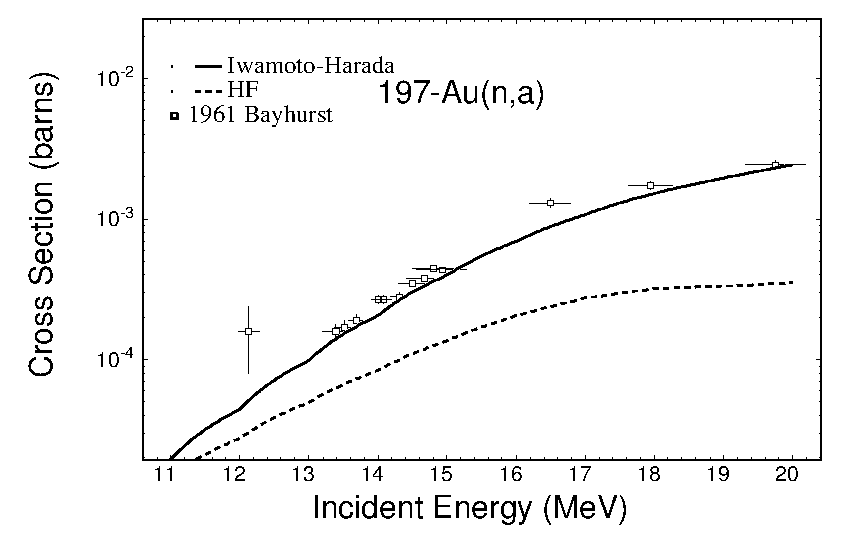
\includegraphics[width=0.7\paperwidth]{figs/hermanm1_f4}
\caption{Improvement in the description of the $^{179}$Au(n,$\protect\alpha $) reaction achieved by employing the Iwamoto-Harada model for pre-equilibrium
emission of $\protect\alpha $-particles.}
\label{goldna}
\end{figure}

\paragraph{Probability of gamma emission}

The probability of emission of gamma radiation (without spin selection
rules) is derived in a way similar to the nucleon emission probability by
applying the principle of detailed balance~\cite{Pluyko:78,Betak:79,Akkermans:85} and can be expressed as
\begin{eqnarray}
W_{\gamma }(E,n,\epsilon _{\gamma })&=&\frac{1}{\pi ^{2}\hbar ^{3}c^{2}}
\epsilon _{\gamma }^{2}\sigma _{\gamma }^{inv}(\epsilon _{\gamma })\times
\notag \\
&&\frac{\sum\limits_{k}b(k\rightarrow n,\epsilon _{\gamma })\omega
_{res}(p,h,U)}{\omega _{CN}(p,h,E)}.
\end{eqnarray}
Coefficients $b(k\rightarrow n,\epsilon _{\gamma })$ are the branching
ratios derived by Gruppelaar and Akkermans~\cite{Akkermans:85}. The inverse
reaction cross section $\sigma _{\gamma }^{inv}(\epsilon _{\gamma })$ in
the gamma channel is calculated taking into account only the contribution of
the GDR.

\paragraph{Initial and equilibrium number of excitons}

Calculations in the PCROSS module start with exciton number $n=1$, thus
taking into account the direct gamma emission. The equilibrium exciton
number is taken equal to $\sqrt{1.4 gE}$~\cite{Shang:88,Shang:89}.

\bigskip

The exciton model, as implemented in the PCROSS code, has been extensively
used in recent evaluations. Combined with the direct contributions described in
terms of the CC+DWBA models, it gave an excellent description of the forward
inelastic scattering of neutrons on $^{232}$Th in the energy range from 6.1
MeV up to 18 MeV, as can be seen in Fig. ~\ref{thspectra}.

\begin{figure}[htbp]
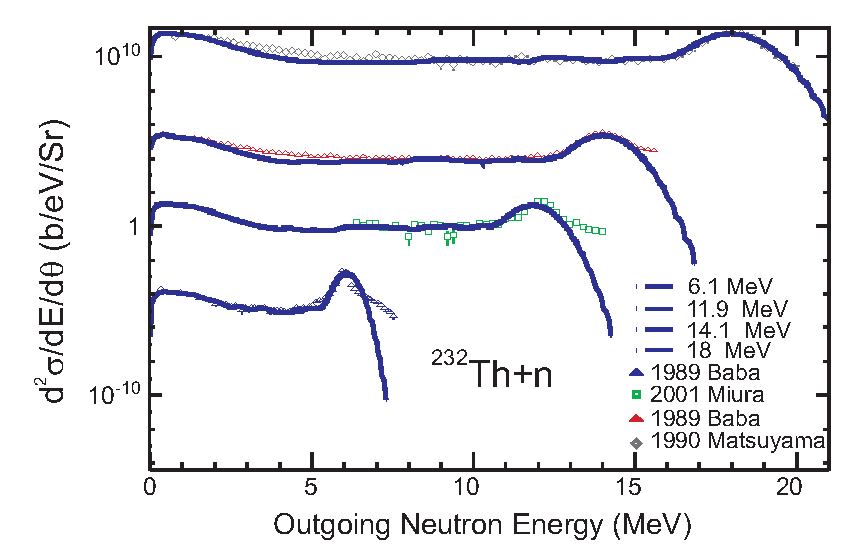
\includegraphics[width=0.7\paperwidth]{figs/thspectra}
\caption{EMPIRE calculations of the spectra of neutrons emitted at 30 degrees
for 6.1, 11.9, 14.1 and 18 MeV neutrons incident on $^{232}$Th (scaled
by 1, 10$^3$,10$^6$ and 10$^9$ respectively). Fission neutrons are not
included.}
\label{thspectra}
\end{figure}

The 18-MeV emission spectra at 60 degrees extracted from the recent IAEA
evaluation included in the ENDF/B-VII library is compared to previous
evaluations in Fig. ~\ref{thspectra18}. The advanced modeling resulted in a
dramatic improvement of the high energy part of the spectrum compared to the
previous evaluations.

\begin{figure}[htbp]
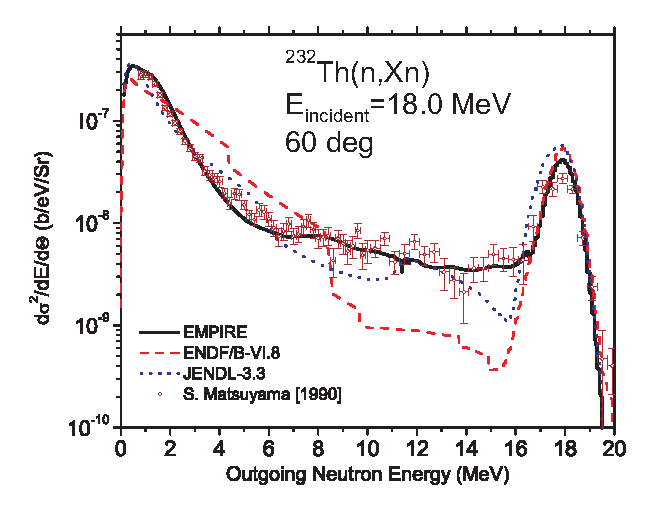
\includegraphics[width=0.7\paperwidth]{figs/thorium}
\caption{EMPIRE calculation for the neutron emission spectrum at 60 degrees
for an incident neutron energy of 18.0~MeV on $^{232}$Th, compared to
experimental data~\protect\cite{mats} and the ENDF/B-VI.8 and JENDL-3.3
libraries.}
\label{thspectra18}
\end{figure}


\section{Monte Carlo Preequilibrium (DDHMS code) \label{DDHMS}}

The Hybrid Monte-Carlo Simulation (HMS) approach to the pre-equilibrium
emission of nucleons has been formulated by M. Blann~\cite{Blann-HMS} as a
hybrid-model~\cite{hybrid,hybrid1,hybrid2,hybrid3} inspired version of the
intranuclear cascade approach. Contrary to other classical pre-equilibrium
models, this approach avoids multi-exciton level densities\index{p-h level densities}, which were shown by Bisplinghoff~\cite{Bisplinghoff} to be used inconsistently in the exciton and in the hybrid
formulations. The HMS\index{HMS} model has a number of attractive features. First of all, there
are no physical limits on the number of pre-equilibrium emissions (apart from
energy conservation). With the addition of linear momentum conservation by
M. Chadwick and P. Oblo\v{z}insk\'{y}
(DDHMS), the model provides a nearly complete set of observables.
These include cross sections for the production of residuals, light-particle
double-differential spectra and spectra of recoils. Spin and
excitation-energy dependent populations of residual nuclei can also be
obtained, an essential feature for coupling the pre-equilibrium mechanism to
the subsequent compound nucleus decay. The binding energies in the HMS\index{HMS} model are thermodynamically correct. The DDHMS model proved to
perform very well
%up to at least 250 MeV, extending energy range of the EMPIRE applicability
up to at least 250 MeV. %to the desired limit.
The calculation flow in the DDHMS model can be summarized in terms of the
following steps:

\begin{enumerate}
\item draw a collision partner for the incoming nucleon (2p-1h state created)

\item draw the energy ($\varepsilon$) of the scattered nucleon (if bound go to
step 5)

\item draw scattering angles for both particles

\item decide whether the scattered nucleon will be emitted, re-scattered or
trapped

\begin{enumerate}
\item if emitted, the appropriate cross section is augmented

\item if re-scattered, an additional particle-hole is created and one returns to
step 2

\item if trapped, go to step 5
\end{enumerate}

\item draw the excitation energy of a particle in the remaining 1p-1h
configurations (between 0 and (U-$\varepsilon$)), if unbound go to step 3, if
bound choose another existing 1p-1h pair and repeat step 5.
\end{enumerate}

All excitons (including holes) are treated on an equal footing and each of them
is given a chance to interact or be emitted with \emph{a priori} equal
probability. The cascade ends when all excitons are bound. Below, we
summarize various probability distributions which are used in concert with a
random number generator. For choosing a collision partner, it is assumed that
the unlike interaction is 3 times more probable than the like one ($\sigma_{np}=3\sigma_{nn}$). Thus, for an incident neutron we have $P_{nn}$
and $P_{np}$ for the probability of exciting neutron and proton respectively
\begin{equation}
P_{nn}=\frac{(A-Z)}{(A-Z)+3Z},  \label{Pnn}
\end{equation}

\begin{equation}
P_{np}=1-P_{nn}  \label{Pnp}
\end{equation}
and similarly for an incident proton
\begin{equation}
P_{pp}=\frac{Z}{Z+3(A-Z)},  \label{Ppp}
\end{equation}
\begin{equation}
P_{pn}=1-P_{pp}.  \label{Ppn}
\end{equation}
The energy distribution of the scattered particles $P(\varepsilon)$ is given
by the ratio of the $(n-1)-$ and $n$-exciton level densities\index{p-h level densities} $\rho_{n}$
\begin{equation}
P(\varepsilon)d\varepsilon=
\frac{\rho_{n-1}(E-\varepsilon)g}{\rho_{n}(E)}d\varepsilon,  \label{Penergy}
\end{equation}
with $n=2\, or\,3$ and
\begin{equation}
\rho_{2}(E)=\frac{g(gV)}{2}\,\,\, if\,\,\, E>V,  \label{ro2u}
\end{equation}
\begin{equation}
\rho_{2}(E)=\frac{g(gE)}{2}\,\,\, if\,\,\, E\leq V,  \label{ro2d}
\end{equation}
\begin{equation}
\rho_{3}(E)=\frac{g^{3}\left[V(2E-V)\right]}{4}\,\,\, if\,\,\, E\geq V.
\label{ro3}
\end{equation}
Here, $V$ is the potential well depth. The emission probability is calculated
as
\begin{equation}
P_{\nu}(\varepsilon-Q)=\frac{\lambda_{c}(\varepsilon-Q)}{\lambda_{c}(\varepsilon-Q)+\lambda_{+}(\varepsilon)},  \label{Pnu}
\end{equation}
with the emission rate being
\begin{equation}
\lambda_{c}(\varepsilon-Q)\sim\frac{\sigma_{\nu}(\varepsilon-Q)(
\varepsilon-Q)(2S+1)\mu_{\nu}}{g}.  \label{lambdac}
\end{equation}
Here, $\sigma_{\nu}$ is the inverse reaction cross section, $Q$ is the binding
energy, $g$ is the single-particle density, $S$ denotes nucleon spin, and $\mu_{\nu}$ stands for the reduced nucleon mass. Following the hybrid\index{HYBRID} model, $\lambda_{+}(\varepsilon)$ is calculated from the mean
free path of a nucleon in nuclear matter. The version which is actually
implemented in EMPIRE was coded by M. Chadwick and extended to
double-differential cross sections in collaboration with P. Oblo\v zinsk\' y
\cite{DDHMScode}.

Figure~\ref{pb208HMS} presents the effect of the HMS contribution on spectrum of
neutrons emitted from $^{208}$Pb bombarded with 14.6~MeV neutrons. The
compound nucleus emission underestimates
the experimental data starting at $\sim$5~MeV,
and at higher emission energies it is practically negligible. The HMS model
contribution is of the right order of magnitude to bring the
calculations into
reasonable agreement with the measurements. One notes, however, that the
model still fall short of the experimental data above 8 MeV. This
deficiency could be counteracted by adjusting the HMS input parameters (e.g.,
single-particle level densities) but such an intervention would be unphysical.
The real reason for the discrepancy is the lack of a direct reaction
contribution in the calculations reported in Fig.~\ref{pb208HMS}.
\begin{figure}[htbp]
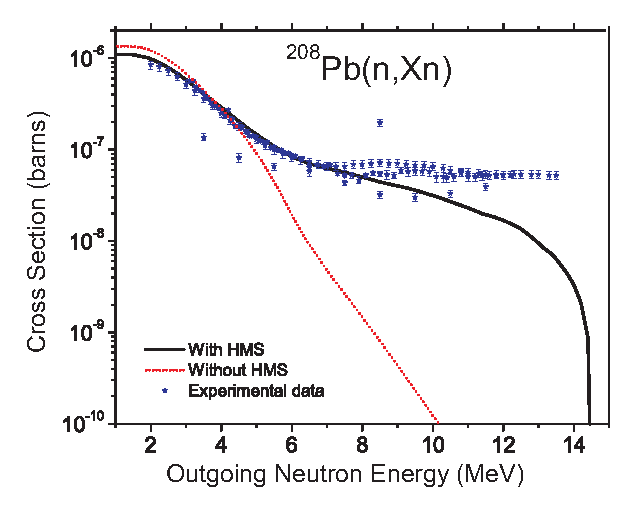
\includegraphics[width=0.7\paperwidth]{figs/pb208}
\caption{Contribution of the pre-equilibrium processes, modeled using Monte Carlo
simulation, to neutron spectrum from the $^{208}$Pb(n,xn) reaction at 14.6~MeV.}
\label{pb208HMS}
\end{figure}

\section{Compatibility of preequilibrium models }

Possible inclusions of different preequilibrium models in a single
calculation run rises a problem of double-counting. The current version
of EMPIRE has 4 modules for preequilibrium decay: MSD\index{MSD},
MSC\index{MSC},  HMS\index{HMS} and PCROSS\index{PCROSS}.
While MSD and MSC describe different reaction mechanisms and are complementary,
neither of them is compatible with HMS or PCROSS. Therefore,
neither of the latter two can be used together with MSD or MSC in
the same exit channel. Also HMS and PCROSS mutually exclude
each other. However, these models can be combined if used in different
exit channels, e.g., neutron inelastic scattering may be calculated
using MSD\&MSC while the emission of protons can be treated within
the exciton model using PCROSS. We also note that summing $\gamma$-emission
spectra from more than one of the two possible mechanisms (MSC\index{MSC}
(GST=1 option) or PCROSS) would be obvious multiple-counting and must be avoided.

An additional complication is introduced by the possibility of using
ECIS06\index{ECIS} or OPTMAN code, which calculate Coupled-Channel\index{Coupled-Channels}
contributions to the collective discrete levels. In general, these
contributions are so strong that adding those provided by the exciton
model leave the results practically unchanged. Thus, ECIS06/OPTMAN can be
considered compatible with HMS\index{HMS} since the latter does not include
collective excitations. By the same token ECIS06/OPTMAN codes are not
compatible with MSD\index{MSD} as both include collectivity of discrete
levels. However, ECIS06/OPTMAN and MSD can be combined providing that only
the continuum contribution from the MSD is retained.

To avoid double-counting when combining different models EMPIRE applies
the following priorities:

\begin{description}
\item [{ECIS06\index{ECIS} or OPTMAN}] provides inelastic scattering to collective
levels independently of the settings for the remaining models. 
\item [{MSD\index{MSD}}] provides inelastic continuum independently of
other settings. Inelastic to the discrete levels is suppressed if
ECIS06 is active. Note the provision for the second-chance preequilibrium
emission after MSD.
\item [{MSC\index{MSC}}] results are taken for the inelastic to the continuum.
Charge-exchange to the continuum is accepted if not suppressed by
use of HMS\index{HMS} or PCROSS\index{PCROSS}. 
\item [{HMS\index{HMS}}] provides inelastic and charge-exchange to the
continuum and to discrete levels if MSD\index{MSD} and MSC\index{MSC}
are not active. Otherwise only the charge-exchange contribution is
used. Suppresses PCROSS results for particle emission
if such was calculated. HMS does not provide $\gamma$-rays, thus
PCROSS or MSC results are adopted. 
\item [{PCROSS\index{PCROSS}}] provides inelastic and charge-exchange
to the continuum if these are not provided by any of the above listed
models. Provides $\gamma$-emission if not suppressed by $\gamma$-emission
from MSC. Provides preequilibrium emission of clusters independently
of settings for other models.
\end{description}
This scheme allows the user to activate any combination of reaction
mechanisms while the code ensures the internal consistency of calculations.
Overlapping contributions from various models are summed up and the
Compound Nucleus contribution is added in all cases. A concise summary
explaining use of the models is printed as a table at the beginning
of the lengthy output \emph{{*}.lst}. An example is reproduced below:

\hfill{}

\texttt{Use of direct and preequilibrium models }

\texttt{-{}-{}-{}-{}-{}-{}-{}-{}-{}-{}-{}-{}-{}-{}-{}-{}-{}-{}-{}-{}-{}-{}-{}-{}-{}-{}-{}-{}-{}-{}-{}-{}-{}-{}-{}-{}-{}- }

\texttt{Exit channel ECIS MSD MSC HMS PCROSS }

\texttt{neut. disc. ~0~~~ 1~~ 0~~~0~~~~0 }

\texttt{neut. cont. ~0~~~ 1~~ 1~~ 0~~~~0}

\texttt{prot. disc. ~0~~~ 0~~ 0~~ 0~~~~0}

\texttt{prot. cont. ~0~~~ 0~~ 0~~ 0~~~~1}

\texttt{gammas ~~~~~~~~0~~~ 0~~ 0~~ 0~~~~1}

\texttt{alpha cont.~~ 0~~~ 0~~ 0~~ 0~~~~1}

\hfill{}

\noindent 1 indicates that the contribution of the model is included,
and 0 means that it is not calculated or ignored. In the above example,
MSD\index{MSD}, MSC\index{MSC} and PCROSS\index{PCROSS}
were invoked, and priority rules caused PCROSS neutron contribution
to be suppressed  leaving emission of protons and
clusters.

Selecting DIRECT =1 (or 2 or 3), MSD=1, MSC=1, PCROSS=1.5 is supposed
to give the best results at low incident nucleon energies (say up to 50 MeV).
At higher incident energies the preference should be given to the
HMS\index{HMS} model, which is the only one that accounts for the multiple preequilibrium
emission. When selecting appropriate models the user should take into
account that not all of them provide the same set of observables.
For example, preequilibrium $\gamma$-emission can be obtained from PCROSS or MSC\index{MSC}
but not from HMS. 

%
%
%
%
%
%
%The Hybrid Monte-Carlo Simulation (HMS) approach to the preequilibrium
%emission of nucleons is the third precompound model included in EMPIRE
%(the other two are MSD\index{MSD}\&MSC\index{MSC} and the exciton
%model (PCROSS\index{PCROSS})). The original HMS\index{HMS} model has
%been formulated by M. Blann \cite{Blann-HMS} as a hybrid model \cite{hybrid,hybrid1,hybrid2,hybrid3}
%inspired version of the intranuclear cascade approach. Contrary to
%other classical preequilibrium models, this approach avoids multi-exciton
%level densities\index{p-h level densities}, which were shown by Bisplinghoff
%\cite{Bisplinghoff} to be used inconsistently in the exciton and
%in the hybrid formulations. The HMS\index{HMS} model has a number
%of attractive features. First of all, there are no physical limits
%on a number of preequilibrium emissions (apart from energy conservation).
%With the addition of linear momentum conservation by M.Chadwick and
%P. Oblo\v zinsk\' y (DDHMS), the model provides a nearly complete
%set of observables. These include cross sections for the production
%of residuals, light-particle double-differential spectra and spectra
%of recoils. Spin and excitation-energy dependent populations of residual
%nuclei can also be obtained, an essential feature for coupling the
%preequilibrium mechanism to the subsequent Compound Nucleus decay.
%The binding energies in the HMS\index{HMS} model are thermodynamically
%correct. This is a clear improvement over the intranuclear cascade
%model, although exact account, typical of the Compound Nucleus model,
%is still out of reach. The DDHMS model proved to perform very well
%up to at least 250 MeV, extending energy range of the EMPIRE applicability
%to the desired limit.
%
%The calculation flow in the DDHMS model can be summarized in terms
%of the following steps:
%
%\begin{enumerate}
%\item draw collision partner for the incoming nucleon (2p-1h state created)
%\item draw energy ($\varepsilon$) of the scattered nucleon (if bound go
%to step 5)
%\item draw scattering angles for both particles
%\item decide whether the scattered nucleon will be emitted, re-scattered
%or trapped
%
%\begin{enumerate}
%\item if emitted appropriate cross section is augmented
%\item if re-scatters additional particle-hole is created and we return to
%step 2
%\item if trapped, go to step 5
%\end{enumerate}
%\item draw excitation energy of a particle in the remaining 1p-1h configuration
%(between 0$\div(U-\varepsilon)$), if unbound go to step 3, if bound
%choose another existing 1p-1h pair and repeat step 5.
%\end{enumerate}
%All excitons (including holes) are treated on equal footing and each
%of them is given a chance to interact or being emitted with \emph{a
%priori} equal probability. The cascade ends when all excitons are
%bound. Below, we summarize various probability distributions which
%are used in concert with a random number generator. 
%
%For choosing a collision partner it is assumed that the unlike interaction
%is 3 times more probable than the like one ($\sigma_{np}=3\sigma_{nn}$).
%Thus, for the incident neutron we have $P_{nn}$ and $P_{np}$ for
%the probability of exciting neutron and proton respectively
%
%\begin{equation}
%P_{nn}=\frac{(A-Z)}{(A-Z)+3Z},\label{Pnn}\end{equation}
% 
%
%\begin{equation}
%P_{np}=1-P_{nn}\label{Pnp}\end{equation}
% and similarly for the incident proton
%
%\begin{equation}
%P_{pp}=\frac{Z}{Z+3(A-Z)},\label{Ppp}\end{equation}
%\begin{equation}
%P_{pn}=1-P_{pp}.\label{Ppn}\end{equation}
%The energy distribution of the scattered particles $P(\varepsilon)$
%is given by the ratio of the $(n-1)-$ and $n$-exciton level densities\index{p-h level densities}
%$\rho_{n}$
%
%\begin{equation}
%P(\varepsilon)d\varepsilon=\frac{\rho_{n-1}(E-\varepsilon)g}{\rho_{n}(E)}d\varepsilon,\label{Penergy}\end{equation}
%with $n=2\, or\,3$ and\begin{equation}
%\rho_{2}(E)=\frac{g(gV)}{2}\,\,\, if\,\,\, E>V,\label{ro2u}\end{equation}
%\begin{equation}
%\rho_{2}(E)=\frac{g(gE)}{2}\,\,\, if\,\,\, E\leq V,\label{ro2d}\end{equation}
%\begin{equation}
%\rho_{3}(E)=\frac{g^{3}\left[V(2E-V)\right]}{4}\,\,\, if\,\,\, E\geq V.\label{ro3}\end{equation}
% Here, $V$ is a potential well depth. The emission probability is
%calculated as 
%
%\begin{equation}
%P_{\nu}(\varepsilon-Q)=\frac{\lambda_{c}(\varepsilon-Q)}{\lambda_{c}(\varepsilon-Q)+\lambda_{+}(\varepsilon)},\label{Pnu}\end{equation}
%with the emission rate being
%
%\begin{equation}
%\lambda_{c}(\varepsilon-Q)\sim\frac{\sigma_{\nu}(\varepsilon-Q)(\varepsilon-Q)(2S+1)\mu_{\nu}}{g}.\label{lambdac}\end{equation}
%$\sigma_{\nu}$ is an inverse reaction cross section, $Q$ is a binding
%energy, $g$ is a single particle density, $S$ denotes nucleon spin,
%and $\mu_{\nu}$ stands for the reduced nucleon mass. Following the
%hybrid\index{HYBRID} model, $\lambda_{+}(\varepsilon)$ is calculated
%from the mean free path of a nucleon in nuclear matter.
%
%The version which is actually implemented in EMPIRE has been coded
%by M. Chadwick and extended to double-differential cross sections
%in collaboration with P. Oblo\v zinsk\' y \cite{DDHMScode}.

\chapter{Compound nucleus model}

\section{Compound Nucleus}

The statistical model used in the EMPIRE is an advanced implementation
of the Hauser-Feshbach\index{Hauser-Feshbach} theory. The exact angular
momentum and parity coupling is observed. The emission of neutrons,
protons, $\alpha$-particles, deuterons, tritons, and He-3 is taken into 
account along with the competing fission channel. The full $\gamma$-cascade
in the residual nuclei is considered. 

To account for the correlation between incident and exit channels in
elastic scattering (width fluctuation correction)the model proposed by 
Hofmann, Richert, Tepel and Weidenmueller (HRTW)~\cite{HRTW} is used. 
This model is briefly reviewed in the next subsection.
Particular attention is dedicated to the determination of the level 
densities\index{level densities}, which can be calculated in the 
non-adiabatic approach allowing for the rotational and vibrational 
enhancements (see Section~\ref{NLD}). 

In the Hauser-Feshbach model the $(a,b)$ reaction cross section
is written as:
\begin{equation}
\sigma_{a,b}(E)=\sum_{J\pi}\sigma_{a}^{CN}(E,J\pi)P_{b}(E,J\pi)
\label{Hauser}
\end{equation}
where $\sigma_{a}^{CN}(E,J\pi)$ is the cross section of the compound nucleus formation  
in a state of spin and parity $J\pi$ associated to the incident channel $a$ 
and $P_{b}(E,J\pi)$ represents the decay probability of the compound nucleus with
the excitation energy $E_x$ in $b$ channel.
The decay probability is defined in terms of transmission coefficients 
\begin{equation}
P_{b}(E,J\pi)=\frac{T_{b}(E_x,J\pi)}{\sum_{c}T_{c}(E_x,J\pi)}
\end{equation}
associated to the reaction channels which might be particles emission, photon emission or fission.
\\
The transmission coefficient for the $p$ particle emission has the expression

\begin{equation}
T_p(E,J\pi)=\sum_{I=|J-j|}^{I=J+j}\int_0^{E_x-B_p}\sum_{lj}T_{p,lj}(E_x-B_p+\varepsilon)
            \rho(\varepsilon,I\pi_I)\delta(\pi\pi_I,(-1)^l) d\varepsilon
\end{equation}
where $B_{p}$ is the separation energy of particle $p$ in
the compound nucleus, $\rho(\varepsilon,I\pi_I)$ is the density \index{level density})
of levels in the residual nucleus with the spin and parity 
$I,\pi_I$ and the excitation energy $\varepsilon$,
and $T_{p,lj}$ stands for the transmission coefficient (discussed in Chapter ...)
having channel energy $E_x-B_{p}-\varepsilon$ and
orbital angular momentum $l$, which together with the particle spin
$s$ couples to the channel angular momentum $j$ used to select in the residual nucleus spins $I$
populated for a given compound nucleus spin $J$. The factor $\delta(\pi\pi_I,(-1)^l)$ stands
for parity conservation.
For the discrete
levels (characterized by the energy $E_{i}$, spin $I_{i}$, and parity
$\pi_{I_i}$) the level density $\rho(\varepsilon,I,\pi_I)$ reduces to 
$\delta(\varepsilon-E_{i})\delta(I,I_{i})\delta(\pi_I,\pi_{I_i})$.
A similar expression is used for the gamma-decay coefficient
\begin{equation}
T_{\gamma}(E_x,J\pi)=\sum_{XL}\sum_{J'=|J-L|}^{|J+L|}\int_0^{E_x}f_{Xl}(\varepsilon_{\gamma})
\rho(E_x-\varepsilon_{\gamma},J',\pi')\delta(\pi\pi',(-1)^L)d\varepsilon_{\gamma}
\end{equation}
where $XL$ represents the photon type and multipole, $J'\pi'$ are the spin and parity of
the final states and $f_{XL}(\varepsilon_{\gamma})$ is the $\gamma$-ray strength function
discussed in more detail in Section \ref{gamma-decay}.
The fission coefficients are presented in Section \ref{fission}. 

It should be mentioned that the above equations also hold for secondary CNs that are formed due 
to subsequent emissions of particles. The only difference is that while the first
CN is initially excited to the unique (incident channel compatible)
energy, the secondary CNs are created with excitation energies which
spread over the available energy interval.


%%%%%%%%%%%%%%%%%%%%%%%%%%%%%%%%%%%%%%%%%%%%%%%%%%%%%%%%%%%%%%%%%%%%%%%%%%%%%%%%%%%%%%%%%%%%%%%%%%%%%%%%%%%%%%%%%%
\subsection{Width fluctuation correction}
To account for the correlation between incident and exit channels in
elastic scattering we use model proposed by Hofmann, Richert, Tepel
and Weidenmueller (HRTW)~\cite{HRTW}. In the case of no direct reaction
contribution, the averaged $S$-matrix element connecting channels $a$ and
$b$ can be written as
\begin{equation}
<S>_{ab}=\delta_{ab}e^{i\varsigma_{ab}}(1-T_{a})^{1/2},
\label{Sab}
\end{equation}
\noindent where
\begin{equation}
T_{a}=1-|<S>_{aa}|^{2}
\label{Ta}
\end{equation}
is an optical model transmission coefficient. The HRTW model assumes
that the Compound Nucleus (CN) cross sections factorize and
can be expressed through a product of the channel dependent quantities
$\xi$. This would be the famous Bohr's assumption if not for the
elastic enhancement factor $W_{a}$, which has been introduced by
HRTW in order to account for the elastic channel correlation
\begin{equation}
<\sigma_{ab}^{fl}>=\xi_{a}\xi_{b}\quad a\neq b\qquad and\qquad<\sigma_{a}^{fl}>=W_{a}\xi_{a}^{2}.
\label{Sig-fluc}
\end{equation}
 Setting
\begin{equation}
\xi_{a}=\frac{V_{a}}{\sqrt{\sum_{c}V_{c}}}
\label{ksi}
\end{equation}
we get for the CN cross section
\begin{equation}
\sigma_{ab}^{CN}\equiv<\sigma_{ab}^{fl}>=V_{a}V_{b}\left(\sum_{c}V_{c}\right)^{-1}\left[1+\delta_{ab}\left(W_{a}-1\right)\right].
\label{Sig-flucV}
\end{equation}
Taking into account that the incoming flux has to be conserved (unitary
condition) we find the relation between $V$s, the elastic enhancement
factor ($W_{a}$), and the transmission coefficient ($T_{a}$)
\begin{equation}
V_{a}=T_{a}\left[1+\frac{V_{a}}{\left(\sum_{c}V_{c}\right)}\left(W_{a}-1\right)\right]^{-1}.
\label{Va}
\end{equation}
This equation can be solved for $V_{a}$ by iteration once all $W_{a}$
are known. The current version of EMPIRE uses $W_{a}$ derived from
the analysis of numerically generated sets of $S$-matrices~\cite{HHM}.
The resulting formula for the elastic enhancement factor is
\begin{equation}
W_{a}=1+2\left[1+T_{a}^{F}\right]^{-1}+87\left(\frac{T_{a}-T_{ave}}{\sum_{c}T_{c}}\right)^{2}\left(\frac{T_{a}}{\sum_{c}T_{c}}\right)^{5},
\label{Wa}
\end{equation}
with
\begin{equation}
F=4\frac{T_{ave}}{\sum_{c}T_{c}}\left(1+\frac{T_{a}}{\sum_{c}T_{c}}\right)\left(1+3\frac{T_{ave}}{\sum_{c}T_{c}}\right)^{-1},
\label{Wa-F}
\end{equation}
which completes formulation of the model.

%==========================================================================
\section{Level densities}
%==========================================================================
\label{NLD}
In EMPIRE the level densities \index{level densities} are described by several models 
with the corresponding parametrizations.
Three of them are phenomenological (Gilbert-Cameron Model (GCM), Generalized Superfluid Model (GSM),
Enhanced Generalized Superfluid Model (EGSM)) and one is based on Hartree-Fock-Bogoliubov 
microscopic model (HFBM). All of them are included also in RIPL. Another common feature is 
that they are parametrized or normalized to reproduce the average parameters of the neutron resonances
and the data on the cumulative number of low-lying nuclear levels.
Choice of the proper representation depends on a case being considered.

The best known and used level density analytical expression was derived within Fermi-Gas Model (FGM), therefore
the basic relations of FGM are presented in subsection \ref{FG}. The following subsections are dedicated to
each of the above four models.

%*************************************************************
\subsection{Basic relations of Fermi-Gas Model}
%*************************************************************
\label{FG}

The density of intrinsic levels with spin $J$, parity $\pi$ and excitation energy $E_x$ is
factorised in terms of state density and spin and parity dependence as 
\begin{equation}
\rho(E_x,J,\pi)=\rho(E_x)\rho(J,\pi).
\label{ld-FG1}
\end{equation}
The energy dependence reads 
\begin{equation}
\rho(E_x)=\frac{\exp{S}}{\sqrt{Det}}
\label{ld-rhoE}
\end{equation}
where $S$ is the entropy and $Det$ is defined by Eq.\ref{ld-stat}. 
\\
The spin and parity dependence is given by
\begin{equation}
\rho(J,\pi)=\frac{1}{2}\frac{(2J+1)}{\sqrt{8\pi\sigma^3}}\exp\left[-\frac{(J+1/2)^2}{2\sigma^2}  \right]
\label{ld-rhoJ}
\end{equation}
where $\sigma^2$ is the spin cut-off parameter and equal parity distribution is assumed.
\\
For the Fermi-Gas model the state equations determining the dependence of the excitation energy, entropy
and other thermodinamic functions of a nucleus on its temperature $T$ are
\begin{equation}
E_x=aT^2;\quad S=2aT;\quad \sigma^2=\Im T;\quad Det=144a^3T^5/\pi
\label{ld-stat}
\end{equation}
where $a$ is the level density parameter and $\Im$ is the nuclear moment of inertia. 
\\
To account for the odd-even effects in nuclei, the excitation energy is replaced in calculations with the
effective energy $U$
\begin{equation}
U=E_x-\Delta
\label{ld-u}
\end{equation}
where $\Delta$ is equal or closely related to the pairing energy.

Introducing Eqs.\ref{ld-stat}, \ref{ld-u} in Eq.\ref{ld-rhoE} the well known expression for the state 
density is obtained 
\begin{equation}
\rho^{FG}(E_x)=\frac{\sqrt{\pi}}{12a^{1/4}U^{5/4}}\exp{(2\sqrt{aU})}
\label{ld-rhoE1}
\end{equation}
and the level density becomes
\begin{equation}
\rho^{FG}(E_x,J,\pi)=\frac{2J+1}{48\sqrt{2}\sigma^{3/2}a^{1/4}U^{5/4}}\exp{\left[2\sqrt{aU}-
\frac{(J+1/2)^2}{2\sigma^2}\right]}.
\label{ld-rhoEjp1}
\end{equation}
These equations show that nuclear level densities in Fermi-Gas model depend on three parameters:
$a$, $\sigma$ and $\Delta$. Some general features about the energy and mass dependence of $a$ parameter
are outlined here, more details about these parameters being discussed
in the subsections on various specific level density models.

The correlation between the $a$-parameter values  deduced from the neutron resonance spacing and the 
shell correction and the fade-out of the shell effects with increasing the excitation energy imply 
energy dependence of the $a$ parameter.
The general form of this dependence was proposed by Ignatyuk~\cite{ignaa}
\begin{equation}
a(E_x)=\widetilde{a}\left[1+f(U)\frac{\delta W}{U}\right],
\label{apiccoloGC}
\end{equation}
\noindent where $\delta W$ is the shell correction, $\widetilde{a}$ is the
asymptotic value of the $a$-parameter and
\begin{equation}
f(U)=1-\exp(-\gamma U)
\label{shellGC}
\end{equation}
with $\gamma$ being the shell effects damping parameter.


%****************************************************************
\subsection{Gilbert-Cameron Model}
%****************************************************************
\label{GCM}
The Gilbert-Cameron approach \cite{gc} splits excitation energy in
two regions. Different functional forms of level densities\index{level densities}
are applied in each of them. The constant temperature formula applies at low 
excitation energies (below the matching point $U_{x}$) and the Fermi Gas formula 
is used above $U_{x}$ 
\begin{equation}
\rho^{GC}(E_x)=\left\{\begin{array}{l}{\rho^{CT}(E_x)\quad {E_x \leq U_x}}\\ 
\rho^{FG}(E_x)\quad E_x > U_x\end{array}\right ..
\label{ld-gc}
\end{equation}
The constant temperature level density reads
\begin{equation}
\rho^{GC}(E_x,J,\pi)=\rho^{GC}(E_x)\rho(J,\pi)
\label{ld-gc1}
\end{equation}
with $\rho(J,\pi)$ from Eq.\ref{ld-rhoJ}.
\\
In the constant temperature region the state density  is
\begin{equation}
\rho^{CT}(E_x)=\frac{1}{T}\exp\left(\frac{E_x-E_0}{T}\right)
\label{ld-ct}
\end{equation}
where $T$ is the nuclear temperature and $E_0$ is a free parameter.
The three model parameters, $T,\, U_{x},$ and $E_{0}$ are determined
by the requirement that the level density and its derivative are continuous
at the matching point $U_{x}$, and by fitting cumulative number of
discrete levels with the integral of Eq. \ref{ld-gc}. 

%The first of the conditions implies
%\begin{equation}
%\frac{1}{T}=\sqrt{a/U_{x}}-\frac{3}{2U_{x}}.
%\label{condUT}
%\end{equation}

The Fermi Gas state density $\rho^{FG}(E_x)$ is given by Eq.\ref{ld-rhoE1} where the effective
excitation energy is $U=E_x-\Delta$. The pairing energy is calculated as
\begin{equation}
\Delta=n\frac{12}{\sqrt{A}}
\label{del}
\end{equation}
where $n$=0,1 and 2 for odd-odd, odd-A and even-even nuclei respectively.

The calculation can be performed using constant or energy dependent $a$-parameter.
The constant $a$-parameter is read from input (GCROA).
Alternatively can be used the general form given by Eq. \ref{apiccoloGC} which
accounts for the shell effects, and their fade-out
with increasing energy.
The three relevant systematics available in EMPIRE are:
\begin{description}
\item[Ignatyuk~\emph{et al.}~\cite{ignaa}]: $\widetilde{a}=0.154A+6.3\cdot10^{-5}A^{2}$
and $\gamma=-0.054$
\item[Arthur~\cite{arthura}]: $\widetilde{a}=0.1375A-8.36\cdot10^{-5}A^{2}$
and $\gamma=-0.054$
\item[Iljinov~\emph{et al.}~\cite{Mebel}]: $\widetilde{a}=0.114A+9.80\cdot10^{-2}A^{2/3}$
and $\gamma=-0.051$
\end{description}


The spin cut-off factor $\sigma(E_x)$ is given by
\begin{equation}
\sigma^{2}(E_x)=0.146A^{2/3}\sqrt{aU}.
\label{sigld}
\end{equation}


We stress that Gilbert-Cameron approach does not account explicitly
for the collective enhancements of the level densities\index{level densities}.
These are included implicitly in the $\widetilde{a}$ when fitting
neutron resonance spacings. Such an approach leads to the over-estimation
of the level densities above, say, 20 MeV.

For the nucleon induced reactions, with CN excited up to about 20
MeV, the Gilbert-Cameron approach is recommended. It assures an
accurate description of level densities in the energy range up to
the neutron binding energy. The collective effects are included in
the level density parameter $a$, providing reasonable estimate of
the level densities as long as damping of the collective effects is
irrelevant. The relatively low angular momentum introduced by the
incident projectile justifies neglect of dynamical effects.

%****************************************************************
\subsection{Generalized Superfluid Model}
%****************************************************************

The phenomenological version of the Generalized Superfluid Model (GSM) is 
characterized by a phase 
transition from superfluid behaviour at low energy~\cite{ignaa,83I}, 
where pairing correlations strongly influence the
level density, to a high energy region which is described by
the FGM. Thus, the GSM resembles the GC to the extent that the model
distinguishes between a low energy and a high energy region, although for
the GSM this distinction follows naturally from the theory and does not
depend on specific discrete levels that determine a matching energy.

The influence of the superconducting pairing correlations on nuclear
properties can be characterized by the value of the correlation function $\Delta_0$, which determines directly the even-odd differences in the nuclear
binding energies and the energy gap of $2\Delta_0$ in the spectrum of
quasi-particle excitations in even-even nuclei. The critical temperature $T_{c}$ of the phase transition from a superfluid to a normal state is
connected with the correlation function through the relation
\begin{equation}
T_{c} = 0.567 \Delta_0~.  \label{ig523}
\end{equation}
The excitation energy corresponding to the critical temperature, i.e.,
the critical energy $U_c$, may be expressed as
\begin{equation}
U_c=a_c T_c^2 \, + \, E_{cond}~,  \label{Uc}
\end{equation}
\noindent where $E_{cond}$ is the condensation energy for the even-even nucleus
that determines a reduction of the nuclear ground state energy due to the pairing correlations
\begin{equation}
E_{cond} = \frac{3}{2\pi^2} a_c \Delta_0^2~.  \label{cond}
\end{equation}

The critical value of the determinant $Det_{c}$, and the
critical entropy $S_{c}$ are defined by the following expressions
\begin{equation}
Det_{c}=\left(\frac{12}{\sqrt{\pi}}\right)^{2}a_{c}^{3}T_{c}^{5}\,,\label{Detcrt}
\end{equation}
\begin{equation}
S_{c}=2a_{c}T_{c}\,.\label{Scrt}
\end{equation}
The parallel and perpendicular moments of inertia at the critica energy are calculated in terms of
deformation as
\begin{equation}
\Im_{\parallel c}=\frac{6}{\pi^2} a_c <{m^2}>(1-\frac{2}{3}\beta_2)
\end{equation}

\begin{equation}
\Im_{\perp c}=\frac{6}{\pi^2} a_c <{m^2}>(1+\frac{1}{3}\beta_2)
\end{equation}
where $a_c$ is the critical value of the level density $a$-parameter and $<m^2>$ is the average value 
of the square of the projection of angular momentum for single-particle states on the Fermi surface 
parametrized as $<m^2>=0.24 A^{2/3}$.

One can notice that all the critical values described above are expressed in terms 
of the correlation function $\Delta_0$ estimated as $\Delta_0=12/\sqrt{A}$ and 
the critical $a_c$-parameter determined by the iteration procedure
\begin{equation}
a_{c}^{(0)}=\widetilde{a}\left(1+\gamma\delta_{W}\right)\label{ait0}
\end{equation}
\begin{equation}
U^{(n)}=a_{c}^{(n)}T_{c}^{2}\label{Uit}
\end{equation}
\begin{equation}
a_{c}^{(n+1)}=\widetilde{a}\left[1+\frac{\delta_{W}}{U^{(n)}}\left(1-\exp\left(-\gamma U^{(n)}\right)\right)\right]\,.\label{ait}
\end{equation}
where $\widetilde{a}$ is the asymptotic value of the level density parameter.
Eqs. \ref{Uit} and \ref{ait} are iterated until the condition
\begin{equation}
\frac{\left|a^{(n+1)}-a^{(n)}\right|}{a^{(n+1)}}<0.001\label{itercond}
\end{equation}
is fulfilled. 

Both below and above the critical energy the quasi-particle level density has the same expression given
by Eqs. \ref{ld-FG1},\ref{ld-rhoE}, \ref{ld-rhoJ}
\begin{equation}
\rho_{qp}(E_x,J,\pi)=\frac{\exp{S}}{\sqrt{Det}}
\frac{1}{2}\frac{(2J+1)}{\sqrt{8\pi\sigma^3_{eff}}}\exp\left[-\frac{(J+1/2)^2}{2\sigma_{eff}^2}  \right]
\label{ld-gsm}
\end{equation}
but with the thermodinamic quantities defined differently.

The calculations are performed for the effective excitation energy 
\begin{equation}
U=E_x+n\Delta_0+\delta_{shift}
\end{equation}
where $\Delta_0=12/\sqrt{A}$ and $n$=0, 1 and 2 for even-even, odd-A and odd-odd nuclei, respectively.
The energy shift $\delta_{shift}$ was introduced to
account for possible shortcomings of the global systematics.

At effective excitation energies below $U_{c}$, in the energy range
where the superconductivity model BCS\index{BCS}  \cite{igna} applies, the function $\varphi$ is introduced 
\begin{equation}
\varphi=\sqrt{1-U/U_{c}}\,,\label{fiign}
\end{equation}
which allows to express all thermodynamical quantities in terms of their critical values.
\\
Above $U_c$ the condensation energy is subtracted from the effective excitation energy 

\begin{equation}
U^{*}=U-E_{cond}.
\end{equation}
The quantities entering GSM formulation are calculated with the following
expressions

\begin{equation}
a=\left\{\begin{array}{lr}
a_{c} & U\leq U_{c}\\
\tilde a  [1+\delta W (1-\exp(-\gamma U^*))/U^*]& U>U_{c} 
\end{array}\right .
\label{a}
\end{equation}


\begin{equation}
T=\left\{\begin{array}{lr}
2\varphi T_{c}/\ln \frac{\varphi +1}{1-\varphi} & U\leq U_{c}\\ 
\sqrt{\frac{U^{*}}{a}}& U> U_{c}
\end{array}\right .
\end{equation}

\begin{equation}
S=\left\{\begin{array}{lr}
S_{c}T_c(1-\varphi^{2})/T & U\leq U_{c}\\ 
2aT & U> U_{c}
\end{array}\right .
\end{equation}

\begin{equation}
{\rm Det}=\left\{\begin{array}{lr}
{\rm Det}_{c}(1-\varphi^2)(1+\varphi^2)^2 & U\leq U_{c}\\ 
144 a^3T^5/\pi & U> U_{c}
\end{array}\right .
\end{equation}

\begin{equation}
\Im_{\parallel}=\left\{\begin{array}{lr}
\Im_{\parallel c}T_{c}(1-\varphi^{2})/T& U\leq U_{c}\\ 
\Im_{\parallel c}  & U> U_{c}
\end{array}\right .
\end{equation}



\begin{equation}
\Im_{\perp}=\left\{\begin{array}{lr}
\frac{1}{3}\Im_{\perp}+\frac{2}{3}\Im_{\perp}T_{crt}(1-\varphi^{2})/T& U\leq U_{c}\\ 
\Im_{\perp c}  & U> U_{c}
\end{array}\right .
\end{equation}
\\
Squares of the effective spin cut-off parameters are defined as
\begin{equation}
\begin{array}{ll}
\sigma_{eff}^{2}=\Im_{\parallel}T & \,\,\, for\,\,\beta_{2}<0.005\,,\\
\sigma_{eff}^{2}=\left(\Im_{\parallel}\right)^{1/3}\left(\Im_{\perp}^{BCS}\right)^{2/3}T & \,\,\, for\,\,\beta_{2}>0.005\,,\end{array}\label{sigeffign}
\end{equation}
with $\beta_{2}$ being ground state deformation. 

The final expression of the GSM level density is obtained by adding to Eq. \ref{ld-gsm} in an adiabatic mode
the rotational and vibrational enhancements ($K_{rot}$, $K_{vib}$) and their damping with increasing energy 
($Q_{rot}$, $Q_{vib}$) that results in
\begin{equation}
\rho(E_x,J,\pi)=\rho_{qp}(E_x,J,\pi)K_{rot}Q_{rot}K_{vib}Q_{vib}\,.\label{roBCScol}
\end{equation}
\\ 
{\bf Rotational enhancement.} In the adiabatic approximation, the rotational enhancement of the level
density depends on the nuclear shape symmetry and can be written as \cite{BM}
\begin{equation}
K_{rot} = \left\{
\begin{array}{ll}
1 & \mathrm{for~spherical~nuclei ,} \\
{\Im}_{\perp}T & \text{for~deformed~nuclei .}
\end{array}
\right.  \label{Krot}
\end{equation}
This formula is valid if the mirror and axial symmetry
of a deformed nuclei is assumed. The most stable nuclei of the rare-earth elements
 ($150 \le A\le 190$) and the actinides $A\ge 230$ are of this shape. For non-axial
forms the rotational enhancement of the level density becomes greater \cite{BM} (see fission level densities in Section~\ref{fission}).
\\
Over the previous twenty years, some microscopic models have been developed
to consider collective effects in highly excited nuclei. The results of all
these models demonstrate the damping of level density enhancement factors
with increase of excitation energy. On the basis of the level density
calculations within the SU(3) model (oscillator mean field with 
quadrupole-quadrupole interaction between particles), Hansen and Jensen \cite{83H} obtained the following empirical function for the rotational damping factor
\\
\begin{equation}
Q_{rot}=q_r\left[1-\frac{1}{{\Im}_{\perp}T}\right]+\frac{1}{{\Im}_{\perp}T}
\label{ig5301}
\end{equation}
with
\begin{equation}
q_{r}=\frac{1}{1+\exp [(U-U_{r})/d_{r}]}~,
\label{ig530}
\end{equation}
Originally it was supposed that the damping parameters could strongly depend upon
nuclear deformations. However, the analysis of heavy nuclei fissilities
\cite{90R,98J} shows that damping is independent of deformation with
the corresponding parameters $U_{r}=40$ MeV and $d_{r}=10$ MeV. Of course,
uncertainties of these parameters are rather large and additional
confirmations are required. Nevertheless, it seems that the damping of the
rotational enhancement is comparable with the damping of the shell effects
in magic nuclei.
 The two terms
in Eq. \ref{Qrot} ensure that $Q_{rot}=0$ at $U=0$ and tends to
1 for $U\rightarrow\infty$. We note that $1/\Im_{\bot}t$
is approximately equal to the rotational enhancement and therefore
multiplication of the level densities\index{level densities} by Eq.
\ref{damp} actually removes rotational enhancement when $Q_{rot}=1$.

\begin{eqnarray}
U\rightarrow 0&\quad q_r\rightarrow 1&\quad Q_{rot}\rightarrow 1\\
U\rightarrow\infty&\quad q_r\rightarrow 0&\quad Q_{rot}\rightarrow 1/K_{rot}
\end{eqnarray}

{\bf Vibrational enhancement.} The vibrational enhancement of the level density can be approximated by the
equation
\begin{equation}
K_{vib}=\exp [\delta S-(\delta U/T)]~,  \label{ig532}
\end{equation}%
where $\delta S$ and $\delta U$ are changes in the entropy and excitation
energy, respectively, that result from the vibrational modes. 
These changes are described by the Bose gas relationships:
\begin{eqnarray}
\delta S &=&\sum_{i}(2\lambda _{i}+1)[(1+n_{i})\ln (1+n_{i})-n_{i}\ln n_{i}]~,
\notag \\
\delta U &=&\sum_{i}(2\lambda _{i}+1)\omega _{i}n_{i}~,  \label{ig533}
\end{eqnarray}%
where $\omega _{i}$ are the energies, $\lambda _{i}$ are the
multipolarities, and $n_{i}$ are the occupation numbers for vibrational
excitations at a given temperature. The disappearance of collective
enhancement of the level density at high temperatures can be taken into
account by defining the occupation numbers in terms of the equation:
\begin{equation}
n_{i}=\frac{\exp (-\gamma _{i}/2\omega _{i})}{\exp (\omega _{i}/T)-1}~,
\label{ig534}
\end{equation}%
where $\gamma _{i}$ are the spreading widths of the vibrational excitations.
This spreading of collective excitations in nuclei should be similar to the
zero-sound damping in a Fermi liquid, and the corresponding width can be
written as
\begin{equation}
\gamma _{i}=C(\omega _{i}^{2}+4\pi ^{2}T^{2})~.  \label{ig535}
\end{equation}%
A value of $C=0.0075A^{1/3}$~MeV$^{-1}$ was obtained from the systematics of
the neutron resonance densities of medium-weight nuclei \cite{88G}. This
analysis adopted experimental values for the $\omega _2$ energies of the first
$2^{+}$ excitation when available, otherwise the
parametrizations $\omega _2=30A^{-2/3}$~MeV was used. Energies 
$\omega _3=50A^{-2/3}$~MeV were adopted for the octupole excitations. 
Due to the higher energies, the influence of the octupole
enhancement is much weaker than for the quadrupole excitations.

For selected nuclei for which experimental information exist the precalculated asymptotic
value of $a$-parameter, $\omega_2$, and $\Delta_0$ from RIPL-3 were included in 
\textit{/data/level-densities-par.dat} and used by EMPIRE. For the other nuclei the 
asymptotic $a$-parameter is parametrized as:
\begin{equation}
\tilde a= \alpha A+ \beta A^{2/3}\qquad \gamma=\gamma_0A^{1/3}
\end{equation}
with the global parameters from RIPL-2 TECDOC obtained using Myers-Swiatecki shell
correction (including the deformation term) are
\begin{equation}
\alpha=0.103\qquad\beta=-0.105\qquad \gamma_0=0.375.
\end{equation}
The energy shift (in MeV) is approximated by the relationship: 
\begin{equation}
\delta=0.61700-0.00164 A.
\end{equation}


%****************************************************************
\subsection{Enhanced Generalized Superfluid Model\label{EGSM}}
%****************************************************************
The properly parametrized Enhanced Generalized Superfluid Model (EGSM)  \cite{fade} (including
adjustment to discrete levels) is the default level density formulation in the EMPIRE code;  
therefore, it is also referred as 'Empire Global Specific Model'.


The EGSM uses, as GSM, the super-fluid model below critical excitation energy and the 
Fermi Gas model above.
Enhancement compared to GSM relates mainly to the spin distribution in the Fermi Gas model.
It includes a more accurate treatment of high angular momenta which are important for the heavy-ion
induced reactions. 

The rotational energy in EGSM is subtracted from the intrinsic excitation energy. 
This contrasts with the treatment in the models discussed before, in which the spin
dependence is treated as a separate factor characterized by a spin cutoff parameter. 
The collective enhancement of the level density arising from nuclear rotation is
taken into account in non-adiabatic form. Level densities acquire dynamic features through the 
dependence of the rotational enhancement on the shape of a nucleus. The deformation enters level densities
formulas through moments of inertia and through the level density
parameter \emph{a} that increases with increase in the surface of
the nucleus.


The effective excitation energy in EGSM is related to the excitation energy by the relationship
\begin{equation}
U=E_x+n\Delta_0,
\end{equation}
where $\Delta_0=12\sqrt{A}$ is taken as the average correlation function of the ground state
$n$=0, 1 and 2 for even-even, odd-A and odd-odd nuclei, respectively.

Below the critical energy $U_c$, the quasi-particle excitations' density $\rho_{qp}(E_x,J,\pi)$
is calculated according to Eq.\ref{ld-gsm}. The nuclear level density in this low energy region reads
\begin{equation}
\rho(E_x,J,\pi)=\rho_{qp}(E_x,J,\pi)K_{rot}Q_{rot}K_{vib}Q_{vib}\qquad U \leq U_{c}
\label{egsm-bcs}
\end{equation}
with the collective enhancements and their damping coefficients defined by Eqs.\ref{ld-krot}-\ref{Qvib}.

Above the critical energy, an energy shift equal to the condensation energy is introduced
\begin{equation}
U^{*}=U-E_{cond}.
\end{equation}
In EGSM and in this energy range the level densities calculation implies the subtraction of the rotational 
energy from the intrinsic excitation energy. 
This contrasts with the treatment in the models discussed before, in which the spin
dependence is treated as a separate factor characterized by a spin cutoff parameter. 
The collective enhancement of the level density arising from nuclear rotation is
taken into account in non-adiabatic form. Level densities acquire dynamic features through the 
dependence of the rotational enhancement on the shape of a nucleus. The deformation enters level densities
formulas through moments of inertia and through the level density
parameter \emph{a} that increases with increase in the surface of
the nucleus.

Assuming that the prolate nuclei rotate along the axis perpendicular
to the symmetry axis the explicit level density formulas reads
\begin{eqnarray}
\rho(E_x,J,\pi) & = & \frac{1}{16\sqrt{6\pi}}\left(\frac{\hbar^{2}}{\Im_{\Vert}}\right)^{\frac{1}{2}}a^{-1/4}
                    \sum_{K=-J}^{J}\left(U^*-\frac{\hbar^{2}K^{2}}{2\Im_{eff}}\right)^{-\frac{5}{4}}\nonumber \\
 &  & \exp\left\{ 2\left[a\left(U^*-\frac{\hbar^{2}K^{2}}{2\Im_{eff}}\right)\right]^{\frac{1}{2}}\right\} 
 Q_{rot}K_{vib}Q_{vib}.\label{ro1}
\end{eqnarray}
In the case of the oblate nuclei which are assumed to rotate parallel
to the symmetry axis we have
\begin{eqnarray}
\rho(E_x,J,\pi) & = & \frac{1}{16\sqrt{6\pi}}\left(\frac{\hbar^{2}}{\Im_{\Vert}}\right)^{\frac{1}{2}}a^{-1/4}\nonumber \\
 &  & \sum_{K=-J}^{J}\left(U^*-\frac{\hbar^{2}\left[J\left(J+1\right)-K^{2}\right]}{2|\Im_{eff}|}\right)^{-\frac{5}{4}}\label{ro2}\\
 &  & \exp\left\{ 2\left[a\left(U^*-\frac{\hbar^{2}\left[J\left(J+1\right)-K^{2}\right]}{2|\Im_{eff}|}\right)\right]^{\frac{1}{2}}\right\} 
 Q_{rot}K_{vib}Q_{vib}.\nonumber
 \end{eqnarray}
The effective moment of inertia $\Im_{eff}$ is defined in terms of the perpendicular
$\Im_{\Vert}$and parallel $\Im_{\bot}$moments through the difference
of their inverses
\begin{equation}
\frac{1}{\Im_{eff}}=\frac{1}{\Im_{\Vert}}-\frac{1}{\Im_{\bot}}.\label{mom-iner}
\end{equation}.
The parallel and perpendicular moments of inertia are calculated according to Eqs.\ref{MOMpar}and \ref{MOMort}.

It should be stressed that Eqs. \ref{ro1} and \ref{ro2} include
summation over projection of the angular momentum $K$ and thus automatically
account for the rotational enhancement. The yrast line is obtained,
setting level densities to 0 whenever the
rotational energy becomes larger than $U$. 

In the limit of $J>>K$ Eqs.~\ref{ro1} and \ref{ro2} are equivalent to 

\begin{equation}
\rho(E_x,J,\pi)=\frac{\exp{S}}{\sqrt{Det}}\cdot
\frac{1}{2}\cdot\frac{(2J+1)}{\sqrt{8\pi\sigma^3_{eff}}}\exp\left[-\frac{(J+1/2)^2}{2\sigma_{eff}^2}  \right]
K_{rot}Q_{rot}K_{vib}Q_{vib}.
\label{egsm0}
\end{equation}


%\begin{equation}
%\rho_{EGSM}(E_x,J,\pi)=\left\{\begin{array}{ll}\rho^{BCS}(E_x,J,\pi)K_{rot}Q_{rot}K^{EGSM}_{vib}Q_{vib}& U \leq U_{crt}\\ &\\
%\rho^{FG}_{EGSM}(E_x,J,\pi)Q_{rot}K^{EGSM}_{vib}Q_{vib}& U > U_{crt}\end{array}\right .
%\label{ld-egsm}
%\end{equation}


\paragraph{Rotational enhancement.}%&&&&&&&&&&&&&&&

As mentioned, the rotational enhancement is accounted for above $U_c$, but has to be considered explicitly for energies
lower than the critical energy or in the limit of $J>>K$. 
As in GSM, the rotational enhancement entering Eqs~.\ref{egsm-bcs} and \ref{egsm0} reads
\begin{equation}
K_{rot}=\Im_{\bot}T.
\label{ld-krot}
\end{equation}
The damping of the rotational enhancement is %achieved by multiplying Eqs.\ref{ro1} and \ref{ro2} by
\begin{equation}
Q_{rot}=1-q_r\left(1-\frac{1}{\Im_{\bot}T}\right).
\label{damp}
\end{equation}
\noindent where $q_r$ is a damping function %$q_r=2/\left[\exp(E_{cor}/T)+1\right]$ is a damping function
%which tends to 0 for low temperatures $T$, and approaches 1 for $t\rightarrow\infty$.
%The Coriolis energy is given by
%\begin{equation}
%E_{cor}\simeq\hbar\omega_{0}\mid\delta_{osc}\mid=41A^{-1/3}\mid\delta_{osc}\mid.\label{Coriolis}
%\end{equation}
which, following Junghans \emph{et al.} \cite{Ignadamp},
is assumed to be deformation independent
\begin{equation}
q_r=\frac{1}{1+\exp\left(-\frac{E_{cr}}{d_{cr}}\right)}-\frac{1}{1+\exp\left(\frac{U-E_{cr}}{d_{cr}}\right)}
\label{Qrot}
\end{equation}
 \noindent with $E_{cr}=40$ MeV and $d_{cr}=10$ MeV. The two terms
in Eq.~\ref{Qrot} ensure that $q_r=0$ at $U=0$ and tends to
1 for $U\rightarrow\infty$. We note that $\Im_{\bot}T$
is equal to the rotational enhancement and therefore
multiplication of the level densities\index{level densities} by Eq.
\ref{damp} actually removes rotational enhancement when $Q_{rot}=1$.

\begin{eqnarray}
U\rightarrow 0&\quad q_r\rightarrow 0&\quad Q_{rot}\rightarrow 1\\
U\rightarrow\infty&\quad q_r\rightarrow 1&\quad Q_{rot}\rightarrow 1/K_{rot}
\end{eqnarray}



\paragraph{Vibrational enhancement.} %&&&&&&&&&&&&&&&&&&&&&&&&

In EGSM the vibrational enhancement  is simulated on the basis of the
liquid drop parametrizations of vibrational modes \cite{83I} 

\begin{equation}
K_{vib}=\exp\left[ C\left(\frac{\rho_{0}R^3}{4\pi \hbar^{2}\alpha}\right)^{2/3}T^{4/3}\right]
\label{ld-Kvib}
\end{equation}
where the nuclear matter density, the nuclear radius and the coefficient of the surface tension are given by
\begin{equation}
\rho_0=\frac{3m_0}{4\pi r_0^3};\quad R=r_0 A^{1/3};\quad \alpha=\frac{a_s}{4\pi r_0^2}
\end{equation}
with the nucleon mass $m_0=939 ~\rm{ MeV}$, the reduced nuclear radius $ r_0=1.26 ~\rm {Fm}$, 
the phenomenological surface parameter $ a_s=17~\rm {MeV}$ and $ C=1.7$.
\\
As nuclear temperature $T$ increases the vibrational enhancement
is damped by %multiplying Eqs. \ref{ro1} and \ref{ro2} by 
the factor
\begin{equation}
Q_{vib}=1-q_v\left(1-\frac{1}{K_{vib}}\right)
\label{Qvib1}
\end{equation}
with
\begin{equation}
q_v=\frac{1}{\exp\left(1-\frac{T-T_{1/2}}{DT}\right)}\,.\label{Qvib}
\end{equation}
and  $T_{1/2}=1$ MeV , $DT=0.1$ MeV  taken as default.
These constants are to
 certain extent arbitrary, since there are no reliable global estimates
 deduced from experiments or theory. The above liquid drop expressions were
 preferred over the seemingly more advanced formulations, such as Eqs.~(\ref{ig532}) -(\ref{ig535}), since the liquid drop approach, after including
 damping of the vibrational enhancement, provides lower values supported by
physically sound microscopic calculations.
\\


The parameters $\alpha ,\beta $ and $\gamma _{0}$ defining $\tilde{a}$ and therefore
the level density parameter at the neutron separation energy $a(B_{n})$, were
obtained by fitting average S-wave neutron resonance spacings $D_{obs}$
compiled in RIPL-3. The original Myers-Swiatecki shell-corrections listed in 
\textit{/RIPL/density/shellcorr-ms.dat} file were adopted.
%The derived $a(B_{n})$ are shown in Fig.~\ref{c6f10} in comparison with
%similar results of the GSM analysis. Differences between the obtained
%parameters are small and they relate to the different parametrizations of
%the vibrational enhancements of the level densities.

The CERNLIB code MINUIT was employed to minimize $f_{\mathrm{rms}}$ quantity defined by 
\begin{equation}
f_{rms}= \mathrm{e}xp \left[\frac{1}{N_e} \sum_{i=1}^{N_e} \ln^2 \frac{%
D^i_{th}}{D^i_{exp}}\right]^{1/2} ,  \label{frms}
\end{equation}
where $N_e$ is the number of nuclei considered.
We prefer $f_{\mathrm{%
rms}}$ over the typical $\chi ^{2}$ minimization since the latter tends to
be oversensitive to the outliers. The resulting global EGSM
systematics is represented by the following set of parameters:

\begin{equation}
\begin{array}{ll}
\alpha = & 0.0748 \\ 
\beta = & 0.0\\ 
\gamma _{0}= & 0.5609%
\end{array}
\label{EGSMsys}
\end{equation}
\\
These parameters yield $f_{\mathrm{rms}}=1.7$. The corresponding value of $%
\chi ^{2}$ is 27.2 per degree of freedom and could be reduced by a factor of
two if $\chi ^{2}$ were minimized instead of $f_{\mathrm{rms}}$. In the
latter case, however, the resulting $D_{obs}$, driven by a few reportedly
very accurate measurements, would be considerably higher. Minimizing $f_{%
\mathrm{rms}}$, we choose to rely on the bulk of experiments rather than on
a few with very small uncertainties. 

%Fig.~\ref{fig:EGSM-Do-sys} shows ratio
%of the experimental $D_{obs}$ to the s-wave spacings predicted by the global
%EGSM systematics. One notes only slight indications of the shell closure
%effects. No discernible trends were observed when the same ratio was plotted
%in function of the target spin, neutron binding energy, shell correction, or
%deformation. 

%Values of the level density parameter at neutron binding energy $a(B_{n})$
%are compared against experimental data in Fig.~\ref{fig:EGSM-a-sys}. The
%systematics describes adequately the shell structure, but tends to
%underestimate scatter of the experimental points for the deformed nuclei;
%especially for the actinides. 
%\begin{figure}[tbph]
%%%\includegraphics{EGSM-a-sys.eps}
%\caption{Level density parameter $a(B_{n})$ at neutron binding energy.
%Predictions of the global EGSM systematics (squares) are compared with the
%experimental data (error bars).}
%\label{fig:EGSM-a-sys}
%\end{figure}
Notable feature of the EGSM parametrization is the vanishing role of the
nuclear surface term  and the linear dependence of ``experimental'' asymptotic 
$\tilde{a}$ values on A.
% (see Fig.\ref{fig:EGSM-a-tilde}). 
In particular, we note complete absence of the shell
effects - a strong argument in favour of the collective enhancements and
shell corrections adopted in the EGSM. 
%\begin{figure}[tbph]
%%\includegraphics{EGSM-a-tilde.eps}
%\caption{Mass dependence of the asymptotic level density parameter obtained
%by normalizing the localized EGSM systematics to reproduce each experimental 
%$a(B_{n})$.}
%\label{fig:EGSM-a-tilde}
%\end{figure}
\\

Contrary to other level density models, the EGSM global
systematics does not account for discrete levels. Instead, the adjustment is
performed automatically  when level
densities are calculated. The shift is applied to the excitation energy to
reproduce cumulative number of levels at the energy corresponding to the
highest level considered in the calculations. This shift is linearly
decreased with increasing energy in such a way to reach zero at the neutron
binding. Therefore, adjustment to discrete levels never changes level
densities at, and above, neutron binding energy ensuring that the global
EGSM systematics is independent from the number of adopted discrete levels.
We stress, however, that level densities below neutron binding energy
strongly depend on the selection of discrete levels, thus the user advised
to inspect carefully cumulative plots generated by the EGSM code to ensure
that a proper number of levels be included in the calculations.


\subsubsection{Nuclear deformation and moments of inertia\label{sec: defor}}
The shape of each nucleus affects such parameters as the Giant Dipole
Resonance, level density parameters \emph{a} and rotational enhancement
of the level densities\index{level densities}. This shape is estimated
by the code by summing up ground state deformation and dynamic deformation
induced by the rotation of the nucleus . The ground state deformation
%is read from the file \textit{data/nix-moller.dat} \cite{masses},
is taken from Nix \& Moller~\cite{masses},
and the dynamic deformation is taken to be proportional to the square
of the angular momentum $I$. Ground state deformation $\alpha_{g.s.}$
is damped with the increasing nuclear temperature, since nuclei are
known to become spherical at high excitation energies. The dynamic
deformation $\alpha_{2dyn}$ is calculated following Vigdor and Karwowski
\cite{VK}
\begin{equation}
\alpha_{2dyn}\approx b(-1.25y/(1-x)),
\label{defor}
\end{equation}
\noindent where $b$ is treated as an adjustable parameter. The angular momentum
parameter $y$ is given by
\begin{equation}
y=1.9249I(I+1)\frac{I(I+1)}{\eta A^{7/3}}
\end{equation}
and the fissility parameter is given by
\begin{equation}
x=0.01965\frac{Z^{2}}{\eta A},
\end{equation}
\noindent where $\eta$ is the neutron-proton difference term
 \begin{equation}
\eta=1-1.7826(N-Z)^{2}A^{-2}.
\end{equation}
 Accordingly, the deformation is parametrized as
\begin{equation}
\alpha_{2}(T,I)=\alpha_{g.s.}h(T)+\alpha_{2dyn}
\label{totdefor}
\end{equation}
\noindent where $h(T)=1/\{1+\exp[(T-2)/0.5]\}$ damps the ground state
deformation with increasing excitation and reduces the value by 50~\%
at temperature $T=2$ MeV. This value seems a reasonable estimate
corresponding to about 50 MeV of excitation energy. Obviously, such
a procedure is an approximation, but a more rigorous approach (e.g.
using Cranking Model to determine potential surface minima at different
spins and temperatures) would require prohibitive calculation times,
due to to the large number of intermediate nuclei involved. However,
we believe that the approximation used is sufficient to provide the
leading term of the effect. We note that when using this prescription,
a nucleus that is deformed in the ground state will tend (at low spins)
to become spherical with increasing energy. This is because of the
temperature damping of the ground state and negligible contribution
of the dynamic deformation at low spins. On the other hand, for $b>0$,
a prolate nucleus will tend to become spherical and eventually oblate
with increasing angular momentum. Qualitatively, such behavior agrees
with the results of the more rigorous calculations \cite{and76}.
Moments of inertia for the yrast states (not the saddle-point) are
calculated for deformation $\alpha_{2}(T,I)$ using expressions proposed
by Vigdor and Karwowski \cite{VK}
\begin{eqnarray}
\Im_{\parallel}=\Im_{0}(1-\alpha_{2}+0.429\alpha_{2}^{2}+0.268\alpha_{2}^{3}-0.212\alpha_{2}^{4}\nonumber \\
-1.143\alpha_{2}\alpha_{4}+0.494\alpha_{2}^{2}\alpha_{4}+0.266\alpha_{4}^{2})\label{MOMpar}\end{eqnarray}
\begin{eqnarray}
\Im_{\perp}=\Im_{0}(1+0.5\alpha_{2}+1.286\alpha_{2}^{2}+0.581\alpha_{2}^{3}-0.451\alpha_{2}^{4}\nonumber \\
+0.571\alpha_{2}\alpha_{4}+1.897\alpha_{2}^{2}\alpha_{4}+0.700\alpha_{4}^{2})\label{MOMort}\end{eqnarray}
with the rigid-sphere moment of inertia \begin{equation}
\Im_{0}/\hbar^{2}=0.01448A^{5/3}\,\,\, MeV^{-1},\end{equation}
and \begin{equation}
\alpha_{4}=\frac{\alpha_{2}^{2}(0.057+0.17x+c_{2}y)+c_{3}\alpha_{2}y}{1-0.37x-c_{1}y}.\end{equation}
The coefficients \emph{c} are \begin{equation}
\begin{array}{llll}
c_{1}=-0.266 &  & c_{1}=-0.70\\
c_{2}=-0.896 & for\,\,\alpha_{2}<0 & c_{2}=0.663 & for\,\,\alpha_{2}>0\,.\\
c_{3}=-0.571 &  & c_{3}=0.286\end{array}\end{equation}
The three principal-axis moments of inertia for the saddle-point are
calculated with the routine MOMFIT \cite{sierk} by Sierk. MOMFIT
is a fit to moments of inertia calculated in 1983-1985 by Sierk at
Los Alamos National Laboratory, using Yukawa-plus-exponential double-folded
nuclear energy, exact Coulomb diffuseness corrections, and diffuse-matter
moments of inertia. The parameters of the model are those derived
by Moller and Nix in 1979: $r_{0}=1.16$ fm, $a_{s}=21.13$ MeV, $\kappa_{s}=2.3$,
and $a=0.68$ fm. The diffuseness of matter and charge distributions
used correspond to a surface diffuseness parameter of 0.99 fm.
It should be stressed that the above mentioned computations of moments
of inertia are valid up to the liquid drop stability limit. Both calculation
methods (MOMFIT and expressions proposed by Vigdor and Karwowski \cite{VK})
will provide this limit. As a default, the code will restrict calculations
to the partial waves below the liquid drop stability limit (even if
the fusion cross section extends above this value). The user can increase
this limit to the \emph{l}-value at which the fission barrier disappears
(including shell correction) or to specify a value in the input. In
both cases, the rigid sphere moments of inertia will be taken above
the liquid drop stability limit.

%===========================================================
\subsection{Microscopic combinatorial level densities (HFBM)}
\label{HFB}
Another option (LEVDEN=3) to describe the nuclear level density implemented
in EMPIRE is the  microscopic combinatorial approach developed during the RIPL-3
project.  The method consists in using
single-particle level schemes obtained from constrained axially symmetric
Hartree-Fock-Bogoliubov  method (HFBM) based on the BSk14 Skyrme force \cite{gsp07} to construct incoherent particle-hole (ph) state densities $\omega
_{ph}(E_x,M,\pi )$ as functions of the excitation energy $E_x$, the spin
projection $M$ (on the intrinsic symmetry axis of the nucleus) and the
parity $\pi $. It is worth mentioning that this $HFB+BSk14$ method is also
used to provide  the fission barriers and fission
level densities presented in Section \ref{fission}, thus ensuring a global
coherence for the microscopic ingredients employed for nuclear reaction
calculations.




The collective effects are accounted for by introducing the boson
partition function described in ref.~\cite{cmb2}. This boson
partition function provides  a vibrational state density $\rho
_{vib}(E_x,M,\pi )$ which depends on the various phonon's energies 
accounted for.  Three analytical expressions based on sets of
experimentally tabulated vibrational levels which systematically provide the
boson partition function with quadrupole, octupole, as well as hexadecapole
phonons' energies. These expressions  are 
\begin{equation}
\omega _{2}\mathrm{[MeV]}=65A^{-5/6}/(1+0.05E_{shell}),  \label{w2theo}
\end{equation}%
\noindent for the quadrupole vibrations, 
\begin{equation}
\omega _{3}\mathrm{[MeV]}=100A^{-5/6}/(1+0.05E_{shell}),  \label{w3theo}
\end{equation}%
\noindent for the octupole excitations. The hexadecapole mode can be
expressed relative to the quadrupole mode, leading to a similar
expression, i.e, 
\begin{equation}
\omega _{4}\mathrm{[MeV]}=160A^{-5/6}/(1+0.05E_{shell})~.  \label{w4theo}
\end{equation}%
\noindent In all these expressions, the shell correction energy $E_{shell}$
is determined as in~\cite{gor1}, i.e. $E_{shell}=E_{tot}-E_{LDM}$ where $%
E_{tot}$ is the experimental total binding energy \cite{awt03} (or theory 
\cite{gsp07} if not available experimentally) and $E_{LDM}$ is the
phenomenological binding energy of the spherical liquid drop given by 
\begin{equation}
E_{LDM}=a_{v}A+a_{s}A^{2/3}+(a_{sym}+a_{ss}A^{1/3})AI^{2}+a_{c}Z^{2}A^{1/3}
\end{equation}%
\noindent where $I=(N-Z)/A$. An optimized fit to the $N,Z\geq 8$
experimental masses of Audi et al.~\cite{awt03} leads to a final rms
deviation of 3 MeV with the liquid drop parameters (expressed in MeV) $%
a_{v}=-15.6428$, $a_{s}=17.5418$, $a_{sym}=27.9418$, $a_{ss}=-25.3440$ and $%
a_{c}=0.70$.


 The  vibrational state density $\omega _{vib}(E_x,M,\pi )$ is then folded in
with the incoherent particle-hole state density $\omega _{ph}(E_x,M,\pi )$ as
was suggested in \cite{caveca05}. This folding procedure corresponds to the
well known adiabatic approximation and implies that no coupling occurs
between the vibrational excitations and the incoherent particle-hole
excitations. It also present the advantage of enabling the introduction of
purely vibrational states in the pairing gap of even-even nuclei (i.e.
between the nucleus ground-state and the first particle-hole excitation), a
feature which cannot be obtained with a simple enhancement factor. To deal
with the known damping of the vibrational enhancement, the previously
mentioned folding is restricted to p-h configurations having a total number
of particle-holes lower than an arbitrary value. Also, the maximum number of
phonons that can be coupled one with another is restricted. Several tests
have been performed to optimise the reproduction of experimental mean s-wave
resonance spacing $D_{0}$, and it has been found that a maximum number of 3
coupled phonons folded in with p-h configurations having a total number of
particles lower than 3 yields fairly good reproduction of $D_{0}(B_{n})$.

%\begin{figure}[th]
%%\includegraphics[width=10cm,clip]{c6f12.eps} %\vskip -1 cm
%\includegraphics[scale=0.22]{c6f12.eps}
%\caption{Comparison between the analytical expressions of Eq.~(\protect\ref%
%{w2theo}) for the quadrupole (left panel) and Eq.~(\protect\ref{w3theo}) for
%the octupole (right panel) phonon energies and the corresponding
%experimental values taken from Ref.~\protect\cite{lederer}. In the left
%panel, the labels beta and gamma are used for the quadrupole phonons in
%deformed nuclei, while the label sph corresponds to spherical nuclei. In the
%right panel, $\protect\mu $ is the spin projection of the octupole phonons.
%In both panels, the black dots are the analytical approximations.}
%\label{c6f12}
%\end{figure}

%\begin{figure}[h]
%\includegraphics[scale=0.225]{c6f13.eps}% \vskip -1 cm
%\caption{Ratio of the present combinatorial ($D_{th}$) to the experimental ( 
%$D_{exp}$) s-wave (open squares) and p-wave (full circles) neutron resonance
%spacings compiled in~\protect\cite{RIPL2}.}
%\label{c6f13}
%\end{figure}

If the nucleus under consideration displays spherical symmetry, the level
density is trivially obtained through the relation 
\begin{equation}
\rho _{sph}(E_x,J,\pi )=\omega _{int}(E_x,M=J,\pi )-\omega _{int}(E_x,M=J+1,\pi )
\label{rojsph}
\end{equation}%
\noindent where $\omega _{int}$ is the state density obtained after
performing the folding. For deformed nuclei, rotational motion has to be
explicitly treated. For an axially mirror symmetric nucleus, rotation takes
place around an axis perpendicular to the nucleus symmetry axis. In this
case, any intrinsic state of specified spin projection $K$ and parity $\pi $
is the band head of a set of levels having the same parity and spins $%
J=K,K+1,K+2,...$ if $K\neq 0$, and $J=0,2,4,...$ or $1,3,5,...$ if $%
K^{P}=0^{+}$ or $0^{-}$, respectively. These sequences of levels form
rotational bands in which each member's energy can be deduced from the
band-head energy provided the difference $E_{rot}^{J,K}$ between the energy
of the level $J^{\pi }$ and that of the band-head state $K^{\pi }$ is known.
The level density for deformed nuclei then reads 
\begin{eqnarray}
\rho _{def}(E_x,J,\pi ) &=&{\frac{1}{2}\,\,}\sum_{K=-J,K\neq 0}^{J}\,\omega
_{int}(E_x-E_{rot}^{J,K},K,\pi )  \notag \\
&+&\delta _{J=\,even}\,\delta _{\pi =+}\,\omega
_{int}(E_x\!-\!E_{rot}^{J,0},0,\pi )  \notag \\
&+&\delta _{J=odd}\,\delta _{\pi =-}\,\omega
_{int}(E_x\!-\!E_{rot}^{J,0},0,\pi )  \label{rotmic}
\end{eqnarray}%
\noindent In the right hand side term of Eq.(\ref{rotmic}), the factor $1/2$
accounts for the fact that in mirror axially symmetric nuclei, the intrinsic
states with spin projections $+K$ or $-K$ give rise to the same rotational
levels. Moreover, in the second and third terms of the summation, the symbol 
$\delta _{x}$ (defined by $\delta _{x}=1$ if $x$ holds true and $0$
otherwise) restricts the rotational bands built on intrinsic states with
spin projection $K=0$ and parity $\pi $ to the levels sequences $0,2,4,...$
for $\pi =+$ and $1,3,5,...$ for $\pi =-$. Finally, the rotational energy is
obtained with the well-known expression 
\begin{equation}
E_{rot}^{J,K}={\frac{J(J+1)-K^{2}}{2\mathcal{J}_{\perp }}}~,  \label{erotdef}
\end{equation}%
\noindent where $\mathcal{J}_{\perp }$ is the moment of inertia of a nucleus
rotating around an axis perpendicular to the symmetry axis. In the present
approach, $\mathcal{J}_{\perp }$ is approximated by the rigid-body value $%
\mathcal{J}_{\perp }^{rigid}$ which reads 
\begin{equation*}
\mathcal{J}_{\perp }^{rigid}=\frac{2}{5}mR^{2}\left( 1+\sqrt{\frac{5}{16\pi }%
}\beta _{2}\right)
\end{equation*}%
\noindent for an ellipsoidal shape with axial quadrupole deformation
parameter $\beta _{2}$.

Globally, the $D_{0}$ values are predicted within a factor about 2. The
value of the factor Eq.(\ref{frms}) found with the present approach is $f_{%
\mathrm{rms}} = 2.3$ for both the s- and p-wave data. 
The HFB plus combinatorial model also gives satisfactory extrapolations to
low energies. However the results were re-normalized
to the experimental \emph{s}-wave neutron resonance spacings and adjusted
to the cumulative number of discrete levelsusing the scaling function
\begin{equation}
\rho(E_x,J\pi)=\exp\left(c\sqrt{E_x-p}\right)
\rho^{HFB}(E_x-p,J\pi).
\label{HFB-norm}
\end{equation}

The HFB combinatorial level density tables are provided in \textit{RIPL/densities/total/level-densities-hfb}
directory for about 8000 nuclei with 8$\le Z \le$110. They are contained in $zXXX.tab$ files and 
the normalization $c$ and $p$ parameters are
listed in the corresponding $zXXX.cor$ files. Each table in $zXXX.tab$ files includes the 
spin-dependent level densities at energies up to $U$=200 MeV and spins up to $J$=29(59/2) for each
isotope considered. The nuclear temperature, cumulative number of levels and total level and state 
densities are also included.

\section{Gamma-ray emission}
\label{gamma-decay}

Gamma emission is one of the most important channels for nuclear de-excitation 
in the low incident energy range. In EMPIRE code, the transmission coefficients 
$T_{XL}(E_{\gamma})$ of gamma-ray emission are expressed as an arbitrary
mixture of the Weisskopf single-particle model~\cite{Weiss} and
of the Giant Multipole Resonance model (Brink-Axel hypothesis \cite{Axel,Brink,Brinka})
\begin{equation}
T_{XL}=(1-t)T_{XL}^{Weiss}+tT_{XL}^{GMR},
\label{tgamma}
\end{equation}
where $XL$ denotes different multipolarities and the input $t$-parameter which
weights the relative contributions of both approaches 
adopts values between 0 and 1. However, the default value $t=1$ (i.e.,
pure GMR) is normally used. 
Considering that the E1, E2, and M1 transitions are usually taken into account in the statistical
model (Hauser-Feshbach\index{Hauser-Feshbach}) calculations, the Weisskopf estimates 
for the corresponding $T_{Xl}^{Weiss}$
are defined by the equations:
%

\begin{equation}
T_{E1}^{Weiss}=C_{E1}4.599^{-7}A^{2/3}E_{\gamma}^{3}~[\rm{MeV}^{-3}],\label{tgE1W}\end{equation}
%

\begin{equation}
T_{M1}^{Weiss}=C_{M1}1.3^{-7}E_{\gamma}^{3}~[\rm{MeV}^{-3}],\label{tgM1W}\end{equation}
%

\begin{equation}
T_{E2}^{Weiss}=C_{E2}3.54^{-13}A^{4/3}E_{\gamma}^{5}~[\rm{MeV}^{-5}],\label{tgE2W}\end{equation}
%

\noindent where $E_{\gamma}$ denotes the $\gamma$-ray energy and $A$ is the nuclear
mass. The coefficients $C_{Xl}$ can be used to adjust theoretical
estimates to the experimental data.

The GMR contribution, based on Brink-Axel hypothesis to equate the cross section for photoabsorption
by an excited state with that of the ground state, can be written as
%
\begin{equation}
T_{XL}^{GMR}(E_\gamma)=2\pi E_{\gamma}^{2L+1}f_{XL}(E_{\gamma}),
\label{tgGMR}
\end{equation}
%
where $f_{XL}(E_{\gamma})$ represent the $\gamma$-ray strength functions.
Gamma-ray strength functions are important
constituents of the compound nucleus model calculations of capture cross
sections, $\gamma$-ray production spectra, isomeric state populations, and
competition between $\gamma$-ray and particle emission. The $\gamma$-ray
strength functions include information on nuclear structure, and are widely
used to study the mechanisms of nuclear reactions as well as nuclear
structure. 
%===========================================================
\subsection {Gamma-ray strength function}
%===========================================================
The $\gamma$-decay strength function for a $\gamma$-ray emission of
multipole type XL is defined as the average reduced partial radiation width $%
E_{\gamma}^{-(2L+1)}\langle \Gamma_{XL}(E_{\gamma})\rangle$
divided by the average level spacing  $D_l$

\begin{equation}
{f}_{XL}(E_{\gamma})= E_{\gamma}^{-(2L+1)}
\langle \Gamma_{XL}(E_{\gamma}) \rangle / D_l .
\label{gamma1}
\end{equation}

%----------------------------------------------------------
\paragraph {Experimental $\gamma$-ray strength functions}
%----------------------------------------------------------

Experimental gamma strength functions are based on the measurement of the
partial radiative widths $\Gamma_{\gamma}$ in experiments studying: discrete-resonance capture,
thermal neutron capture and photo-nuclear reactions. EMPIRE uses for normalization
the strength functions from \textit{/data/Ggamma.dat} representing the Spline fit
of the experimental data provided by Kopecky for RIPL-1. They are given as function
of mass number for 40$<A<$260.


%----------------------------------------------------------
\paragraph {Closed-form models for E1 strength function}
%----------------------------------------------------------

The absorption and emission of dipole $\gamma$-rays up to energies
$ \approx 20$ MeV are mainly
governed by excitation of the giant isovector dipole resonance (GDR). At
energies around GDR, the imaginary part of the nuclear response function
has a Lorentzian-like shape, therefore the realistic phenomenological
models of the dipole strength function assume Lorentzian-like shapes.
The scaling parameter (or ``width'' $\Gamma_\gamma(E_\gamma, T)$) of such shapes
in a heated nucleus at the temperature $T$ is given by different
expressions. It is governed by the damping of the collective states and its
expression depends on the assumptions on the damping mechanism for the
collective states (see~\cite{KPS96} for details and references).

For example, the most used expression to describe the
Giant Dipole Resonance (GDR) shape, known as Enhanced Generalize Lorentzian (EGLO), is 
sum of two Lorentzians 
\noindent
\begin{eqnarray}
f_{E1}(E_{\gamma})&=&\sum_{i=1}^{2}\sigma_{i}\Gamma_{\gamma, i}\left[\frac{E_{\gamma}\Gamma_{i}(E_{\gamma},T)}{(E_{\gamma}^{2}-E_{i}^{2})^{2}+E_{\gamma}^{2}\Gamma_{i}(E_{\gamma})^{2}}\right]\nonumber\\
&+&\sum_{i=1}^{2}\sigma_{i}\Gamma_{i}\left[\frac{0.7\Gamma_{i}4\pi^{2}T^{2}}{E^{5}}\right]
\label{lorenz}
\end{eqnarray}
%
\noindent where $\sigma_{i}$, $\Gamma_{i}$, and $E_{i}$ are the peak cross
section, the width, and the energy of the \emph{i}-th hump of the
GDR, and the energy dependent width is given by
\begin{equation}
\Gamma_{i}(E_{\gamma},T)=\Gamma_{\gamma,i}\frac{E_{\gamma}^{2}+4\pi T^{2}}{E_{i}^{2}}\,.
\end{equation}

\noindent EMPIRE code includes six closed-forms for E1 strength function (selected by key-word GSTRFN)

\begin{itemize}
\item  EGLO: Enhanced Generalized Lorentzian~\cite{kop01}
\item  MLO1, MLO2, ML03: Modified Lorentzian~\cite{plu01,plu02,plu03}
\item  GFL: Generalized Fermi Liquid Model~\cite{mug01}
\item  SLO: Standard Lorentzian~\cite{bri01}
\end{itemize}
We refer to the RIPL-2 TECDOC available at www-nds.iaea.org/RIPL-2/handbook/ripl2.pdf for detailed description
of these advanced approaches.

Depending on the formalism chosen, the shape of $f_{XL}(E_{\gamma})$ is modified, especially at low $\gamma$ emission
 energies that are mostly responsible for the capture cross sections. 
Different $\gamma$-ray strength functions produce capture cross sections that differ 
by as much as a factor of two. On the other hand, all $\gamma$-ray strength functions tend
to provide similar results in the vicinity of the GDR, since
differences among the formalisms regard primarily low $\gamma$-emission energies. 
By using experimental $\Gamma_{\gamma}$ for normalization
these differences would be drastically reduced. This would, however, come at the price 
of losing the consistency among the calculations in the GDR energy range.
As a consequence, the naturally imposed agreement with
the experimental GDR cross sections would be compromised.
Therefore, the user has an option to turn off the
otherwise automatic normalization of the -ray strength
function to the $\Gamma_{\gamma}$.



%We note that our calculations were not normalized to the experimental 
%The capture cross sections calculated with these different representations are presented in Fig.~\ref{unresolved01}.

%\begin{figure}[htbp]
%\scalebox{0.8}
%{\includegraphics{gdr.eps}}
%\caption{Comparison of the capture cross section for $^{99}$Tc calculated with
%different $\gamma$-ray strength functions.}
%\label{unresolved01}
%\end{figure}


%--------------------------------------------------------------------
\paragraph{Gamma-ray strength functions for other multipolarities}
%--------------------------------------------------------------------
The user may increase the maximum multipolarity from the default value of 2 (E1, M1 and E2 transitions
only) up to the maximal value of 10. This change affects the calculation of 
$\gamma$-transitions between states in the continuum as well as from the continuum to discrete
levels. The radiative strength functions for higher multipole orders ($f_{EL}$, $f_{ML}$) are 
calculated using the relationships between single-particle radiative strength functions
expressed in the Weisskopf form. For the electric transitions
we have
\begin{equation}
f_{E(L+1)}/f_{E(L)}=CE^2_{\gamma}[(3+L)/(5+L)]^2,
\end{equation}
where $C = [R/(\hbar c)]^2 = 3.7\cdot 10^{-5}A^{2/3}$, if a nuclear radius
$R=1.2 A^{2/3}$ {Fm} is assumed. For the magnetic transitions,
we use

\begin{equation}
f_{M(L+1)}/f_{E(L+1)}=10[\hbar/(mcR)]^2=0.307 A^{-2/3}.
\end{equation}
%------------------------------------------------------
\subsection{Giant Multipole Resonance parameters}
%------------------------------------------------------
As mentioned before, the commonly used transitions are E1, M1 and E2, therefore
most of systematics and parametrizations refers to them.
\paragraph{E1 transitions}

The source of GDR parameters is selected by the input key-word GDRGFL.

By default (GDRGFL=1) the GDR-parameters are retrieved from RIPL either from
\textit{/RIPL/gamma/gdr-parameters-exp.dat} or, if they don't exist in
this file, from \textit{/RIPL/gamma/gdr-parameters-theor.dat}.
The experimental GDR parameters were obtained based on the analysis of the 
photoabsorption cross sections for 121 nuclides ranging from 12-C to 239-Pu. 
The \textit{gdr-parameters-theor.dat} file contains predictions of the GDR 
energies and widths using Goldhaber-Teller model for about 6000 nuclei with 
14$<=Z<$=110 lying between the proton and the neutron driplines.

IF GDRGFL=0 the GDR parameters are estimated from the systematics
based on the Dietrich and Berman compilation \cite{die88}, containing
150 experimental data for nuclei ranging from mass $A=51$ up to $A=239$.
The deformation parameter $\delta$=0.064 is the limit for considering
a nucleus to be {}``nearly spherical''. GDR parameters for the deformed
nuclei ($\delta>0.064$), are given by the following expressions:

\begin{equation}
E_{2}=50A^{-0.232}\:[MeV]\label{e2gdr}\end{equation}


\begin{equation}
ln(E_{2}/E_{1})=0.946\delta\label{e1gdr}\end{equation}


\begin{equation}
\Gamma_{1}=(0.283-0.263\delta)E_{1\:}[MeV]\label{w1gdr}\end{equation}


\begin{equation}
\Gamma_{2}=(0.35-0.14\delta)E_{2}\,\,[MeV]\label{w2gdr}\end{equation}


\begin{equation}
\sigma_{1}=3.48A/\Gamma_{1}\,\,[mb]\label{s1gdr}\end{equation}


\begin{equation}
\sigma_{2}=1.464A^{4/3}/\Gamma_{2}\,\,[mb]\label{s2gdr}\end{equation}
%
where $\Gamma$ and $\sigma$ are the GDR width and peak cross section
respectively, while subscripts 1 and 2 refer to the lower- and higher-energy
GDR humps. The particular feature of the present systematics is the
deformation independent energy of the second GDR hump ($E_{2GDR}$). 

Separate systematics was performed for the {}``nearly spherical''
nuclei, because {}``deformed nuclei systematics'' in the $\delta=0$
limit does not adequately describe the GDR parameters for spherical
and slightly deformed nuclei. The following expressions were proposed
for nuclei with $\delta\leq$0.064:

\begin{equation}
E_{GDR}=(49.336+7.34\delta)A^{-0.2409}\;[MeV]\label{egdr}\end{equation}
 

\begin{equation}
\Gamma_{GDR}=0.3E_{GDR}\:[MeV]\label{wgdr}\end{equation}
 

\begin{equation}
\sigma_{GDR}=10.6A/\Gamma_{GDR}\:[mb]\label{sgdr}\end{equation}
%More details on these systematics will be published in a separate paper \cite{gdrdef}. ???
By default, the deformation is spin dependent
as is the shape of GDR. An input option is provided to suppress this
dependence and use ground state deformation. 

It is also assumed that the systematics holds for the GDR built on
the highly excited states with large angular momentum, like those
produced in the HI reactions. However, the code allows for an additional
increase of the GDR width with the excitation energy \cite{cha87}.
This increase cannot be deduced from the analysis of the database
\cite{die88} containing GDRs built on the ground state but has to
be added on top of the derived systematics giving 

\begin{equation}
\Gamma=\Gamma_{syst}+c\, E_{x}^{1.6},\label{toro}\end{equation}


\noindent where the index $syst$ stands for the result of the systematics,
and E$_{x}$ is the excitation energy of the excited nucleus. This
dependence (with $c=0.0026$) was obtained for Sn isotopes \cite{cha87}
and has been accepted in the code.

%------------------------------------------------------
\paragraph{M1 and E2 transitions}
%------------------------------------------------------

The following default parameters have been adopted for the Giant Quadrupole
Resonance (GQR): \begin{equation}
E_{GQR}=63A^{-1/3}\;[MeV]\label{egqr}\end{equation}
\begin{equation}
\Gamma_{GQR}=6.11-0.012A\:[MeV]\label{wgqr}\end{equation}
 

\begin{equation}
\sigma_{GQR}=0.00015\frac{Z^{2}E_{GQR}^{2}}{A^{1/3}\Gamma_{GQR}}\:[mb]\label{sgqr}\end{equation}
The GQR energy is taken after Ref. \cite{EGQR} while the GQR width
and peak cross section are taken from Ref. \cite{SWGQR}. 

The default parametrization of the spin-flip Giant Monopole Resonance
follows Bohr and Mottelson \cite{BM}

\begin{equation}
E_{GMR}=41A^{-1/3}\;[MeV]\label{emdr}\end{equation}
\begin{equation}
\Gamma_{GMR}=4.0\:[MeV]\label{wmdr}\end{equation}
 

\begin{equation}
\sigma_{GMR}=1.0\:[mb]\label{smdr}\end{equation}

\section{Fission}
\label{fission}

The relation used in the statistical model for the fission cross section
calculation is
\begin{equation}
\sigma_{a,f}(E)=\sum_{J\pi}\sigma_{a}(E_xJ\pi)P_{f}(E_xJ\pi),
\end{equation}
\noindent where $\sigma_{a}(E_xJ\pi)$ is the population of the fissioning nucleus
in the state $E_xJ\pi$ and $P_{f}(E_xJ\pi)$ represents the fission probability
\begin{equation}
P_{f}(E_xJ\pi)=\frac{T_f(E_xJ\pi)}{\sum_p T_p(E_xJ\pi)+T_{\gamma}(E_xJ\pi)+T_f(E_xJ\pi)}
\label{pfis}
\end{equation}
\\
Depending on the projectile type  EMPIRE
offers two formalisms for the fission coefficient calculation selected by the 
directive input FISSHI. The default value (FISSHI = 0) selects
the optical model for fission (or its simplified version) to calculate
fission induced by light particles or photons, FISSHI = 1 selects
the Sierk model adequate for heavy ion induced fission, and FISSHI
= 2 turns off any fission calculation.

For FISSHI = 0 the fissility condition is somehow arbitrary and related to the
availability of barrier parameters. In this case fission is considered an opened reaction channel for
nuclei with $Z>$78 and $A>$200. For FISSHI=1 the fissility condition is $0.0205Z^2/A>0.3$. 

%========================================================================
\subsection{Optical model for fission (FISSHI=0)}
%========================================================================
This fission formalism implemented in EMPIRE has been continuously updated by incorporating
fundamental features of the fission process confirmed or revealed by the recent large scale
experimental and theoretical studies. It has several unique
features which make the code suitable for being used both in basic research and data
evaluation for applications:
\begin{itemize}
  \item is applicable to multi-chance  fission induced by light particles and photons
starting from sub-barrier excitation energies up to  about 200 MeV;
  \item describes transmission through multi-humped fission barriers parameterized analytically
or defined numerically;
  \item makes use of the optical model for fission concepts to account for the fission
mechanisms associated to the different degrees of damping of the vibrational states within the minima of
the fission path and can reproduce the resonant structure of the fission cross section in the
sub-threshold region due to the coupling among these vibrational states; 
  \item treats multi-modal fission, providing a coherent  
quantitative description of the relation between the pre-scission shapes and fission fragment properties. 
\end{itemize}
All these features are valid for barriers with any number of humps. The fission coefficients 
for $N$-humped barriers are expressed recursively in terms of fission coefficients for the double-humped,
barrier. Further details about the general formula are included in \cite{Sin:08}.
Because for practical applications the maximum number of humps is three, EMPIRE is
dimensioned accordingly and explicit relations for the double- and triple-humped barriers are given in this paper. 
An exception is the multi-modal fission which is implemented only for double-humped barrier.




%=========================================================
\subsubsection{\bf Fission barriers}
%=========================================================

Unlike the majority reaction codes which rely on multiple-humped fission 
barrier described by independent inverted parabolas, EMPIRE has two options 
to define the fission path as function of the quadrupole deformation:\\ 
(i) parameterized by smoothly-joined parabolas, or\\
(ii) described numerically. 

\paragraph{(i) Parabolic parametrization.} The barriers associated to the discrete transition states are parameterized
as function of the quadrupole deformation by smoothly joined parabolas:
\begin{eqnarray}
V_{h}(\beta)=E_{fh}-\frac{1}{2}\mu\omega_{h}^{2}(\beta
-\beta_{h})^{2}\quad h=1,N_h \nonumber\\
V_{w}(\beta)=E_{fw}+\frac{1}{2}\mu\omega_{w}^{2}(\beta
-\beta_{w})^{2} \quad w=2,N_w
\label{vfund0}%
\end{eqnarray}
where $N_h$ is the number of humps and $N_w$ is the number of wells ($w$ runs from 2 to $N_w$
the first well, corresponding to equilibrium deformation, being not included in
parameterization). 
The energies $E_{fh(w)}$ represent maxima and minima
of the potential, $\beta_{h(w)}$ are the corresponding abscissae, the harmonic 
oscillator frequencies $\omega_{h(w)}$ define the curvature of each parabola and $\mu$ is
the inertial mass parameter, assumed independent of $\beta$ and approximated
by the semi-empirical expression $\mu\approx0.054A^{5/3}$ MeV${}^{-1}$,
where $A$ is the mass number.

The discrete transition states are rotational levels built on vibrational or
non-collective band-heads, characterized by a given set of quantum numbers
(angular momentum $J$, parity $\pi$ and angular momentum projection on the
nuclear symmetry axis $K$) with the excitation energies:
%
\begin{eqnarray}
E_{h(w)}(KJ\pi)=E_{fh(w)}+\epsilon_{h(w)}(K,\pi)+\qquad\qquad\qquad\qquad\\
%+a(-1)^{J+1/2}(J+1/2)\delta_{K,1/2}]
+\frac{\hbar^{2}}{2\Im_{h(w)}}[J(J+1)-K(K+1)]\quad h=1,N_h; w=2,N_w\nonumber
\label{tsrot}%
\end{eqnarray}
%
where: $\epsilon_{h(w)}(K,\pi)$ are the energies of the lowest rotational level belonging to band $K\pi$
and $\hbar^{2}/2\Im_{h(w)}$ are
the inertial parameters (the decoupling parameter for $K=1/2$ bands was neglected).
A parabolic barrier with height(depth) $E_{h(w)}(J,K,\pi)$ and curvature $\hbar
\omega_{h(w)}$ is associated to each transition state. Usually, these are free parameters
and their values are extracted from systematics or are obtained from the fit of
the experimental fission cross section. 
The values of the perpendicular moments of inertia taken from RIPL are equal to 100$%
\hbar^2$/MeV for the inner saddle, 200$\hbar^2$/MeV for the outer saddle and
approximately 75$\hbar^2$/MeV for the ground state \cite{91IM}.

It should be noted that for axial asymetric
shapes at the inner saddle, additional $2J+1$ rotational levels for each $J$ should be assumed. 
On the other hand the positive parity bands $K^{\pi}=1/2^+,3/2^+,5/2^+,...$ at the outer
saddle are assumed to be double degenerated due to mass asymmetry. This degeneracy lift
is taken into account at level of transmission coefficients as described later.
%
%
\begin{figure}[htbp]
\begin{center}
\includegraphics[width=0.7\paperwidth]{figs/emp-fis-bar}
\caption{Fission barrier's parameterization in the optical model for fission.}
\label{fis-bar}
\end{center}
\end{figure}

The transition state spectrum has a discrete component up to a certain energy
$E_{ch}$, above which it is continuous and described by the level density
functions, $\rho_{f_h}(EJ\pi)$, accounting for collective enhancements specific
to the nuclear shape asymmetry at each saddle point (see next Section).



In the optical model for fission, the damping of the vibrational states within wells is
simulated by introducing negative imaginary potentials, $iW_w$, in the corresponding 
deformation ranges (Figure~\ref{fis-bar}).
This causes absorption of the incoming flux in this wells
~\cite{Bjornholm:80, Bhandari:79, Back:74}. The strengths $W_w$ are assumed to be 
quadratic functions of
deformation, $\beta$, like the real part,  and to be energy dependent$:$
%
\begin{equation}
W_w(\beta)=-\alpha_w(E_x)[E_x-V_w(\beta)]\quad w=2,N_w.
\end{equation}
%where $U_w=E_x-E_w(K,J\pi)$ is the excitation energy with respect to the bottom of the well $w$.
%
The $\alpha_w(E_x)$ energy dependence, which controls the strength of the imaginary parts
of the fission potential, is chosen to allow the fit of the resonances
in sub-barrier fission cross section and to be consistent with physical values
for the transmission coefficients at higher energies
\begin{equation}
\alpha_w(E_x)=W_{1w} + W_{2w}[E_x-E_w(K,J\pi)] + W_{3w}\exp[E_x-E_h(K,J\pi)]
\label{wimag}
\end{equation}
where $W_i$ are coefficients given in the fission input and $E_h(K,J\pi)$ is the heighst of 
the humps delimiting the well $w$.  

The multi-modal approach assumes Brosa's channel concept and the hypothesis that the
bifurcation points appear in the deformation region corresponding to the second
minimum~\cite{Brosa:90-multimodal}. Consequently, different discrete and continuous spectra
for the transition states at the outer saddle are considered for each
mode. This is illustrated in Figure~\ref{fis-multimod}
for two modes known as super-long symmetric (SL) and standard asymmetric
(S1).

%
\begin{figure}[htbp]
\begin{center}
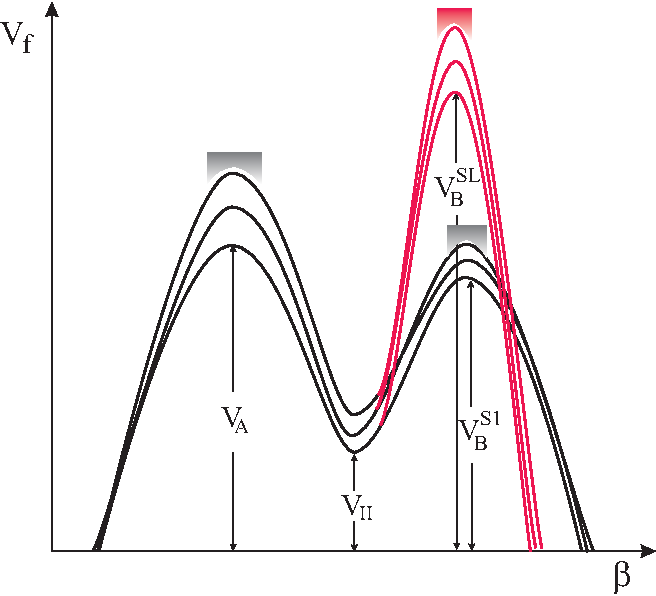
\includegraphics[width=0.5\paperwidth]{figs/emp-fis-mod}
\caption{Double-humped fission barriers used in multi-modal calculations.}
\label{fis-multimod}
\end{center}
\end{figure}
%
The parameters of the fission barriers can be retrieved from 3 files selected by the
directive input FISBAR. 
\begin{itemize}
\item{ } FISBAR=1 (default value) selects the file \textit{/RIPL/fission/empirical-barriers.dat} which contains the
fission barrier parameters for the most important preactinide and actinide nuclei.
For pre-actinides the file provides the heights for the single-humped barriers while EMPIRE adds the default
value for the width $\hbar\omega_{w2}=0.3$ MeV. For actinides are given both the heights and the widths
for the humps of double-humped barriers  The code provides for the parameters of the
isomeric well the default values $V_{w2}=$2 MeV and $\hbar\omega_{w2}=1$ MeV.
\item FISBAR=0 selects the file \textit{/data/fisbar.dat} where the user can store heights (depths) and widths for humps
and wells of single-, double- or triple-humped fission barriers.
\item FISBAR=2 selects the file \textit{/data/HFB-parab-fisbar.dat} which contains heights (depths) 
and widths for humps
and wells of single-, double- or triple-humped barriers resulted from the parabolic parametrization of
HFB numerical barriers (see next paragraph) for 59 actinides.
\end{itemize}


\paragraph{(ii) Numerical barriers}
The fission paths have been estimated within the HFB model with BSk14 Skyrme force \cite{gsp07}
for all nuclei with $90 \le Z \le 102$ lying between the valley of $\beta$-stability and the neutron 
drip lines, i.e about 1000 nuclei.  Generally, for most of the neutron-rich nuclei, three 
barriers are found.

The fission barriers, obtained by projecting the 3-D energy surfaces along the quadrupole
deformation parameter  are provided in tabular form in \textit{/RIPL/fission/HFB2007} directory. 
Generally, for most of the neutron-rich nuclei, three barriers are found.
In Figure~\ref{fis-tot-bar} are presented the HFB fission barriers of several actinides.
For an accurate description of the fission cross section the barrier can be renormalized.
The global scaling of the width of the entire barrier is reached by multiplying the quadrupole deformation
with a factor $n_{\beta}$  read from the fission input  
\begin{equation}
\beta_i= n_{\beta}\beta_i\qquad i=1,N_p
\label{w-norm}
\end{equation}
where  $N_p$ is the number of points for which the numerical barrier is defined.
\\
The global scaling of the height of the entire barrier is reached by multiplying the fission potential
with a factor $n_{h}$  read from the fission input  (see the fission Input/Output description for details)
\begin{equation}
V(\beta_i)= n_{b}V(\beta_i)\qquad i=1,N_p.
\label{b-norm1}
\end{equation}
\\
An independent normalization of each hump is realized by keeping the bottom of the well(s) unchanged 
\begin{equation}
V_h(\beta_i)= V_h(\beta_i)+ n_{b,h}V_h(\beta_i-(V(\beta))_{min})
\label{b-norm2}
\end{equation}
with $i$ running in the appropriate deformation regions.
 %
\begin{figure}[htbp]
\begin{center}
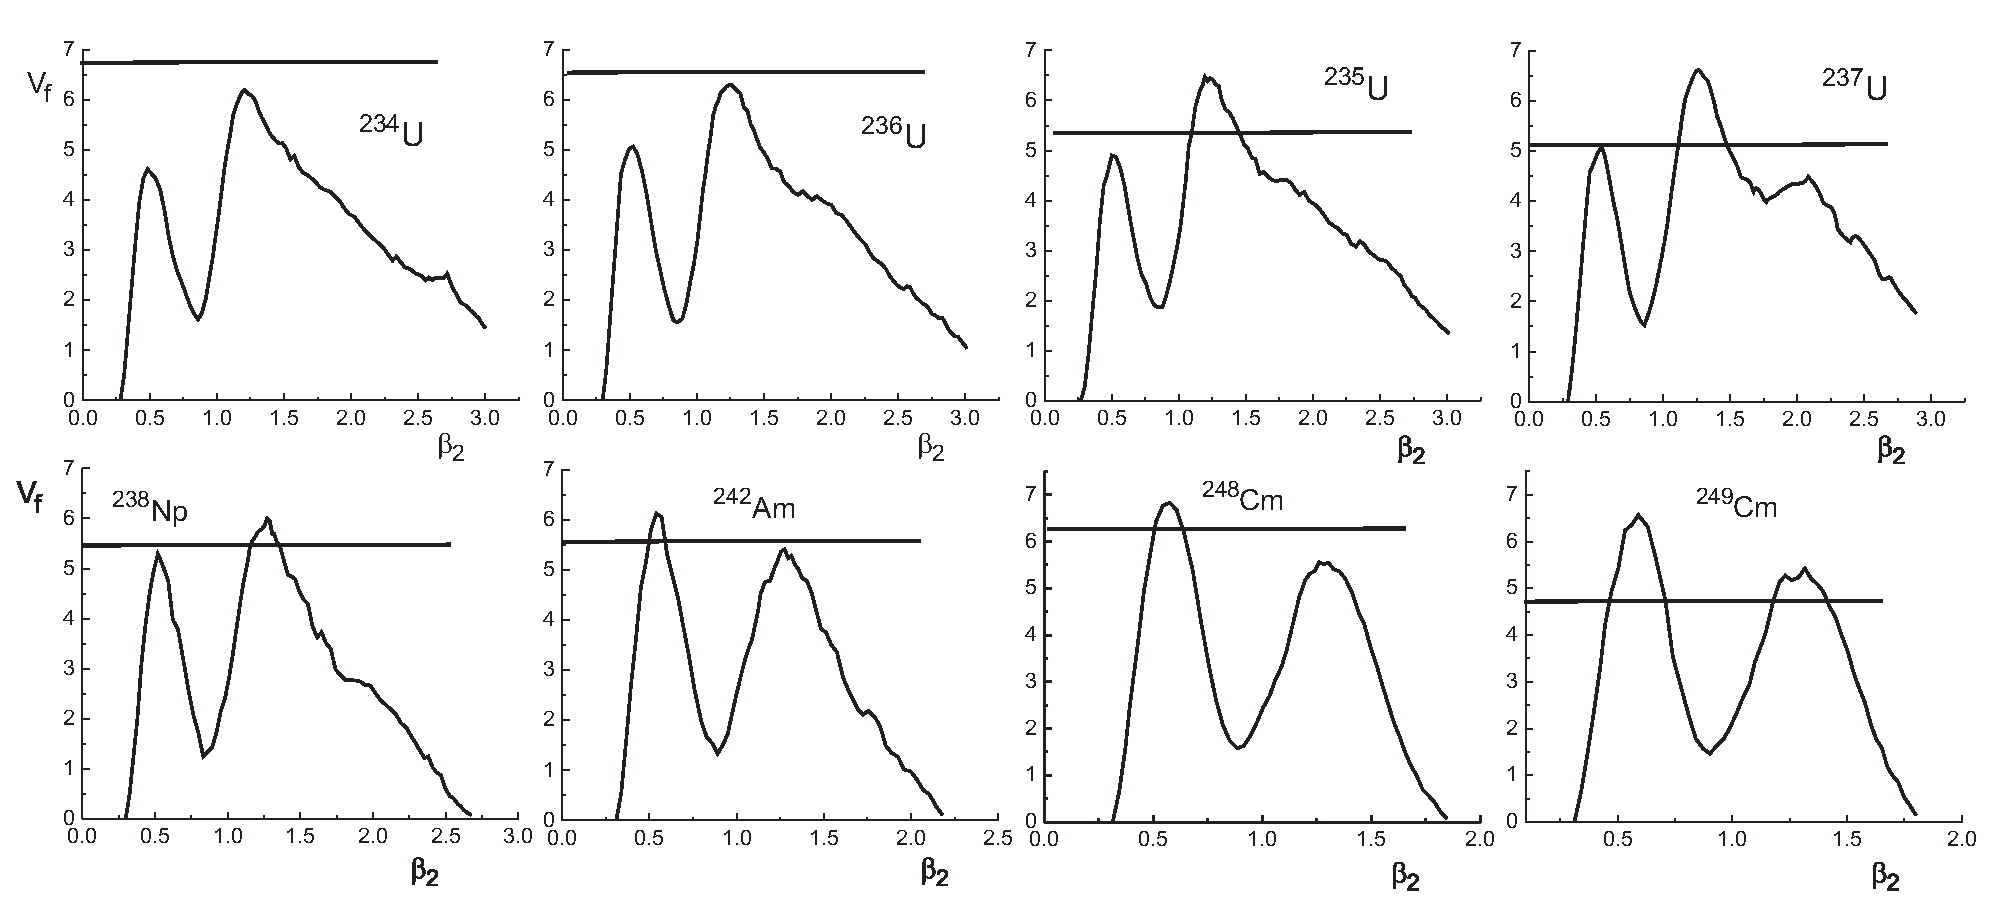
\includegraphics[width=0.7\paperwidth]{figs/emp-fis-tot-bar}
\caption{HFB fission barriers \cite{Goriely:07-mass}. The horizontal line indicates the neutron separation energy.}
\label{fis-tot-bar}
\end{center}
\end{figure}
%

Specialized subroutines for smoothing,
finding extrema points, interpolation and integration have been implemented in order
to use numerically defined barriers. This capability qualifies Empire as a valuable tool for
testing global microscopic fission parameters and for using them in applications 
requiring a blind description of fission for nuclei far from stability.

%=========================================================
\subsubsection{\bf Level densities at fission saddles}
%=========================================================
There are two types of level densities at saddles implemented in EMPIRE: one based on Enhanced Generalized 
Superfluid Model(EGSM) and the second based on Hartree-Fock-Bogoliubov + combinatorial method (HFB).
They can be selected by the directive input FISDEN.
It is recommended to use the same density model for equilibrium and saddles deformations.

\paragraph{EGSM}(FISDEN=0 default option). 
When using EGSM to describe the normal states corresponding to the 
equilibrium deformation it is natural to use the same model
to describe the level densities for the deformations specific to the
saddle points, also referred to as the level densities of the transition
states. Considering that there are no experimental data available for normalization,
the starting values of the parameters entering the transition state density 
are obtained by using physical arguments to adjust the parameters of the normal 
states at equilibrium deformation for the saddle point deformation. The final values
are deduced from the fit of the experimental data for neutron-induced fission
cross sections. 
The main differences between the density of the normal states and the density 
of the transition states are outlined below.

The calculation of the level density parameter $a_{fh}$ for the transition
states at the hump $h$ requires knowledge of its asymptotic value $%
\tilde a_{fh}$ of the damping of the shell effects $\gamma_{fh}$ and of the
shell correction $\delta W_{fi}$. All these quantities are interrelated and
depend on their corresponding values for the equilibrium deformation;
therefore, it is difficult to provide a general prescription for their
calculation. The default values of these parameters follow the recommendations
in RIPL or are deduced from previous fits of the experimental data:
\begin{itemize}
\item for the ratio of the asymptotic values of the
level density parameter at the saddle points and equilibrium deformation 
$\tilde a_f/\tilde a$ was adopted the value 1; 
\item pairing at saddles is parameterized following RIPL as $\Delta_{f}=14A^{-1/2}$,
\item the values, in MeV, for the inner and the outer barrier of the shell corrections 
recommended are calculated according to:
\begin{align}
&\delta W_{f1}=\left\{
\begin{array}{lr}
2.6           & \qquad\qquad\qquad~~~~Z\leq 97 \notag \\
2.6-0.1(Z-97) & \qquad\qquad\qquad~~~~$Z>97$
\end{array}
\right. \notag  \\ 
&\delta W_{f2}=\left\{
\begin{array}{lr}
0.6+0.1(Z-97)+0.04(N-143) & Z<97 \\
0.6+0.04(N-143) & Z\geq 97
\end{array}
\right. \label{shell_f}
\end{align}
In case of a third hump, by default $\delta W_{f3}=\delta W_{f2}$. 
\item for the the damping of the shell effects wad adopted the value $\gamma_{f}$=0.6 MeV$^{-1}$;
\item the vibrational enhacement at saddles is higher than that for equilibrium deformation roughly with
a factor of 4;
\end{itemize}
All the remaining parameters, including the
moments of inertia, have been calculated according to the formulae presented
in section~\ref{EGSM} by replacing the equilibrium deformation with the
deformations corresponding to the saddle points.

The order of symmetry of the nuclear shape at saddles has an
important impact on the transition state spectrum. This is taken into account
by multiplying the level density  by an enhancement factor $f_{sym}$
associated with the nuclear shape symmetry at each saddle and determined in Ref.~\cite{74BBM}:
\begin{equation}
f_{sym}=\left\{
\begin{array}{ll}
1 & {\rm axial,~ mirror~ symmetry}\\
\sqrt{\frac{\pi}{2}\Im_{\parallel}\cdot T} & {\rm axial~ asymmetry,~ mirror~ symmetry}\\
2 & {\rm axial~ symmetry,~ mirror ~asymmetry}\\
\end{array}
\right.
\label{f_sym}
\end{equation}
By default, the nuclear shape at the inner saddle is considered axial and mirror symmetric if the number
of neutrons is less than 144 and axial asymmetric and mirror symmetric for the rest of nuclei while
for the outer saddle(s) the shape is considered to be axial symmetric and mirror asymetric.

To overcome the shortcomings in modeling the densities of the transition
states and to provide flexibility for nuclear data evaluation there are two
posibilities to adjust the level density at each saddle:  a shift in the
efective excitation energy $U_h=E_x-E_{ch}+\Delta_f$
\begin{equation}
U_h^*=U_h+\delta_h
\end{equation}
and a global scaling factor $N_h$.
In the end, the level density at the saddle point $h$ reads:
\begin{equation}
\rho_{fh}^{EGSM}(U_h,J\pi)=\rho^{EGSM}(U_h^*,J\pi)f_{sym}N_h
\end{equation}
with the parameters entering $\rho^{EGSM}$ specific to the saddle point deformation.

It should be noted that the uncertainty of above estimates is significant~\cite{Bjornholm:80},
therefore they can be modified to reproduce the experimental data in different
energy ranges. 

\paragraph{HFB} (FISDEN=3)
\label{mic_fis}
The HFB combinatorial method developed to estimate the level densities at
ground-state deformation~\cite{09G} (see section~\ref{HFB}) has been used to
calculate coherently the level densities at the saddle points, making use of the
corresponding HFB predictions for the single-particle level scheme and
pairing strength at the corresponding deformation. 
%As suggested by mean field calculations \cite{06D}, we consider here that
%the inner barrier is triaxial and the outer barrier is left-right
%asymmetric. The corresponding enhancement factors $f_{sym}$ given by Eq.~(%
%\ref{eq_fsym3}) are taken into account.

The HFB combinatorial model level density 
\cite{09G} at each of the 2 (or 3) highest saddle point barriers and of the 1 (or
2) shape isomers are given in a table format (in an energy, spin and parity
grid identical to that for the ground-state level densities given in section~\ref{HFB})
in the directory \textit{/RIPL/fission/leveldensities/}. Each isotopic chain is
included in a \textit{zXXX.dat} file (where XXX corresponds to the atomic
number $Z$) in the subdirectories \textit{Max1/,Max2/, Max3/, Min1/, Min2/} 
corresponding to the first, second and third saddle points (sorted by
increasing quadrupole deformations) and first and second minima, respectively
(if there are only 2 barriers, the data for the third saddle and second
minimum are missing in the respective files). 
The second and third saddles as well as the second minimum are found to
be left-right asymmetric within the HFB framework. For these reasons, 
tabulated level densities have already been multiplied by a factor of 2 
(see Eq.~\ref{f_sym}). In contrast, the inner barrier and first isomer may or may not
be triaxial (note that in the HFB approach, it has been estimated using the
approximation of axial symmetry), and therefore the corresponding level density in
the tables has not been enhanced by the $f_{sym}$ (Eq.~(\ref{f_sym}))
factor. The appropriate enhancement is applied by EMPIRE. 


For many nuclear physics applications a renormalization procedure of the level densities
based on experimental data is required, in particular for nuclear data evaluation
or for an accurate estimate of reaction cross sections. Though the HFB 
combinatorial level densities at the saddle deformations are provided in a
table format, it is possible to renormalize them using a relation similar to
Eq.~(\ref{HFB-norm}) applied for the ground-state level densities
\begin{equation}
\rho^{HFB_{norm}}_{fh}(U_h,J\pi)=\exp\left(\alpha_h\sqrt{U_h-\delta_h}\right)
\rho^{HFB}_{fh}(U_h-\delta_h,J\pi)N_h.
\label{HFB-fis}
\end{equation}
The energy shift $\delta$ and the scaling factor $\alpha$ are free 
parameters  which can be adjusted at each saddle  deformation to optimize the
fit to the fission cross section. These parameters can be expected to reach
values similar to those derived for the ground-state level densities \cite{09G}, i.e.,
typically $\pm 1$~MeV for $\delta$ and $\pm 0.5~\text{MeV}^{-1/2}$ for $\alpha$.
In addition a global scaling factor $N_h$ can be applied.
These values reflect the remaining uncertainties in the level density predictions on
the basis of the mean-field combinatorial approach.

%=============================================
\subsubsection{Transmission mechanisms}
%=============================================
The single-hump transmission coefficient, $T_{h}$ is expressed in first-order 
WKB approximation in term of the momentum integral for the hump~\cite{Froman:65, FD70}:
\begin{equation}
T_{h}=\frac{1}{1+\exp(2K_{h})}
\label{single_hump}%
\end{equation}
%
with
\begin{equation}
K_{h}=\pm\left\vert \int_{a_{h}}^{b_{h}}[2\mu(E_x-V_{h}(\beta))/\hbar^{2}%
]^{1/2}d\beta\right\vert 
\end{equation}
where the $+$ sign is taken when the excitation energy is lower than the hump
under consideration and the $-$ when it is higher. In the latter case, the
intercepts are complex conjugate ( $b_{h}=a_{h}^{\ast}$) and the WKB
approximation is valid when their imaginary parts are small, \textit{i.e.},
for energies slightly higher than the hump. 
\\
As it is known, in the case of a single parabolic barrier, formula (\ref{single_hump}) yields the well-known
Hill-Wheeler transmission coefficient~\cite{Bjornholm:80}
\begin{equation}
T_{HW}=\frac{1}{1+\exp\left[  (2\pi/{\hbar\omega_h}){(V_h-E_x)}\right]
}\,,\label{HW}%
\end{equation}
which is an exact result.

For a double-humped barrier the transmission coefficient calculated in WKB approximation reads

\begin{equation}
T_{d_{(0)}}=\frac{T_1T_2}{1+2A^{1/2}\cos (2\nu_{2})+A}
\label{tdir_20}%
\end{equation}%
%
where $A=(1-T_1)(1-T_2)$ and $\nu_2$ represents the momentum integral for the well. 
In the intermediate wells, where the intercepts, $a_{j}$ and $b_{j}$, are real,
the momentum integrals depending on the real parts of the potential are
approximated as:
\begin{equation}
\nu_{w}=\int_{a_{w}}^{b_{w}}[2\mu(E_x-V_{w}(\beta))/\hbar^{2}]^{1/2}d\beta.
\end{equation}
For barriers with more than two humps, the transmission
coefficients can be calculated iteratively, using as reference the above equations.

In case of fission, the transmission through a multi-humped barrier depends on the degree of 
damping of the vibrational states in the potential minima. The extreme assumptions possible 
for a real fission potential are: 
\begin{itemize}
\item zero damping 
valid at very low excitation energies with respect to the barrier minima where $T_f=T_{d_0}$ and 
\item complete damping valid for excitation
energies close or above the barrier maxima where the humps can be considered decoupled and the
fission coefficient becomes:
\begin{equation}
\frac{1}{T_f}=\sum_h^{N_h}\frac{1}{T_h}
\label{tf-classic}
\end{equation}
\end{itemize}
Using the directive input FISOPT, one can choose between the simplified calculation corresponding
to the complete damping (FISOPT=0) and the full optical model formalism which describes partial
damping (FISOPT=1,2,3).
It should be noted that FISOPT=0 option, used in almost all reaction codes, leads to an overestimation of the 
fission cross section if is used for subbarrier excitation energies. 

In the optical model for fission by using a complex fission potential to describe the
partial damping of the vibrational states in the wells a smooth transition between the 
extreme situations described above becomes possible.
Within this model fission occurs either by direct transmission through the barrier, or by reemission into
the fission channel after absorption into the isomeric well(s) (see Figure \ref{emp-fis-mech}). 
The fission transmission coefficients associated with these two
mechanisms  are the direct transmission coefficient
($T_{d}$) and the indirect ($T_{i}$) one, respectively, the sum of their contributions representing the total
fission coefficient ($T_{f}$).

In \cite{Sin:08} is presented a recursive method to calculate the transmission coefficients through a barrier 
with $N_h$ humps and $N_w$ wells. Using the notation appropriate for recursive derivation the general
expression for the fission coefficient is 
\begin{equation}
T_f=T_d(1,N_h)+R\sum_{w=2}^{N_w} T_i(w).
\label{tf-gen}
\end{equation}
where $T_d(1,N_h)$ represents the direct transmission coefficient through all humps (starting with hump 1 and 
ending with hump $N_h$), $T_i(w)$ stands
for the indirect transmission coefficient associeted to the well $w$ and $R$ is a normalization factor
described later. 
\\
Because the general formulae are difficult to be followed and considering that for practical 
applications only the double- and triple-humped barriers are of interest, here are presented
the fission coefficients for these particular cases.
\\
\\
%=========================================
{\bf Double-humped barrier.} 
%=========================================
The incoming flux can be transmitted directly through the barrier
or can be absorbed in the isomeric well. The fraction absorbed in
the isomeric well can: (i) be re-emitted in the fission channel (indirect
prompt fission), (ii) return back to a class I state or (iii) undergo
$\gamma$-transition to the isomeric state. The isomeric state, in
turn, can decay by delayed (isomeric) fission\index{isomeric fission}
or by shape transition to class I states. In the present version of EMPIRE the 
$\gamma$-transition to the isomeric state and hence the delayed fission are not
considered. They are going to be implemented soon because they might make a difference
in those cases where the compound nucleus is populated in states with small excitation energies
with respect to the bottom of the isomeric well, as could happen in photofission.

In the case of a double-humped barrier, the general expression of the fission coefficient given in Eq.\ref{tf-gen} 
becomes
\begin{equation}
T_f=T_d(1,2)+RT_i(2)= T_d(1,2)+T_a\frac{T_d(2,2)}{\sum T(2)},\qquad R=1
\label{tf2}
\end{equation}
%
The expression of the direct transmission coefficient through a
double-humped barrier in the presence of absorption is a generalization of Eq.\ref{tdir_20}.
It is obtained by adding to the real momentum integrals $\nu_w$ the imaginary contributions
$\delta_w$ corresponding to the imaginary potential  \cite{Bhandari:79}
%
\begin{equation}
\delta_w=-\left(  \frac{\mu}{2\hbar^{2}}\right)  ^{1/2}\int_{a_{w}}^{b_{w}%
}\frac{W_w(\beta)}{[E-V_{w}(\beta)]^{1/2}}d\beta\,\quad
w=2,
\end{equation}

\begin{equation}
T_{d}(1,2)= \frac{T_{d}(1,1)T_{d}(2,2)}
                    {e^{2\delta_2} + 2A^{1/2}\cos(2\nu_2)+Ae^{-2\delta_2}}
\label{tdir2}                    
\end{equation}
where $A=[1-T_d(1,1)][1-T_d(2,2)]$ 
and $T_d(h,h)$ represents the transmission coefficient
through the hump $h$ given by the Hill-Wheeler formula (Eq.\ref{HW}).
\\
The absorption coefficient for a double humped barrier is 
\begin{equation}
T_{a}(1,2)= T_{d}(1,2)\left[e^{2\delta(2)}-\frac{[1-T_{d}(2,2)]
                                   e^{-2\delta(2)}}{T_{d}(2,2)}\right].
\end{equation}
where the notation $T_a(1,2)$ stands for the absorption coefficient describing the 
shape transition from minimum 1 to minimum 2.
The denominator of the second term in Eq.\ref{tf2} stands for the sum of the transmission coefficients
for the competing channels specific to the second well
\begin{equation}
\sum T(2)=T_d(1,1)+T_d(2,2).
\end{equation}
AS mentioned before, the gamma-decay in the isomeric well was neglected. 
%
\begin{figure}[htbp]
\begin{center}
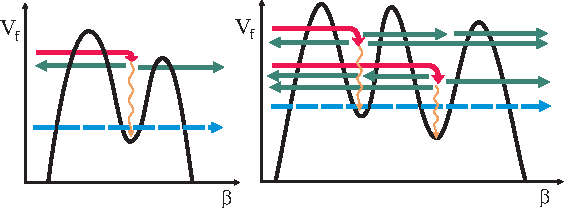
\includegraphics[width=0.7\paperwidth]{figs/emp-fis-mech}
\caption{Transmission mechanisms through  double- and triple-humped fission barriers.}
\label{emp-fis-mech}
\end{center}
\end{figure}
%
%\begin{figure}[htbp]
%\scalebox{0.7}{\includegraphics{emp-3mec1.eps}}
%\caption{\label{cap:Transmission-mechanisms-through-triple}Transmission mechanisms
%through a triple-humped fission barrier}
%\end{figure}
\\
%=========================================
{\bf Triple-humped barrier.} 
%=========================================
The general expression of the fission coefficient given in Eq.\ref{tf-gen} 
becomes in the case of a triple-humped barrier
\begin{equation}
T_f=T_d(1,3)+R[T_i(2)+T_i(3)],
\end{equation}
The direct transmission coefficient through all the humps is calculated using Eq.\ref{tdir2}
in which the transmission through the outer hump $T_d(2,2)$ is replaced with the direct transmission
through the outer humps $T_d(2,3)$


\begin{equation}
T_{d}(1,3)= \frac{T_{d}(1,1)T_{d}(2,3)}
                    {e^{2\delta_2} + 2A^{1/2}\cos(2\nu_2)+Ae^{-2\delta_2}}
\label{tdir13}                    
\end{equation}
where $A=[1-T_d(1,1)][1-T_d(2,3)]$ and
\begin{equation}
T_{d}(2,3)= \frac{T_{d}(2,2)T_{d}(3,3)}
                    {e^{2\delta_3} + 2A^{1/2}\cos(2\nu_3)+Ae^{-2\delta_3}}
\label{tdir23}                    
\end{equation}
where $A=[1-T_d(2,2)][1-T_d(3,3)]$. 






\begin{equation}
T_i(2)=T_a(1,2)
           \left[\frac{T_{d}(2,3)}{\sum T(2)} +
                 \frac{T_{a}(2,3)}{\sum T(2)}\cdot
                 \frac{T_{d}(3,3)}{\sum T(3)}\right]R
\end{equation}
\begin{equation}
T_i(3)=T_a(1,3)
           \left[\frac{T_{d}(3,3)}{\sum T(3)} +
                 \frac{T_{a}(3,2)}{\sum T(3)}\cdot
                 \frac{T_{d}(2,3)}{\sum T(2)}\right]R.
\end{equation}


 \
The forward absorption coefficients are calculated in terms of direct transmission 
coefficients across the humps on the right sides of the corresponding wells:

\begin{equation}
T_{a}(1,2)= T_{d}(1,3)\left[e^{2\delta(2)}-\frac{[1-T_{d}(2,3)]
                                   e^{-2\delta(2)}}{T_{d}(2,3)}\right].
\end{equation}

\begin{equation}
T_{a}(1,3)= T_{d}(1,3)\left[e^{2\delta(3)}-\frac{[1-T_{d}(3,3)]
                                   e^{-2\delta(3)}}{T_{d}(3,3)}\right].
\end{equation}

\begin{equation}
T_{a}(2,3)= T_{d}(2,3)\left[e^{2\delta(3)}-\frac{[1-T_{d}(3,3)]
                                   e^{-2\delta(3)}}{T_{d}(3,3)}\right].
\end{equation}
\\
The backward absorption coefficient from the well 3 into the well 2 
is calculated in terms of the direct transmission coefficients across the humps 
on the left sides of the two wells:

\begin{equation}
T_{a}(3,2)= T_{d}(2,1)\left[e^{2\delta(2)}-\frac{[1-T_{d}(1,1)]
                                   e^{-2\delta(2)}}{T_{d}(1,1)}\right].
\end{equation}


The sum of the transmission coefficients for the competing channels specific
to the wells 2 and 3 are

\begin{equation}
\sum T(2)=T_d(1,1)+T_d(2,3)+T_a(2,3)   %+T_{\gamma}(2)
\end{equation}

\begin{equation}
\sum T(3)=T_d(2,1)+T_d(3,3)+T_a(3,2)   %+T_{\gamma}(3)
\end{equation}


\begin{equation}
R=\left[1-\frac{T_a(2,3)}{\sum T(2)}\frac{T_a(3,2)}{\sum T(3)}\right]^{-1}.
\label{r}
\end{equation}
%=============================================
\subsubsection{Effective fission coefficients}
%=============================================
The fission coefficients presented up to now correspond to transmission through a single barrier $(K,J\pi)$.
In Eq.~\ref{pfis} enters the fission coefficient corresponding to the transmission through all barriers characterized
by the quantum numbers $J\pi$. The calculation of this effective fission coefficient is described below.  

The structure of the saddle transition states is complex and still difficult to be predicted accurately. It depends
on the odd-even-A type and on the asymmetries of the nuclear shape at saddle deformation.   
In the present formalism we atempt to keep the spirit of the optical model for fission and also the fission input manageable 
by the users but to consider in the same time the partial lift of degenaracy associated to the nuclear shape asymmetry.
The idea was to apply to the discrete transition states the same enhancement factors as for the density functions which 
describe the transition states in continuum. Obviously, due to the spin-parity selection rules, this method is not
equivalent to taking into account properly  the double degeneracy of the $K^{\pi}$ bands at the outer saddle(s) for instance,
but our tests indicated that the impact on the fission cross section is similar.
Because the transmission coefficients calculation in the optical model for fission requiers a full fission path along the
quadrupole deformation, the enhancements were applied on the transmission coefficients and not on the discrete levels.


The total transmission coefficient through one hump is sum of two contributions
corresponding to the discrete and continuous part of the transition
state spectrum
\begin{equation}
T_{h}(EJ\pi)=\sum_{K\leq J}d_{sym}(h)T_{h}(EKJ\pi)+\int_{E_{ch}}^{\infty}
\frac{\rho_h(\varepsilon J\pi)d\varepsilon}
     {{1+\exp\left[-\frac{2\pi}{\hbar\omega_{h}}(E-V_{h}-\varepsilon)\right]}}\quad h=1,N_h
\label{tjt}
\end{equation}
where
\begin{equation}
T_h(EKJ\pi )=T_d(h,h)
\end{equation}
and the enhancement $d_{sym}(h)$ reads
\begin{equation}
d_{sym}=\left\{
\begin{array}{ll}
1 & {\rm axial,~ mirror~ symmetry}\\
2J+1 & {\rm axial~ asymmetry,~ mirror~ symmetry}\\
2 & {\rm axial~ symmetry,~ mirror ~asymmetry}\\
\end{array}
\right..
\label{d_sym}
\end{equation}

 Increasing the excitation energy, the strength of the imaginary potential
increases and the entire flux transmitted through the inner hump is
absorbed in the second (isomeric) well ($T_{abs}\rightarrow T_{A}$),
and the direct transmission through the entire barrier disappears
($T_{dir}\rightarrow0$). Therefore, the direct fission occurs only
for sub-barrier excitation energies and occurs only through discrete
channels
\begin{equation}
T_{dir}^{(h,h')}(EJ\pi )=\sum _{K\leq J}{\rm min}\left(d_{sym}(h),d_{sym}(h')\right) T_{dir}^{(h,h')}(EKJ\pi )
\end{equation}
where
\begin{equation}
T_{dir}^{(h,h')}(EKJ\pi )=T_d(h,h')\qquad h\not=h';\quad h,h'=1,N_h
\end{equation}


For the indirect fission coefficient, the way the sum rule applies depends on the assumptions
concerning the preservation of the quantum number $K$ in the isomeric well(s).
In the description of fission cross sections, one can consider two extreme
limits: the first limit assumes that fission mainly proceeds through discrete
transition states characterized by well-defined values of $K$ and is known as
``no K-mixing'' approximation; the second limit considers that the excitation of
internal degrees of freedom in the second well makes it possible for the
nucleus to change its $K$ value during the time the energy is bound in
internal motions and this effect is referred to as ``full K-mixing''. The effect
of these approximations on the fission probability is very small, but they can
affect significantly the angular correlations of the fission fragments
~\cite{Back:74}. The appropriate choice for the purpose of nuclear data
evaluation is the ``full K-mixing'' approximation, not only for physical
reasons, but also because it can be applied for any excitation energy. 
Formally, ``full K-mixing'' is described by adding the absorption from different
transition states irrespective of the associated $K$ value into a quantity
preserving the spin and parity. 
The continuum fission channels
contribute at higher energies, where the class II states are completely
damped and the entire flux transmitted through the inner barrier is
absorbed in the isomeric\index{isomeric fission} well.
The main consequence is that the absorption
coefficient for a certain $J\Pi$ is:
\begin{equation}
T_{abs}^{(w,w')}(EJ\pi)=\sum_{K\leq J}d_{sym}(h)T_{abs}(EKJ\pi)
+\int_{E_{ch}}^{\infty}\frac{\rho_{h}(\varepsilon J\pi)d\varepsilon}
                            {{1+\exp\left[-\frac{2\pi}{\hbar\omega_{h}}(E-V_{h}-\varepsilon)\right]}}
                            \quad h=w
\label{tabst}
\end{equation}
with
\begin{equation}
T_{abs}^{(w,w')}(EKJ\pi )=T_a(w,w') \qquad w\not= w' %=1,W;\quad w,w'=2,H
\end{equation}

The optical model for fission provides a realistic description of the fission
cross section, including the resonance structure at subbarrier excitation energies due to the
coupling among discrete vibrational states in different wells. Therefore, the model is recommended to
be used when high accuracy in description of the experimental data is required. 
As mentioned before, in such cases,
the parameters of the fission barriers associated to the transition states are considered free
parameters and their values are extracted from systematics or from the fit of the experimental
data. Even if the predictive power of the model is not very good, the descriptive power could be
impressive.
%&&&&&&&&&&&&&&&&&&&&&&&&&&&&&&&&&&&&&&&&&&&&&&&&&&&&&
\paragraph*{Surrogate optical model for fission.}
%&&&&&&&&&&&&&&&&&&&&&&&&&&&&&&&&&&&&&&&&&&&&&&&&&&&&&
In most of the cases, there are no available information about the barriers' parameters
associated to the discrete transition states, therefore the transition state spectra are
considered exclusively continuous and described by density functions. Analyzing the expressions
of the fission coefficients in the previous paragraph, it can be easily noticed that the
coupling among the vibrational states in the wells, determined by the degree of their damping,
is contained only in the discrete terms. By cutting them, the general expression of the fission
coefficient reduces to Eq.\ref{tf-classic} which corresponds to full damping, or in other words,
 to decoupled
transmissions through independent humps (Figure`\ref{fis-ld0.eps}.a). 
Using this expression would overestimate fission cross
section of fertile nuclei at low energies. To overcome this disadvantage, in EMPIRE was
implemented an alternative way to consider partial damping, which does not involve imaginary
potential or discrete transition states. 
In this surrogate of the optical model for fission, the degree of
damping is taken into account by defining the total fission coefficient as a weighted sum 
of the direct coefficient corresponding to zero-damping and the indirect coefficient
corresponding to full damping     
%
\begin{equation}
T_{f}(E_x J \pi)=(1-p(E_x))T_{dir_{(0)}}^{cont}(E_x J \pi)+p(E_x)T_{ind_{(f)}}^{cont}(E_x J \pi).
\label{tfsurr}
\end{equation}
%
The term $T_{dir_{(0)}}^{cont}$ describes the direct transmission without absorption through
barriers associated to transition states in continuum. In order to calculate it, a level
density describing the entire fission barrier would be needed (Figure~\ref{fis-ld0.eps}.b). 
Making the assumption that the direct transmission
is controlled by the minimum level density at saddles the direct fission coefficient is
calculated as  
%
\begin{equation}
T_{dir}^{cont}(E_xJ\pi)=\int_0^{\infty}T_{dir_{(0)}}(\varepsilon J \pi)\rho_{min} (\varepsilon J \pi)
d \varepsilon
\end{equation}
where $T_{dir_{(0)}}$ is given by Eq.\ref{tdir_20}. 
The indirect coefficient $T_{ind_{(f)}}^{cont}$ is calculated with Eq.\ref{tf-classic}, where $T_A$ and $T_B$ are given by the
second term in Eq.\ref{tjt}.
The weight $p(E_x)$ ranges from 0 for excitation energies close to the
bottom of the well(s) to 1 for excitation energies close to the height of the lowest hump
\cite{Sin:07}. 
%
\begin{figure}[htbp]
\begin{center}
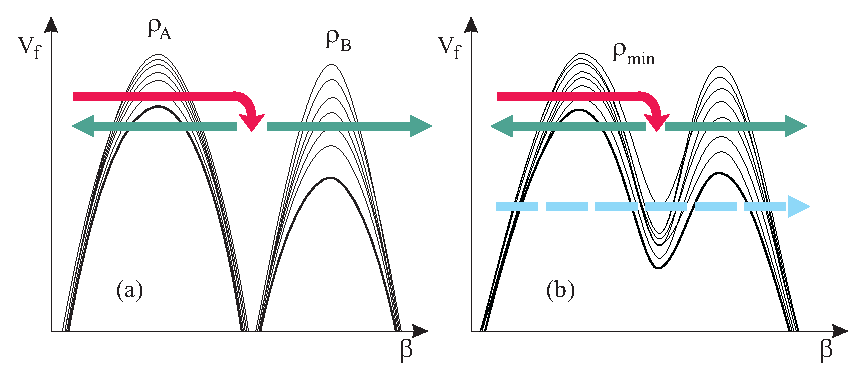
\includegraphics[width=0.7\paperwidth]{figs/emp-fis-ld0}
\caption{Illustration of the transmission mechanisms through fission barriers:
(a) decoupled transmissions through independent humps,
(b) direct transmission at low energies (dashed arrow) and decoupled transmissions at 
energies comparable or higher than the barrier height (full arrows).}
\label{fis-ld0.eps}
\end{center}
\end{figure}
%
Compared to the optical model for fission, this alternative approach has the advantage that
describes the direct and indirect fission mechanisms without involving many parameters.
It can be used also when discrete transition states are considered, but the resonant
structure is not equally well reproduced. In the optical model for fission, with increasing
energy  the imaginary potential strength increases and the resonances get damped 
(become wider and flatter until they disappear). In the surrogate approach the resonances,
coming from the direct term, remain undamped, only their contribution diminishes together
with the increase of the weight $p$.  

It is recommended to use this model when only information about the fundamental barrier and
the level densities at saddles are available. The model was used to test microscopic
barriers defined numerically \cite{Sin:07}, a relevant example being presented in
Figure~\ref{am41-surr}.
%
\begin{figure}[htbp]
\begin{center}
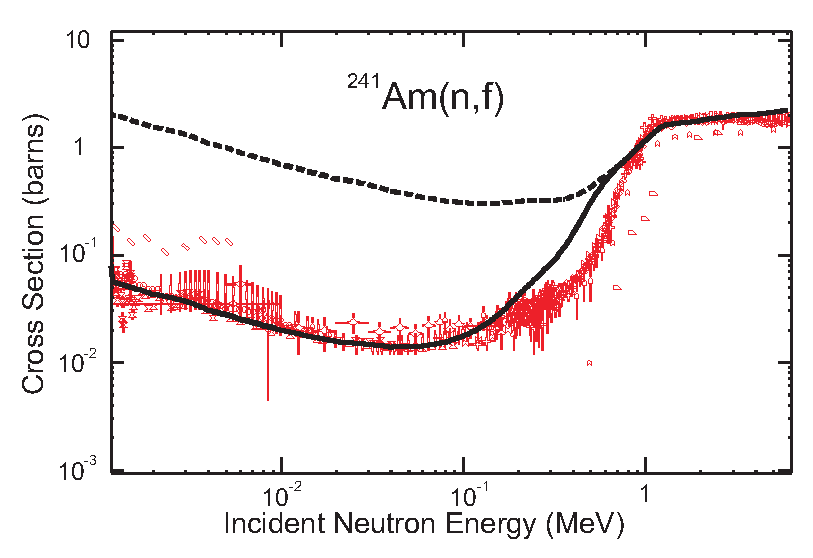
\includegraphics[width=0.7\paperwidth]{figs/emp-am41-surr}
\caption{Neutron induced fission cross section of $^{241}$Am calculated with microscopic
fission barrier \cite{Goriely:07-mass} and level densities at saddles \cite{Goriely:07-ld}. 
The full curve was obtained using Eq.\ref{tfsurr} and dashed curve was obtained using 
Eq.\ref{tf-classic}.}
\label{am41-surr}
\end{center}
\end{figure}
%


%=========================================================================
\subsubsection{Multi-modal fission}

In multi-modal fission different discrete and continuous spectra
for the transition states at the outer saddle are considered for each
mode. In Empire code are considered 3 modes: the super-long symmetric (SL) to
which is associated a high and narrow barrier where the nuclear shape is supposed to be
mass symmetric and 2 standard mass asymmetric (S1) and (S2).  

In the multi-modal fission the total fission probabiliy is the sum of each mode
contribution
\begin{equation}
P_{f}=\sum_{m}P_{f,m}
\end{equation}
with
\begin{equation}
P_{f,m}=M_{m}\cdot\frac{T_{f}}{T_{f}+\sum_{d}T_{d}}
\label{wm}
\end{equation}
\noindent where $M_{m}$ is the mode weight ($M_{m}=T_{h2,m}/\sum_{m}T_{h2,m}$)
and $T_{f}$ is the total fission coefficient
\begin{equation}
T_{f}=\frac{T_{h1}\sum_{m}T_{h2,m}}{T_{h1}+\sum_{m}T_{h2,m}}.
\end{equation}

The multi-modal fission is selected by the key input FISMOD$>0$: FISMOD=1 stands
for (SL) + (S1) (illustrated in Figure~\ref{fis-multimod}) and FISMOD=2 for
(SL) + (S1)+ (S2).
It is implemented only for two humped barrier, for EGSM saddle-densities and in the limit of
full damping (FISOPT=0).
%===============================================================

%=======================================================================
\subsection{Sierk model for fission (FISSHI=1)}
%=======================================================================

\subsubsection{Fission barriers}

The liquid-drop spin dependent fission barriers for 19$<$Z$<$102
are calculated using the BARFIT subroutine~\cite{sierk}, which also
provides ground state energies and the compound nucleus stability
limit with respect to fission (i.e., spin value at which liquid-drop
fission barrier disappears). BARFIT consists of a fit to the barriers
calculated by Sierk within the rotating droplet model, using Yukawa-plus-exponential
double folded nuclear energy, exact Coulomb diffuseness corrections,
and diffuse-matter moments of inertia. The calculated barriers for
\emph{l} = 0 are accurate to a little less than 0.1 MeV. The output
from the BARFIT subroutine is a little less accurate. Errors may be
as large as 0.5 MeV but the characteristic uncertainty is in the range
of 0.1-0.2 MeV. The values of ground state energy are generally approximated
to within about 0.1-0.2 MeV. The approximate value of the stability
limit is nearly always within 0.5$\hbar$ of the calculated one. 

For nuclei with Z$\geq$102 the recent parametrization of the Thomas-Fermi
fission barriers at zero spin is used \cite{MSbarr} . \begin{equation}
B_{f}(J=0)=S(N,Z)F(X),\label{MSbar0}\end{equation}
where \emph{S} is proportional to the nominal surface energy of the
nucleus, and is given by\begin{equation}
S=A^{2/3}(1-kI^{2}),\end{equation}
with $I=(N-Z)/A$ and $k=1.9+(Z-80)/75$. The fissility is proportional
to the ratio of the nominal Coulomb and surface energies of a sphere:\begin{equation}
X=Z^{2}/A(1-kI^{2}).\end{equation}
The function \emph{F} is\begin{equation}
\begin{array}{ll}
F(X)=0.000199749(X-X_{0})^{3} & \,\, for\,\, X_{1}\leq X\leq X_{0}\\
F(X)=0.595553-0.124136(X-X_{1}) & \,\, for\,\,30\leq X\leq X_{1}\end{array}\label{MSbar1}\end{equation}
 with $X_{0}=48.5428$ and $X_{1}=34.15$. These formulae predict
vanishing barriers for nuclei with Z$\geq110$. Spin dependence is
not provided by Eqs. \ref{MSbar0}-\ref{MSbar1}. The EMPIRE code
assumes that angular momentum dependence calculated with BARFIT for
Z=102 and A=256 is also valid for the heavier nuclei. 

The full fission barrier is a sum of the liquid-drop part and the
shell correction $\delta_{W}$ taken with the opposite sign. The latter
is assumed to gradually disappear with spin \emph{J} and temperature
\emph{T} so that the fission barrier becomes

\begin{equation}
B_{f}\left(T,J\right)=B_{ld}\left(J\right)-f\left(T\right)g\left(J\right)\delta_{W}.\end{equation}
The temperature fade-out function was found \cite{fade} to be\begin{equation}
\begin{array}{ll}
f\left(T\right)=1 & \,\, for\,\, T<1.65MeV\\
f\left(T\right)=e^{1.066(1.65-T)} & \,\, for\,\, T\geq1.65MeV.\end{array}\label{BfTfade}\end{equation}
For the angular momentum fade-out the following formula is used \cite{fade}
\begin{equation}
g\left(J\right)=\frac{1}{1+\exp\left[\left(J-J_{1/2}\right)/\Delta J\right]}+d\cdot\exp\left[\left(J-J_{G}\right)^{2}/\Delta J_{G}^{2}\right]\,,\label{BfJfade}\end{equation}
where the first term accounts for the overall decrease of the shell
correction due to the increasing nuclear deformation, while the second
one (of Gaussian type) permits the inclusion of fluctuations characteristic
of the particular nucleus. The parameters $J_{1/2}$ and $\Delta J$
vary slowly with the mass number. Typical values for heavy nuclei
are about 20-25 for $J_{1/2}$ and 2-3 for $\Delta J$. The Gaussian
correction can be used only if the relevant parameters can be determined
from the experimental data.

The saddle-point moments of inertia are calculated using Sierk's routine
MOMFIT \cite{sierk}, which provides a fit to the advanced liquid-drop
model calculations as mentioned in subsection \ref{sec: defor}.

\subsubsection{Dissipation effects}

The fission process is delayed by the dissipation effects. They are
treated in an approximate, time-independent approach~\cite{grange,rastop,kram},
which takes into account: (i) the stationary limit of Kramers \cite{kram}
and (ii) the exponential factor \cite{rastop} applied to the Kramers'
fission width to account for the transient time after which the statistical
regime is reached. The classical Hill-Wheeler\index{Hill-Wheeler}
fission width $\Gamma_{f}^{HW}$ (Eq. \ref{fwidth}) is modified to
obtain Kramers limit

\begin{equation}
\Gamma_{f}^{K}=\Gamma_{f}^{HW}(\sqrt{1.0+(\beta_{v}/2\hbar\omega)^{2}}-\beta_{v}/2\hbar\omega)\label{diss1}\end{equation}


\noindent where $\beta_{v}$ is the reduced dissipation coefficient
and $\omega$ describes the potential curvature at the fission saddle
point. In addition, the fission width is reduced to account for the
transient time needed to form a saddle point \cite{rastop}

\begin{equation}
\Gamma_{f}=\Gamma_{f}^{K}\exp\biggl(-1.51768\tau\sum_{x}\Gamma_{x}\biggr),\label{diss2}\end{equation}


\noindent where $x$ runs over all particle channels and $\tau$ is
given by\begin{equation}
\begin{array}{cc}
\tau=\beta_{v}^{-1}ln(10\frac{B_{f}}{T}) & for\,\,\beta_{v}<3.2\cdot10^{-21}\, s^{-1}\\
\tau=0.19531\beta_{v}ln(10\frac{B_{f}}{T}) & for\,\,\beta_{v}\geq3.2\cdot10^{-21}\, s^{-1}\end{array}\label{Rstopvisc}\end{equation}
$T$ is a nuclear temperature, and $\beta_{v}=3.2\cdot10^{-21}\, s^{-1}$
is assumed to separate under-damped and over-damped motion.


\subsection{Prompt Fission Neutrons}
\label{pfns}

The prompt fission neutrons play an important role in neutronics calculations for nuclear applications.
It has been shown that estimated uncertainties in the prompt fission neutron spectrum can significantly impact the results of transport simulations
for critical assemblies as well as reactor sensitivity calculations \cite{Talou:2011b}.  The main difficulty
with the modeling of prompt fission neutron spectra (PFNS) is that their shape is not well defined experimentally.
In addition, it is also important to know the PFNS as a function of both the fissioning
nucleus and its excitation energy.  Due to this sensitivity, PFNS has to be included in the adjustment to avoid unphysical modification of other quantities, e.g., fission cross sections, that might result from compensating deficiencies in the PFNS. In the current version of the EMPIRE code we have implemented PFNS calculations using Los Alamos and Kornilov models. We have decided to include both formulations since there is a controversy regarding the lower energy part of the spectra - the Los Alamos model tends to predict lower values versus the Kornilov model. So far integral testing was mixed and there is no clear evidence which of the two models is more adequate. 




\subsubsection{Los Alamos model for prompt fission neutron spectra}

The Madland-Nix or Los Alamos model~\cite{Madland:82} constitutes the basis for the evaluation
of prompt fission neutrons spectra in most current evaluated nuclear data libraries.
 According to the Los Alamos model \cite{Madland:82}, both the Watt
and Maxwellian spectra neglect two important physical effects: 1) the distribution of fission-fragment
residual nuclear temperature that results from the initial distribution of fission-fragment excitation
energy and the subsequent cooling of the fragments as neutrons are emitted and 2) the energy dependence
of the cross section for the inverse process of compound nucleus formation. Furthermore,
the Maxwellian spectrum also neglects the center-of-mass motion of the fission fragments from which the
neutrons are emitted; therefore, the agreement between spectra and data is achieved by adjusting
parameters to values that are somewhat unphysical.   The Los Alamos model addresses
these inconsistencies by taking the distribution of fission-fragment residual nuclear temperature to be
triangular in shape, extending linearly from zero to a maximum value T$_{m}$, and calculating the
energy-dependent compound nucleus cross section for representative average fission fragments by use of
an optical model.  This permits $N(E)$ to be calculated easily for any fissioning nucleus
at any excitation energy.  Weisskopf statistical
evaporation theory \cite{Weisskopf:37} is used to explain the emission of neutrons from an excited compound
nucleus (CN) at a given temperature $T$, and a triangular distribution of initial fission 
fragments residual temperatures is assumed.

This model is the basis for  evaluation
of prompt fission neutrons spectra in most currently evaluated nuclear data libraries.
This  relatively simple and compact formalism, with only a handful of adjustable parameters, 
has been very successful in predicting the prompt fission neutrons spectra for neutron-induced as well as 
spontaneous fission reactions for a wide range of actinides and incident neutron energies. 
More refined and/or elaborate versions of the Los Alamos model have been developed in recent years for 
evaluation purposes, but they all rely on the implementation of this model in the first place. 
The Los Alamos (LA) model is described at length in Ref.~\cite{Madland:82}.
We will only summarize its main features here. 



%-- LA MODEL: c.m. neutron energy spectrum
\paragraph{Center-of-mass neutron energy spectrum.}
The neutron energy spectrum in the center-of-mass of a fission fragment is given by
\begin{eqnarray} \label{eq:cmspec}
\phi(\epsilon) = \frac{2\sigma_c(\epsilon)\epsilon}{T_m^2}\int_0^{T_m}k(T)T exp(-\epsilon/T)dT
\end{eqnarray}
with the temperature-dependent normalization constant $k(T)$
\begin{eqnarray} \label{eq:k(T)}
k(T)^{-1} = \int_0^\infty \sigma_c(\epsilon) \epsilon exp(-\epsilon/T) d\epsilon. 
\end{eqnarray}
$\sigma_c(\epsilon)$ is the energy-dependent cross section for the inverse process of CN formation. 
Equation~(\ref{eq:cmspec}) was obtained by integrating over a triangular distribution of temperatures with
a maximum temperature $T_m$.

%-- LA MODEL: lab neutron energy spectrum
\paragraph{Laboratory neutron energy spectrum.}
In the laboratory system, the neutron energy spectrum $N(E)$ for a fission fragment moving with a kinetic 
energy per nucleon $E_f$ is
\begin{eqnarray} \label{eq:cm2lab}
N(E)=\frac{1}{4\sqrt{E_f}}\int_{\left( \sqrt{E}-\sqrt{E_f} \right)^2}^{\left( \sqrt{E}+\sqrt{E_f} \right)^2}
\frac{\phi(\epsilon)}{\sqrt{\epsilon}}d\epsilon, 
\end{eqnarray}
where $E$ is the laboratory neutron energy.

Inserting (\ref{eq:cmspec}) into (\ref{eq:cm2lab}), the laboratory neutron energy spectrum $N(E)$ becomes
\begin{eqnarray} \label{eq:labspec}
N(E) = \frac{1}{2\sqrt{E_f}T_m^2} \int_{\left( \sqrt{E}-\sqrt{E_f} \right)^2}^{\left( \sqrt{E}+\sqrt{E_f}
\right)^2}\sigma_c(\epsilon)\sqrt{\epsilon}d\epsilon \\ \nonumber
\times \int_0^{T_m}k(T)Texp(-\epsilon/T)dT,
\end{eqnarray}
with $k(T)$ given by Eq.~(\ref{eq:k(T)}).

\bigskip
Considering the most probable fragmentation only, the average center-of-mass neutron energy spectrum 
$\phi(\epsilon)$ is therefore given by an average over the spectra for the light and heavy fragments as 
\begin{eqnarray}
\phi(\epsilon) = \frac{1}{2}\left( \phi_L(\epsilon) + \phi_H(\epsilon) \right),
\end{eqnarray}
and similarly for the laboratory neutron energy spectrum $N(E)$
\begin{eqnarray}
N(E) = \frac{1}{2}\left( N_L(E) + N_H(E) \right).
\end{eqnarray}
In the last two equations, it is implicitly assumed that half of the emitted neutrons come from the 
light fragment and the other half from the heavy fragment.

%-- LA MODEL: average prompt neutrons multiplicity
\paragraph{Average prompt neutrons multiplicity.}
The average prompt fission neutrons multiplicity $\overline{\nu}_p$ is simply obtained from energy 
conservation:
\begin{eqnarray}
\overline{\nu}_p=\frac{\left<E^*\right>-\left<E_\gamma^{tot}\right>}{\left<S_n\right>+\left<\epsilon\right>},
\end{eqnarray}
where $\left<E^*\right>$ is the average total excitation energy and is equal to
\begin{equation}
\left<E^*\right>=\left<E_r\right> + B_n + E_n - \left<E_f^{tot}\right>.
\end{equation}
$\left<E_r\right>$ is the average fission energy release, $B_n$ is the neutron binding energy of the target nucleus, 
$E_n$ is the neutron incident energy, $\left<E_{f}^{tot}\right>$ is the average total fission-fragment kinetic energy, 
$\left<E_\gamma^{tot}\right>$ is the average total energy carried away through gamma-ray emission, $\left<S_n\right>$ is the 
average neutron separation energy of the fission fragments, and $\left<\epsilon\right>$ is the average energy of the 
outgoing neutron in the center-of-mass reference frame.


%-- LA MODEL: Multiple-chance fission
\paragraph{Multiple-chance fission.}

At higher incident neutron energies, above the neutron binding energy, the excited compound system may 
emit one or several neutrons before undergoing fission. Although the neutrons emitted prior to fission 
are not directly related to the ones emitted from the fission fragments, in the LA model they are treated 
in a similar way. In the case of multiple-chance fission, the prompt fission neutron spectrum in the 
laboratory system can be written as
\begin{eqnarray}
N(E)=\frac{\sum_i{P_f^i\left( \sum_{j=1}^{i-1}{\phi_j(E)} +\overline{\nu}_iN_i(E) \right)}}
{\sum_i{P_f^i(i-1+\overline{\nu}_i)}}
\end{eqnarray}
where $\phi_j(E)$ is the pre-fission evaporation spectrum for the $(j+1)^{th}$-chance fission channel, 
and $P_f^i$ is the $i^{th}$-chance fission probability.

\bigskip
The average prompt neutron multiplicity can be obtained similarly
\begin{eqnarray}
\overline{\nu}=\frac{\sum_i{P_f^i(i-1+\overline{\nu}_i)}}{\sum_i{P_f^i}}
\end{eqnarray}
The $i^{th}$ prompt neutron multiplicity $\overline{\nu}_i$ is given by
\begin{eqnarray}
\overline{\nu}_i = \frac{\left< E_i^*\right>-\left< E_{\gamma_i}^{tot}\right>}{\left< S_n^i \right>+
\left< \epsilon_i \right>},
\end{eqnarray}
where the average total excitation energy for the $i^{th}$-chance fission is
\begin{eqnarray}
\left<E^*_i\right> & = & \left< E_r^i \right> + B_n(A)+E_n-\left<E_f^i\right> \nonumber \\
& & - \sum_{j=1}^{i-1}{\left( B_n(A-j+1)+\left<\epsilon_j\right> \right)}
\end{eqnarray}
Here, $\left<\epsilon_j\right>$ it the mean kinetic energy of the neutron evaporated from the $(Z,A-j+1)$ nucleus.




\subsubsection{Kornilov model for prompt fission neutron spectra}
\label{sec:korn}

The Kornilov model \cite{Kornilov:99} is actually a systematics that allows to calculate PFNS
with an accuracy comparable, and sometimes even better, that the more physical Los Alamos model
described above. The essential argument for including the Kornilov model in the EMPIRE code in
addition to the Los Alamos model is the fact the both models differ in shape of the PFNS. The
Kornilov model tends to provide results that are higher at low emission energies than the Los
Alamos model. This difference has been shown to influence integral testing although not always
in the right direction. Therefore, it has been considered important to use both models in the
assimilation procedure, which eventually might help to decide which model performs better. 

\newcommand{\tke}{T_{\rm KE}}
The Kornilov model makes use of two Watt spectra to describe emission of neutrons with energy
$E$ from  a fragment $i$ (low mass ($i=l$) and high mass ($i=h$)) created in the fission event
induced by a neutron with energy $E_o$
\begin{align}\label{Watt}
W_i(E,E_{\nu i},T_i(E_o)) &= M(E,T_i(E_o)) \exp\left(-\frac{E_{\nu i}}{T_i(E_o)} \right) \frac{\sinh \left(\sqrt{bE}\right)}{\sqrt{bE}} \\ \nonumber
b &= \frac{4E_{\nu i}}{T^2_i(E_o)},
\end{align}
where Maxwellian $M(E,T_i(E_o))$ is given by
\begin{align}
M(E,T_i(E_o)) = \frac{2\sqrt{E}}{T_i(E_o)\sqrt{\pi T_i(E_o)}} \exp \left( -\frac{E}{T_i(E_o)}\right).
\end{align}
This formula is obtained by assuming that neutron spectra are described by a Maxwellian $M(E,T_i(E_o))$
in the center of mass system (CM) and transforming this spectra to the laboratory frame of reference
(Lab). The temperature $T_i(E_o)$ of each fission fragment is made dependent on the incident neutron
energy $E_o$. As in the Los Alamos model, it is assumed that neutron energy spectrum is an average
over the spectra emitted from the both fragments. 
\begin{eqnarray}
F(E)=0.5 (W_l(E,E_{\nu l},T_l(E_o))+W_h(E,E_{\nu h},T_h(E_o)))
%fragmPFNS(i) = 0.5d0*(fwatt(e,EniuH,Thf) + fwatt(e,EniuL,Tlf))
\end{eqnarray}
The $E_{\nu i}$ are calculated as
\begin{eqnarray}\label{Eq:Enu}
E_{\nu l} =  \frac{A_h}{A_l A} \alpha \tke \\ \nonumber
E_{\nu h} =  \frac{A_l}{A_h A} \alpha \tke,
%EniuH =  float(ial)/float(iah*iaf)*alpha*Efkin
\end{eqnarray}
where $A_l, A_h,$ and $A$ are masses of the two fission fragments and of the fissioning nucleus,
$\alpha$ is  the adjustable parameter reducing available total kinetic energy  $\tke$, which in
turn is calculated following Malinovskii {\em et. al.} \cite{Malinovskii:87}, where
a heavy fragment with mass $A_h$ has atomic number $Z_h$ given by
\begin{eqnarray}
Z_h = \frac{Z}{A} A_h - 0.5
%izh = (zf/af)*iah - 0.5
\end{eqnarray}
and accordingly for the low mass fragment we have
\begin{eqnarray}
Z_l &= Z - Z_h \\
A_l &= A - A_h.
%izl = izf - izh 
%ial = iaf - iah
\end{eqnarray}
The default value of the $\alpha$ parameter in Eq.~\ref{Eq:Enu} is set according to Tab.~\ref{tab:alp}
(1.0 is used for the nuclei not contained in Tab.~\ref{tab:alp}). In addition, $\alpha$ can be
controlled through the input in order to scale the total kinetic energy $\tke$ entering the calculations.
Values for $T_l$ and $T_h$ are calculated by
\begin{equation}
T_{l,h}^{x} = T_{l,h}^{\rm Cf}\sqrt{\frac{U^{x}A^{\rm Cf}}{U^{\rm Cf}A^{x}}}
\end{equation}
with $T_{l}^{\rm Cf} = 0.902$ MeV and $T_{h}^{\rm Cf} = 0.7675$ MeV, while $U = E_r + B_n + E_0 + \tke = U_0 + E_0$,
where $E_r$ is the energy release, $B_n$ is the neutron binding energy, $E_0$ the projectile energy,
and $\tke$ the total kinetic energy of the fragments. We used $U_0^{\rm Cf} = 32.9$ MeV.
\begin{table*}[htb]
\caption{Value of the parameter $\alpha$ from Eq.~\ref{Eq:Enu} used to adjust the total
kinetic energy for various materials.}
\label{tab:alp}
\begin{center}
\large
\begin{tabular}{lc} \hline
Material & $\alpha$ \\ \hline
$^{232}$Th & 0.947 \\
$^{233}$U & 0.920 \\
$^{235}$U & 0.936 \\
$^{238}$U & 0.880 \\
$^{237}$Np & 0.873 \\
$^{252}$Cf & 0.809 \\ \hline
\end{tabular}
\end{center}
\end{table*}





\subsubsection{Implementation of the PFNS in EMPIRE code}
\label{sec:empimp}

Both Los Alamos and Kornilov models were coded as EMPIRE subroutines and linked to
the code resources so that all necessary input data are made automatically available
to the subroutines. The PFNS specific input data are read in through the standard
EMPIRE input subroutine and can be adjusted individually. The standard EMPIRE
approach allowing to adjust model parameters in function of incident energy is also
used for the PFNS parameters that can thus be made energy dependent. Four parameters
are defined in Empire for fitting PFNS as follows.
\begin{itemize}
 \item PFNTKE: This parameter is used to scale the total kinetic energy of the fission
    fragments, $\tke$.
 \item PFNALP: This parameter is used to scale the value of $\alpha$ as defined in
    Eq.~\ref{Eq:Enu}, which scales the energy of both the light and heavy fragments
    $E_{\nu l}$ and $E_{\nu h}$.
 \item PFNRAT: This parameter is used to adjust the ratio of the kinetic energy of the
    light to heavy fragments, $E_{\nu l}/E_{\nu h}$.
 \item PFNERE: Used to scale the total fission energy release $E_r$ as defined in
   section \ref{sec:korn}.
\end{itemize}
All four of these parameters take a default value of 1.0; if unspecified the default values
in the Empire code are used.

The current implementation does not include neutrons emitted from the compound nucleus before
the fission thus it is formally restricted to the first chance fission. This restriction
makes the current implementation to be applicable at incident energies up to 3-4 MeV, the typical
threshold for the (n,nf) reaction, which is generally sufficient for most reactor applications
since fission spectrum practically disappears above 2 MeV.  

EMPIRE has been extended to automatically retrieve experimental PFNS data from
the EXFOR library and translate them into a form useful for plotting. Comparison plots showing
results of calculations along with the experimental data can be generated from the EMPIRE GUI.
An option is provided to plot calculated and experimental data normalized to the Maxwellian
distribution at an arbitrary temperature. When choosing this option each experimental data
set is divided by the Maxwellian value and normalized so that the integral of the spectrum
is unity. The same procedure is applied also to the calculated results. Therefore, only
shapes of the PFNS are compared while the absolute value is defined by the product of a
fission cross section and multiplicity of fission neutrons at a given incident energy.
An example plot obtained using this system is shown in Fig.~\ref{Fig-pfns}. The same figure 
illustrates also sensitivity of the PFNS calculations to the perturbation of the 
total kinetic energy of the fission fragments $\tke$ by 5\%. 

\begin{figure}[htbp]
\begin{center}
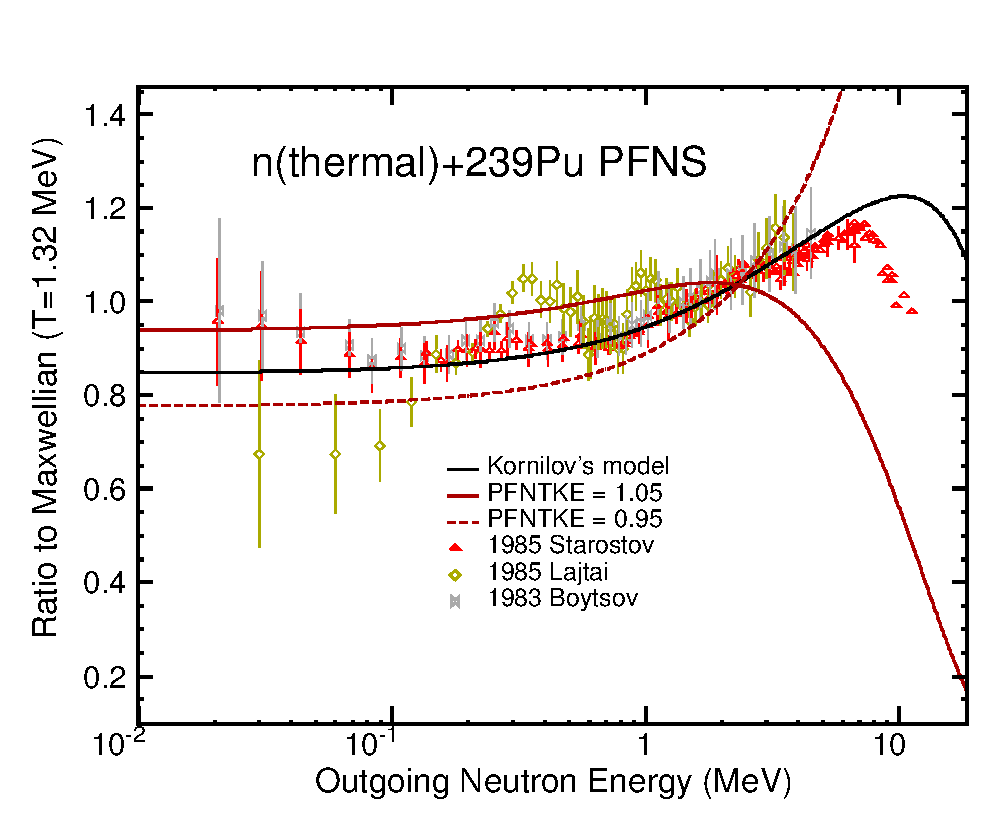
\includegraphics[width=0.8\textwidth]{figs/pfns-Edited}
\caption{Calculated prompt fission neutron spectrum for thermal neutron induced fission
on $^{239}$Pu compared with the experimental data. The effect of changing total kinetic
energy of the fragments by 5\% in both direction is shown in red. The results are
normalized to the Maxwellian distribution with $T=1.32$ MeV.}
\label{Fig-pfns}
\end{center}
\end{figure}




\part{NUCLEAR DATA EVALUATION\label{Chap:eval}}

Evaluation of nuclear data has been a major driving force in evolution of the
EMPIRE code.
EMPIRE-2.19 was extensively used in the development of the ENDF/B-VII.0
library for which it produced 78 full evaluations (nearly 20\% of the whole
neutron sublibrary). This major exercise was also a most thorough test and
validation of the system. The EMPIRE based evaluations in ENDF/B-VII.0 
can be divided into (i) fission products evaluated mostly at BNL in cooperation with KAERI, LANL, ORNL and LLNL,  (ii)
iridium isotopes evaluated by the BNL-LANL collaboration and (iii) actinides
($^{232}$Th and $^{231,233}$Pa evaluated in the frame of the IAEA
coordinated research project).  The list of fission products includes 19 
priority materials: $^{95}$Mo, $^{99}$Tc, $^{101}$Ru, $^{103}$Rh, $%
^{105}$Pd, $^{109}$Ag, $^{131}$Xe, $^{133}$Cs, $^{141}$Pr, $^{153}$Eu), $%
^{143,145}$Nd, $^{147,149,150,151,152}$Sm, and $^{155,157}$Gd. 
Nearly all evaluations cover the standard
energy range from 10$^{-5}$~eV up to 20 MeV. However, the actinide
evaluations extend up to 60 MeV proving that EMPIRE is not limited to the
classical ENDF energy range.

Recent developments focused on the covariances and resonance region. Need to produce a large number of covariances for the ENDF/B-VII.1  library was the major task that
shaped development of the code over last 6 years. In parallel, there has been necessity that a wealth of information contained in the Atlas of Neutron Resonances makes its way to the new version of the evaluated library.  This motivated development of the resonance  module of EMPIRE, which also includes covariance capabilities.  These two aspects are leading subjects of this chapter, followed by the detailed description of the method used in EMPIRE for generating exclusive spectra, recoils, details of nuclear data formatting and fitting of the optical model potential.  


\chapter{Resonance module}

\textbf{WARNING}: The module requires that electronic version of the Atlas be installed in the \emph{empire/Atlas}.  The copy rights for Atlas belong to the publisher (Elsevier), and until restrictions on its distribution are lifted most users will not be able to install  Atlas and therefore to use the resonance module of EMPIRE. 

The 3.1 version of the EMPIRE code is equipped with the module that makes use the information contained in the Atlas of Neutron Resonances~\cite{Mughabghab:06} to produce resonance files and related covariances for  the ENDF-6 formatted files.  This module facilitates  practical application of the extensive compilation of the measurements in the resonance region performed since the discovery of the neutron. 
 
The resonance module\cite{Cho2007, Herman2008} automates most of the procedures involved in evaluation 
of the resonance region. It is designed so that it can be executed within EMPIRE
or as a stand-alone program. The module reads data from the electronic version of
Atlas of Neutron Resonances, performs analysis of the available resonances,
provides statistical distributions, and computes cross sections and covariances
in the resonance region. The module also generates various plots allowing for
verification of the procedure. The resonance parameters, their uncertainties and
covariances are stored in ENDF-6 format. The formatted file can be later integrated 
into an ENDF-6 file generated by the EMPIRE code.

\section{Architecture of the module}

The module consists of the GUI script (resonance.tcl),  I/O and analysis tools
(READRP and SCANR), the processing code (THERMX), and the physics computation  codes
(PTANAL and WRIURR\cite{BNL67469}):

\begin{description}[style=multiline,leftmargin=3cm]
\item[{resonance.tcl}] graphic user interface that accepts user-supplied input,
controls the codes, plots results of statistical analysis of resonances, and compares graphically
calculated cross sections with experimental data and other evaluated nuclear data libraries
such as ENDF/B-VII.0, JEFF-3.1 and JENDL-3.3.
\item [{READRP}] reads basic physical parameters from the Atlas and RIPL.
\item[{SCANR}] performs and plots the least square fit of the resonances to determine the upper
boundary of the resolved resonance region.
\item[{THERMX}] computes cross sections for sensitivity calculations (modified version of RECENT).
\item[{PTANAL and WRIURR}] calculate Porter-Thomas distribution and write
resonance parameters in the resolved and unresolved resonance regions.
(these codes are modified with respect to the original versions to accommodate
new formulae and features, retrieve the Atlas file, and fix some bugs).
\end{description}


The module also requires experimental data in the computational format (installed in \emph{empire/EXFOR} directory), c4zvd and gnuplot for plotting, RECENT\cite{PREPRO} and SIGMA1\cite{PREPRO} codes
for cross section generation, and KALMAN, empy and some additional scripts including
addKalman.py and kalmanResonance for production of covariance matrix.
To make it functional, 'xterm' also needs to be installed.

\section{GUI control panel}

At a start-up, the module reads all the necessary data for the target nucleus including individual,
as well as average, resonance parameters from the Atlas of Neutron Resonances and RIPL
and displays them on the screen. The evaluator has the possibility to modify
the nuclear parameters before starting the calculations.
Fig.~\ref{fig:rmodule1} shows an example screen shot for Mn-55.

\begin{figure}[htbp]
\begin{centering}
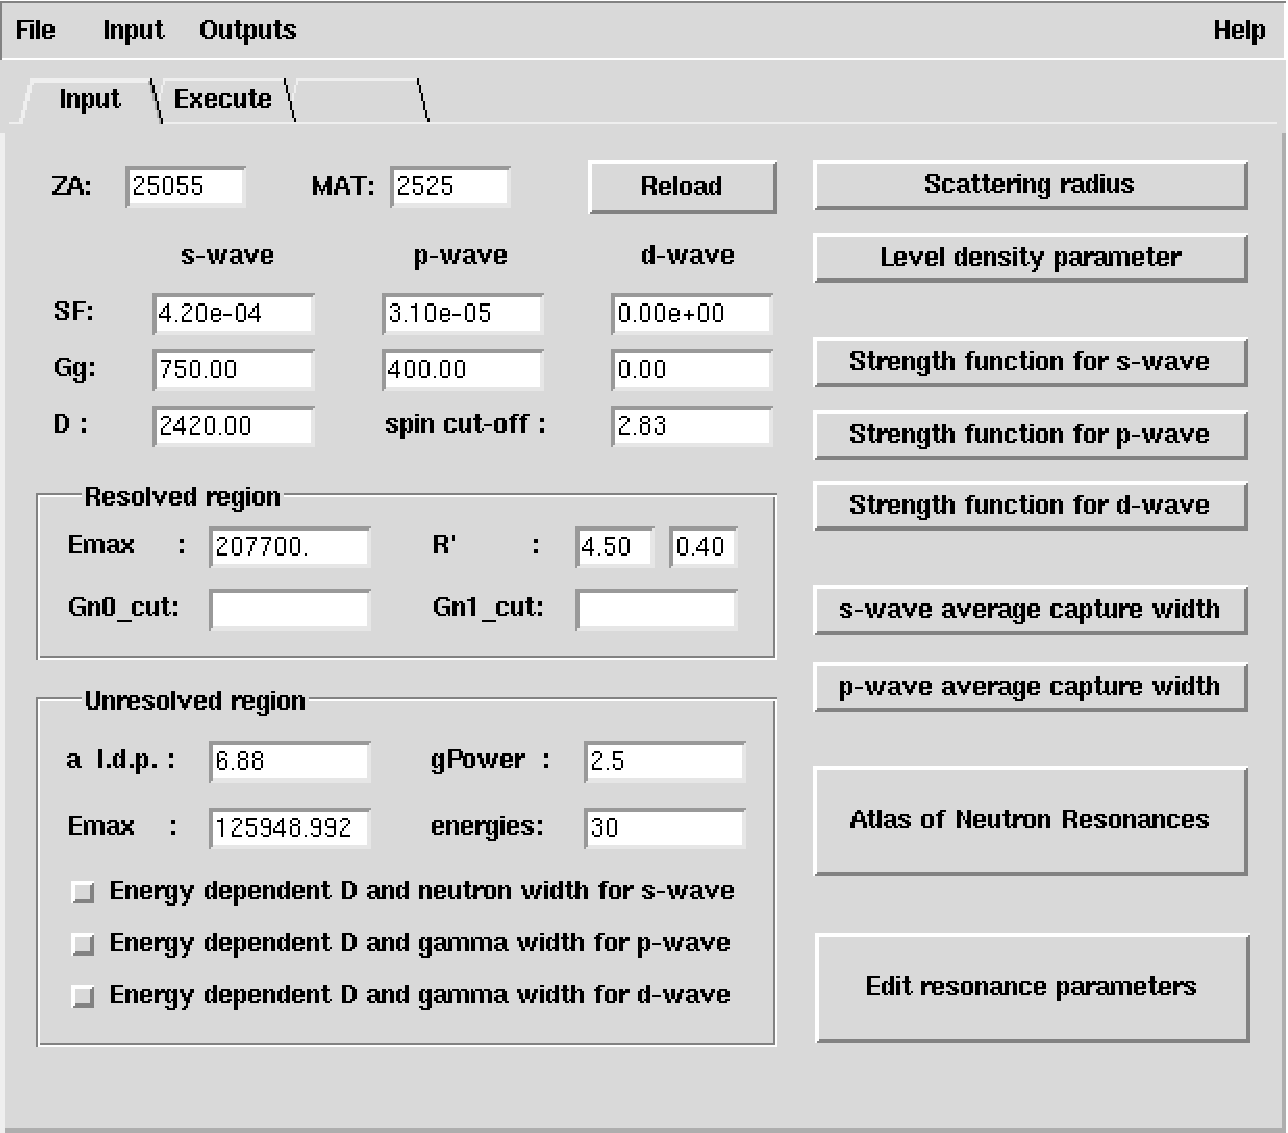
\includegraphics[width=0.7\paperwidth]{figs/rmodule1}
\caption{\label{fig:rmodule1}The screen shot of GUI main control panel (``Input'' area)}
\end{centering}
\end{figure}

The left part of the screen is the editable input area. The evaluator has a possibility to start the new
evaluation for another nuclide by entering the new ZA and MAT and then pressing the 'Reload' button.
SF, Gg, D represent the strength function, average gamma width and average level spacing, respectively.
Emax of the resolved and unresolved resonance regions is automatically calculated by retrieving the
resonance parameters from Atlas and by reading the first excited level from RIPL respectively.
In the case the $E_{max}$ of the resolved resonance region is larger than that of the unresolved region,
as  shown in Fig.~\ref{fig:rmodule1}, the module will generate a warning.

The right part of the screen provides the buttons for displaying various plots useful for the analysis of resonances.
These can be edited by clicking on the button labelled 'Edit resonance parameters'.
The modified parameter table is stored on the local directory and can be reverted to the original one
if necessary. The program for viewing the parameter tables and the one for visualizing plots can be both
customized as in the EMPIRE GUI. For a verification purpose, the  data from Atlas of Neutron
Resonances can be displayed by clicking the button labelled 'Atlas of Neutron Resonances'.

\begin{figure}[htbp]
\begin{centering}
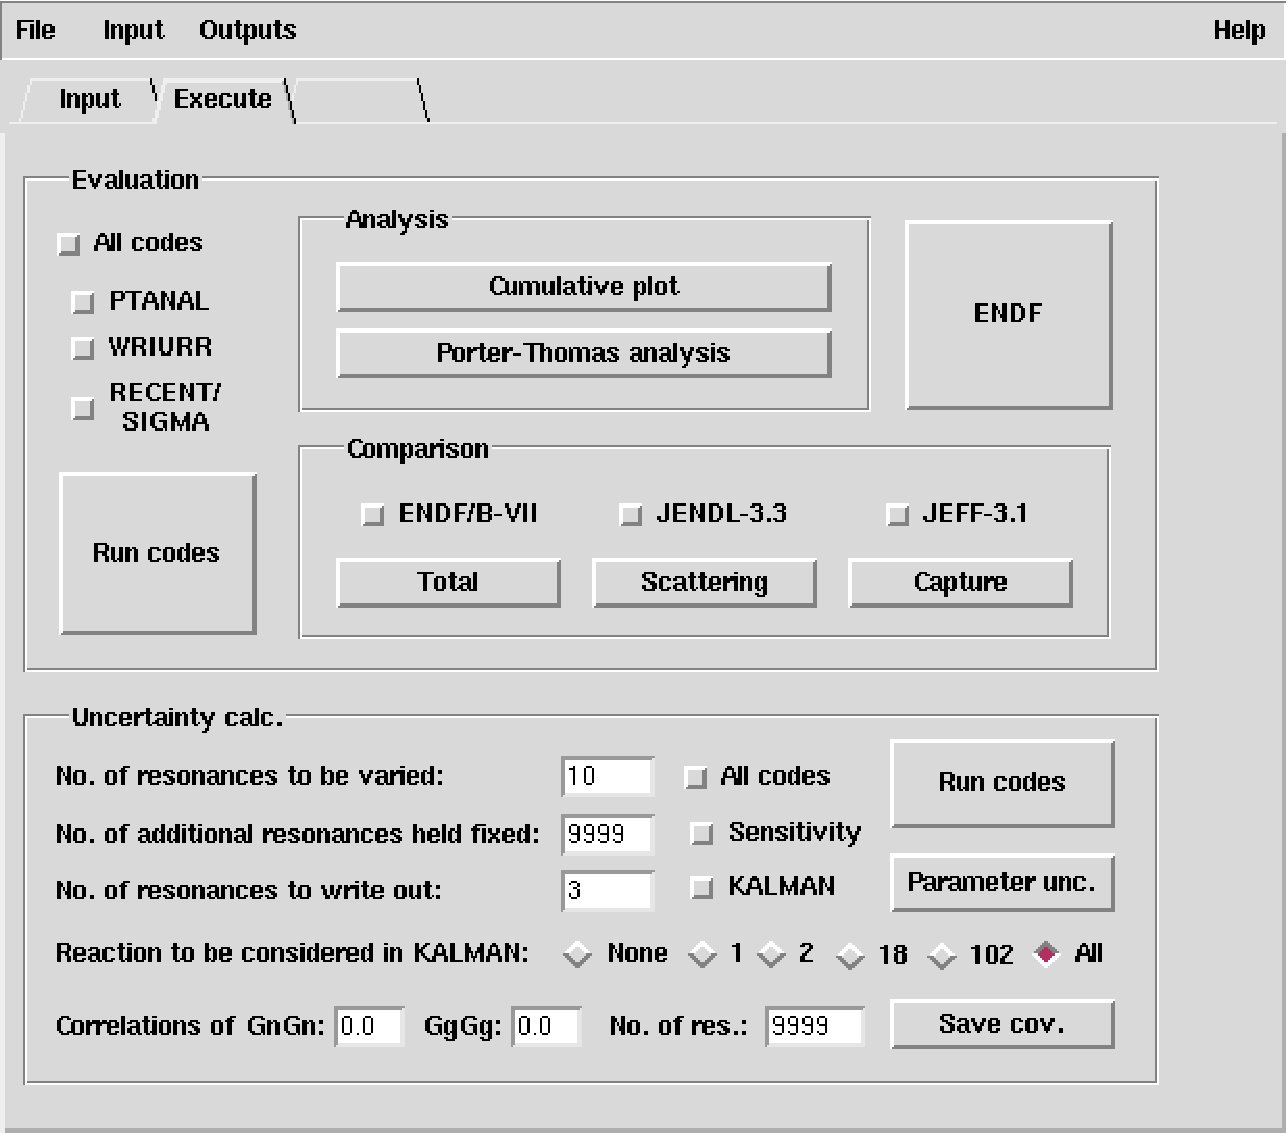
\includegraphics[width=0.7\paperwidth]{figs/rmodule2}
\caption{\label{fig:rmodule2}Screen shot of GUI main control panel (``Execute'' tab)}
\end{centering}
\end{figure}

Fig. \ref{fig:rmodule2} shows  the ``Execute'' tab of the GUI.
The upper part provide access to various codes that should be run to create ENDF-6
formatted file and point-wise cross sections. It contains also  buttons to display comparison plots of the
calculated, measured and evaluated cross sections.
The resonance parameter covariances (MF=32) can be generated using  KALMAN filter and previously calculated sensitivity matrices.  
When doing this correlations among neutron widths and among gamma widths can be supplied by the evaluator.
Resulting ENDF file including the resonance parameters and covariance matrix can be stored as a file named 
[Z*1000+A]-res.endf by clicking on the ``Save cov.'' button on the bottom of the screen.
Most tasks are performed in the background and their respective output files can be accessed through the ``Outputs'' menu on the top.

\chapter{Determination of covariances}
In recent years there has been an increasing demand from nuclear
research, industry, safety and regulatory bodies for best 
estimate predictions of system performance, such as the design and operational 
parameters of nuclear reactors, to be provided with their confidence bounds.
Estimates of the accuracy of predictions of such integral quantities  can be obtained through the 
propagation of uncertainties in evaluated microscopic neutron cross section data.

A methodology for evaluating cross section covariance data has therefore been developed within the EMPIRE code
system. The methodology covers the thermal energy, resolved resonance, unresolved
resonance and fast neutron regions and builds on the following major components:
\begin{itemize}
\item Nuclear reaction model code EMPIRE,
\item Atlas of Neutron Resonances~\cite{Mughabghab:06},
\item Kalman filter code~\cite{Kawano:97} and Monte Carlo sampling~\cite{Smith:04}.
\end{itemize}

EMPIRE provides a natural environment for implementing the covariance evaluation capabilities. 
It is built around a physics core designed for 
modeling low- to-intermediate- energy nuclear reactions. It
incorporates an extensive set of nuclear reaction models able to
describe all relevant reaction mechanisms, each of them conveniently
coupled to the up-to-date library of input model
parameters~\cite{RIPL3}. The code is also suitable for massive
calculations, is easy to use, has readily available default input
values for all parameters, and is applicable to  a wide range of
target nuclei and incident neutron energies from about 1 keV to 150 MeV.
Results may be stored in ENDF-6 format and subsequently plotted against experimental data
for verification.

The resonance module extends EMPIRE's covariance capability to the thermal and 
resonance ranges.  The module utilizes the recently published Atlas of Neutron Resonances~\cite{Mughabghab:06}, 
a monumental work by S.F. Mughabghab 
represents the 5$^{\textrm{th}}$ edition of what was previously well known as the  BNL-325 Reports. 
The resonance module contains an electronic version of these resonance parameters along with modernized versions of the legacy codes used to develop and maintain the Atlas.  In addition, the Atlas contains parameter uncertainties and the resonance module was extended to utilize this information for producing covariances in the thermal and epithermal regions.

The generation of covariances at the NNDC is based on the deterministic Kalman filter technique, which is used in the thermal and resonance range as well as in the fast neutron range. The IAEA  developers opted for the stochastic Monte Carlo (MC) procedure to generate the model-prior, coupled to the generalized least-squares code GANDR~\cite{Muir-nds:2008} to include the experimental data.
There are several fundamental and operational differences between the two methods. MC propagates uncertainties of model parameters by means of random sampling while  deterministic propagation of uncertainties, using the first-order Taylor expansion, is used in the Kalman approach. Accordingly,  higher-order effects are included in MC but not in Kalman. 
The two approaches currently also differ regarding treatment of experimental data; it is  naturally included in  Kalman whereas a  generalized least squares code GANDR must be run with the MC generated model-based prior as input.

 It is evident that both methods have their advantages and disadvantages. Availability of  
 both approaches within a single code system offers the user the choice of the appropriate method 
 for a given application.  

\section{EMPIRE-KALMAN approach}
 

In order to assess the direction of the gradient in the multi-parameter space that minimizes
$\chi^2$, the fitting code has to evaluate how much the cross sections change when a certain
parameter is varied in a given direction, i.e. the sensitivity of the cross section in respect
to each parameter variation. This information is contained in the \textit{sensitivity matrix} file. 


The Kalman filter technique is used both in the resonance and in the fast neutron region. 
It is based on minimum variance estimation and naturally combines covariances of model parameters,
of experimental data and of cross sections. This universality is a major advantage of the method.
KALMAN  uses  measurements along with their uncertainties to constrain covariances of the model
parameters via  the sensitivity matrix. Then, the final cross section covariances are calculated
from the updated covariances for model parameters.  This procedure consistently accounts  for 
the experimental uncertainties and the uncertainties of the model parameters ensuring that the
final cross section uncertainties are at least as good as the smaller of the two. We emphasize
that under the term ``reaction model'' we mean also the resonance region described by models such
as the Multi-Level Breit-Wigner formalism. 

\subsection{Sensitivity calculation}


The key ingredient of the method is the sensitivity matrix, which represents complex nuclear reaction
calculations. If we denote the combination of nuclear reaction models as an operator ${\bf \hat M}$
that transforms the vector of model parameters $\textbf{p}$ into a vector of cross sections
$\boldsymbol\sigma ({\bf p})$ for a specific reaction channel, then the sensitivity matrix ${\bf S}$
can be interpreted as the linear term in the expansion of the operator ${\bf \hat M}$,
% 
\begin{gather}
{\bf \hat M}{\bf p}= \boldsymbol\sigma({\bf p}) \nonumber\\
{\bf \hat M}({\bf p +\delta \bf p})= \boldsymbol\sigma({\bf p}) + {\bf S}\delta \bf p + \dots
\label{eq:model}
\end{gather}
\noindent 
We use `hat'  to stress that ${\bf \hat M}$ is the operator rather than a matrix.
In practice, the elements $s_{i,j}$ of the sensitivity matrix are calculated numerically as partial 
derivatives of the cross sections $\sigma$ at the energy $E_{i}$ with respect to the parameter $p_j$,
% 
\begin{equation}
s_{i,j}=\frac{\partial\sigma(E_{i},{\bf p})}{\partial p_{j}}\,.
\label{eq:sens}
\end{equation}
\noindent
 In case of covariance determination, the initial values of the parameters,
${\bf p}_{0}$, are already optimized, \textit{i.e.}, when used in
the model calculations they provide the evaluated cross sections.
Their covariance matrix ${\bf P}_{0}$ is assumed to be diagonal while
the uncertainties of the parameters are estimated using systematics,
independent measurements or educated guesses. The model-based covariance
matrix (prior) for the cross sections, ${\bf C}_{0}$, can be obtained
through a simple error propagation formula, % 
\begin{equation}
{\bf C}_{0}={\bf S}{\bf P}_{0}{\bf S}^{\textrm{T}}\,,\label{eq:mtrx}
\end{equation}
where superscript T indicates a transposed matrix.

The experimental data, if available, are included through
a sequential update of the parameter vector ${\bf p}$ and the related
covariance matrix ${\bf P}$ as 
\begin{eqnarray}
 & {\bf p}_{n+1} & ={\bf p}_{n}+{\bf P}_{n}{\bf S}^{\textrm{T}}{\bf Q}_{n+1}(\boldsymbol{\sigma}_{n+1}^{\textrm{exp}}-
      {\boldsymbol{\sigma}}({\bf p}_{n}))\nonumber \\
& {\bf P}_{n+1} & ={\bf P}_{n}-{\bf P}_{n}{\bf S}^{\textrm{T}}{\bf Q}_{n+1}{\bf S}{\bf P}_{n}\,.
\end{eqnarray}
Here, 
\begin{equation}
{\bf Q}_{n+1}=({\bf C}_{n}+{\bf C}_{n+1}^{\textrm{exp}})^{-1}\,,
\end{equation}
where $n=0,1,2,...$ and $n+1$ denotes 
update related to the sequential inclusion of the $(n+1)^{th}$ experimental
data set. In particular,  the subscript $1\equiv0+1$ denotes updating model prior ($n=0$) with the
first experiment. Vector ${\bf p}_{n+1}$ contains the improved values
of the parameters starting from the vector ${\bf p}_{n}$, and ${\bf P}_{n+1}$
is the updated covariance matrix of the parameters ${\bf p}_{n+1}$.
The ${\bf C}_{n+1}^{\textrm{exp}}$ is the cross section covariance
matrix for the $(n+1)^{\textrm{th}}$ experiment. The updated (posterior)
covariance matrix for the cross sections is obtained by replacing
${\bf P}_{0}$ with ${\bf P}_{n+1}$ in Eq.~(\ref{eq:mtrx}), % 
\begin{equation}
{\bf C}_{n+1}={\bf S}{\bf P}_{n+1}{\bf S}^{\textrm{T}}\,.\label{eq:mtrxp}
\end{equation}

\noindent The updating procedure described above is often called Bayesian,
although Eqs.~(4-\ref{eq:mtrxp}) can be derived without any reference
to the Bayes theorem.

The experimental covariance matrix, ${\bf C}_{n}^{\textrm{exp}}$,
%for the experimental data set \textit{n} 
is usually non-diagonal, due to the correlations among various energy
points $E_{i}$. Assuming that systematic experimental uncertainties
are fully correlated, % ${\bf C}_{n}^{\textrm{exp}}$
the matrix elements are expressed through the statistical, $\Delta^{\textrm{sta}}\sigma_{n}^{\textrm{exp}}$,
and systematic, $\Delta^{\textrm{sys}}\sigma_{n}^{\textrm{exp}}$,
experimental uncertainties. This yields 

\begin{equation}
{_n}c^{\textrm{exp}}_{i,i}=
% \begin{cases}
% (\Delta \sigma^{\textrm{exp,sta}}_{n}(E_i))^2+ (\Delta \sigma^{\textrm{exp,sys}}_{n}(E_i))^2       & i=k\\
% \Delta \sigma^{\textrm{exp,sys}}_{n}(E_i)\times   \Delta \sigma^{\textrm{exp,sys}}_{n}(E_k)  & i\ne k\,.
% \end{cases}
(\Delta^{\textrm{sta}} \sigma^{\textrm{exp}}_{n}(E_i))^2+
(\Delta^{\textrm{sta}} \sigma^{\textrm{exp}}_{n}(E_i))^2
\end{equation}
%
and, for $ i\ne k$, 
\begin{equation}
{_n}c^{\textrm{exp}}_{i,k}=
\Delta^{\textrm{sys}} \sigma^{\textrm{exp}}_{n}(E_i) \times 
\Delta^{\textrm{sys}} \sigma^{\textrm{exp}}_{n}(E_k)\,.
\end{equation}
%
An important  technical issue, which  has to be addressed in most of the covariance
methods,  is ensuring that the energy grid, $E_i$, for the model calculations and
experimental data is the same to enable matrix operations in Eqs.~(4-\ref{eq:mtrxp}).
In the KALMAN code this is achieved by bi-spline interpolation of model cross sections and sensitivity matrices.

The above description can easily be generalized to account for correlations among different
experiments. To this end one should construct a single vector containing all experimental
points and the related covariance matrix, which now may contain blocks correlating different
experiments. Only one  update is needed in such a case but the covariance matrices are much
bigger (in the current implementation of the Kalman filter the model-based covariance matrix
is expanded to match the experimental one).

The quality and consistency of the evaluated cross sections can be
assessed by scalar quantity 
\begin{equation}
\chi^{2}=\sum_{n=1}^{N}({\boldsymbol{\sigma}}_{n}^{\textrm{exp}} - 
{\boldsymbol{\sigma}}({\bf p}_{\textrm{N}}))^{\textrm{T}}({\bf C}_{n}^{\textrm{exp}})^{-1}
({\boldsymbol{\sigma}}_{n}^{\textrm{exp}}-{\boldsymbol{\sigma}}({\bf p}_{\textrm{N}}))\,,\label{eq:chi2}
\end{equation}
where ${\bf p}_{\textrm{N}}$ is the final set of model parameters
corresponding to the inclusion of $N$ experiments. A value of $\chi^{2}$
per degree of freedom exceeding unity indicates underestimation of
the evaluated uncertainties. It is a fairly common practice to multiply
such uncertainties by a square root of $\chi^{2}$ per degree of freedom
to address this issue.




\section{EMPIRE-MC approach}
The Monte-Carlo (MC) method is used in EMPIRE only in the fast neutron region. 
Its application to determination of covariances for the nuclear
reaction observables is very transparent~\cite{Smith:04}. First, model
input parameters that play a significant role in defining reaction
observables of interest are identified.  Then,  the EMPIRE code is run
a number of times with relevant input parameters being drawn randomly
within the assumed limits around the central (optimal) values of the
parameters. Typically, a flat distribution is used for drawing but
there is also a provision for the Gaussian one.  Each such calculation
covers the desired incident energy range and produces a full set of cross sections, spectra, angular distributions and other observables.  Standard statistical methods are used to obtain
covariances for the calculated quantities automatically including cross-reactions correlations.  The same approach can also be used for estimating cross-correlations between any two quantities. 

The MC calculations are conceptually straightforward and
free of certain simplifying assumptions, {\it e.g.}, the assumption
of a linear response of the observables to the variation of parameters,
which is inherent in the KALMAN method. There is no need for a preliminary sensitivity calculation and the computing time is independent of the employed number of model parameters. These advantages come at a price - the number of required calculations is in the range of hundreds and the convergence of the results has to be demonstrated.

The standard implementation of the MC method has no provision for incorporating experimental data. The final uncertainties and correlations depend only on the assumed uncertainties of the model parameters. These can be verified and adjusted `a posteriori'  by comparing calculated results with the spread and uncertainties of the  experimental data. However,  such verification and adjustment is subjective and lacks strict statistical justification. Nevertheless,  the model-based covariances obtained with the MC method constitute a reliable benchmark for validating faster but more approximate KALMAN calculations.
The standard implementation of the MC method has no provision for incorporating experimental data; the uncertainties and correlations depend only on the assumed uncertainties of the model parameters. However, the so-obtained covariance matrix can be used as a prior in a full analysis by the generalized least-squares method, taking experimental data and their uncertainties rigorously into account,  {\it e.g.}, the GANDR system had been used in recent IAEA evaluations.
Furthermore, the model-based covariances obtained with the MC method
constitute a reliable benchmark for validating the faster but
linear-model calculations with the KALMAN code.


\section{EMPIRE resonance covariance module}
Generation of MF32 covariances  is achieved in several steps: 
\begin{itemize}
 \item  Uncertainties for resonance parameters and thermal values  are retrieved from the electronic version of the 
Atlas. The missing information is supplied by making use of systematics or estimates. These uncertainties are put 
into an MF=32 file of resonance parameter covariances in the compact representation. This initial  matrix  is  diagonal since no correlations are provided in the Atlas. 
\item The correlations between various parameters are estimated. 
\item The resonance parameter uncertainties are adjusted so that the uncertainties of thermal values are reproduced, as discussed below.
 \end{itemize}

The resonance module has been designed to ensure consistency among thermal cross section uncertainties and uncertainties of the resonance parameters, a feature that was not addressed during the development of the Atlas database.  Thermal cross sections are usually measured with higher accuracy than resonance parameters. In order to take advantage of their superior precision while still ensuring internal consistency of the estimated covariances, we have coupled the resonance module with the Kalman filter code, which allows for an objective adjustment of the original uncertainties. 

\section{Inclusion of experimental data}
\label{sec:expdata}

\begin{figure}
\centering
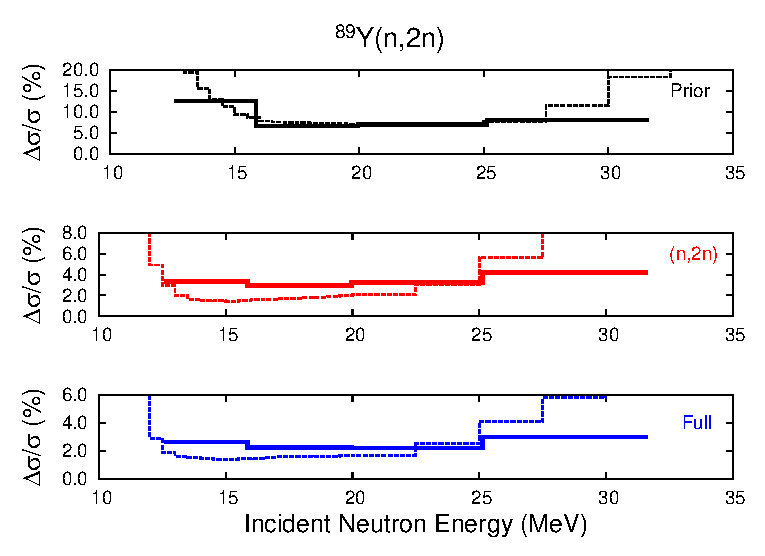
\includegraphics[width=0.7\paperwidth]{figs/plot-dcs}
\caption{Comparison of the  $^{89}$Y(n,2n) cross section uncertainties obtained with GANDR (solid lines) and KALMAN (dashed lines) illustrating inclusion of experimental data. The top panel shows the model-based uncertainties (prior), the middle panel includes (n,2n)  data only, and the bottom panel includes experimental data for all reaction channels.}
 \label{fig:kal-gandr-n2n}
\end{figure}

Inclusion of experimental data into the covariance determination still appears to be a major issue.  The KALMAN method accounts for them naturally but suffers from the general deficiency of all least squares type approaches - uncertainties tend to reach values that are considered  far too small if very many experimental data are included in the analysis.  One practical remedy to this problem is to prevent uncertainties of the model parameters to fall below some sensible limit (e.g., a systematic uncertainty of an experiment).  While this procedure, often referred as marginalization,  is simple and effective, it introduces  certain arbitrarity into the estimation of uncertainties. 

The classical formulation of the MC approach does not account for the
experimental data. Thus, in the current practice, the prior (model-based
cross section covariance), obtained with the EMPIRE-MC calculations,
was fed into the Generalized Least Squares code ZOTT  incorporated in a more general GANDR system by D.W. Muir~\cite{Muir-nds:2008}.

\section{Conclusions}
The cross section covariance capabilities of the EMPIRE code cover the full energy range relevant to applications, including thermal, resonance and fast neutron regions. This puts EMPIRE in a unique position to provide complete sets of covariance data for most of the nuclei, such as the fission products and structural materials. The code is also well capable of treating actinides.  The modules for estimating covariances for  neutron multiplicities and for fission spectra  are integrated into the EMPIRE code but need adequate parametrization.

In the fast neutron region there are two complementary methods implemented in EMPIRE for determining covariances.  The Kalman filter approach is based on variance minimization  while the stochastic one is based on the Monte Carlo sampling followed by the GANDR least-squares fitting of experimental data.  The model-based covariances obtained with the two methods are practically equivalent. There is also a possibility of using KALMAN generated model-based prior with the GANDR code. 
The Kalman filter technique is used by the resonance module of EMPIRE to impose consistency among resonance parameter uncertainties and cross section uncertainties at the thermal energy. 
In general, the KALMAN code turns out  to be  a very powerful and useful  tool for adjusting model parameters throughout the whole evaluation procedure. 

Serious concerns were raised  regarding extremely low uncertainties resulting from the least-squares analysis using model-generated priors.  These low uncertainties arise, in part, from the rigidity of the model predictions, {\it i.e.},  intrinsic model uncertainties which are not accounted for in the procedure.  Numerical experiments indicate that adding new degrees of freedom to the model has a desired effect on the output uncertainties and might be used to eliminate this deficiency.

\chapter{ENDF formatting}

One of the primary design goals of the EMPIRE code is to perform
 theoretical calculations in support of nuclear data evaluation.  To this end the code must meet certain requirements that go beyond usual features of similar codes used in pure science, e.g., calculation of nuclear recoils needed for energy balance and exclusive spectra, and ENDF-6 formatting of all calculated physical quantities, such as cross sections, spectra, angular distributions, energy-angle correlated distributions, etc.  

\section{Spectra of recoils}

Energy spectra of recoils are calculated taking into account correlations
between the excitation energy of the nucleus and the emission energy
of the particle. In order to do so, the recoil energies are followed
throughout the deexcitation cascade. A recoil spectrum is ascribed
to each excitation energy bin for each nucleus involved in the decay
chain. Emission of a particle depletes the spectrum bin of the parent
and accumulate in the recoil spectrum bin of the daughter nucleus.
$\gamma$ emissions are assumed to produce no recoil but shift respective
portions of the recoil spectrum to the the lower excitation energy
bin in the same nucleus. Transitions to discrete levels are summed
directly to the ground state recoil spectrum, since particle emission
from discrete levels is not considered and $\gamma$-emission does
not change the recoil spectrum. At the end of the decay cascade all
the recoil spectra for energy bins embedded in the continuum are null,
and the final result is given by the ground state recoil spectra.

The following assumptions are made in the course of these calculations:

\begin{itemize}
\item Particle emission from a nucleus at a certain excitation energy is
independent of the actual recoil energy of the nucleus. The center
of mass motion of a nucleus (recoil) is assumed to have no effect
on the emission of particles, as the latter involves internal degrees
of freedom. Statistically, any emission depletes the recoil spectrum
of the parent uniformly, so that for each emission the whole recoil
spectrum corresponding to the parent energy bin is reduced by a constant
factor.
\item Compound Nucleus emissions are isotropic and uncorrelated between
each other. However, forward peaked angular distributions of nucleons
emitted through the preequilibrium or direct mechanisms and the center
of mass motion of the first Compound Nucleus are retained and taken
into account in constructing recoil spectra. We note that recoils
are given in the laboratory system.
\end{itemize}
Ejectile emission energy is denoted by $\varepsilon$, excitation
energy by $E$, nucleus recoil energy by $e$, and $r$ and $p$ subscripts
are used to mark residuals and parent nuclei respectively. The $d\sigma(e,E)/de$
stands for the recoil spectrum at the excitation energy $E$ summed
over spin and parity. Consider a single emission of an ejectile with
energy $\varepsilon$; the contribution of this emission to the recoil
spectrum of the residual can be quantified. We apply momentum conservation
in binary reactions to calculate the {}``recoil kick'' energy ($\Delta e$)
for this single emission event \begin{equation}
\Delta e=\frac{m_{ejc}}{m_{r}}\varepsilon,\label{Erec}\end{equation}
in which $m_{ejc}$ and $m_{r}$ are the ejectile and recoil mass
respectively. Similarly, the contribution to the residue recoil spectrum
is obtained from the emission spectrum by applying the reverse factor\begin{equation}
\frac{d\sigma(\Delta e,E_{r})}{d(\Delta e)}=\frac{m_{r}}{m_{ejc}}\frac{d\sigma(\varepsilon,E_{r})}{d\varepsilon}.\label{CSkick}\end{equation}
The recoil energy of the residue is obtained by adding the ejectile
momentum and the momentum of the parent nucleus vectorially. We can
express the residue recoil energy $e_{r}$ through the {}``recoil
kick'' (Eq. \ref{Erec}) and the recoil energy of the parent $e_{p}$
before emission

\begin{equation}
e_{r}(e_{p},\theta)=\Delta e+e_{p}+2\sqrt{\Delta e\cdot e_{p}}\cos(\theta),\label{Eresrec}\end{equation}
 where $\theta$ is the angle between the momentum of the parent and
the {}``recoil kick''. Thus the contribution to the recoil spectrum
in the residue can be defined as \begin{equation}
\frac{d\sigma(e_{r},E_{r})}{de_{r}}=\int_{0}^{\infty}\int_{0}^{\pi}\delta\left(e_{r}-e_{r}(e_{p},\theta)\right)\left[\frac{d\sigma(e_{p},E_{p})}{de_{p}}\right]_{n}\frac{d\sigma(\Delta e,E_{r},\theta)}{d(\Delta e)}\sin(\theta)d\theta de_{p}.\label{CSrec}\end{equation}
where the $\delta$ function ensures selection of the correct recoil
energy and the square brackets $\left[\right]_{n}$ around the parent
recoil spectrum indicate that the integral was normalized to unity:\begin{equation}
\int_{0}^{\infty}\frac{d\sigma(e_{p},E_{p})}{de_{p}}de_{p}=1.\end{equation}
Integration in Eq. \ref{CSrec} is limited by the range of possible
recoil energies. We note that Eq. \ref{CSrec} distributes the recoil
cross section related to a single emission event over various recoil
energies. The reason for this spread is two-fold: (i) vectorial coupling
of momenta and (ii) recoil spectrum of the parent nucleus. Even in
the case of a delta-function parent spectrum (the first CN), the residual
spectrum covers the range from $\Delta e+e_{p}-2\sqrt{\Delta e\cdot e_{p}}$
to $\Delta e+e_{p}+2\sqrt{\Delta e\cdot e_{p}}$ , as results from
Eq. \ref{Eresrec}. The $d\sigma(\Delta e,E_{r},\theta)/d(\Delta e)$
is assumed to be isotropic ($\theta$ independent) except for the
MSD\index{MSD} and direct inelastic contributions, for which angular
distributions are preserved in Eq. \ref{CSrec}. The recoil spectrum
of the Compound Nucleus is single valued and differs from zero only
at the energy of the Center of Mass motion. This is also the first-parent
spectrum to which Eq. \ref{CSrec} is sequentially applied. We note
that Eq. \ref{CSrec} refers to the emissions of a single type ejectile
with a given emission energy. Eq. \ref{CSrec} is  applied to all
possible emissions including summation over different ejectile types
and parent/residue excitation energies. 


\section{Exclusive spectra}

EMPIRE may rearrange emission spectra to conform to the ENDF representation,
which require that for a given reaction all pertinent subsequent emissions
are summed up to produce effective spectra (for each ejectile) associated
with the reaction. For example, neutron spectrum from the (n,2n) reaction
should contain a sequence of two neutron emissions, which is followed
by the $\gamma$-cascade only. Thus the contribution of the first
neutron should be subtracted from the (n,n) and added to the (n,2n)
spectrum. 

A new algorithm for calculation of the exclusive spectra has been
developed and implemented in EMPIRE-3.1. It is based on the concept
of the 'population spectra', also used for the recoils, and avoids
approximations inherent in the previous method. The new algorithm
is more precise, never produces negative cross sections, and can treat
an arbitrary number of emissions.

We want to calculate the populations and exclusive cross sections
obtained from the statistical decay of nuclei remaining after a series
of direct/pre-equilibrium reactions. We represent the properties of
a nuclear state as $\alpha=(E_{\alpha}^{*},\, I_{\alpha},\,\pi_{\alpha},\, Z_{\alpha},\, A_{\alpha})$
and that of an ejectile as $\beta=(e_{\beta},\, j_{\beta},\, l_{\beta},\, z_{\beta},\, a_{\beta})$.
That is, we assume a complete description of a nuclear state, in terms
of excitation energy, angular momentum, parity and charge and mass
numbers, and of the emitted particle, in terms of emission energy,
total and orbital angular momenta and charge and mass numbers. We
do not take gamma emission into account. We write the differential
occupation spectrum, that is, the differential (in energy) cross section/occupation
of the state $\alpha$, as $POP(\alpha)$, with the initial spectrum
obtained from the absorption/direct reaction as $POP_{0}(\alpha)$.
We can determine the differential occupation of a given state by following
the decay chain. In terms of the predecessors $\alpha^{\prime}$ of
the nucleus in question, we can write\[
POP(\alpha)=\sum_{\alpha\prime,\beta}\Pi(\alpha,\alpha^{\prime};\beta)\, POP(\alpha^{\prime})+POP_{0}(\alpha)\,,\]
where $\Pi(\alpha,\alpha^{\prime};\beta)$ is the usual Hauser-Feshbach
transition element,\[
\Pi(\alpha,\alpha^{\prime};\beta)=\frac{\rho(E_{\alpha}^{*},I_{\alpha},\pi_{\alpha})\tau_{c}(I_{\alpha},\pi_{\alpha},I_{\alpha^{\prime}},\pi_{\alpha^{\prime}},e_{\beta},j_{\beta},l_{\beta})}{\sum_{\tilde{\beta},I_{\tilde{\alpha}},\pi_{\tilde{\alpha}}}\int de_{\tilde{\beta}}\:\rho(E_{\tilde{\alpha}}^{*},I_{\tilde{\alpha}},\pi_{\tilde{\alpha}})\tau_{\tilde{\beta}}(I_{\tilde{\alpha}},\pi_{\tilde{\alpha}},I_{\alpha^{\prime}},\pi_{\alpha^{\prime}},e_{\tilde{\beta}},j_{\tilde{\beta}},l_{\tilde{\beta}})}\]
 where $\rho(E_{\alpha}^{*},I_{\alpha},\pi_{\alpha})$ is the density
of states of the residual nucleus of spin $I_{\alpha}$, parity $\pi_{\alpha}$
and excitation energy $E_{\alpha}^{*}=E_{\alpha^{\prime}}^{*}-B_{\beta}-e_{\beta}$,
with $E_{\alpha^{\prime}}^{*}$ the excitation energy of the initial
compound nucleus and $B_{\beta}$ the separation energy of the emitted
particle $\beta$. We assume that the transmission factor
$\tau_{\beta}(I_{\alpha},\pi_{\alpha},I_{\alpha^{\prime}},\pi_{\alpha^{\prime}},e_{\beta},j_{\beta},l_{\beta})$
can be written in terms of the spherical optical model transmission
coefficients in channel $\beta$, $T_{\beta}^{j_{\beta}l_{\beta}}(e_{\beta})$.
It takes the form \[
\tau_{\beta}(I_{\alpha},\pi_{\alpha},I_{\alpha^{\prime}},\pi_{\alpha^{\prime}},e_{\beta},j_{\beta},l_{\beta})=\frac{(1+(-1)^{l_{\beta}}\pi_{\alpha}\pi_{\alpha^{\prime}})}{2}T_{\beta}^{j_{\beta}l_{\beta}}(\varepsilon_{\beta})\,,\]
 where the factor in parentheses ensures that parity is conserved. 

We can simplify these expressions slightly by including the sums over
the angular momentum of the emitted particle in the transmission factor.
We write\[
POP(\alpha)=\sum_{\alpha\prime,\beta}\Pi(\alpha,\alpha^{\prime};\bar{\beta})\, POP(\alpha^{\prime})+POP_{0}(\alpha)\,,\]
with \[
\Pi(\alpha,\alpha^{\prime};\bar{\beta})=\frac{\rho(E_{\alpha}^{*},I_{\alpha},\pi_{\alpha})\tau_{c}(I_{\alpha},\pi_{\alpha},I_{\alpha^{\prime}},\pi_{\alpha^{\prime}},e_{\beta})}{\sum_{\tilde{\beta},I_{\tilde{\alpha}},\pi_{\tilde{\alpha}}}\int de_{\tilde{\beta}}\:\rho(E_{\tilde{\alpha}}^{*},I_{\tilde{\alpha}},\pi_{\tilde{\alpha}})\tau_{\tilde{\beta}}(I_{\tilde{\alpha}},\pi_{\tilde{\alpha}},I_{\alpha^{\prime}},\pi_{\alpha^{\prime}},e_{\tilde{\beta}})}\,,\]
and $\bar{\beta}=(e_{\beta},\, z_{\beta},\, a_{\beta})$, where we
now have \[
\tau_{\beta}(I_{\alpha},\pi_{\alpha},I_{\alpha^{\prime}},\pi_{\alpha^{\prime}},e_{\beta})=\sum_{j=|I_{\alpha}-I_{\alpha^{\prime}}|}^{I_{\alpha}+I_{\alpha^{\prime}}}\sum_{l=|j-s_{\beta}|}^{j+s_{\beta}}\frac{(1+(-1)^{l}\pi_{\alpha}\pi_{\alpha^{\prime}})}{2}T_{\beta}^{jl}(\varepsilon_{\beta})\,,\]
after taking into account angular momentum conservation when defining
the sums.

We also wish to calculate exclusive cross sections, which we define
as the double differential cross section/occupation for obtaining
a nucleus in the state $\alpha$ after emitting a particle $\beta$.
This cross section, which we write as $POPcse(\alpha,\,\beta)$, takes
into account all emissions of a particle $\beta$ that lead to the
final state $\alpha$. By following the decay chain, the exclusive
cross section $POPcse(\alpha,\,\beta)$ can be obtained as, \begin{eqnarray*}
POPcse(\alpha,\beta) & = & \sum_{\alpha^{\prime}}\Pi\left(\alpha,\alpha^{\prime};\beta\right)POP\left(\alpha^{\prime}\right)+POPcse_{0}(\alpha,\beta)\\
 &  & \qquad\qquad+\sum_{\alpha^{\prime}\beta^{\prime}}\Pi\left(\alpha,\alpha^{\prime};\beta^{\prime}\right)POPcse\left(\alpha^{\prime},\beta\right)\,,\end{eqnarray*}
where $POPcse_{0}(\alpha,\beta)$ is the contribution of the absorption/direct
reaction. The expression for the exclusive cross section has two additional
terms. The first is just that of a transition to $\alpha$ through
emission of the particle $\beta$, which is proportional to the transition
element $\Pi\left(\alpha,\alpha^{\prime};\beta\right)$. The second
is the contribution from all anterior emissions of a particle $\beta$
that, in the last transition, lead to the state $\alpha$. This can
be written in terms of the exclusive cross sections of the predecessors,
$POPcse\left(\alpha^{\prime},\beta\right)$. 

We can immediately sum over the emitted particle angular momenta,
$j_{\beta}$ and $l_{\beta}$, to write the equation defining the
exclusive cross section as \begin{eqnarray*}
POPcse(\alpha,\bar{\beta}) & = & \sum_{\alpha^{\prime}}\Pi\left(\alpha,\alpha^{\prime};\bar{\beta}\right)POP\left(\alpha^{\prime}\right)+POPcse_{0}(\alpha,\bar{\beta})\\
 &  & \qquad\qquad+\sum_{\alpha^{\prime}\bar{\beta}^{\prime}}\Pi\left(\alpha,\alpha^{\prime};\bar{\beta}^{\prime}\right)POPcse\left(\alpha^{\prime},\bar{\beta}\right)\,.\end{eqnarray*}
Ideally, we would also like to obtain expressions summed over $I_{\alpha}$ and
$\pi_{\alpha}$ for both $POP(\alpha)$ and $POPcse(\alpha,\bar{\beta})$.
However, for this to be possible, the summed transition element\[
\Pi(\bar{\alpha},\alpha^{\prime};\bar{\beta})=\frac{\sum_{I_{\alpha},\pi_{\alpha}}\rho(E_{\alpha}^{*},I_{\alpha},\pi_{\alpha})\tau_{c}(I_{\alpha},\pi_{\alpha},I_{\alpha^{\prime}},\pi_{\alpha^{\prime}},e_{\beta})}{\sum_{\tilde{\beta},I_{\tilde{\alpha}},\pi_{\tilde{\alpha}}}\int de_{\tilde{\beta}}\:\rho(E_{\tilde{\alpha}}^{*},I_{\tilde{\alpha}},\pi_{\tilde{\alpha}})\tau_{\tilde{\beta}}(I_{\tilde{\alpha}},\pi_{\tilde{\alpha}},I_{\alpha^{\prime}},\pi_{\alpha^{\prime}},e_{\tilde{\beta}})}\]
would have to be independent of $I_{\alpha^{\prime}}$ and $\pi_{\alpha^{\prime}}$.
In general, this is not the case, so that the general equations should
be used. In EMPIRE, the general equation is used to determine $POP(\alpha)$
but not $POPcse(\alpha,\bar{\beta}$). In particular, the angular
momentum dependence of the $POPcse(\alpha^{\prime},\bar{\beta}$)
contributions to $POPcse(\alpha,\bar{\beta}$) are neglected. We could easily avoid this approximation but calculation time would grow by orders of magnitude  - the increase that would not be justified by more precise splitting of inclusive spectra into its exclusive components.

When the angular momentum dependence can be neglected, the expressions
reduce to Weisskopf-Ewing ones. This is possible when we can approximate
the density of states as\[
\rho(E_{\alpha}^{*},I_{\alpha},\pi_{\alpha})\approx\frac{1}{2}\rho(E_{\alpha}^{*},I_{\alpha})\approx\frac{1}{2}(2I_{\alpha}+1)\rho(E_{\alpha}^{*},0)\]
for the states occupied in the reaction. It is then possible to reduce
the summed transition element to \[
\Pi(\bar{\alpha},\alpha^{\prime};\bar{\beta})=\frac{(2s_{\beta}+1)\mu_{\beta}\varepsilon_{\beta}\sigma_{\beta}(\varepsilon_{\beta})\rho(E_{\alpha}^{*},0)}{\sum_{\tilde{\alpha}\tilde{\beta}}\int d\varepsilon_{\tilde{\beta}}\:(2s_{\tilde{\beta}}+1)\mu_{\tilde{\beta}}\varepsilon_{\tilde{\beta}}\sigma_{\tilde{\beta}}(\varepsilon_{\tilde{\beta}})\rho(E_{\tilde{\alpha}}^{*},0)}\]
and write the summed equations as\[
POP(\bar{\alpha})=\sum_{\alpha\prime,\beta}\Pi(\bar{\alpha},\alpha^{\prime};\bar{\beta})\, POP(\bar{\alpha}^{\prime})+POP_{0}(\bar{\alpha})\]
and \begin{eqnarray*}
POPcse(\bar{\alpha},\bar{\beta}) & = & \sum_{\alpha^{\prime}}\Pi\left(\bar{\alpha},\alpha^{\prime};\bar{\beta}\right)POP\left(\bar{\alpha}^{\prime}\right)+POPcse_{0}(\bar{\alpha},\bar{\beta})\\
 &  & \qquad\qquad+\sum_{\alpha^{\prime}\bar{\beta}^{\prime}}\Pi\left(\bar{\alpha},\alpha^{\prime};\bar{\beta}^{\prime}\right)POPcse\left(\bar{\alpha}^{\prime},\bar{\beta}\right)\,.\end{eqnarray*}

In EMPIRE, the general equation maintaining the full angular momentum
dependence is used to determine $POP(\alpha)$ but not $POPcse(\alpha,\bar{\beta}$).
The angular momentum summed forms of the exclusive cross sections,
$POPcse(\bar{\alpha},\bar{\beta})$, are approximated as \begin{eqnarray}
POPcse(\bar{\alpha},\bar{\beta}) & = & \sum_{\alpha^{\prime}}\Pi\left(\bar{\alpha},\alpha^{\prime};\bar{\beta}\right)POP\left(\alpha^{\prime}\right)+POPcse_{0}(\bar{\alpha},\bar{\beta})\\
 &  & \qquad\qquad+\sum_{\bar{\alpha}^{\prime}\bar{\beta}^{\prime}}\hat{\Pi}\left(\bar{\alpha},\bar{\alpha}^{\prime};\bar{\beta}^{\prime}\right)POPcse\left(\bar{\alpha}^{\prime},\bar{\beta}\right)\nonumber \\
 & = & \sum_{\bar{\alpha}^{\prime}}\hat{\Pi}\left(\bar{\alpha},\bar{\alpha}^{\prime};\bar{\beta}\right)POP\left(\bar{\alpha}^{\prime}\right)+POPcse_{0}(\bar{\alpha},\bar{\beta})\nonumber \\
 &  & \qquad\qquad+\sum_{\bar{\alpha}^{\prime}\bar{\beta}^{\prime}}\hat{\Pi}\left(\bar{\alpha},\bar{\alpha}^{\prime};\bar{\beta}^{\prime}\right)POPcse\left(\bar{\alpha}^{\prime},\bar{\beta}\right)\,,\nonumber \end{eqnarray}
where the effective transition matrix element is approximated using
the angular momentum dependence of the decaying population, \begin{equation}
\hat{\Pi}\left(\bar{\alpha},\bar{\alpha}^{\prime};\bar{\beta}^{\prime}\right)=\frac{1}{POP\left(\bar{\alpha}^{\prime}\right)}\sum_{I_{\alpha^{\prime}}\pi_{\alpha^{\prime}}}\Pi\left(\bar{\alpha},\alpha^{\prime};\bar{\beta}\right)POP\left(\alpha^{\prime}\right)\,.\end{equation}
 Note that this reduces to the Weisskopf-Ewing transition matrix element
when $\Pi\left(\bar{\alpha},\alpha^{\prime};\bar{\beta}\right)$ is
independent of the spin and parity, $I_{\alpha^{\prime}}$ and $\pi_{\alpha^{\prime}}$,
of the decaying nucleus.

The same approximation is used to calculate the exclusive angular
distributions, with the additional assumption that the angular dependence
arises from the direct / absorption contributions to the reaction,
$POPcse_{0}(\bar{\alpha},\bar{\beta})$. An exclusive angular distribution
involving the emission of $n$ particles will thus have contributions
from one direct emission followed by $n-1$ statistical emissions,
from either of two direct emissions followed by $n-2$ statistical
emissions, etc., up to any of $n-1$ direct
emissions followed by one statistical emission and, finally, a contribution
from any of $n$ direct emissions. 

Let us denote the exclusive angular distribution of particle $\bar{\beta}$
at angle $\theta$ to form the residue $\bar{\alpha}$ as $POPcse\left(\bar{\alpha},\bar{\beta},\theta\right)$
with the initial direct contribution written analogously as $POPcse_{0}\left(\bar{\alpha},\bar{\beta},\theta\right)$.
Taking into account the considerations above, we can write an approximate
equation for the angular distribution as \begin{eqnarray}
POPcse(\bar{\alpha},\bar{\beta},\theta) & =\frac{1}{4\pi} & \sum_{\bar{\alpha}^{\prime}}\hat{\Pi}\left(\bar{\alpha},\bar{\alpha}^{\prime};\bar{\beta}\right)POP\left(\bar{\alpha}^{\prime}\right)+POPcse_{0}(\bar{\alpha},\bar{\beta},\theta)\\
 &  & \qquad\qquad+\sum_{\bar{\alpha}^{\prime}\bar{\beta}^{\prime}}\hat{\Pi}\left(\bar{\alpha},\bar{\alpha}^{\prime};\bar{\beta}^{\prime}\right)POPcse\left(\bar{\alpha}^{\prime},\bar{\beta},\theta\right)\,.\nonumber\end{eqnarray}
The total direct reaction contribution can be isolated as $POPcse_{d}(\bar{\alpha},\bar{\beta},\theta)$
with\begin{equation}
POPcse_{d}(\bar{\alpha},\bar{\beta},\theta)=\sum_{\bar{\alpha}^{\prime}\bar{\beta}^{\prime}}\hat{\Pi}\left(\bar{\alpha},\bar{\alpha}^{\prime};\bar{\beta}^{\prime}\right)POPcse_{d}\left(\bar{\alpha}^{\prime},\bar{\beta},\theta\right)+POPcse_{0}(\bar{\alpha},\bar{\beta},\theta)\,.\end{equation}
For a single emission, EMPIRE calculates this as \begin{equation}
POPcse_{d}(\bar{\alpha},\bar{\beta},\theta)=\sum_{\bar{\alpha}^{\prime}}\, POPcseaf\left(\bar{\alpha},\bar{\alpha}^{\prime},\bar{\beta}\right)POPcse_{0}(\bar{\alpha}^{\prime},\bar{\beta},\theta)\,,\end{equation}
where \begin{equation}
POPcseaf\left(\bar{\alpha},\bar{\alpha},\bar{\beta}\right)=1.\end{equation}
However, in this case the representation of $POPcseaf\left(\bar{\alpha},\bar{\alpha}^{\prime},\bar{\beta}\right)$
is greatly simplified as the energy of the first residual CN is completely
correlated with that of the emitted particle, so that only two energy
indices are needed to represent 
$POPcseaf\left(\bar{\alpha},\bar{\alpha}^{\prime},\bar{\beta}\right)$,
those of $\bar{\alpha}$ and $\bar{\beta}$.
For second and higher emissions this is no longer the case.
When all three energy indices are needed, it is more convenient
to calculate $POPcse_{d}(\bar{\alpha},\bar{\beta},\theta)$ directly.


\section{EMPEND code }

The ENDF formatted file is created by the user selecting the ENDF
option in the input file ({*}.\emph{inp}). This instructs EMPIRE to
write all necessary information to the output file \emph{{*}.out},
which may actually become very long, depending to some extent on the
choice of input options in the EMPIRE calculations. This file is
processed by the utility code EMPEND\index{EMPEND} written by Trkov, 
which creates the ENDF-6 formatted file.

EMPIRE provides inclusive cross sections for production of the residues, i.e., all paths to the final nucleus are summed  together (e.g., (n,np)+(n,pn)+(n,d)). Only for the reactions involving emission of a single type of particle the reaction cross sections are exclusive (e.g., (n,n), (n,2n), (n,3n), ... or (n,p), (2p),...). As described in the previous section, user may request inclusive or exclusive particle  and gamma emission spectra.  Employing a rather involved bookkeeping, EMPIRE can keep track of the sequential decays to produce spectra associated with the particular residue.  User may choose how many emissions are treated in the exclusive approach. The remaining emissions are inclusive, i.e., rather than providing exclusive cross sections and associated spectra for each of the reactions separately, EMPIRE can output
inclusive cross sections, spectra and double-differential cross sections.
This means that the total emission spectra of neutrons, protons, 
$\alpha$-particles and $\gamma$s are printed, instead of individual 
contributions from the reactions, with the exception of some distinct
reactions that are always treated exclusively 
(e.g. inelastic, (n,2n), (n,p), etc.) 
This is the preferred mode of EMPIRE execution
when ENDF formatting is required. EMPEND\index{EMPEND} automatically 
recognizes the calculation options from the contents and acts accordingly.

EMPIRE also calculates cross sections for the production of metastable
isomers. EMPEND recognizes these and stores them in ENDF File~10.
Cross sections for radionuclide production, which can not be uniquely
associated with any specific reaction (i.e. an ENDF MT number) are
lumped into File~3 MT~5, but to preserve the complete information, the
radionuclide production is stored in File~10, MT~5. This can be done 
because according to ENDF-6 rules the cross sections in File~10 by
definition are not required for the reconstruction of redundant reactions.

The ENDF file has to obey the rules of sorting the data in increasing order
by data type (MF number) and reaction type (MT number),
so several sweeps of the EMPIRE output file must be made, which may
slow down the formatting process considerably. In general, the
required operations are described as follows:

\begin{itemize}
\item In the first sweep the cross sections and the corresponding             
   reaction Q-values are extracted. All reading is done with               
   the REAMF3 routine.                                                     
\item In the next sweep all reactions for which particle spectra              
   are given are identified. All reading is done with the SCNMF6           
   routine.                                                                
\item Another sweep is made for each reaction having angular                  
   distributions. This applies to the elastic and all discrete             
   level reactions (inelastic neutron, alpha and proton                    
   emission).                                                              
\item Next follows a sweep for each reaction having energy-angle              
   correlated outgoing particle distributions.                             
\item Finally, a sweep is made for the remaining reactions,                   
   particularly the (n,$\gamma$) reaction, for which the                      
   particle distributions are coded in ENDF File-6.                        
\end{itemize}
                                                                           
In the first sweep radionuclide production cross sections are              
located and the MT numbers are assigned, when possible.                    
Cross sections, which can not be identified uniquely by an MT              
number are assigned MT=10(Z*1000+A)+LFS where LFS is the final             
isomeric state of the nuclide. The spin of the target nucleus,             
the S$_0$-strength function, the average gamma width, the average             
level spacing and the energy-dependent scattering radius are               
also extracted to enable the assembly of the dummy resonance               
parameter file.                                                            

  In the second sweep, all reactions that do not have explicitly           
given spectra are identified. When many exclusive spectra are           
requested in the EMPIRE calculation, there may be cases where              
particle spectra are given but no MT number is assigned. The               
spectra are ignored, the cross sections are added to MT=5 and              
particle production cross sections for this MT are incremented.
This preserves particle multiplicities, but spectral shapes may 
become distorted.
  After the second sweep, all necessary information is                     
available to write the comments-section (MF=1) and the prompt              
nu-bar (if the nuclide is fissile). For incident neutrons a                
dummy resonance file (File~2) is constructed.                                
  The cross section data found on the file are fitted by a                 
cubic spline and entered into the output ENDF file on a                    
user-defined dense energy grid, thinned to the specified                   
tolerance and taking reaction thresholds into account.                     
If desired, the spline interpolation may be suppressed and                 
the energy points found on the file are entered directly into              
the ENDF formatted file.                                                   
                                                                           
The angular distributions for discrete level reactions                     
that appear in the ENDF File~4 sections are extracted from                 
the spectra on the EMPIRE output file, interpolated to                     
the appropriate energy, if necessary. Legendre polynomial                  
coefficients in the centre-of-mass are fitted to the                       
distributions. For elastic scattering the Legendre                         
coefficients are copied directly from the EMPIRE output;                   
If more than 64 Legendre coefficients are required, formatting             
switches automatically to pointwise representation.                        
                                                                           
The correlated energy-angle distributions for continuum                    
reactions that appear in ENDF File-6 sections are entered                  
in Legendre polynomial representation in the centre-of-                    
mass coordinate system. The maximum Legendre order is                      
limited to 64. For reactions with relatively smooth                        
angular distributions, the number of coefficients is                       
reduced accordingly.                                                       
                                                                           
Photon production information for discrete levels can be stored            
in ENDF Files~12 and 14. The spectra for the continuum are                 
included in File-6 (rather than File~15). File~12 contains photon          
transition probabilities and photon emission probabilities for             
discrete level reactions, while File~14 contains the corresponding         
angular distributions, which are assumed isotropic. The gamma              
spectra of the (n,gamma) reaction are presently stored in File-6.          
Primary gammas, which are optionally printed in the Empire output          
explicitly are not formatted. This option should not be used when 
ENDF formatting is required. By default, primary gammas are included
in the photon spectrum in tabular form.
                                                                           
\section{EMPEND Input instructions}

The program can be executed interactively from a terminal                  
screen. The required input is entered in response to the                   
prompts, which are the following:                                          
\begin{itemize}
\item The name of the EMPIRE output file to be processed.                     
\item The name of the ENDF formatted file to be written.                      
\item Number of subintervals per incident neutron energy interval             
   on the EMPIRE output file. The subintervals define the fine             
   energy mesh for the cross sections on the ENDF formatted                
   file. The following are applicable:                                     
   \begin{itemize}
     \item[0]  Only the points on the EMPIRE output are entered to the            
        ENDF formatted file.                                               
     \item[1]  The points at reaction thresholds are added. The energy          
        points above threshold are as found in the EMPIRE output file.               
     \item[n]  Threshold points are entered, but in addition, each                
        interval on the EMPIRE output is subdivided into ``n''               
        subintervals. Cross section values at intermediate points          
        are defined by a cubic spline fit.                                 
   \end{itemize}
\item Thinning tolerance limit [\%] to reduce the number of cross              
   section points. Data points, which can be reproduced from the           
   neighboring points by linear interpolation to within the               
   specified tolerance, are removed. Entering a negative value             
   for the thinning tolerance limit causes thinning to be                  
   suppressed.                                                             
\item ENDF material number identifier.                                        
\item NLIB number assigned to the evaluation (see ENDF-6 manual).             
   The parameter is optional.                                            
\item ALAB, EDATE, AUTHOR string, where each of the listed                    
   parameters occupies 11 columns (see ENDF-6 manual for                   
   details). The parameters are optional.                                  
\end{itemize}
                                                                           
NOTES:                                                                    
\begin{itemize}
\item Extensive exclusive spectra calculations in EMPIRE                      
   should be avoided when ENDF formatting is needed, since                 
   for complex reactions when a residual nuclide can be                    
   produced from more than one reaction, the assignment of                 
   spectra can not be done uniquely. It is recommended to                  
   allow up to 4 emitted neutrons and only a single charged                
   particle.                                                               
\item All text preceding the printout for first energy is                    
   transferred to the comments section in the ENDF file (FM=1,             
   MT=451). The easiest way to insert customized comments into             
   the ENDF file is to modify (manually) the EMPIRE output.                
\item The resonance file (MF=2) that is generated for files                   
   with incident neutrons is by no means a realistic cross                 
   section representation. It is given for completeness, when              
   no information on the resonances (other than from the                   
   systematics is available). The code places resonances spaced            
   uniformly around the thermal value according to the given               
   average level spacing. The neutron width is defined from the            
   S0 strength function and the gamma-widths are the average               
   gamma widths. The assigned resonance formalism is the                   
   Multi-level Breit-Wigner formalism with energy-dependent                
   scattering radius.                                                      
\end{itemize}
                                                                           
To monitor the formatting process for quality assurance                    
purposes, the EMPEND.LOG file is written in which the                      
details of the formatting process are recorded. A limited                  
amount of checking is done. An entry to the log file is                    
added in the following cases:                                               
\begin{itemize}
\item The cross section obtained by integrating the spectrum                  
   should agree with the value given directly in the                       
   EMPIRE output file. If the difference exceeds 2\%,                       
   a warning message is written, giving the reaction                       
   MT number, the incident particle energy, the expected                   
   cross section (i.e. the value given directly in the                     
   EMPIRE output file) and the percent difference.                         
\item The angular distributions are fitted to determine the                   
   Legendre polynomial expansion coefficients. If the                      
   distribution reconstructed from the Legendre polynomial                 
   coefficients differs from the pointwise values on the                   
   EMPIRE output file by more than 5\%, a warning message                   
   is written, giving the reaction MT number, the outgoing                 
   particle ZA identifier, the incident and the outgoing                   
   particle energies and the percent difference in the                     
   fitted distribution from the pointwise value on the                     
   file.                                                                   
\end{itemize}
Additional messages monitor the progress of the data                       
formatting process.                                                        




\chapter{Nuclear astrophysics\label{Chap:S-FACTOR}}

Although EMPIRE is a model code used primarily for nuclear data evaluation, it has the inherent capabilities to be used as a nuclear reaction model code for nuclear astrophysics applications.  In that vein, the S-factor has been implemented into the EMPIRE code.  The formalism that follows is valid for nonresonant reactions only \cite{iliadis:07} \cite{RR}.

The S-factor removes the barrier penetrability (s-wave transmission probablility) and the 1/$E$ dependence of the cross section.  It is generally expressed as:

\begin{equation}
S(E)=\sigma(E) E \exp[2\pi\eta]
\end{equation}
where $\sigma(E)$ is the cross section in b   
and $E$ is the center of mass energy in keV,

\begin{equation}
2\pi\eta = 31.29Z_{p}Z_{t}{\sqrt{\frac{\mu}{E}}} 
\end{equation}
\begin{equation}
\mu = M_pM_t/(M_p + M_t),
\end{equation}
where $Z_p$ is the charge of the projectile  and 
$Z_t$ is the charge of the target.

The assumption is that within the Gamow window ($E = E_0 \pm \frac{\Delta}{2}$ which is the narrow burning regime where reactions take place at a given stellar temperature $T$), the S-factor is constant (no energy dependence or very nearly a constant).  If $S(E) \neq S(E_{0}$),  then there is an energy dependence (and provided it is a slowly varying function of energy), then for the above formalism approximation methods can be applied.  In most cases (for nonresonant reactions), a Taylor series expansion around zero energy (Maclaurin) is normally taken.  This now becomes an effective S-factor (S$_{eff}$(E$_{0}$)).
The current calculation of the S-factor in EMPIRE follows the above formalism (no energy dependence) and can output gammas, neutrons or protons in the exit channel (with either an $\alpha$ or proton (only p,$\gamma$ and p,n for this case) in the incident channel).\par
The above formalism holds with the exception that the approximation for $\eta$ is taken from \cite{iliadis:07}
as  \begin{equation}
2\pi\eta = 0.989534Z_{p}Z_{t}{\sqrt{\frac{\mu}{E}}} 
\end{equation}
 and the E is ain MeV.  Iliadis (constant from 2$\pi$$\eta$  = (0.989534)*(formulation aabove)) changed to use EMPIRE constants traceable to NIST (CODATA 2010 set - 2$\pi$$\eta$ = (0.9895106848)*(formulation above)) . \par 
The keyword input to allow for the calculation of the S-factor is SFACT.  SFACT = 1 will calculate (x,$\gamma$); SFACT = 2 will calculate (x,n); SFACT = 3 will calculate (x,p or $\alpha$,p).  The output file has three columns: the first one is the incident center-of-mass energy, the second column is the cross section in barns and the third column is the S-factor given in MeV b.  This formalism applies to a narrow range of reactions (alpha or proton capture on p-nuclei are normally calculated thusly).    

The S-factor can be plotted via the gui.  An S-FACTOR.zvd file is produced for the corresponding selected reaction.  This can be separately merged with the S-factor c4 data file.  A neutron in the outgoing channel is assigned an mt of 1004; a proton an mt of 1103 and a $\gamma$ an mt of 1102.  

*** More nuclear astrophysics formalism forthcoming


\part{STRUCTURE  OF  EMPIRE CODE\label{Chap:code}}


\chapter{Code}
The full EMPIRE system resides in a user defined directory (e.g., \emph{empire/})  which name is specified in an environment variable EMPIREDIR.     
We remind that  the operation of the code depends on the file naming scheme which has to be strictly preserved.   The work is organized by projects;  each project has a user assigned name (e.g., {\color{cyan}Fe56-project}), which forms a root of all the project files (e.g.,{ \color{cyan}Fe56-project.inp},   { \color{cyan}Fe56-project-lev.col}, { \color{cyan}Fe56-project.lst}, ...). All project files are located in the same working directory selected by the user.  

\section{Directory structure}

The full  EMPIRE system has the following directory structure (subdirectories preceded by '/'):

\begin{itemize}
\item \textbf{user defined directory (e.g., \emph{empire/})} 
includes the following files and subdirectories:
\begin{itemize}
\item \textbf{Makefile} - Makefile used to compile the whole EMPIRE package (physics core in /source and all utility codes in the /util directory)
\item \textbf{/source} - source of the EMPIRE physics code divided into modules and
Makefile
\item \textbf{/data} - EMPIRE library of input parameters 
\item \textbf{/RIPL} - RIPL library of input parameters following the original structure
of RIPL-3~\cite{RIPL3})

\begin{itemize}
\item \textbf{/levels} - discrete levels 

\item \textbf{/densities}
-  level density parameters for various models and tables of microscopic HFB level densities 
\item \textbf{/optical} optical model parameters and other data 
relevant to optical model calculations 
\item \textbf{/gamma} - data relevant to $\gamma$-strength functions 
\item \textbf{/fission} - data relevant to fission 
\item \textbf{/masses} - nuclear masses, g.s. deformations and abundances
\end{itemize}
\item \textbf{/work} - directory in which input and output files of the calculations are stored; there can be
any number of these directories with arbitrary names; starting with EMPIRE-3.1 working directories can also
be placed anywhere in the system if environment variable EMPIREDIR is set (see section~\ref{empiredir}).
\item \textbf{/scripts} - bash, python and Tcl/Tk scripts designed to streamline the use of EMPIRE. 
Scripts are described in more detail in section~\ref{sec:executing}
\item \textbf{/EXFOR} - Full EXFOR library of experimental data translated into C4 format

\begin{itemize}
\item \textbf{/neutrons} - neutron experiments  orgnaized by isotope
\item \textbf{/protons} - neutron experiments  organized by isotope
\item \textbf{/gammas} - neutron experiments  organized by isotope
\item \textbf{/other} - neutron experiments  organized by isotope
\item \textbf{parseC4.py} - Python script to split the master C4 file into incident particles and isotope oriented files; the master C4 file is released twice a year by the IAEA 
\item \textbf{EXFOR14A.DAT} - dictionary linking EXFOR reaction strings to the ENDF-6 MF/MT denomination 
\end{itemize}


\item \textbf{/util} - utility codes

\begin{itemize}
\item \textbf{/empend\index{EMPEND}} - converts EMPIRE results into the
ENDF format
\item \textbf{/c4sort\index{C4SORT}} - sorts experimental data in the computational
format file 
\item \textbf{/fixup\index{FIXUP}} - reconstructs redundant MT sections
\item \textbf{/legend\index{LEGEND}} - calculates linearly interpolable
angular distributions 
\item \textbf{/lsttab\index{LSTTAB}} - tabulates ENDF and EXFOR data in
PLOTTAB format 
\item \textbf{/sixtab\index{SIXTAB}} - converts ENDF File~6 into Law 7
representation 
\item \textbf{/x4toc4\index{X4TOC4}} - converts retrieved EXFOR data into
the computational format
\item \textbf{/plotc4\index{PLOTC4}} - plots the comparison between calculated
and experimental data
\item \textbf{/c4zvd} - ZVView\index{ZVView} plotting package
\item \textbf{/checkr} - ENDF-6 format checking
\item \textbf{/endres} - merges resonace parameters from file *-res.endf
into the new ENDF-6 formatted file conatinig EMPIRE results to produce
full evaluation
\item \textbf{/fizcon} - more ENDF-6 format checking
\item \textbf{/psyche} - ENDF-6 file physics checking
\item \textbf{/linear} - makes all cross section in File~3 linearly interpolable
\item \textbf{/pltlst} - prepares a list of exparimental data for the selected
nuclide that can be compaerd to the data reconstructed from an ENDF file
(the list file has identical format as the report file from PLOTC4)
\item \textbf{/recent} - reconstructs cross sections from the resonace parameters
\item \textbf{/sigma1} - Doppler\index{Doppler} broadens cross sections in the
  resonance range
\item \textbf{/stanef} - standardizes ENDF-6 formatted file
\item \textbf{/zvvddx} - plots angular distributions, energy spactra and
double-differentila cross sections using \index{ZVView} package

\item \textbf{/endres} - merges existing resonance parameters
into ENDF-6 formatted file produced by EMPEND.
\item \textbf{/Calc-Cov} - Codes and scripts for calculating cross section 
covariances using Monte Carlo (parameter uncertainties must be specified 
in the input file).
\item \textbf{/cs2zvd} - Produces zvd plots of cross sections directly from EMPIRE output without ENDF-6 formatting.
\item \textbf{/endf33zvd} - Produces three-dimensional zvd plots of covariances.
\item \textbf{/IO} - Set of f90 modules for reading and writing  ENDF-6 files .
\item \textbf{/kalman} - KALMAN code for generating covariances and fitting experimental data.
\item \textbf{/kercen} - C$^{++}$ code for generating covariances in the resonance region using kernel approximation method to be executed as a standalone code.
\item \textbf{/mrgmat} - Code for merging ENDF-6 files for different materials into a single file.
\item \textbf{/pltsenmat} - Produces zed plot of cross section sensitivity to model parameters.
\item \textbf{/resonance} - Resonance module for extracting data from the Atlas of Neutron Resonances and producing ENDF-6 formatted resonance file with covariances.
\item \textbf{/stan} - Modern f90 replacement for STANEF.


\end{itemize}
\item \textbf{/empy} - supplemental python modules for EMPIRE. See section~\ref{sec:empy} for more detail
\item \textbf{/doc} - documentation (includes this manual)
\item \textbf{/test-cases} - collection of test cases to validate installation of the EMPIRE package
\item \textbf{/benchmarks} - collection of benchmarks to be used by developers
\item \textbf{/Atlas} - electronic version of Atlas of Neutron Resonances (\textbf{not provided in the EMPIRE distribution!})



\end{itemize}
\end{itemize}
The \emph{empire} directory can be placed anywhere within the file
system. For the correct functioning of the system scripts the internal
structure of the \emph{empire} directory must be preserved. The user
may choose to create additional \emph{work} directories, e.g., for
each separate project or reaction studied. The additional
directories may have any name and can be placed anywhere in the system
where a user has writing permission but only if the environment variable 
EMPIREDIR  is set to point to the \emph{empire} directory. If the EMPIREDIR is not set all working directories  must be on the same level as the
\emph{work} directory (i.e., they must be sub-directories of \emph{empire}). 


\section{Installation}\label{installation}

The distribution of EMPIRE consists of five \emph{.tgz} files and
the installation script \emph{setup-emp}. The \emph{.tgz} files contain

\begin{itemize}
\item \emph{empire-3.1.tgz -}  contains EMPIRE source, parameter library, \emph{work}
sub-directory, PREPRO2000 and ENDVER packages, and format checking
codes (mandatory).
\item \emph{x4cd.tgz} - EXFOR library of experimental data 
(... appropriate text is needed)

format.
\item \emph{HFBCS-lev-dens.tgz} - contains files with tabulated level densities\index{level densities}
calculated in the frame of the HFB\index{HFB} approach. Size
of this file after decompression is about 145 Mb. Users who do not
intend to use this option for level densities may choose not to install
them.
\item \emph{fis-lev-den.tgz} - contains files with tabulated level densities
at inner and outer fission barrier calculated in the frame of the
HFB\index{HFB} approach. Users who do not intend to use this
option for level densities may choose not to install them.
\item \emph{X4-2-17.tgz} - obsolete Fit is (... appropriate text is needed)
% version of the EXFOR library now replaced
% by the \emph{x4cd} directory. This version does not require Java and
% MySQL so can be uesd in case problems are encountered when running
% \emph{x4cd}. Size of this file after decompression is about 580 Mb.
% Users of \emph{x4cd} should ignore this file. 
\end{itemize}
Out of these files only \emph{empire-3.1.tgz} is required to run
calculations, \emph{x4cd.tgz}, \emph{HFBCS-lev-dens.tgz}, and \emph{fis-lev-den.tgz}
are optional and \emph{X4-2-17.tgz} is redundant if \emph{x4cd.tgz}
can be used.

The easiest recommended way of installing EMPIRE is using the \emph{setup-emp}
script, which guides the user through the installation procedure.
The script can be used to install sources downloaded from the Web
sites as well as those provided on the CD-ROM. The script can be placed
anywhere in the file system and can be invoked by typing:\\
~\\
\emph{setup-emp}\\
~\\
at the shell prompt. The three \emph{.tgz} files are assumed to be
located in the same directory. The installation script allows the
target directory to be selected and files to be installed. It also
compiles all of the package using the default gfortran compiler
or any other compiler specified by the user (the compiler itself must
already be installed on the system). 

EMPIRE can also be installed manually. To this end the \emph{empire-3.1.tgz}
file has to be uncompressed and untarred with the following commands
(on UNIX systems):

\begin{quotation}
\emph{gunzip} \emph{empire-3.1.tgz}

\emph{tar xvf empire-3.1.tar}
\end{quotation}
or with a single command 

\begin{quotation}
\emph{tar xvzf empire-3.1.tgz}
\end{quotation}
on the systems which allow such an action (e.g., Linux). The same
should be done with the \emph{X4-2-xx.tgz} and \emph{HFBCS-lev-dens.tgz}
files if the user chooses to install them. The three \emph{.tgz} files
must be located in the same directory. The decompressed files will
be placed according to the directory structure described in the previous
section, with \emph{empire} directory on the level of the \emph{.tgz}
files. The whole package can be compiled by invoking \emph{make}
command in the \emph{empire} directory. This will execute the \emph{make}
command in the following sub-directories:

\begin{itemize}
\item \emph{empire/source/}
\item \emph{empire/util/(all sub-directories)}
\end{itemize}
Users have to ensure that FORTRAN compiler is called properly. To
this end, one should edit \emph{Makefile} files in the above mentioned
directories and fix calls to FORTRAN compiler. By default \emph{gfortran}
 is used on Linux, MacOS X and Windows. Several other typical options are included in the
\emph{Makefile} files. These are commented with the \# character in
the first column. Users should remove this character on the line corresponding
to the desired compiler and comment a line with \emph{gfortran} instead.
Systems that do not allow for the \emph{make} utility will have to
compile all .\emph{f} and .\emph{c} files manually using something
like

\begin{quotation}
\emph{fort {*}.f {*}.c -o empire}
\end{quotation}
in \emph{the empire/source/} directory. The utility executables should
be named after their respective directories, i.e., \emph{plotc4\index{PLOTC4},
x4toc4}\index{X4TOC4}, etc.. In most cases this  is achieved with the
\emph{-o} option as in the example above. This syntax may differ for
various compilers. 

For full functionality EMPIRE requires the following software:

\begin{itemize}
\item FORTRAN (GNU gfortran 4.4 or later is recommended as a  freely available compiler for all platforms, including Linux, Mac OS X and Windows; in case of Windows gfortran 4.4 contains basic bash shell, awk, and gcc that are sufficient to run EMPIRE scripts) 
\item C-compiler 
\item C$^{++}$-compiler (for the kercen module only)
\item gnuplot (for plotting only)
\item bash shell (default on Linux and Mac, for Windows freely available with gfortran 4.4) 
\item Tcl/Tk, itcl (provided in the EMPIRE distribution)
\item python (default on Linux and Mac, for Windows provided with the EMPIRE distribution)  
\end{itemize}
However, only the generic FORTRAN  compiler is needed to
perform basic calculations. We stress that all the remaining components are freely 
available on the Internet for practically any operating system (including UNIX and
MS Windows).


\section{Array dimensions\label{sec: dimensions}}

All the dimensions are set in the \emph{dimension.h} file and some of them can
be changed if necessary. Those parameters which may require modifications
in everyday use of the code are listed below.

\begin{description}[style=multiline,leftmargin=3cm]
\item [{NDNUC}] maximum number of nuclei involved in the calculation 
(default 200, typically 250 for reactions up to 100MeV)
%\item [{NDEJC}] number of ejectiles (default 6, must be 7 to include additional outgoing light ion, it is also recommended for the incident light ion to allow for compound elastic) 
\item[{NDEXCLUS}] maximum number of nuclei for which exclusive emission 
spectra are calculated (default 50, sufficient for ENDF=2)
\item [{NDEX}] maximum number of energy bins in the continuum discretization (default 121, it is recommended that NDEX is about twice the number of energy bins NEX requested in the input )
\item [{NDLW}] maximum number of partial waves to be considered in calculations (default 50, for light and heavy ion projectiles this limit should be increased to about 100 due to higher angular momenta involved in the HI reactions)
\item [{LEVCC}] maximum number of coupled channels in CC optical model calculations  (default 20, all collective levels in the *-coll.lev file with their sequential number larger than NDLEVCC 
 are only considered in the DWBA approximation; if coupling of such levels is needed the LEVCC parameter has to be increased accordingly)   
\item [{NDLV}] maximum number of discrete levels in any nucleus (default 40 imposed by the ENDF-6 format; if no ENDF-6 formatting is performed this number might be increased however the excitation energy of the level should be below neutron binding)
\item [{NDBR}] maximum number of branching ratios for each level (default 40)
\item [{NDMSCS}] number of steps in Multi-step Compound (default 4)
\end{description}

\section{Parameter libraries}

Input parameters are stored in two distinct areas reflecting their
origin - original EMPIRE input library can be found in the \emph{empire/data}
directory, while the result of the IAEA coordinated project RIPL \cite{RIPL2,RIPL3}
are stored in the \emph{empire/RIPL} folder. The latter directory
follows structure and content of the RIPL-3 library, although files
not used by EMPIRE are omitted. Accordingly, RIPL-3 documentation
can be consulted for more details. The advent of the more complete
and more up to date RIPL database has reduced the original \emph{empire/data}
library to a few EMPIRE-specific files and neutron resonance parameters
from ENDF/B-VII.1. As a matter of principle, to maintain traceability of the parameters used in the calculations, these libraries MUST NOT be modified by a user.  In the first run EMPIRE creates local copies of the relevant data and only these files should be adjusted to improve calculations.  

Below we list RIPL files being used in EMPIRE. We refer to the original references~\cite{RIPL2,RIPL3} for details regarding the format,  origin and discussion of the data. Each file is also accompanied by the \emph{readme} file that explains its contents and format.

\begin{itemize}
\item{RIPL library}
\begin{itemize}

%Discrete levels
\item{Discrete levels (\emph{empire/RIPL/levels/zxxx.dat})\label{Belgyafile}}

%Masses
\item{Masses (\emph{empire/RIPL/masses/mass-frdm95.dat)}}

\item{Natural abundances (\emph{empire/RIPL/masses/abundance.dat)}}

\item{Experimental deformation parameters $\beta_2$  \protect \\ 
(\emph{empire/RIPL/masses/gs-deformations-exp.dat)}}


%Level densities
\item{Myers-Swiatecki shell corrections \protect \\
(\emph{empire/RIPL/densities/shellcor-ms.dat})}

\item{Level density parameters for the Enhanced Generalized Superfluid Model  
and normalization factors that can be applied improve precision of the global systematics\protect \\
(\emph{empire/RIPL/densities/total/level-densities-egsm.dat })\\
(\emph{empire/RIPL/densities/total/level-densities-egsm-norm.dat})}

\item{HFB plus combinatorial nuclear level densities at ground state deformations, actual data are given in \emph{zxxx.tab} files while  \emph{zxxx.cor} files contain corrections needed to reproduce experimental $D_0$. \protect \\
(\emph{empire/RIPL/densities/total/level-densities-hfb/zxxx.tab }) and\\
(\emph{empire/RIPL/densities/total/level-densities-hfb/zxxx.cor })
}

%Fission
\item{HFB predictions of the fission paths \protect \\
(\emph{empire/RIPL/fission/HFB2007/zxxx.tab })}

\item{HFB plus combinatorial nuclear level densities
at saddle and isomer deformations \protect \\
(\emph{empire/RIPL/fission/leveldensities })}

\item{Fission barrier parameters recommended for the trans-thorium nuclei by
V.M.Maslov and for the pre-actinides by G.N.Smirenkin  \protect \\
(\emph{empire/RIPL/fission/empirical-barriers.dat })}


%Gamma
\item{Experimental Giant Dipole Resonance parameters  \protect \\
(\emph{empire/RIPL/gamma/gdr-parameters-exp.dat})}

\item{Theoretical predictions of the Giant Dipole Resonance (GDR) energies and widths\protect \\
(\emph{empire/RIPL/gamma/gdr-parameters-theor.dat })}


%Optical Model
\item{Compilation of the optical model potential parameters   \protect \\
(\emph{empire/RIPL/optical/om-data/om-parameter-u.dat })}

\item{Index to the optical model parameters  ordered by RIPL number \protect \\
(\emph{empire/RIPL/optical/om-data/om-index.txt })}

\item{Index to the optical model parameters ordered by Z   \protect \\
(\emph{empire/RIPL/optical/om-data/om-index-by-Z.txt })}

\item{References to the optical model parameters \protect \\
(\emph{empire/RIPL/optical/om-data/om-references.txt })}

\item{ Recommended deformation parameters (beta-2 and beta-3) for 
collective levels  \protect \\
(\emph{empire/RIPL/optical/om-data/om-deformations.dat})}

%Resonances
\item{Average parameters of s-  wave neutron resonances   \protect \\
(\emph{empire/RIPL/resonances/resonances0.dat })}

\item{Average parameters of  p- wave neutron resonances   \protect \\
(\emph{empire/RIPL/resonances/resonances1.dat  })}
\end{itemize}

\item{Internal EMPIRE library}

%data
\begin{itemize}
\item{Neutron reaction cross sections  for CN to be used in PFNS calculations based on Los Alamos model  \protect \\
(\emph{empire/data/CNxs.dat })}

\item{Neutron reaction cross sections  on heavy fission fragment to be used in PFNS calculations based on Los Alamos model     \protect \\
(\emph{empire/data/HFxs.dat})}

\item{Neutron reaction cross sections  on light fission fragment to be used in PFNS calculations based on Los Alamos model   \protect \\
(\emph{empire/data/LFxs.dat })}

\item{Deformation parameters by Moeller-Nix \protect \\
(\emph{empire/data/deflib.dat })}

\item{EMPIRE internal library of fission barriers  \protect \\
(\emph{empire/data/EMPIRE-fisbar.dat })}

\item{$\Gamma_\gamma$ - spline fit to experimental data at thermal energy by J. Kopecky \protect \\
(\emph{empire/data/Ggamma.dat })}

\item{Parabolic fit to HFB barriers \protect \\
(\emph{empire/data/HFB-parab-fisbar.dat})}

\item{Level density parameters for EGSM, Gilbert-Cameron (EMPIRE) and GSM (RIPL) models (this file is used rather than \emph{empire/RIPL/densities/total/level-densities-egsm.dat })\protect \\
(\emph{empire/data/level-densities-par.dat})}

\item{Full set of resonance parameters from ENDF/B-VII.1 \protect \\
(\emph{empire/data/resonances.endf})}

\end{itemize}
\end{itemize}

\section{List of EMPIRE modules}

The EMPIRE source is divided into modules which generally correspond
to nuclear reaction mechanism or certain physical quantity. Communication
among the modules is assured by a set of COMMONS located in the \emph{global.h}
file that is included whenever necessary. Each of the modules is described
shortly below.


\subsection*{empire\_ctl.f }

\emph{empire\_ctl.f} prepares files and input for optical model fitting
or sensitivity calculations and controls these calculations. It calls
the module \emph{main.f} , which controls the nuclear model calculations,
as many times as needed to perform the desired operation. 


\subsection*{main.f }

\emph{main.f} calls the module \emph{input.f} for reading the input
data and parameters, controls flow of calculations and prints final
results. Also contains the RECOIL subroutine, which constructs recoil
spectra when the ENDF=2 option is selected. 


\subsection*{input.f }

Sets default values of input parameters, reads mandatory input and
calls READIN for optional reading. Accesses data bases to retrieve
discrete levels, binding energies, deformations and shell-corrections
as well as experimental data from the EXFOR library. Defines the collective
levels to be used by CCFUS\index{CCFUS} and TRISTAN\index{TRISTAN}.
Retrieves optical model parameters from the RIPL\index{RIPL} library
and reads level density\index{level density} parameters. Finally,
prints out input parameters to the output file (\emph{{*}.lst}).


\subsection*{ccfus.f }

Calculates fusion cross section for heavy ions in terms of a simplified
Coupled-Channels approach. Collective states in target and projectile
are identified in \emph{input.f} and used in the CC calculations.
As a first guess ground state deformation is assumed for all the collective
states, and these can be modified by the user in subsequent runs.
CCFUS\index{CCFUS} also provides the fusion barrier used by other
routines (e.g., distributed barrier model)


\subsection*{tl.f}

This module determines the optical model transmission coefficients.
Optical model parameters are retrieved from the RIPL\index{RIPL}-2
library and subroutine ECIS06 is called. The transmission coefficients
are calculated inside the \emph{tl.f} for heavy ions only. For light
particles this task is delegated to ECIS06, and \emph{tl.f} module
ensures the proper transfer of calculated transmission coefficients
to the rest of the system.


\subsection*{subecis06m.f\index{ECIS}}

This module contains the ECIS06 Coupled Channel code by J. Raynal,
which calculates total, elastic and absorption cross sections, elastic
angular distribution, inelastic cross sections to collective levels
and their respective angular distributions, as well as transmission
coefficients. ECIS06\index{ECIS} also provides analyzing powers but
these are not used by the current version of EMPIRE. ECIS06 implements
Coupled-Channels\index{Coupled-Channels} and DWBA\index{DWBA} models
into EMPIRE. We note that ECIS06 has been converted into a subroutine
in EMPIRE.


\subsection*{fusion.f }

Calculates initial Compound Nucleus population after projectile absorption
using transmission coefficients obtained either from the optical model
or the distributed barrier model (for heavy ions). Also handles additional
possibilities (reading absorption cross section for each partial wave
from the external file, reading total absorption cross section from
input, and reading critical value of angular momentum \emph{l}$_{cr}$)
that are available for heavy ion induced reactions (see Section \ref{sec: fusion}).


\subsection*{MSD\index{MSD}-orion\index{ORION}.f }

Calculates two step Multi-step Direct\index{MSD} amplitudes in the
frame of the TUL\index{TUL} theory. The results are later used by
TRISTAN\index{TRISTAN} to produce Multi-step Direct cross sections.
ORION is called from \emph{main.f} and all input parameters are transferred
through formal parameters rather than global common (too many conflicts
in variable names). Communications with \emph{MSD\index{MSD}-tristan.f}
occur through TAPE15. 


\subsection*{MSD\index{MSD}-tristan\index{TRISTAN}.f }

Calculates two step Multi-step Direct\index{MSD} cross sections from
the results of ORION\index{ORION} stored on TAPE15 folding them with
the QRPA\index{QRPA} response functions (vibrational collectivity).

The module distributes the MSD\index{MSD} spectrum over the residual
nucleus continuum assuming that the spin distribution is proportional
to the spin distribution of the 2-exciton states. MSD contribution
is also distributed over discrete levels although in a very approximate
and arbitrary way, feeding mostly 2+ and 3- levels (4+ to lesser extent)
that are possibly close to the collective states of these multipolarities. 


\subsection*{MSC-NVWY.f }

Calculates Multi-step Compound\index{MSC} decay in terms of the NVWY\index{NVWY}
theory. Neutrons, protons, and $\gamma$s are taken into account.
Number of considered steps is fixed in the \emph{dimension.h} file
as a value of the NDMSCS parameter. If this number of steps is high
enough, whole decay of the first CN is calculated within the MSC\index{MSC}
model, and Hauser-Feshbach\index{Hauser-Feshbach} calculations (\emph{HF-comp.f})
are not invoked.


\subsection*{ph-lev-dens.f }

Contains a number of routines for the calculation of particle-hole
state densities to be used by the MSC\index{MSC} model. These routines
also include accessible level densities\index{p-h level densities}
for different type of transitions and take into account the binding
condition.


\subsection*{ddhms.f }

Computes preequilibrium spectra with Hybrid Monte Carlo (HMS) simulation
formalism  developed by Blann and implemented by Chadwick. Treatment
of the angular momentum transfer has been developed by Chadwick and
Oblozinsky. The original code has been converted into a subroutine.
Transfer of input data and results is undertaken by the EMPTRANS subroutine. 


\subsection*{pcross.f}

The exciton model module, developed especially for EMPIRE, which takes
into account emission of nucleons, primary gammas and clusters. The
latter are treated within the Iwamoto-Harada formalism. PCROSS adopts
the never come-back approximation, allows for incident clusters and
gammas but ignores spin coupling and does not provide angular distributions.


\subsection*{HRTW-comp.f }

Calculates decay of the Compound Nucleus in terms of the HRTW theory
(width fluctuation correction). Uses modified routines of standard
Hauser-Feshbach\index{Hauser-Feshbach} (DECAY, DECAYG, FISSION) and
HRTW\_MARENG to decompose capture cross sections into partial wave
components. In addition, contains a number of subroutines which are
specific to the HRTW theory, and used to calculate the elastic enhancement
factor, effective transmission coefficients, and bookkeeping of reaction
channels.


\subsection*{HF-comp.f }

This Hauser-Feshbach\index{Hauser-Feshbach} module performs the bulk
of Compound Nucleus calculations. Follows decay of states in the continuum
in the parent nucleus to the continuum and to discrete levels in the
residual nucleus through emission of light particles (neutrons, protons,
$\alpha$s, and eventually a single type light ions). Also calculates
full $\gamma$-cascade to the continuum and to discrete levels as
well as discrete transitions between low lying levels, along with
fission widths in which two viscosity effects are taken into account. 

Intermediate results are stored on scratch arrays SCRT (continuum)
and SCRTL (discrete levels) and are normalized with the initial CN
population and divided by the Hauser-Feshbach\index{Hauser-Feshbach}
denominator. The results are accumulated in the population array POP.
Note, that particle emission from discrete levels is not considered.

If ENDF=1 option is specified \emph{HF-comp.f} module decomposes particle
and $\gamma$-spectra into components related to individual reactions.
For example, a piece of the first-emission double-differential spectrum
corresponding to the subsequent neutron emission is moved to the second-emission
spectrum. Under these circumstances, it is assumed that no $\gamma$s
are emitted between the two subsequent neutron emissions. At present,
only two emissions are considered with ENDF=1 option, i.e., (n,3n)
reaction spectra can not be processed into the ENDF format. One should
invoke ENDF=2 option, which makes use of the cumulative representation
(MT=5), to overcome this limitation. 


\subsection*{bar\_mom.f }

Contains subroutines BARFIT and MOMFIT that were written by Sierk.
The first one provides fission barrier height, ground-state energy,
and angular momentum at which fission barrier disappears. The second
subroutine calculates the three principal-axis moments of inertia. 

The results arise from fits of fission barriers and moments of inertia
calculated by Sierk in 1983-1985 using Yukawa plus exponential double
folded nuclear energy, exact Coulomb diffuseness corrections and diffuse-matter
moments of inertia. The calculated barriers are accurate to a little
less than 0.1 MeV but the fit is a little less accurate. Worst errors
might be as large as 0.5 MeV. 


\subsection*{lev-dens.f }

Contains all subroutines used to calculate the level densities\index{level densities}
for all approaches used in EMPIRE. Includes retrieval of level density
parameters and HFB\index{HFB} level densities and functions
for damping the collective effects. Cumulative plots of discrete levels
and their comparison with the level density predictions are also performed
within this module. 


\subsection*{gamma-strgth.f }

Prepares deformation-dependent Giant Multipole Resonance parameters
(for GDR, GQR and GMR) using built-in systematics and calculates $\gamma$-ray
strength functions. Allows for a combination of the GMR and Weisskopf
estimates. In the case of E1, uses generalized Lorentzian including
energy-dependent GDR width and the non-zero limit at E$_{\gamma}$=0. 


\subsection*{gamma-strength-analytic.f}

Calculates dipole radiative strength functions for $\gamma$-decay
and photo-absorption using one of the following approaches MLO1, MLO2,
MLO3, EGLO, GFL, SLO (adapted from the code provided by V. Plujko
to RIPL).


\subsection*{print.f }

A small module, which prints histograms of spectra emitted from subsequent
nuclei, and provides energy integrated cross section for these emissions.


\subsection*{pipe.f }

A small subroutine to execute UNIX command line from a FORTRAN  code. 


\subsection*{auxiliary.f }

Set of auxiliary subroutines that contain general algorithms or perform
numerical operations not related to any particular physical model.
The module includes subroutines for fitting Legendre polynomials,
integration, matrix inversion, interpolation, finding nucleus and
ejectile index and setting to zero variables in EMPIRE.

\subsection*{dtrans.f}
A subroutine for deuteron induced direct stripping (d,p) and pick-up (d,t) following  C. Kalbach's code PRECOC-1997 introduced to EMPIRE by A. Ignatyuk.

\subsection*{fis\_io.f}
Subroutine that creates FISSION.INP (to become \emph{*-inp.fis}) which contains all  fission parameters that are independent of energy and fission output file (FISS.OUT) that contains fission results for the last incident energy.
 
\subsection*{fitbarrier.f}
Routines involved in fission calculations, including fitting numerical barriers with parabolas, WKB of fission transmission coefficients.

\subsection*{optman.f}
This module replaces ECIS when soft-rotator CC calculations are requested for selected RIPL potentials.   

\section{Flow of  calculations}

Listed below are the essential steps in the calculation of the nucleon induced reaction 
involving preequilibrium and Hauser-Feshbach decay: 

\begin{enumerate}
\item read EMPIRE input file (\emph{.inp})
\item construct table of nuclei involved
\item read from the input parameter library (or stored local input  files if they exist)
\begin{enumerate}
\item optical model parameters
\item discrete levels
\item collective levels
\item masses and binding energies 
\item level density parameters or pre-calculated tables of level densities
\item fission barrier parameters (for fissionable nuclei)
\item shell corrections
\item ground state deformations
\item low energy observables (resonance spacings, $\gamma$-strength functions, $\Gamma_\gamma$) 
\end{enumerate}

\item calculate 
\begin{enumerate}
\item optical model including direct excitation of discrete levels if requested
\item pre equilibrium emission of $\gamma$'s, nucleons and clusters
\item compound nucleus decay including full $\gamma$-cascade and fission
\item prompt fission spectra
\end{enumerate}

\item retrieve experimental data from the EXFOR library.

\item write local input files

\item Determine optical model cross sections including direct excitation of collective levels if requested:  fusion cross section and direct inelastic scattering are calculated (codes
ECIS or OPTMAN).

\item{calculate preequilibrium emission (usually not all of the below listed PE models are used; in case of competing PE models internal selection rules are applied to select specific contribution from a single model and suppress those from the other models)}
\begin{enumerate}
\item calculate double-differential cross sections for inelastic scattering
in terms of the MSD\index{MSD} mechanism, populate residual nucleus
continuum and discrete levels, store recoil spectra (first CN only).
\item calculate neutron, proton, $\alpha$, deuteron, triton, $^3$H, and $\gamma$ emission spectra in terms
of the exciton model (code PCROSS), populate residual
nuclei continuum and discrete levels (first CN only).
\item calculate neutron, proton, and $\gamma$ emission spectra in terms
of the HMS\index{HMS} model (code DDHMS), populate residual nuclei
continuum and discrete levels, store recoil spectra (first CN only).
\item calculate neutron, proton, and $\gamma$ emission spectra in terms
of the MSC\index{MSC} mechanism, populate residual nuclei continuum
and discrete levels (first CN only).
\end{enumerate}

\item calculate neutron, proton, $\alpha$, deuteron, triton, $^3$H,  $\gamma$, and eventually light ion emission widths in the frame of the Hauser-Feshbach model.

\item calculate fission according to the selected fission model.

\item normalize emission and fission widths with the Hauser-Feshbach denominator
and fusion cross section to obtain compound nucleus spectra and population
of continuum and discrete levels in residual nuclei.

\item print results for the decay of the nucleus considered.

\item select new nucleus and repeat steps 15 through 19 until all requested
nuclei have been processed. The selection scheme is the following:
starting from the compound nucleus, neutrons are subtracted until
the number of neutron emissions specified in the input is reached.
Then one proton is subtracted from the compound nucleus, and all nuclei
with decreasing neutron number are considered again. In the Z-N plane
the calculations are performed row-wise from the top-right corner
(compound nucleus) to the left. When a row is completed the one below
is considered.

\item select the compound nucleus for consideration.
\item write input/output files

\item print inclusive spectra, read new incident energy from the input file
(.\emph{inp}) and repeat steps 4 and 7 through 20.
\end{enumerate}



\section{empy: python modules for EMPIRE}
\label{sec:empy}
EMPIRE has recently been extended with several python modules designed mainly for easier interaction with ENDF-formatted files and with processed files (following processing by the NJOY and PUFF codes).
Contents of the empy module include:
\begin{itemize}
\item covEndf.py, MF31.py, MF32.py, MF33.py and MF35.py: modules for reading and writing ENDF-formatted covariances.
\item readNJOY.py, readPUFF.py, and boxr.py: interact with output of the processing codes NJOY and PUFF.
\item sg33.py: output covariances in the exchange format designed for the WPEC sub-group 33
\end{itemize}

\par To use empy, the user must set the PYTHONPATH environment variable in order to locate the module inside python:
\begin{verbatim}export PYTHONPATH=/path/to/empire
\end{verbatim}

\par For more information about empy, see the file `empire/empy/info.py', or use python's online, interactive help system:

\begin{verbatim}>python
>import empy
>help( empy )
or:
>from empy import readNJOY
>help( readNJOY )
\end{verbatim}

\section{Executing EMPIRE}
\label{sec:executing}

% cmattoon: GUI should now work on non-UNIX systems. Also, I'm taking out description of 'manual' mode:
EMPIRE can be executed either with the included Graphical User Interface (GUI), 
or from the command-line using scripts.
The Graphic User Interface mode is the most convenient, and is recommended
if a Tcl/Tk interpreter is available. Where the Tcl/Tk interpreter is not
available, the user is advised to use the script mode. 
%The manual mode should be the last choice if scripts can not be translated.
For the sake of clarity, we start by describing the `script-driven' mode of EMPIRE:

EMPIRE execution most commonly involves the following four operation sequences,
which are described in more detail below:

\begin{itemize}
\item ``runE'' sequence prepares data, runs the main calculation and
  prepares ZVView plots of pre-defined cross sections.

\item ``format'' sequence generates the ENDF formatted file.

\item ``verify'' sequence checks the ENDF file for formal correctness and
  internal consistency.
  
\item ``process'' sequence performs post-processing to prepare a derived
  ENDF file, from which more advanced plotting is done.
\end{itemize}

This complete sequence is intended for the production of evaluated 
files in ENDF-6 format,
but for theoretical modeling, the ``runE'' script is likely sufficient.
However, in this case automatic plotting is limited to the cross sections.
A more detailed description of the task sequences is described below.
% Additional sequences are also defined to perform specific tasks.


\subsection{``runE'' sequence (Run EMPIRE)}

The runE script sets up the environment for a new EMPIRE calculation
and cleans-up the directories before launching a new EMPIRE calculation.
More specifically, the following tasks are performed:

\begin{itemize}

\item The EMPIREDIR environment variable is set, if necessary (see section \ref{sec:empiredir} for more information)

\item Unnecessary files from a previous run are deleted.

\item Locally modified files containing input parameters are retrieved.

\item EMPIRE is executed; case-related files are renamed as appropriate.

\item If the experimental data in computational C4 format are not available,
  they are generated from the EXFOR file, if present.
\end{itemize}

The ``project name'' is defined at this step. Usually this identifies the
nuclide that is being processed (e.g. mn55, w182, u235, etc.). The
project name is used in the filenames and is implied in the sections
below whenever the ``*'' appears in the filename.


\subsection{``format'' sequence}

The following tasks are performed:

\begin{itemize}
\item EMPEND is executed to produce an ENDF file from the ``short''
  EMPIRE output (with extension *.OUT). The input file for EMPEND is generated
  within the script. The output file *-e.endf is produced.
  
% \item FIXUP is executed to reconstruct the (n,p) and (n,alpha) reactions
%   from the discrete level cross sections and the continuum. This step
%   is needed for easier visualisation of the results. The FIXUP input file
%   is generated within the script. The output file *-f.endf is generated.

\item ENDRES is executed (conditionally, if the new resonance file
  file *-res.endf is present
  on the local directory). The dummy resonance file in the ENDF file
  generated by EMPEND is replaced with the resonance data on the *-res.endf file.
  The comments from the specified
  file are appended after the original comments. All resonance
  data in ENDF File~2 are replaced.
  The background cross sections in the total, elastic, fission (if
  present) and radiative capture are set to zero from $10^{-5}$~eV to
  the upper energy covered by the resonance parameters in the selected
  file. 
  The lower energy of the elastic angular distribution is
  extrapolated to $10^{-5}$~eV, if needed.
  The resonance covariance data in MF=32 are also copied, if
  available.
  The ENDRES input file is taken from the standardised input file ENDRES.INP,
  which can be modified by the user, if needed. The main parameters
  that can be changed are the filename from which the resonances are
  taken and the value of the LSSF flag, which defines how the
  unresolved resonance parameters are used (LSSF=0 to use URR to
  calculate cross sections; LSSF=1 to use URR for selfshielding only).
  The output ENDF file is *-endres.endf and the log file is *-log.endres.

\item STANEF is executed to update the dictionary section in the new
  ENDF file. The STANEF input file is generated within the script.
\end{itemize}

The final output ENDF file from this sequence of operations is *.endf.


\subsection{``verify'' sequence}

The ENDF Utility codes CHECKR, FIZCON and PSYCHE are executed to verify
formal correctness and internal consistency of the final ENDF file.
The input files are generated within the script. The output files are
*-log.checkr, *-log.fizcon and *.log.psyche for the corresponding checking code.


\subsection{``process'' sequence}

The Pre-Pro codes and some of the codes from the ENDVER package are
executed to prepare the ENDF-formatted data for plotting. 
The output file *-s.endf is produced. The following codes and
scripts are executed on the ENDF file:

\begin{itemize}
\item LINEAR is used to linearise any cross sections, which are not
  defined with log interpolation in energy or cross section.
  
\item RECENT is used to reconstruct the resonance parameters into tabular
  cross section values.

\item SIGMA1 numerically Doppler-broadens the cross sections to 300 K.

\item LEGEND converts angular distributions in ENDF File 4, given by
  Legendre polynomial representation, into tabular form.

\item SIXTAB converts double-differential data into angle-energy sets
  in tabular form (ENDF option LAW=7).

\item ``plotlst'' script prepares the experimental data for
  plotting. It checks for the presence of the C4 file of experimental
  data and links auxilliary dictionary files for local use.

\item PLTLST code generates a table of available types of nuclear data
  that can be reconstructed and compared with the information in the
  evaluated nuclear data files.
\end{itemize}


\subsection{``run'' sequence}

All the main processing sequences (`runE', `format', `process' and `verify') are executed one after another.



% \subsection{Manual mode}
% 
% In the manual mode, user has to ensure that the directory \emph{empire/TL/}
% exists and does not contain, for the considered nuclei, any results
% obtained with different optical model potentials or models (DWBA,
% CC, spherical OM). EMPIRE can be run from any subdirectory of \emph{empire/}
% (we'll use default default \emph{empire/work} in the following description)
% by placing the input in the \emph{INPUT.DAT} file (default name) and
% executing the line command :
% 
% \begin{description}
% \item [{\texttt{../source/empire}}]~
% \end{description}
% on UNIX systems or appropriately modified on other operating systems
% (e.g., ..\textbackslash{}source\textbackslash{}empire under DOS).
% Successful execution will produce some or all all of the following
% output files:
% 
% \begin{description{MMMMMMM}
% \item [{\emph{LIST.DAT}}] lengthy output
% \item [{\emph{OUTPUT.DAT}}] short output
% \item [{\emph{LEVELS}}] levels for the nuclei involved in the calculations
% \item [{\emph{OMPAR.RIPL}}] optical model parameters extracted from the
% RIPL\index{RIPL}-2 library
% \item [{\emph{OMPAR.DIR}}] optical model parameters used for CC or DWBA\index{DWBA}
% calculations in the incoming channel
% \item [{\emph{TARGET\_COLL.DAT}}] parameters of collective levels in the
% target nucleus used for CC or DWBA\index{DWBA} calculations 
% \item [{\emph{TARGET}}] CC transmission coefficients calculated when DIRECT=2
% option is selected
% \item [{\emph{TAPE15}}] table with the results of ORION\index{ORION} for
% the last incident energy used by TRISTAN\index{TRISTAN} (only if
% MSD\index{MSD} calculations selected)
% \item [{\emph{EXFOR.DAT}}] retrieved EXFOR entries relevant to the run
% (only if EXFOR library has been installed)
% \item [{\emph{ecVIB.inp}}] input to ECIS06\index{ECIS} if vibrational
% model has been used
% \item [{\emph{ecROT.inp}}] input to ECIS06 if rotational model has been
% used
% \item [{\emph{ecSPH.inp}}] input to ECIS06 if spherical optical potential
% has been used
% \item [{\emph{ecVIBROT.inp}}] input to ECIS06\index{ECIS} if rotational-vibrational
% model has been used
% \item [{\emph{ECIS\_VIB.out\#}}] ECIS06 output if vibrational model has
% been used
% \item [{\emph{ECIS\_ROT.out\#}}] ECIS06 output if rotational model has
% been used
% \item [{\emph{ECIS\_VIBROT.out\#}}] ECIS06 output if rotational-vibrational
% model has been used
% \item [{FISSION.INP}] input parameters for fission calculations
% \item [{FISSION.OUT}] detailed results of fission calculations (includes
% fission transmission coefficients) 
% \item [{empire/TL/{*}}] directory containing numerous files with cross
% sections, angular distributions, and transmission coefficients for
% incident channel and transmission coefficients for all outgoing channels.
% Set of such files is stored for each incident energy. 'Root-name'
% of these files is constructed as ZA-projectile/ejectile\_ZA-target\_incident
% energy(keV), e.g., 00001\_92238\_007001 stands for neutrons interacting
% with 238-U and incident energy being 7.001 MeV. Transmission coefficients
% for the ejectile are stored in a binary form that is indicated by
% the file extension BIN. Note the incident energy refers to the projectile
% inducing the reaction, while {*}.BIN files contain data for all outgoing
% energies involved in the calculations. Files with extensions {*}.CS,
% {*}.ICS, {*}.ANG, {*}\_INC.BIN and {*}.TLJ contain refer to the incident
% channel and contain total, elastic, reaction and inelastic cross sections,
% angular distributions and transmission coefficients. These files are
% stored for speeding up subsequent calculations and the only intervention
% expected from the user is to remove them when optical model potential
% is changed. Therefore, exact format of these files is not discussed.
% \item [{CUMULPLOT.PS}] PostScript plots of cumulative number of discrete
% levels compared with level density\index{level density} predictions
% (only when FITLEV input different from 0). 
% \item [{FIT.OUT}] Information on variations in optical model or deformation
% fit parameters and the minimization of $\chi^{2}$ (only when FITOPT
% input different from 0). 
% \end{description}
% Disadvantage of the manual operation is that the same file names are
% used for different runs, and the results of previous calculations
% are overwritten. Therefore, it is difficult to keep track of various
% calculations. Furthermore, failure to delete the \emph{LEVELS, OMPAR.{*},
% FISSION.INP,} TARGET\_COLL.DAT files from a preceding run will result
% in an attempt by EMPIRE to consider these files as belonging to a
% new case, leading to a mismatch of the nuclei. In the case of \emph{LEVELS,}
% this situation may result in the message: LEVELS FOR NUCLEUS ... NOT
% FOUND IN THE FILE. The user has to remove old output files by renaming
% or deleting them before a new run in order to avoid this problem. 
% 
% The associated codes can be run in the \textbf{following} order to
% produce the ENDF formatted file:
% 
% \begin{description}
% \item [{1.}] \textbf{EMPEND\index{EMPEND}} to transform OUTPUT.DAT file
% into the ENDF format. The following UNIX line command must be issued
% from the \emph{work} sub-directory to achieve this objective: \\
% ~\\
% \texttt{../util/empend/empend <../util/empend/EMPEND.INP} \\
% ~\\
% The resulting ENDF-formatted file is written onto the \emph{OUTPUT.ENDF}
% file in the \emph{work} sub-directory. Users may change default parameters
% of the EMPEND\index{EMPEND} code by editing EMPEND input file \emph{empire/util/empend/EMPEND.INP.}
% Detailed description of the EMPEND input is given in the EMPEND source
% file \emph{empire/util/empend/empend.f} and in the manual \emph{empire/util/empend}/\emph{manual.txt}.
% \item [{2.}] \textbf{FIXUP\index{FIXUP}} to reconstruct inelastic cross
% section and cross sections for (n,p) and (n,$\alpha$) reactions which
% normally are formatted with discrete levels separated from the continuum.
% Inside the \emph{work} sub-directory, the user should type:\\
% ~\\
% \texttt{cd ../util/fixup/ }~\\
% \texttt{rm OUTPUT.ENDF 2>/dev/null }~\\
% \texttt{ln -sf ../../}\texttt{\emph{work}}\texttt{/OUTPUT.ENDF OUTPUT.ENDF
% }~\\
% \texttt{./fixup }~\\
% \texttt{rm OUTPUT.ENDF }~\\
% \texttt{mv FIXUP.ENDF ../../}\texttt{\emph{work}}\texttt{/OUTPUT-F.ENDF
% }~\\
% \texttt{cd ../../}\texttt{\emph{work}}\\
% ~
% \item [{3.}] \textbf{ENDRES} to include resonance parameters in the ENDF
% formatted file:\\
% ~\\
% \texttt{cd ../util/endres/ }~\\
% \texttt{ln -sf ../../}\texttt{\emph{work}}\texttt{/OUTPUT-F.ENDF empire.end
% }~\\
% \texttt{./endres <ENDRES.INP }~\\
% \texttt{mv endf.dat} \texttt{\emph{../../work}}\texttt{/OUPUT-ER.ENDF
% }~\\
% \texttt{cd ../../}\texttt{\emph{work}} 
% \item [{4.}] \textbf{STANEF} to standardaize the ENDF formatted file:\\
% \texttt{rm -f INPUT }~\\
% \texttt{cat >INPUT <\,{}<EOF }~\\
% \texttt{OUTPUT-ER.ENDF }~\\
% \texttt{OUTPUT.ENDF }~\\
% \texttt{0}~\\
% \texttt{}~\\
% \texttt{DONE }~\\
% \texttt{EOF }~\\
% \texttt{../util/stanef/stanef <INPUT }
% \end{description}
% Running EMPEND\index{EMPEND}, FIXUP\index{FIXUP}, ENDRES, and STANEF
% makes sense only if the ENDF option was selected in the EMPIRE input
% and the calculations were performed for at least a few incident energies. 
% 
% The advantage of the manual operation mode is that it can be carried
% out on any operating system providing the commands mentioned above
% are appropriately modified to match actual operating system (note
% that UNIX link command 'ln' can by replaced by the 'copy' on systems
% that do not provide 'ln'). However, running the full chain of codes
% in the manual mode is so laborious and error prone that we don't even
% provide instructions for further preprocessing, checking and plotting.
% These operations can be dramatically simplified by use of the scripts
% discussed below.


\subsection{Script mode}

The EMPIRE distribution contains several scripts located in the \emph{empire/scripts}
directory. These scripts use UNIX bash-shell and in some cases python, both of which 
must be installed on the system. Each script performs one or more steps, including
those described in the previous section, taking care of moving, renaming
and deleting the files and invoking the execution of appropriate codes.
Scripts assume certain naming convention for the files, in particular,
all input files must end with \emph{.inp} extension. Unless specified
differently, each script is invoked with a single parameter; the name
of the input file without \emph{.inp} extension (file root-name).
For example, calculations with the input file \emph{Mo100.inp} can be
performed using the \emph{runE} script and typing \\
~\\
\texttt{../scripts/runE Mo100}\\
~\\
in the \emph{empire/work} directory (or any other directory at the
same level as \emph{work}). General philosophy is that the root-name
of the input file (\emph{Mo100} in the example above) defines a project
name. Scripts modify generic file names produced by the codes, renaming
them by the project name plus the specific extension. These extensions
must not be modified as they define the contents of the file (see
Tables \ref{tab:files1} and \ref{tab:files2}) and are used as identifiers by the system.
The project is set up by creating the EMPIRE input file with arbitrary
root-name and .\emph{inp} extension. In the following, we replace
root-name with the asterisk '{*}' and refer to the files through their
extensions.%

\subsubsection{EMPIREDIR environment variable}\label{empiredir}
\label{sec:empiredir}
In the above example, EMPIRE was executed in the `empire/work' directory. In this case EMPIRE automatically finds the path to all required scripts. If the user wishes to work in other directories outside of `empire', an environment variable should be set so that the system knows where to find the required scripts and executables.
\par
In bash, for example, the variable may be set in any of the bash setup files (.bashrc, etc) with the line:
\\
\begin{verbatim}
export EMPIREDIR=/path/to/empire
\end{verbatim} 
%\\
On Windows, the variable should be added to the registry.\\
Again, setting the EMPIREDIR variable is only required in order to run a project some place other than in a
direct sub-directory of the empire installation directory.

%%%%%%%%%%%%%%%%%% 1 %%%%%%%%%%%%%%%%%%%%%%%%%
\begin{table}[top]
\caption{\label{tab:files1}The most important files generated by EMPIRE for a given project (usually not
all are used). User created files are marked with $\clubsuit$.}
\begin{centering}
\begin{tabular}{llp{9cm}}
\hline 
\multicolumn{1}{l}{\textbf{extension}} & \textbf{generic name} & \textbf{contents of the file}\tabularnewline
\hline
{*}.inp~$\clubsuit$ & INPUT.DAT & EMPIRE input \tabularnewline
{*}.fus~$\clubsuit$ & FUSION & set of \emph{l}-dependent transmission coefficients (one per each
line) used for determination of the fusion cross section (optional)\tabularnewline
{*}.lst & LIST.DAT & standard EMPIRE output \tabularnewline
{*}.out & OUTPUT.DAT & 'short' EMPIRE output (for ENDF-6 formatting )\tabularnewline
{*}.lev & LEVELS &  discrete levels for all nuclei involved in the run\tabularnewline
{*}-lev.col   & TARGET\_COLL.DAT &  collective levels used in ECIS06 calculations\tabularnewline
{*}-lev.col  & TARGET\_COLL\_RIPL.DAT &  collective levels read from RIPL database\tabularnewline
{*}.-omp.ripl & OMPAR.RIPL & optical model parameters read from the RIPL database\tabularnewline
{*}.-omp.dir & OMPAR.DIR & optical model parameters used for DWBA or CC calculations with ECIS06\tabularnewline
{*}-aOMP.lst & OMP\_A.DAT & $\alpha$-potential by Kumar and Kailas (RIPL) \tabularnewline
{*}-inp.fis & FISSION.INP & input parameters related to fission channel\tabularnewline
 & FISSION.OUT & detailed output of fission calculations including intermediate results
for purpose of checking\tabularnewline

{*}-e.endf &  & results in  ENDF-6 format produced by EMPEND \tabularnewline
{*}-res.endf    &  ENDRES.DAT &  ENDF  file - source of resonance parameters\tabularnewline
{*}-lin.endf    & ENDFB.OUT &  ENDF  file linearized\tabularnewline
{*}-rec.endf  & ENDFB.OUT &  ENDF file with reconstructed resonances\tabularnewline
{*}-sig.endf  & ENDFB.OUT & ENDF file Dopller-broadened  with SIGMA \tabularnewline
{*}-l.endf    & LEGEND.OUT &  ENDF  file with reconstructed index\tabularnewline
{*}-s.endf &  &   ENDF file after processing with PREPRO codes (for plotting but not legal ENDF file!)\tabularnewline
{*}.endf &  &  ENDF-6 formatted file,  including neutron resonances,
processed with FIXUP and STANEF (the final ENDF file for distribution)\tabularnewline
{*}.exf & EXFOR.DAT &  experimental data  from EXFOR (if  installed)\tabularnewline
{*}.c4 & C4.DAT  &  EXFOR data  in computational format\tabularnewline
{*}.war &  & warnings extracted from the EMPIRE output {*}.lst\tabularnewline
{*}-fiss.xsc   & FISS\_XS.OUT  &    cross sections for different fission chances\tabularnewline
{*}-prev.endf  &  & ENDF formatted file from the previous run\tabularnewline
{*}-prev.lst   &  & listing from the previous run\tabularnewline
\hline
\end{tabular}
\par\end{centering}
\end{table}
%%%%%%%%%%%%%%%%%% 2 %%%%%%%%%%%%%%%%%%%%%%%%%
\begin{table}[top]
\caption{\label{tab:files2}The most important files for a given project (continuation).}
\begin{centering}
\begin{tabular}{llp{9cm}}
\hline 
\multicolumn{1}{l}{\textbf{extension}} & \textbf{generic name} & \textbf{contents of the file}\tabularnewline
\hline
{*}.ps &  & plots comparing calculated and experimental data\tabularnewline
{*}-cum.ps & CUMULPLOT.PS & cumulative plots of discrete levels \tabularnewline
{*}-cum.ps  &FITLEV.PS & cumulative plots of discrete levels  \tabularnewline
{*}.x42c4\_lst &  & output of X4TOC4 code\tabularnewline
{*}.x42c4\_errs &  &  EXFOR entries not translated by X4TOC4 \tabularnewline
{*}-MT.zvd &  & ZVView file for plotting MT (MT=2, 4, 16,...)\tabularnewline
{*}-z\emph{xxx}.zvd  &  & ZVView plot of \emph{xxx} cross sections plotted directly by EMPIRE\tabularnewline
{*}.rng  &  R250SEED.DAT & random number generator seed\tabularnewline
{*}.sys  & SYSTEMATICS.TXT & short file withe the results of systematics\tabularnewline
{*}.xsc  & XSECTIONS.OUT & full set of calculated cross sections\tabularnewline
{*}-tl   & TL &  results of OM, CC, and ORION calculations\tabularnewline 

{*}-inp.sen   & SENSITIVITY.INP & input for calculating sensitivity matrix\tabularnewline
{*}-mat.sen   & SENSITIVITY.MATRIX & sensitivity matrix \tabularnewline

{*}-c4.kal   &  &  exp. data used in KALMAN; usually  {*}.c4 subset \tabularnewline
{*}-expxsc.kal   &  &  experimental cross sections for KALAMAN    \tabularnewline
{*}-expcorr.kal   &  &  experimental covariance matrix for KALMAN   \tabularnewline
{*}-out.kal &  &  KALMAN code output    \tabularnewline
{*}-xsc.kal   &  &   KALMAN adjusted cross sections      \tabularnewline
{*}-cov.kal  &  & KALMAN generated covariance matrix     \tabularnewline
{*}-\${k}-err.kal &  &   KALMAN produced uncertainties   \tabularnewline
{*}-par.kal  &  &  model parameter correlations from KALMAN \tabularnewline
{*}-MC-cov.out  & MC\_covar.out & covariance matrix  with the Monte Carlo sampling\tabularnewline

{*}-nubar.endf  & NUBAR-EVAL.ENDF & nu-bar taken over from the ENDF/B-VII\tabularnewline
{*}-pfnm.out  &  PFNM.OUT & prompt fission neutron multiplicities\tabularnewline
{*}-pfns.out  &  PFNS.OUT & prompt fission neutron spectra \tabularnewline


{*}-ecis-vib.in  & ecVIB.inp  & ECIS input for the vibrational model\tabularnewline
{*}-ecis-rot.in  &   ecROT.inp &  ECIS input for the rotational model\tabularnewline
{*}-ecis-vibrot.in  & ecVIBROT.inp  & ECIS input for the vib-rot   model\tabularnewline
{*}-ecis-rot.out &  ECIS\_ROT.out &   ECIS output for rotational model (single energy) \tabularnewline
{*}-ecis-vib.out  &  ECIS\_VIB.out &   ECIS output for vibrational model (single energy) \tabularnewline
{*}-ecis-vibrot.out & ECIS\_VIBROT.out  &  ECIS output for vib-rot  model (single energy) \tabularnewline
{*}-optman.in & OPTMAN.INP  & input for the OPTMAN code\tabularnewline
{*}-optman.out & OPTMAN.OUT  & output of the OPTMAN code\tabularnewline
{*}-ompfit.lst  & FIT.OUT  & results of the optical model potential fit\tabularnewline

\hline
\end{tabular}
\par\end{centering}
\end{table}
%%%%%%%%%%%%%%%%%%%%%%%%%%%%%%%%%%%%%%%%%%%






%%%%%%%%%%%%%%%%%% log %%%%%%%%%%%%%%%%%%%%%%%%%
\begin{table}[top]
\caption{List of log-files}
\begin{tabular}{ll}
\hline 
\textbf{extension} & \textbf{contents of the file}\tabularnewline
\hline

{*}-log.endres & produced by ENDRES when merging EMPIRE results with the resonance
region\tabularnewline
{*}-log.checkr & results of format checking with code CHECKR\tabularnewline
{*}-log.fizcon & results of physics checking with the code FIZCON\tabularnewline
{*}-log.psyche & results of format checking with code PSYCHE\tabularnewline
{*}-log.legend & produced by the PREPRO code LEGEND\tabularnewline
{*}-log.linear & produced by the PREPRO code LINEAR\tabularnewline
{*}-log.recent & produced by the PREPRO code RECENT (resonance reconstruction)\tabularnewline
{*}-log.sigma1 & produced by the PREPRO code SIGMA1 (Doppler broadening)\tabularnewline
{*}-log.plotc4 & produced by the code PLOTC4 (cross section plotting)\tabularnewline
\hline
\end{tabular}
\end{table}
%\\
%%%%%%%%%%%%%%%%%%%%%%%%%%%%%%%%%%%%%%%%%%%

\subsubsection{List of available scripts}
The following scripts are provided:

\begin{description}[style=multiline,leftmargin=3cm]
\item [{\textbf{runE}}] executes the ``runE'' sequence described in the previous section.
\item [{\textbf{format}}] executes the ``format'' sequence described in the previous section.
\item [{\textbf{process}}] executes the ``process'' sequence described in the previous section.
\item [{\textbf{verify}}] executes the ``verify'' sequence described in the previous section.
\item [{\textbf{run}}] executes all of the above sequences one after the other.
\item [{\textbf{stanef}}] runs ENDF-6 format standardization code STANEF
\item [{\textbf{c4}}] converts EXFOR data in the \emph{{*}.exf} file into
the computational format (file \emph{{*}.c4}) (included in \textbf{runE})
\item [{\textbf{sortc4}}] sorts experimental data in the computational
format ({*}\emph{.c4} file) (included in \textbf{runE})
\item [{\textbf{plot}}] runs PLOTC4\index{PLOTC4} to create comparison
plots of experimental and calculated cross sections; the log-file from PLOTC4
is an index of experimental data that can be compared to quantities derived
from evaluated nuclear data files (obsolete)
\item [{\textbf{plotlst}}] produces the index of experimental data
without doing the lengthy PLOTC4 run
\item [{\textbf{storemul}}] moves all files matching pattern za{*}\$2{*}
to the directory ../\$1 (creates ../\$1 if it does not exists). \$1
and \$2 are the parameter of the script, e.g., to move files obtained
related to isotopes of iron (using input files of the type za260xx.inp)
to the directory ../default\_om one should issue a command \\
\texttt{../scripts/storemul default\_com 260}
\item [{\textbf{clean}}] removes all files related to a given project (except
the input file \emph{{*}.inp}) and any \emph{core} file. This script
must be run each time a project is changed by adding new channels
or by modifying projectile or target in the input file .\emph{inp}.
\item [{\textbf{cleansel}}] removes selected files related to the given
project
\item [{\textbf{cleanall}}] removes \textbf{all} output files for all projects
in a current directory; only input files (\emph{{*}.inp}) are retained
\item [{\textbf{store}}] moves .\emph{inp, .lst, .out, .ps, .endf}, and
.\emph{res} files for all projects (.\emph{inp} files are copied rather
than moved) to a subdirectory specified as a parameter to \emph{store}.
If the subdirectory does not exists, one will be created, which avoids
old files being overwritten by new ones (e.g., when calculations are
repeated with modified parameters). For example, the results of calculations
with the Moldauer's optical-model parameters can be saved in the subdirectory
\emph{OM-Moldauer} by issuing the command:\\
~\\
\texttt{../scripts/store OM-Moldauer}\\

\item [{\textbf{grepawk}}] handy tool for extracting specific excitation
function from the EMPIRE output .\emph{lst} and arranging into two
columns (incident energy, cross section). Such a representation allows
any standard package to be used (e.g., gnuplot or xmgr) to plot excitation
functions for any calculated cross section (e.g., population of a
certain discrete level). The user must create a file with the project
root-name and extension \emph{.pat} containing two line pattern as
in the example below\textbf{:}\\
\textbf{~}\\
 \texttt{incident energy}~\\
\texttt{.3350 MeV~~~ 7.0 level}~\\
\texttt{~}~\\
The first line must be left intact.The second should be changed according
to the needs, and has to be the exact string that uniquely identifies
a line of the output from which the cross section is to be extracted.
A convenient method it is to cut and paste between \emph{.lst} and
.\emph{pat} files. As usual, script is invoked with the project name
as a parameter. UNIX package {}``awk'' is used to scan the .\emph{lst}
output. Each time a line is encountered that matches {}``incident~energy\texttt{'',}
the projectile energy is extracted. When a match occurs to the second
line of .\emph{pat} file, the requested cross section is identified
as the word immediately before the {}``mb'' string and extracted.
The resulting excitation function is written to the file .\emph{res.}
Note that each use of \emph{grepawk} will overwrite the \emph{.res}
file. Starting with version 2.16, similar functionality can be achieved
with the \emph{zvpl} script which produces {*}.\emph{zvd} and calls
ZVView\index{ZVView} to display this file. 
\item [{\textbf{zvd}}] plots comparisons of calculated and experimental
data using ZVView\index{ZVView} graphic package. Script is called
with MT number and project name as parameters. For example, to plot
(n,$\gamma$) reaction for the \emph{100mo} project one should type:\\
~\\
\texttt{../scripts/zvd 102 100mo}\\
~\\
in which zvd script uses \emph{{*}-s.endf} file for plotting. If this
does not exist, script invokes the \textbf{process} script to reconstruct
(n,inl), (n,p) and (n,$\alpha$) reactions and produce File 6 in a
form suitable for plotting. This file is processed along with {*}.c4
that contains experimental data to produce \emph{{*}-MT.zvd} file
(\emph{MT} is any legal ENDF-6 format MT number). List of typical
MT numbers is given in the Table~\ref{MTs}
%
\begin{table}[top]
\caption{\label{MTs} Most frequently used MT numbers and corresponding reactions}

\begin{centering}
\begin{tabular}{cc}
\hline 
Reaction & MT\tabularnewline
\hline
tot & 1\tabularnewline
elastic & 2\tabularnewline
inelastic & 4\tabularnewline
(n,2n) & 16\tabularnewline
(n,3n) & 17\tabularnewline
(n,f) & 18\tabularnewline
(n,n$\alpha$) & 22\tabularnewline
(n,np) & 28\tabularnewline
(n,np$\alpha$) & 45\tabularnewline
(n,$\gamma$) & 102\tabularnewline
(n,p) & 103\tabularnewline
(n,$\alpha$) & 107\tabularnewline
(n,p$\alpha$) & 112\tabularnewline
\hline
\end{tabular}
\par\end{centering}
\end{table}

\item [{\textbf{zvcomb}}] allows an arbitrary number of existing zvd plots
to be combined into one. If zvcomb is called without any parameter,
a list of available \emph{{*}.zvd} files is displayed on the terminal,
so that the names can be pasted onto the command line.

\item [{\textbf{zvpl}}] similar to grepawk but produces {*}.\emph{zvd}
file and displays by calling ZVView\index{ZVView}. Can be operated
from the Graphic User Interface \emph{Xrun.tcl}.

\item [{\textbf{zvv}}] combines and displays various ZVView plots as a
single plot, e.g., \\
\texttt{../scripts/zvv nb93{*}.zvd}
\item [{\textbf{zvvddx}}] create a ZVView plot of excitation functions,
angular distributions, spectra, or double-differential cross sections
(intended for use within the Graphic User Interface \emph{Xrun.tcl})

\item [{\textbf{mtacomp}}] produces ZVView plots that compare experimental
data with the results of up to three sets of calculations (or evaluations)
in the ENDF format for a given MT number and target. The syntax is:\\
\\
\texttt{../scripts/mtacomp MT comp root dir1 name1 file2 name2 file3
name3}\\
\\
where: MT stands for the ENDF reaction code (see Table \ref{MTs}),
\emph{comp} is an arbitrary string added to names of plot files, \emph{dir}1
points to the directory containing the first ENDF file, \emph{file1}
and \emph{file2} indicate the remaining two ENDF files and \emph{name}i
are labels of the respective curves. Note, that \emph{dir1} must contain
the ENDF file named \emph{root-s.endf} and optionally EXFOR data in
the computational format in the file named \emph{root.c4.} The naming
convention is automatically ensured if the files were created by EMPIRE.
There are no restrictions on the names of the remaining two ENDF files.
The script is intended for use within the GUI but can also be run
manually. 

\item [{\textbf{acomp}}] same as \emph{mtacomp} but does the job for the
whole list of MTs in Table \ref{MTs}; therefore, MT is omitted from
the list of parameters. The script is intended for use within the
Graphic User Interface but can also be run manually. 

\item [{\textbf{showzvd}}] calls ZVView package for each \emph{.zvd} file
from the argument list.

\item [{\textbf{accept-omp-fit}}] script to copy files resulting from the omp fit onto those used in the calculations. These can also be used as an intermediate step in fitting.

\item [{\textbf{addKalman.py}}] Run PTANAL and WRIURR to create basic MF2 and MF32. Run Kalman update. May want to add experimental uncertainties,
and definitely want to lock down R' parameter (za***.c4 and za***-parcorr.kal 
files respectively) before running Kalman then use this code to push new values back into MF2/MF32.

\item [{\textbf{cs2zvd}}] produces ZVView plots from the *.xsc files.

\item [{\textbf{empire3}}] calls Xrun.tcl setting DISPLAY variable.

\item [{\textbf{fission-chances.plt}}] 

\item [{\textbf{kalman}}] the major script controlling the whole sequence of calls involved in the determination of covariance matrix  (genkal, c4tokal, kalman3, kalend2, corr.gp).  The syntax is:\\

\texttt{../scripts/kalman root MT MAT EXPDAT}\\
where EXPDAT controls use of experimental data: 0 no experimental data, 1 experimental data for the selected reaction, 2 experimental data for all reactions. MT and MAT have their usual ENDF-6 meaning. MT is only used to select the reaction for which covariance matrix is ENDF-6 formatted (one at a time). MT does not(!) affect KALMAN calculations that are always performed on the full set of observables included in the sensitivity matrix so that full covariance matrix including reaction cross correlations is calculated. The calculations are, however, affected by the choice of experimental data through EXPDAT.  User has an option to neglect them altogether, use those for a selected reaction only or use the full set of experimental data. The kalman script requires that files with cross sections ({*}.xsc), sensitivity input ({*}-inp.sen) and sensitivity matrix  ({*}-mat.sen) for a given project exist in the working directory.
 
\item [{\textbf{kalmanResonance}}] clone of the kalman script but adjusted to neutron resonance region. The syntax and the codes controlled by the script are the same.

\item [{\textbf{mergeMF33}}] inserts  ENDF-6 formatted file with covariances (usually obtained with multiple use of the kalman script) with the existing evaluation.

\item [{\textbf{mergecov}}]  merges covariances for individual reactions into a single MT33 file
MF32 is added at the beginning if exists

\item [{\textbf{rec-ch-part}}] reconstruct inelastic, (n,p) and (n,$\alpha$) reactions  by summing partial cross sections (e.g., MT=51, 52, 53, ... for inelastic) with FIXUP

\item [{\textbf{rec-elastic}}] reconstruct elastic  by subtracting MT=3 from MT=1with FIXUP

\item [{\textbf{rec-total}}] reconstruct total  by summing MT=3 and MT=2 with FIXUP

\item [{\textbf{resonance.tcl}}] GUI for the resonance module of EMPIRE. It allows to extract data from the Atals of Neutron Resonances, perform analysis of the resonates, format them in the MF=2 file, and produce covariances  of resonance parameters in the MF=32 representation.

\item [{\textbf{runjoy}}] runs standard NJOY run to produce ACE file from the ENDF-6 formatted EMPIRE calculations.

\item [{\textbf{sampling.sh}}]  runs requested number (default 100) of random EMPIRE calculations and calls  \$EMPIREDIR/util/Calc\_Cov/Calc\_Cov.exe to calculate full covariance matrix based on Monte Carlo sampling. This matrix contains full set of cross-correlations and can be used as a prior in least-squares fitting of experimental data.

\item [{\textbf{zvvsenmat}}] plots sensitivity matrix (must be present) to allow visual analysis of sensitivities in support of manual fitting of experimental data.

\end{description}

Note that C4 library must be installed, or the appropriate C4 file 
has to be downloaded from the IAEA-NDS or BNL-NNDC Web sites, in order to compare calculations
with experiment.  In most cases plots are created from the
ENDF formatted file but starting with the 3.1 version the set of ZVView plots is generated  directly by EMPIRE for most important cross sections (these files are denoted as {*}-z\emph{xxx}.zvd, where \emph{xxx} takes values such as 'tot', 'el', 'non', 'f', or 'g' ). 

\subsection{GUI mode\label{GUIsection}}

The Graphic User Interface (GUI) mode is the most convenient way of
running EMPIRE, and requires Tcl/Tk to be installed on the computer.
Actually, the Tcl scripting language and the related graphic Tool
kit (Tk) are available freely for practically any operating system~\cite{Tcl}.
On most Linux distributions Tcl/Tk is installed by default. For convenience
of the user EMPIRE-3.1 comes with the ActiveTcl package, which is
easy to install and seems to run on various flavors of Linux (version
for Windows is also available from htpp://www.activestate.com/Products/ActiveTcl/). 

Standard GUI of EMPIRE-3.1 is a Tcl script \emph{Xrun.tcl} that can
be started in any 'working' directory
by typing

\texttt{\$EMPIREDIR/scripts/Xrun.tcl \&}~\\


%
\begin{figure}[top]
\begin{centering}
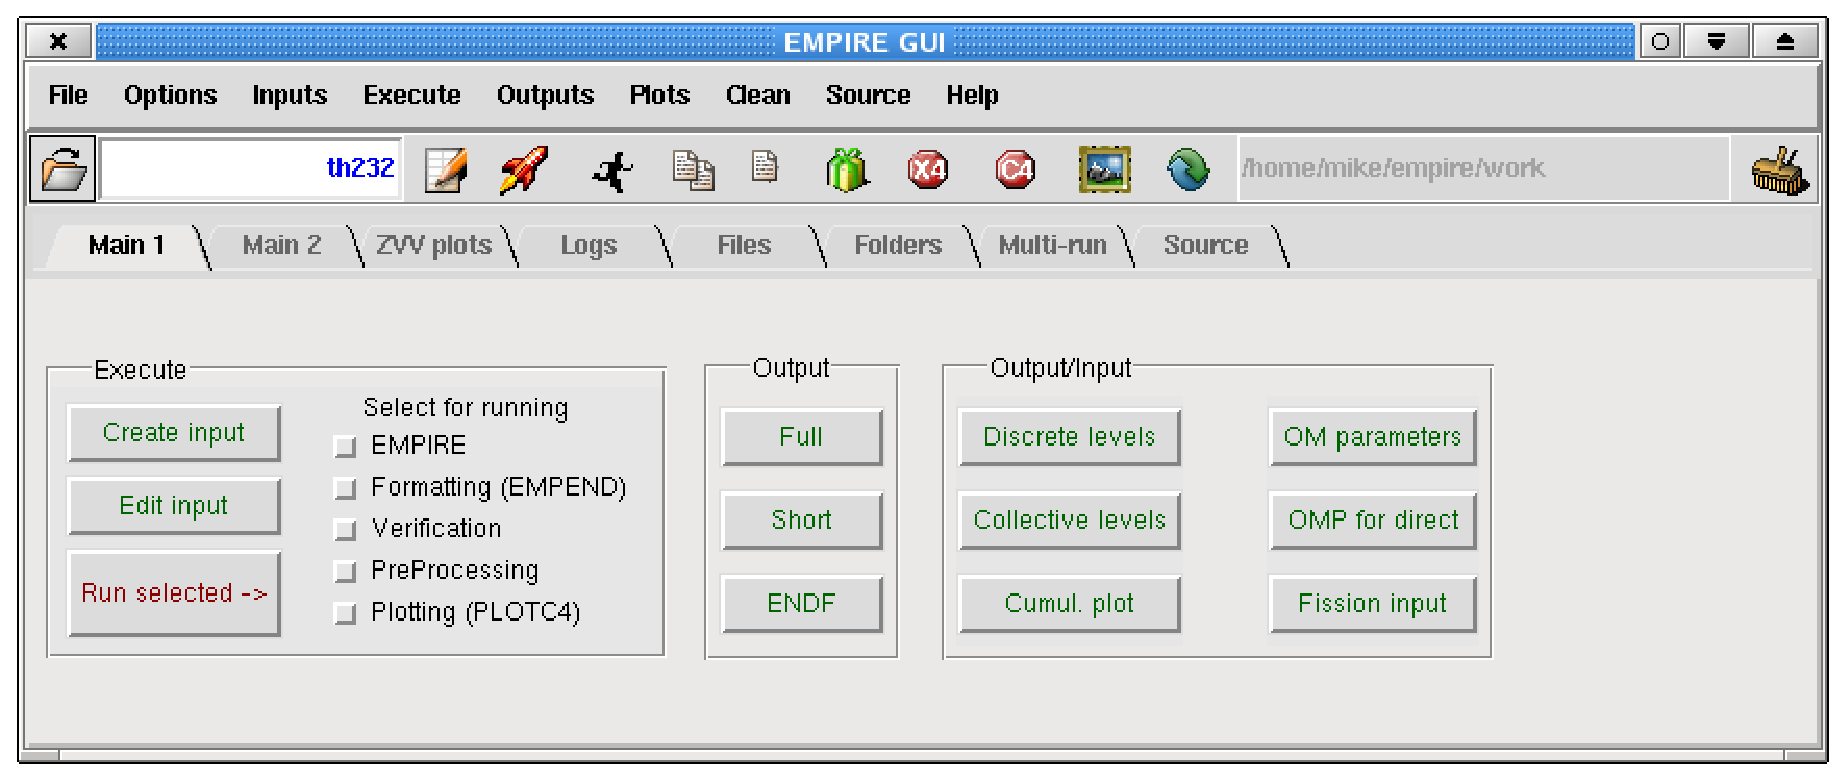
\includegraphics[width=0.75\paperwidth]{figs/GUI-main1}
\caption{\label{cap:EMPIRE-GUI-Main1}EMPIRE GUI - Main1 panel}
\end{centering}
\end{figure}


We start discussion of the GUI with a few features that apply across
the entire interface:

\begin{itemize}
\item Action of many buttons is simply calling an appropriate script with
a project name as an argument. 
\item Double-click on the file in the list will generally open it with the
default application (i.e., text files will be open with the selected
editor, PostScript files with the selected viewer, and {*}.zvd files
will be displayed using ZVView). Within lists typical mouse selection
modes are usually available (although the first file only will be
open for editting): 

\begin{itemize}
\item a single-click selects the file,
\item continuous selection by dragging mouse with the left button pressed, 
\item continuous selection by clicking left mouse button while holding shift
key pressed at the end of the region, 
\item arbitrary multiple selection by clicking left mouse button while holding
'Ctrl' key pressed. 
\end{itemize}
\item Whenever Tcl/Tk allows a `balloon-help' is showed when cursor remains
above the button or icon for a short period of time. This help is
hoped to be sufficient to operate the interface without additional
instructions. Note that if cursor is moved fast across the interface
the 'balloon-help' which appears on the screen might refer to a button
different from the one to which the cursor actually points. To be
sure that the help is correct keep in mind that help string always
starts exactly below the middle of a button or icon. 
\item Colours on the GUI buttons follow 'traffic light scheme' - green means
that pressing button at any time will not make any damage, red warns
that some data or files that have been obtained before or manually
edited might be lost (overwritten). Generally, all buttons involving
editor calls are green while button involving execution of codes or
deleting files are red. Similar distinction is introduced between
the files - red is used for those which are likely to have been manually
edited and green or orange for those which are easy to recreate by
rerunning the code .
\end{itemize}
Due to a large number of operations and extended lists the new GUI
is organized in a form of a notebook with several panels. Generally,
there are several equivalent ways of performing the same operation
and the user my choose the one which suits him best. All basic functions,
such as running the code and viewing the results can be achieved from
the pull-down menus and icon-denoted buttons below the menu bar.
On the other hand, more advanced features such as plotting and file
management can only be accessed from the various panels.

All operations (except multiple run) begin with the selection of the project
name that will be used as a root of the input file name (say 56Fe).
Existing project can be selected by clicking on the 'open folder'
icon to the left of the GUI. The following icons (from left to right)
allow to (i) edit input, (ii) launch full chain of calculations, (iii)
run EMPIRE only, (iv) view long EMPIRE output, (v) view short EMPIRE
output, (vi) view ENDF-6 formatted file, (vii) view EXFOR data, (viii)
view EXFOR data in computational format, (ix) view PLTC4 plots, (x)
refresh list of files, (xi) change working directory, and (xii) remove
all files related to the project except input. More operations are
possible from individual GUI panels.

\vspace{2mm}
\textbf{Main1 panel} - (Fig. \ref{cap:EMPIRE-GUI-Main1}) provides
for essential control of calculations. It allows to create a new input
file (clicking on the {}``Create'' button copies the standard input
file \emph{skel.inp} to \emph{56Fe.inp} and opens it for editing),
executing selected parts of the system (physics calculations, formatting,
verification, preprocessing and plotting). One should keep in mind,
that format verification and preprocessing can only be performed if
EMPIRE calculations and ENDF-6 formatting were carried out before,
and plotting is only possible starting from the preprocessed file.
Main1 panel gives also access to output and output/input files produced
by EMPIRE in the first run. 

\vspace{2mm}
\textbf{Main2 panel} - (Fig. \ref{cap:EMPIRE-GUI-Main2}) provides
additional four features for which there was not enough room on the
Main1 panel. %
\begin{figure}[top]
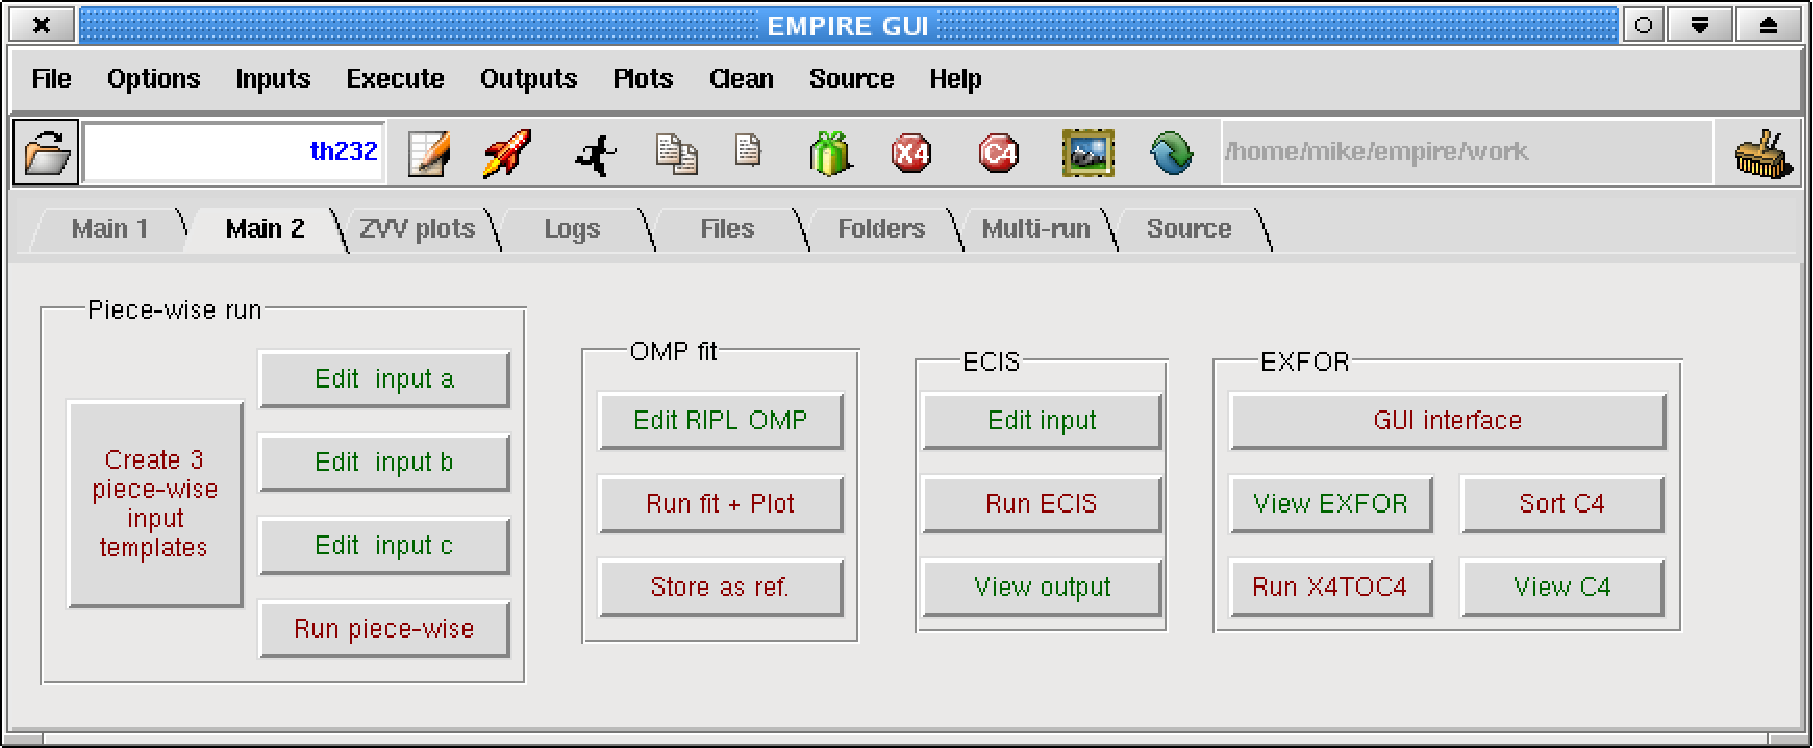
\includegraphics[width=0.75\paperwidth]{figs/GUI-main2}

\caption{\label{cap:EMPIRE-GUI-Main2}EMPIRE GUI - Main2 panel}

\end{figure}


\begin{itemize}
\item 'OMP fit' provides for manual fitting of the optical potential parameters. The three buttons in the frame allow to: (i) open the incident channel optical potential and edit it's content, (ii) run calculations and produce comparison plots of newly calculated cross sections with the reference ones (by default, the first calculation become the first reference), (iii) establish currently modified potential as the new reference potential if it is better than those tried before.

\item EXFOR section will provide access to the Web based EXFOR retrieval that is available
from the IAEA and NNDC web sites. Under normal circumstances this retrieval
is not necessary as experimental data in the C4 format are extracted internally by EMPIRE during the
first run. However, user may choose to use Web retrieval interface
in order to exercise direct control on the retrieved data and take advantage of very powerful features
available through the on-line retrival. These include, automatize application of corrections and generation of covariances for the experimental data if very basic information on the uncertainties is available in the EXFOR file. Last but not least, Web retrieval guarantees access to the most up to date version of EXFOR. When the
EXFOR interface is closed the resulting file with experimental data
is automatically renamed to conform to the current project. It is
up to the user to ensure that the data retrieved are actually relevant
to the calculations. If data are retrieved in the original EXFOR format they have to be converted
into the computational format ('Run X4TOC4' button) and sorted ('Sort
C4' button). The same sequence of buttons should also be used if users
decides to modify the existing \emph{{*}.exf} file (e.g., by removing
or adding certain entries). The recommended option is to download from the Web site the C4 version of the data. This option offers the advantage of using the most up to date and most complete dictionary when translating with the X4TOC4 code, which guarantees the highest  conversion rate and reliability of the conversion of the EXFOR reaction string to the ENDF-6 format specification (MF/MT).  

\item ECIS section allows to view the most recent input and output of ECIS06
code (note that these files are overwritten in each calculation for
each incident energy)
\end{itemize}
~

\textbf{}%
\begin{figure}[top]
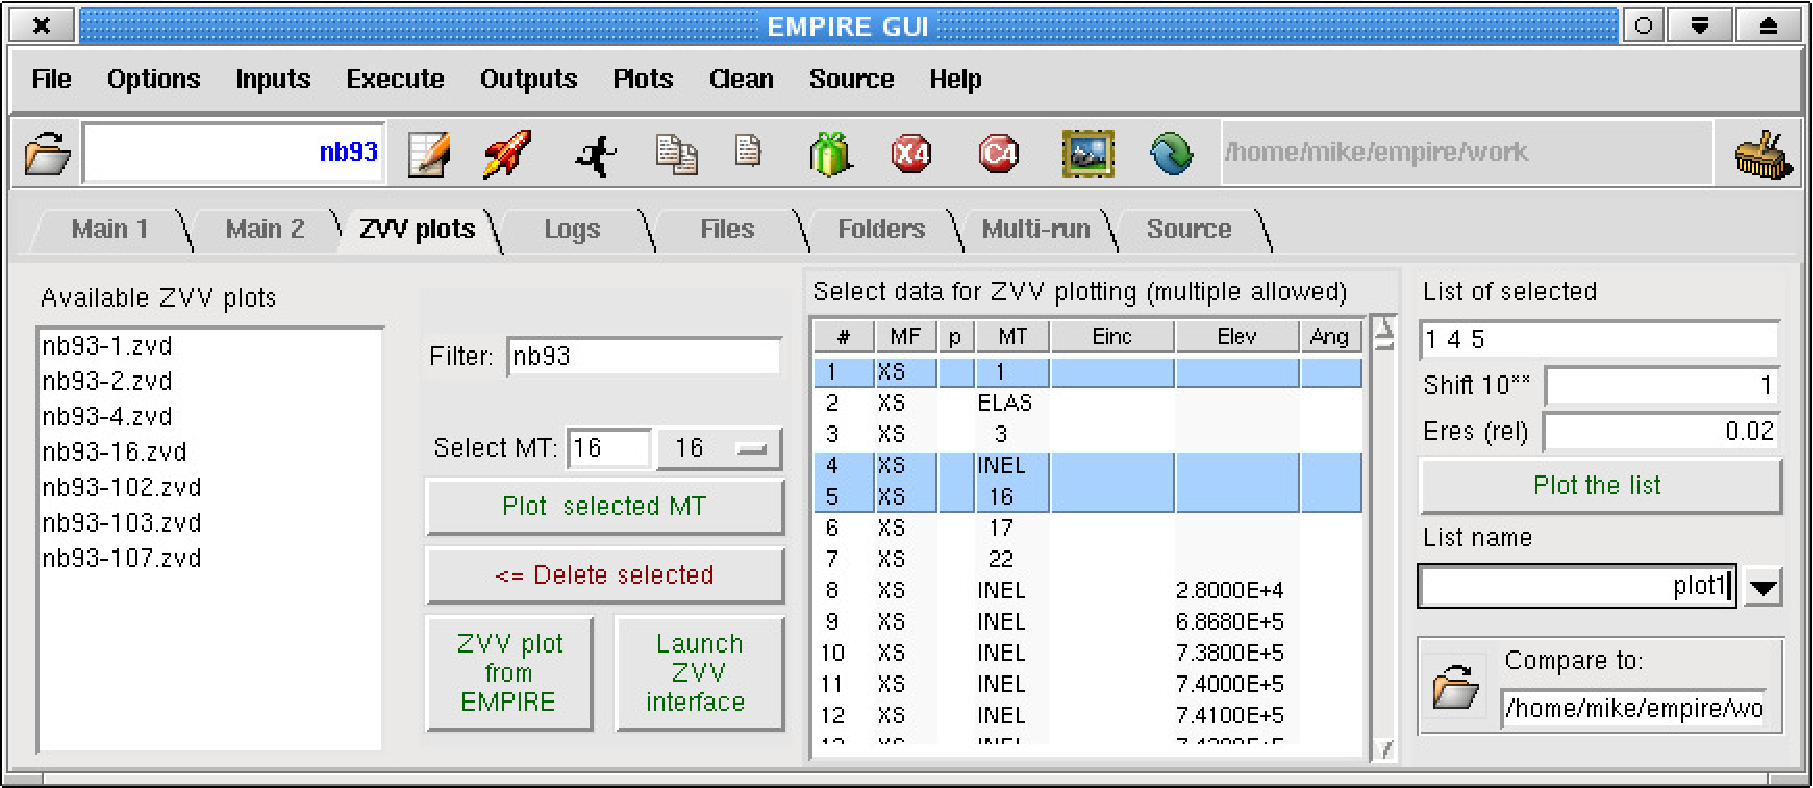
\includegraphics[width=0.75\paperwidth]{figs/GUI-ZVV}

\caption{\label{cap:EMPIRE-GUI-ZVV}EMPIRE GUI - ZVView plots panel}

\end{figure}
\textbf{ZVV plots panel} (Fig. \ref{cap:EMPIRE-GUI-ZVV}) provides
for a powerful interface to the ZVView plotting package. The window
to the left lists all ZVView plots (\emph{{*}.zvd} files) that have
been previously created. User can display them by double-clicking on
any of them. Selecting several plots and double-clicking on the last
one will combine all the selected curves into a single plot. Note
that 'Filter' field allows to restrict displayed files to those containing
filter string in the name (by default Filter is set to the project
name). There are 4 possibilities of creating ZVView files:

\begin{itemize}
\item Selecting MT number and hitting 'Plot selected MT' (note that any
valid ENDF-6 MT number can be typed into the field in addition to
those which can be selected from the predefined list). The MT number
is included in the plot filename for identification (e.g., \emph{56Fe-102.zvd}
for capture). This method allows to plot only excitation functions
(cross sections) for the current calculations (ENDF-6 formatted file
must exist).
\item Hitting 'Launch ZVV Interface' will start more powerful GUI that
allows to create the same type of plots as before but including up
to 3 additional ENDF-6 formatted files for comparison. 
\item 'ZVV plots from EMPIRE' is a bit cumbersome way of creating a cross
section ZVView plot by selecting unique string identifying output
line containing the cross section of interest, pasting it into the
other window and filling additional information (next line, title,
etc.) as requested. The advantage of this method is that the ENDF-6
formatted file is not required and any cross section (number followed
my 'mb') in the long output (\emph{{*}.lst}) can be plotted. This
includes quantities that can not be plotted with the previous methods
since not stored in the ENDF-6 formatted file (such as cross sections
for the population of discrete levels in any nucleus or intensities
of $\gamma$-rays).
\item Selecting plots from the window to the right of the GUI (list created
by PLOTC4 or \emph{pltlst} script). This is the only possibility of
plotting angular distributions, and energy spectra with the ZVView
package. For the relevant line being included in the list there must
be a match between experimental data and calculations (i.e., plots
are only possible if adequate experimental data are available). Multiple
selection can be plotted and each of such selections can be stored
by specifying its name in the 'List name' field. When multiple selection
is plotted the individual curves are offset from each other by a number
of decades specified in the 'Shift 10{*}{*}' field. It implies that
the \emph{y}-scale be logarithmic unless shift is set to 0. 'Eres
(rel)' is the experimental relative energy resolution used to spread
discrete lines (e.g., elastic) and to smooth continuum in the plotted
energy spectra. The 'Compare to' field allows to select another ENDF-6
formatted file to be included in the plots. Note that in order to
obtain correct plots the additional file should be preprocessed in
a way analogous to the original EMPIRE file (resonances
will not be plotted unless the cross sections are reconstructed
from the resonance parameters and double-differential data will not
be plotted unless converted into the right format).
\end{itemize}
~
\begin{figure}[top]
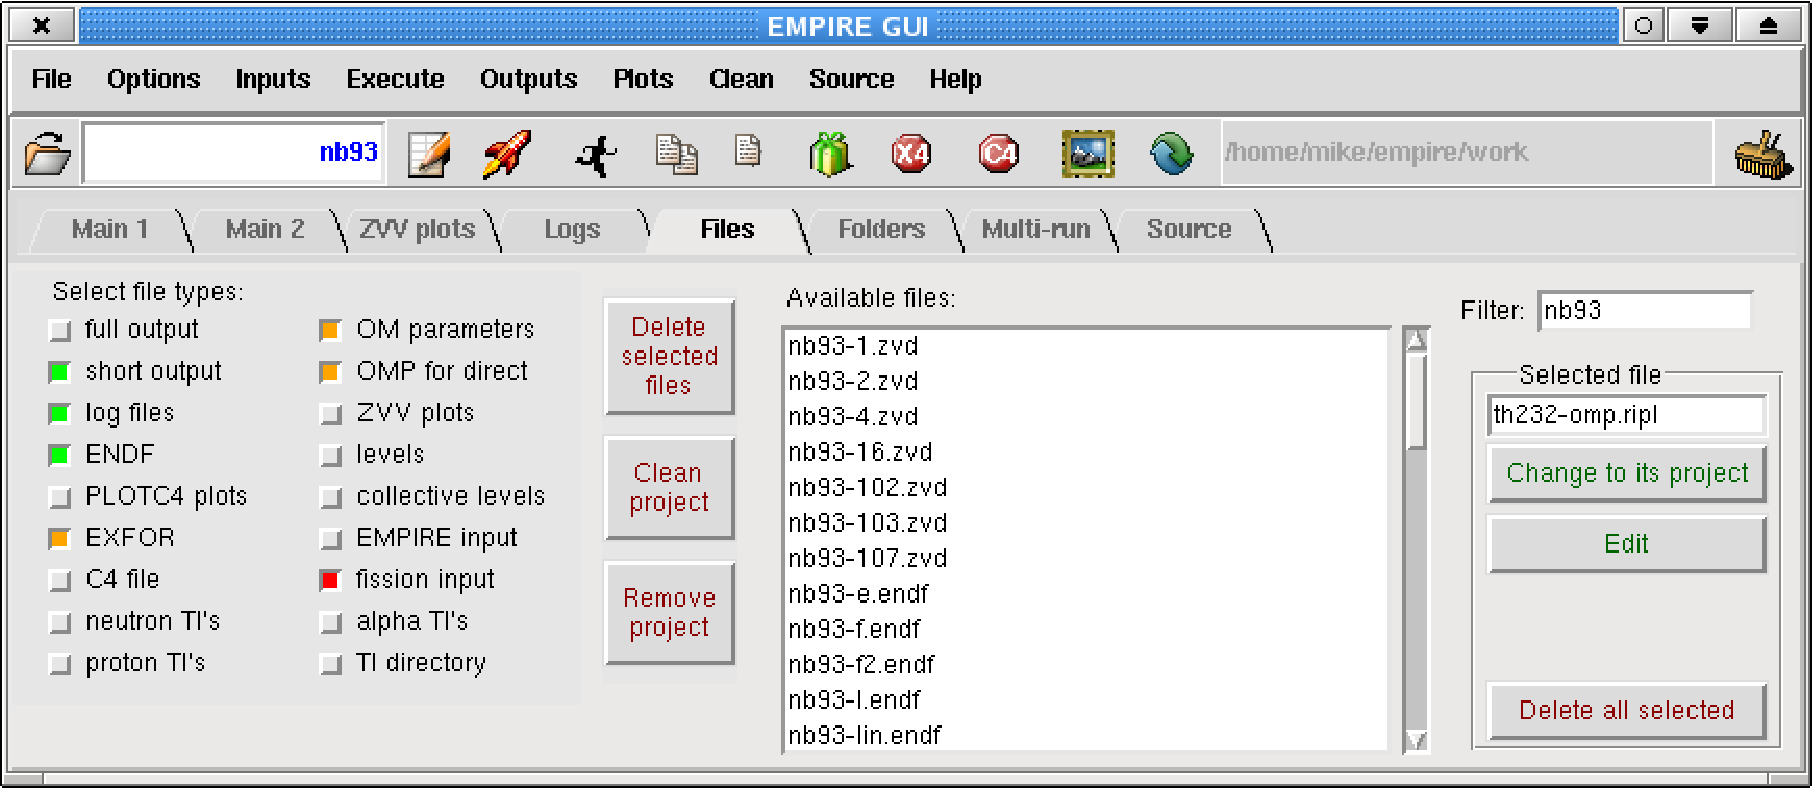
\includegraphics[width=0.75\paperwidth]{figs/GUI-Files}

\caption{\label{cap:EMPIRE-GUI-Files}EMPIRE GUI - Files panel}

\end{figure}


\vspace{2mm}
\textbf{Files panel} (Fig. \ref{cap:EMPIRE-GUI-Files}) offers file
management functions tailored to facilitate operation of the EMPIRE
code. Large number of files produced in a single EMPIRE run might
result in a very crowded working directory if the latter contains
several projects. Files panel is designed to facilitate access to
files belonging to a current project by setting default value of the
filter to the root-name of the project. User can modify filter value
to restrict further list of the files (e.g., filter set to \emph{56Fe{*}endf}
will show only files with extension {*}.\emph{endf} belonging to the
\emph{56Fe} project) or relax it to display more files (e.g., filter
set to \emph{inp} will show input files for all projects). We note
that, selecting a file with a name consisting only of the root-name
and extension (e.g., \emph{56Fe.exf} but not \emph{56Fe-log.psyche)}
and hitting 'Change to its project' button is a convenient way of
redirecting GUI toward another project. The left part of the panel
provides for a convenient removal of the selected types of files belonging
to the current project. In addition, individual files can be removed
by clicking on the 'Delete all selected' button. A double-click on
any of the listed files will open it with an appropriate application.


\vspace{2mm} 
\textbf{Archive panel} - (Fig. )
This panel is intended for storing milestone results of the project in the local or remote Svn repository for the archival purpose that allows to  track development of the project over time and restore certain calculations if needed. In particular, one can easily produce comparison plots  between any two stored versions or between the current and any of the stored versions. 

\vspace{2mm}
\textbf{Folders panel} - (Fig. )
The folders panel is a sort of simple file manger that allows edit and delete files in the subdirectories of empire/.  EMPIRE specific feature of which differs Folders panel from other and arguably more versatile file mangers is the capability of creating the new folder and moving there all the files related to a given
 EMPIRE project (creating an archival copy) leaving in the original directory only those files that are need to continue calculations. Similarly to the File panel  the Folders panel contains Filter that is very useful to narrow down displayed files, e.g., only \emph{{*}-*.zvd} files of the given project.  
  

\vspace{2mm}
\textbf{Multi-run panel} - (Fig. )
'Multi-run' panel allows to perform massive calculations for many nuclei with a few  mouse clicks. The left hand side window allow to load the full set of stable isotopes ('Load all' button is not yet functional). Then one can select an arbitrary number of the isotopes to create a list of targets (the list can be given a name and stored for future use). Unstable isotopes can be added to the list from the input field under the second window from the left. The output files to be kept after calculations must be selected using 'Keep only' radio-buttons. At least one 'green light' is needed to run calculations. This is enforced  to protect user against running hours of calculations only to find out that all the files were deleted right after each calculation was completed. All calculations are performed in the same directory, selected in the input field in the upper-right corner of the GUI. If the input files do not exist they are created form the default skel.inp file by replacing 'xxx'  in the second line of the input by actual mass and atomic numbers. User has a full control of the input by adjusting skel.inp accordingly. Once the actual input files are created they are being reused in the subsequent run. In between the runs, user may introduce arbitrary modifications to the input files.  EMPIRE automatically generates 'root' names combining 'za' prefix with a typical ENDF Z*1000+A.  

\vspace{2mm}
\textbf{Source panel} - (Fig. )
Source panel allow easy access to the FORTRAN modules in the empire/source directory.  Each module can be edited, dimensions can be changed and empire executable can be recompiled. There is also a button for building the whole EMPIRE package. 


%
%\section{Fitting Optical Model Parameters}
%
%When the FITOMP option is selected in the input, EMPIRE will perform
%automatic fitting of parameters in the direct optical model parameter
%file, OMPAR.DIR ({*}-omp.dir), and of deformation parameters in the
%file containing the collective target levels, TARGET\_COLL.DAT ({*}-lev.col).
%The fitting procedure also uses the experimental data file in C4 format,
%C4.dat ({*}.c4). To ensure the existence of these files, EMPIRE should
%be executed at least once before fitting begins and should be executed
%with the DIRECT option selected and an incident channel optical potential
%(initially) defined using the DIRPOT option, both in the initial run
%and during fitting. At the moment, the FITOMP option only works for
%neutron or proton scattering. 
%
%All data relevant to an optical model fit - total, elastic and collective
%inelastic cross sections and elastic and collective inelastic angular
%distributions - within the requested energy range are selected from
%the C4.dat file and included in the $\chi^{2}$ to be minimized. The
%data points in the $\chi^{2}$are weighted in the standard manner
%using the experimental uncertainties given in the C4.dat file. Natural
%element data can be inserted in the C4.dat file and used in the fit.
%In the case of neutron scattering, the file \emph{empire/RIPL/resonances/resonances0.dat}
%is also searched for an s-wave strength function, which is included
%in the experimental data set when found. 
%
%The lower limit of the energy range for calculations used in a fit
%is initially taken to be 1 keV while the upper limit is taken to be
%30 MeV, unless modified using the FITEMX option in the input. All
%relevant experimental data within this range in the C4.dat are included
%in the $\chi^{2}$. The incident energies given in the input file
%define the grid of energies used for calculations, unless the FITGRD
%option is used. When the input file energies are used, the data points
%outside of the energy interval they define are not taken into account.
%That is, the fitting procedure will interpolate calculations but will
%not extrapolate them. When the FITGRD option is used, the energy interval
%is extended to include all data points in the initial energy range.
%In both cases, the grid of incident energies is compared with those
%of the experimental data and superfluous values are eliminated to
%speed up the calculation. 
%
%The parameters to be adjusted are specified by using the FITabc or
%FITDEF options, described in more detail below. The RIPL parametrization
%described in Refs.~\cite{RIPL2,RIPL3} is used to identify the optical
%model parameters, any of which may be adjusted. The adjustable deformations
%are simply those of the collective level file. Quadrupole and hexadecapole
%deformations are permitted for nuclei identified as rotational, while
%quadrupole and octapole deformations are permitted for those identified
%as vibrational. The FITabc and FITDEF options typically identify the
%desired parameter and furnish a shift in its initial value and the
%maximum variation allowed during the fit with respect to its (shifted)
%initial value. If no parameter adjustment is requested or all adjustable
%(possibly shifted) parameters have a maximum allowed variation of
%zero, the $\chi^{2}$ is calculated but no fitting is performed. At
%most 20 parameters may be shifted and/or adjusted simultaneously.
%
%At present, the optical model fitting is performed using a simple
%numerical gradient search to minimize the $\chi^{2}$. The adjusted
%parameters are stored in the modified OMPAR.DIR ({*}-omp.dir) and
%TARGET\_COLL.DAT ({*}-lev.col) files. Information on the fit is written
%in the FIT.OUT ({*}-ompfit.lst) file. When a fit is complete, EMPIRE
%is run one last time with all options and energies given in the input
%file, excepting the fit ones. 
%



%================================================================
\section{Input/Output files}
%================================================================

\subsection{\label{sec: input}{*}.inp (INPUT.DAT; main input)}

EMPIRE is set up to read as much data as possible from the RIPL input directory
\emph{empire/RIPL/} \cite{RIPL} and the local input parameter library 
(\emph{empire/data}). The user has to supply only those input
parameters that the code can not know. These are the incident energy,
the projectile, the target and the number of emitted particles to be followed.
The current version can treat multiple emissions of the following ejectiles:
neutrons, protons, $\alpha$, deuterons, tritons, helions($^3$He) and light ions. 

With the default library of input parameters it is possible to execute
a 'first-shot' calculation with minimal effort. In the second step,
the user may wish to regain control over the input in order to make
appropriate adjustments to the parameters. This can be done in a selective
way in the optional part of the EMPIRE input, or directly in local project files
produced by EMPIRE during its first run. 

It should be noted that there is a difference in the way EMPIRE accesses
general input library in the first and subsequent runs of a given
project. In the first run the code extracts relevant data from the
input parameter library and creates local project files with discrete levels ({*}.\emph{lev}),
collective levels (\emph{{*}-lev.col}), optical model parameters (\emph{{*}-omp.ripl},
and \emph{{*}-omp.dir}), fission parameters \emph{{*}-inp.fis} and relevant 
EXFOR data ({*}.\emph{exf} and {*}.\emph{c4}) files. Once these files 
exist the code uses them instead of the files contained in the general input library.
This has two advantages: (i) time is spared because the case specific files are
smaller and can be read fast, (ii) the user may edit case specific files {*}.\emph{lev,
{*}-omp}.{*}, \emph{{*}-inp.fis)}, and {*}.\emph{c4} files and modify them 
without affecting files in the general input library. Editing the \emph{{*}-omp.{*}}
files is a convenient method of adjusting some of the optical model
parameters without the necessity of typing the whole set from scratch.
Editing the fission parameter \emph{{*}-inp.fis} file is a convenient method
of adjusting fission parameters; editing the collective level file allows for a
selection of additional coupled levels, discrete levels embedded in the continuum, etc. 

Input data are taken from different sources in the following decreasing priority
(i.e. those listed above overwrite those listed below):

\begin{enumerate}
\item case specific files (\emph{{*}.lev, {*}-lev.col, {*}-omp}.{*}, \emph{{*}-inp.fis})
\item input file ({*}.\emph{inp})
\item general input parameter library including both the local and RIPL libraries
\end{enumerate}
Note, that all the case specific files, except (\emph{{*}.inp}), are created by the
code during the first run, and therefore the user has to create only
the (\emph{{*}.inp}) file described below.

\subsubsection*{Mandatory input }

Input to EMPIRE consists of two parts. The first is mandatory and
contains basic data necessary to specify the case, and the structure
is illustrated by the following example: 
\begin{verbatim}
14.8                       ;INCIDENT ENERGY (IN LAB)
56      26                 ;TARGET A , Z
 1     0                   ;PROJECTILE A, Z
3                          ;NUMBER OF NEUTRONS TO BE EMITTED
1                          ;NUMBER OF PROTONS TO BE EMITTED
1                          ;NUMBER OF ALPHAS TO BE EMITTED
1                          ;NUMBER OF DEUTERONS TO BE EMITTED
1                          ;NUMBER OF TRITONS TO BE EMITTED
1                          ;NUMBER OF HELIONS (3He=h) TO BE EMITTED
0      0.     0.           ;NUMBER OF L.I. TO BE EMITTED, AND ITS A AND Z
\end{verbatim}
The first line specifies the incident energy in the laboratory system
(in MeV). The second and third are used to specify the mass and
atomic numbers of a target and a projectile respectively. The next
seven lines define the number of emissions to be followed for each
ejectile. In the above example, all reactions up to 
(n,3np$\alpha$dth) will be calculated. The code automatically sums 
over all possible decay sequences to reach the given residual nucleus. 
Accordingly, each reaction includes all possible permutations of ejectiles
(e.g. $\sigma_{(n,npd)}=\sigma_{(n,2n2p)}+\sigma_{(n,dd)}+\sigma_{(n,nh)}+
\sigma_{(n,\alpha)}+\sigma_{(n,pt)}$. The last line of the mandatory input 
provides for the inclusion of the emission of one type of heavy or light ion.
This option is provided for backward compatibility (and future development).
The current EMPIRE version does not allow emission of ions heavier than the 
$\alpha$-particle (all lighter ions are accounted for explicitly). 
If such need arises, please contact the authors.

%
%The library of optical model parameters allows for $^{6}$Li,  $^{7}$Li, and $^{7}$Be ejectiles. 
%
%If the incident projectile is a heavy ion, then it is recommended that the last line
%contains the same incident heavy ion, therefore providing the possibility for the 
%calculation of the elastic channel. The reaction cross sections for heavy ion reactions
%can be calculated by using an approximated optical model treatment (e.g., CCFUS), or can be
%read in the optional input (see CSREAD parameter below).  Use of the light ion ejectile option 
%requires the code to be compiled with NDEJC set to 7 in the file \emph{dimension.h}. 
%If the last line of the mandatory input consists of three zeros (as in the example) 
%the light/heavy ion emission channel is closed regardless of the NDEJC value
%used in the compilation.
%If the last line of the mandatory input consists of three zeros (as in the example) 
%the light/heavy ion emission channel is closed regardless of the NDEJC value
%used in the compilation.

The mandatory part of the input is in a free format, while the comments
following the semicolon only serve to facilitate input preparation
and are ignored by the code. 

\subsubsection*{Optional input}

The mandatory input is followed by optional input, which allows modifications
to the default model parameters. Optional input consists of an arbitrary
number of records, entered in any order and closed with the GO record,
which indicates the end of the input. In the simplest case (all defaults),
only the GO record must be entered. Each optional record starts with an alphanumeric
keyword {\bf NAME}. If the first character of the line (i.e. {\bf NAME(1:1)}) is {\bf *}, {\bf \#}
or {\bf !}, then this line contains comments and is ignored by the code.
If the first character of the line {\bf NAME(1:1)} is {\bf @}, 
then this line contains a title, which will be printed in EMPIRE outputs; obviously
the title is not used in any calculations. Multiple titles are allowed.
Users are strongly encouraged to use titles and comments in EMPIRE inputs; that will be a 
significant step toward a better documentation of our theoretical calculations 
and evaluations.\\

The optional-input keyword {\bf NAME} is followed by the value VAL and four positional
parameters I1, I2, I3, I4. The keyword indicates a physical quantity, such as the
binding energy or level density parameter, or a scaling parameter (e.g. TOTRED) . 
VAL takes numerical value  of the  quantity or scaling parameter).  \\
The  positional parameters are typically  used to  specify to which nucleus the quantity 
should be applied (generally  if these are omitted  the value is applied to all
nuclei in the given calculation). Positional parameters may be also used to 
indicate the estimated uncertainty of the quantity defined by the input keyword 
(except optical model parameters for which the uncertainty is defined by VAL). 
Each record must be in the FORTRAN fixed-length format:
\begin{quote}
FORMAT (A6,G10.5,4I5) {\bf NAME},VAL,I1,I2,I3,I4
\end{quote}
Fixed format allows to avoid typing zeros if no input is needed for some 
positional parameters, but attention should be paid by user to keep 
numbers in the right position.

The GO record indicates end of the optional input and starts calculations. 
It may be followed by an unlimited list of incident energies
(one per record) terminated with a record containing a negative value.
Anything below this line will be ignored by the code. 

% If no line with 
% negative value is found, then the code will terminate at the end of file (EOF). 

A complete list of model parameters and options that can be
controlled through the optional input entries is given in the Appendix \ref{InputList}. 


%================================================================
\subsection{{*}-inp.fis (FISSION.INP)}
%================================================================
\label{fis-inp}

This file is created and used only if FISSHI=0. It collects all incident energy independent input parameters
related to fission of the nuclei involved in reaction for which the fissility condition is fulfilled.  
It follows general EMPIRE philosophy of input/output files: it is created by the code if missing  
and it is read by the code if it exists.
All numerical values in this file representing default fission parameters may be changed except those for 
which it is said explicitly otherwise.

\noindent The  \emph{{*}-inp.fis} file must be deleted manually if one of the following changes has been done in main input:
\begin{itemize}
\item[ ] FISBAR = 3 $\leftrightarrow$ FISBAR $<$3
\item[ ] FISMOD = 0 $\leftrightarrow$ FISMOD $>$0
\end{itemize}
If FISOPT = 0 $\rightarrow$ FISOPT $>$ 0 one has to make sure that the number of transition states at each
extremum is the same.

\noindent The \emph{{*}-inp.fis} file is divided into sections corresponding to each fissioning
nucleus. Each section starts with the key-word ``Isotope''. Therefore in the following examples
we will have as reference the line containing ``Isotope'' denoted L=1.

\paragraph {Example 1}
Fission input created if FISSHI=0; FISOPT=0,1,2,3; FISBAR$<$3, FISDEN=0,2; FISDIS=0,1; FISMOD=0

\begin{itemize}
\item[- ] {L=6} - 
 number of parabolas $N_{parab}$(used to describe the entire barrier) and  number of wells $N_w$
(the number of minima excluding the one corresponding to equilibrium deformation);  they cannot be changed.
%
\item[- ]{L=9} -
parameters of the fundamental barrier in the following order:
pairs of height- width ($E_{f_h(w)}, \hbar\omega_h(w)$) for each hump (maximum) followed by similar pairs for 
the wells, all expressed in MeV;
these  parameters entering Eq. \ref{vfund0} have initial values depending on FISBAR. 
%
\item[- ]{L=12} - 
inertial parameters ${\hbar^{2}}/{2\Im_{h(w)}}$ used in Eq.~\ref{tsrot} to build rotational levels in MeV.
%
\item[- ]{L=15} -
quadrupole deformations corresponding to the extrema of the fission barrier. The values printed
correspond to the initial barrier parameters. If barrier parameters have been modified, EMPIRE calculates 
and uses the new deformations which are printed in \emph{*-fiss.out} but not in \emph{*-inp.fis}. Therefore
their change would have no impact.
%
\item[- ]{L=20+$w;~ (w=1,N_w$)}     -
parameters used in the energy dependence of the strength of the imaginary potential corresponding to each well
(Eq.~\ref{wimag}). There are two differences compared to the older version of the code: (i) the energy 
dependence was changed, therefore the values of $W_i (i=1,3)$ are changed accordingly, and (ii) there is a set 
of parameters for each well (instead a single set as it was before), meaning that to make them compatible 
with the present version of the code, the old files containing triple-humped barrier have to be changed
by copying L=21 in L=22 also.

%
\item[- ]{L=25+$N_w$} -
number of discrete states for the first hump $N_{dis}(h_1)$. It is writen and read as 'I2'  format starting after 
``='' sign and has the maximum value equal to 30.  For FISOPT$>$0 The number of discrete states and their order 
($K\pi$) must be the same. For FISOPT=0, the discrete states number might differ from one hump to another.
However their values have to be equal to the number of lines below, associated to each discrete state.
%
\item[- ]{L=26+$N_w+k;~ (k=1,~N_{dis,h}$)} -
spin projection on the symmetry axes, parity and excitation energy with respect to the top of the hump
 $K,\pi,\epsilon_h$ (entering  Eq.~\ref{tsrot}) plus the width $\hbar\omega_h$ for all 
discrete transition states (rotational band-heads) at hump $h$.
This sequence of lines plus the one above are repeated for each extremum: first for the humps and next for the
wells. 
All the numbers on these lines can be changed but keeping in mind that for FISOPT$>$0 the number of discrete
states and the order of $K\pi$ must be the same for all extrema.
%
\item[- ]{L=29+$N_w+[N_{dis,h}+2]*N_{parab}+h;~(h=1,N_h)$} - 
data used for FISDEN=0: 
hump index, degree of asymmetry of the nuclear shape at saddle $B_{sym,h}$, shell-correction $\delta W_{f_h}$, 
energy shift $\delta_h$ in the efective excitation energy, $\gamma_{f,h}$ , 
the ratio $\tilde a_{f,h}/\tilde a$ of the asymptotic values for saddle and equilibrium deformations,
the lower limit of transition state continuum spectrum $E_{c,h}$, parameters defining vibrational damping
$T_{1/2,h}, DT_h$ and the global scaling factor $N_h$.


The degree of asymmetry has the following significance
\begin{equation}
B_{sym,h}=\left\{
\begin{array}{lll}
1 & {\rm axial,~ mirror~ symmetry}& h=1,\quad N<144) \\%({\rm ~inner~barrier} N$<$144) \\
2 & {\rm axial~ asymmetry,~ mirror~ symmetry}& h=1,\quad N\geq 144) \\%({\rm ~inner~barrier} N\geq 144) \\
3 & {\rm axial~ symmetry,~ mirror ~asymmetry}& h=2,(3)\\% ({\rm ~outer barrier(s)})\\
\end{array}
\right..
\label{b_sym}
\end{equation}
and selects the values of $f_{sym}$ (Eq.~\ref{f_sym}) and $d_{sym}$ (Eq.~\ref{d_sym}).

\item[- ] {L=34+$N_{parab}+[N_{dis,h}+2]*N_{parab}+h;~(h=1,N_h)$} - data used for FISDEN=2: 
the degree of asymmetry of the nuclear shape at saddle $B_{sym,h}$ and the normalization parameters
$\delta_h$, $\alpha_h$ and $N_h$ from Eq.~\ref{HFB-fis}.

\item[- ] {L=38+$N_{parab}+[N_{dis,h}+2]*N_{parab}+N_h+w;~(w=1,N_w)$} - weights $p_w$ entering Eq.~\ref{tfsurr};
if nonzero, direct transmission in continuum is added to the direct transmission coefficient. 
\end{itemize}

\noindent Below is a real example of the fission input file corresponding to the cases discussed above. 
{\footnotesize
\begin{verbatim}
Isotope:
----------------------------------------
    Z= 92  A=238
----------------------------------------
  
 Nr.parabolas =3      Nr.wells=1
 
    Va      ha      Vb      hb      Vi      hi  (in Mev) 
   6.300   0.800   5.700   0.500   1.400   1.000
  
  h2/2J(A)  h2/2J(B)  h2/2J(I)  (in MeV)
   0.0050   0.0025   0.0035
  
  Beta2(A)  Beta2(B)  Beta2(I)
   0.4099   0.9337   0.6285
   
 ======================================================================
  Parameters of the imaginary potential used only if FISOPT>0
 ======================================================================
       W0         W1         W2
     1.0000     0.1000     0.1000
 
 ======================================================================
  Discrete transitional states
 ======================================================================
   Number of discrete states at barrier 1 = 2
 Jdis  Pidis   Edis    homega
 0.0   -1     0.700    0.800
 1.0   -1     0.400    0.800
   Number of discrete states at barrier 2 = 2
 Jdis  Pidis   Edis    homega
 0.0   -1     0.100    0.500
 1.0   -1     0.500    0.500
   Number of discrete states at barrier 3 = 2
 Jdis  Pidis   Edis    homega
 0.0   -1     0.000    1.000
 1.0   -1     0.000    1.000
 
 ======================================================================
  Quantities used only if FISDEN=0 to calculate LD at saddles
 ======================================================================
              Asym shell-corr delta    gamma atilf/ati   Ecf     VIB1/2   VIBdt    Norm
  Barrier 1    2    2.600    0.307    0.600    1.000    0.000    1.000    0.100    1.000
  Barrier 2    3    0.220    0.307    0.600    1.000    0.000    1.000    0.100    1.000
 
 ======================================================================
   Coefficients used only if FISDEN=3 to adjust HFB LD at saddles 
 ======================================================================
             Asym    Delta    alpha   Norm
 Barrier  1    2    0.000    0.000    1.000
 Barrier  2    3    0.000    0.000    1.000
 
 ======================================================================
   Coefficient(s) used to calculate the direct continuum weight(s) 
 ======================================================================
     Well 1    0.000
 
 ****************************************************
 ****************************************************
\end{verbatim}
}



\paragraph {Example 2}
Fission input created if FISSHI=0; FISOPT=0,1,2,3; FISBAR=3, FISDEN=0,2; FISDIS=0; FISMOD=0

\begin{itemize}
\item[- ] {L=9} - number of points $N_p$ for which the numerical path is defined; cannot be changed.
\item[- ] {L=9+$n;~(n=1,N_p$} - index $n$, fission potential $V(\beta)_n$, quadrupole deformation $\beta_n$.
\item[- ] {L=11+$N_p$} -  number of parabolas $N_{parab}$(used to describe the entire barrier) and  number of wells $N_w$
(the number of minima excluding the one corresponding to equilibrium deformation);  they cannot be changed.
\item[- ] {L=14+$N_p$} - indexes of extrema; they cannot be changed.
\item[- ] {L=16+$N_p$} - normalization factors for the numerical barrier: $n_{b,h};~ (h=1,N_h)$, $n_{\beta}$.
The width scaling $n_{\beta}$ enters Eq.~\ref{w-norm}, and the independent height normalization factors
$n_{b,h}$ enter Eq.~\ref{b-norm2}. If $n_{b,1}$=10, then $n_{b,2}$ represents the global normalization factor
entering Eq.~\ref{b-norm1}.
It should be mentioned that the effect of normalization can be seen in *fis.out, but not in *inp.fis.
\item[- ] Subsequent lines contain the same information as presented in Example 1. 
\end{itemize}
\noindent Below we show an example of the fission input file with numerical fission barriers. 

{\footnotesize
\begin{verbatim}
Isotope:
----------------------------------------
    Z= 92  A=239
----------------------------------------
  
 ======================================================================
  RIPL-3 HFB numerical fission barrier
 ======================================================================
 96
   1     0.000     0.307
   2     0.648     0.336
   3     1.565     0.364
   4     2.597     0.388
   5     3.468     0.413
...
  94     0.475     2.888
  95     0.462     2.889
  96     0.000     2.890
 
 Nr.parabolas =5      Nr.wells=2
  
  Index of extrema
          10          20          36          55          58
  Normalization factors for humps
     0.000     0.000     0.000     1.000
 ======================================================================
    Va      ha      Vb      hb      Vc       hc      Vi      hi      Vo      ho  (in Mev) 
   5.990   0.652   6.542   0.403   3.675   0.086   1.798   0.505   3.317   0.163
  
  h2/2J(A)  h2/2J(B)  h2/2J(C)  h2/2J(I)  h2/2J(O)  (in MeV)
   0.0050   0.0025   0.0017   0.0035   0.0020
  
  Beta2(A)  Beta2(B)  Beta2(C)  Beta2(I)  Beta2(O)          
   0.5480   1.2610   1.8600   0.8810   1.7610
  
 ======================================================================
  Parameters of the imaginary potential used only if FISOPT>0
 ======================================================================
       W0         W1         W2
     1.0000     0.1000     0.1000
     1.0000     0.1000     0.1000
 
 ======================================================================
  Discrete transitional states
 ======================================================================
    Number  of  discrete states at hump 1 = 4
 Kdis  Pidis   Edis    homega
 0.5    1     0.000    0.652
 2.5    1     0.080    0.652
 0.5   -1     0.050    0.652
 1.5   -1     0.010    0.652
    Number  of  discrete states at hump 2 = 4
 Kdis  Pidis   Edis    homega
 0.5    1     0.000    0.403
 2.5    1     0.010    0.403
 0.5   -1     0.010    0.403
 1.5   -1     0.080    0.403
    Number  of  discrete states at hump 3 = 4
 Kdis  Pidis   Edis    homega
 0.5    1     0.000    0.086
 2.5    1     0.000    0.086
 0.5   -1     0.000    0.086
 1.5   -1     0.000    0.086
    Number  of  discrete states in well 4 = 4
 Kdis  Pidis   Edis    homega
 0.5    1     0.000    0.505
 2.5    1     0.000    0.505
 0.5   -1     0.000    0.505
 1.5   -1     0.000    0.505
    Number  of  discrete states in well 5 = 4
 Kdis  Pidis   Edis    homega
 0.5    1     0.000    0.163
 2.5    1     0.000    0.163
 0.5   -1     0.000    0.163
 1.5   -1     0.000    0.163
 
 ======================================================================
  Quantities used only if FISDEN=0 to calculate LD at saddles
 ======================================================================
              Asym shellcorr Ushif    gamm  atilf/atil   Ecf     VIB1/2   VIBdt    Norm
  Barrier 1    2    2.600    0.300    0.600    1.000    0.000    1.000    0.100    1.000
  Barrier 2    3    0.260    0.300    0.600    1.000    0.000    1.000    0.100    1.000
  Barrier 3    3    0.260    0.300    0.600    1.000    0.000    1.000    0.100    1.000
 
 ======================================================================
   Coefficients used only if FISDEN=3 to adjust HFB LD at saddles 
 ======================================================================
             Asym    Delta    alpha   Norm
 Barrier  1    2    0.000    0.000    1.000
 Barrier  2    3    0.000    0.000    1.000
 Barrier  3    3    0.000    0.000    1.000
 
 ======================================================================
   Coefficient(s) used to calculate the direct continuum weight(s) 
 ======================================================================
     Well 1    0.000
     Well 2    0.000
 
 ****************************************************
 ****************************************************
\end{verbatim}
}


\paragraph {Example 3}
Fission input created if FISSHI=0; FISOPT=0; FISBAR$<$3, FISDEN=0; FISDIS=0,1; FISMOD=2

The file structure is the one described in Example 1, therefore will be mentioned only the differences
specific to multimodal fission. In general the parameters for the outer barrier are doubled, if FISMOD=1,
describing (SL) and (S1) or tripled, if FISMOD=2, describing (SL),(S1) and (S2).

\begin{itemize}
\item[- ]{L=9} -
parameters of the fundamental barrier in the following order:
pairs of height- width ($E_{f,1}, \hbar\omega_1$),($E_{f,SL}, \hbar\omega_{SL}$),($E_{f,S1}, \hbar\omega_{S1}$),
($E_{f,S2}, \hbar\omega_{S2}$)  followed by similar pairs for the wells, all expressed in MeV;

\item[- ]{L=28+$N_w+N_{dis}+k;~ (k=1,~N_{dis,2}$)} -
spin projection on the symmetry axes, parity and excitation energy with respect to the top of the outer humps (SL),(S1) and (S2):
$K,\pi$, and pairs height-width ($\epsilon_2$ -  $\hbar\omega_2$) for (SL),(S1) and (S2) and for all 
discrete transition states.

\item[- ]{L=30+$N_w+[N_{dis,h}+2]*N_{parab}+h2;~(h2$}=FISMOD+1 - 
data used for FISDEN=0: 
hump index, mod index, degree of asymmetry of the nuclear shape at saddle $B_{sym,h}$, shell-correction $\delta W_{f_h}$, 
energy shift $\delta_h$ in the efective excitation energy, $\gamma_{f,h}$ , 
the ratio $\tilde a_{f,h}/\tilde a$ of the asymptotic values for saddle and equilibrium deformations,
the lower limit of transition state continuum spectrum $E_{c,h}$, parameters defining vibrational damping
$T_{1/2,h}, DT_h$ and the global scaling factor $N_h$ for (SL),(S1) and (S2). 
\end{itemize}
\noindent Below we report  example of the fission input for the multimodal fission. 

{\footnotesize
\begin{verbatim}
Isotope:
----------------------------------------
    Z= 94  A=243
----------------------------------------
  
 Nr.parabolas =3      Nr.wells=1
 
      Va      ha     Vb(SL)    hb(SL)  Vb(ST1)  hb(ST1)   Vb(ST2)  hb(ST2)   Vi      hi  (in Mev) 
    6.050    0.700    7.450    1.200    5.450    0.700    5.550    0.700    2.000    1.000
  
  h2/2J(A)  h2/2J(B)  h2/2J(I)  (in MeV)
   0.0050   0.0025   0.0035
  
  Beta2(A)  Beta2(B)  Beta2(I)
   0.4438   0.9232   0.6634
   
 ======================================================================
  Parameters of the imaginary potential used only if FISOPT>0
 ======================================================================
       W0         W1         W2
     1.0000     0.1000     0.1000
 
 ======================================================================
  Discrete transitional states
 ======================================================================
    Number  of  discrete states at hump 1 = 4
 Kdis  Pidis   Edis    homega
 0.5    1     0.000    0.700
 2.5    1     0.080    0.700
 0.5   -1     0.050    0.700
 1.5   -1     0.010    0.700
    Number  of  discrete states at hump 2 = 4
 Kdis  Pidis   Edis    homega
 0.5    1     0.000    1.200    0.000    0.700    0.000    0.700
 2.5    1     0.010    1.200    0.010    0.700    0.010    0.700
 0.5   -1     0.010    1.200    0.010    0.700    0.010    0.700
 1.5   -1     0.080    1.200    0.080    0.700    0.080    0.700
    Number  of  discrete states in well 3 = 4
 Kdis  Pidis   Edis    homega
 0.5    1     0.000    1.000
 2.5    1     0.000    1.000
 0.5   -1     0.000    1.000
 1.5   -1     0.000    1.000
 
 ======================================================================
  Quantities used only if FISDEN=0 to calculate LD at saddles
 ======================================================================
              Asym shellcorr Ushif    gamm  atilf/atil   Ecf     VIB1/2   VIBdt    Norm
  Barrier 1    2    2.600    0.300    0.600    1.000    0.000    1.000    0.100    1.000
  Barrier 2  1 0    0.540    0.300    0.600    1.000    0.000    1.000    0.100    1.000
  Barrier 2  2 0    0.540    0.300    0.600    1.000    0.000    1.000    0.100    1.000
  Barrier 2  3 0    0.540    0.300    0.600    1.000    0.000    1.000    0.100    1.000
 
 ======================================================================
   Coefficients used only if FISDEN=3 to adjust HFB LD at saddles 
 ======================================================================
             Asym    Delta    alpha   Norm
 Barrier  1    2    0.000    0.000    1.000
 Barrier  2    3    0.000    0.000    1.000
 
 ======================================================================
   Coefficient(s) used to calculate the direct continuum weight(s) 
 ======================================================================
     Well 1    0.000
 
 ****************************************************
 ****************************************************
\end{verbatim}
}

\subsection*{{*}-inp.sen (SENSITIVITY.INP)}
The sensitivity input instructs EMPIRE which parameters should be 
considered in the sensitivity matrix and  how much are they going to be varied. 
Contrary to other input files in EMPIRE, the sensitivity input is not directly 
linked to the particular case since the reference is made to the compound nucleus 
and the nuclei involved in the decay chain are identified by the number of neutrons and protons which were removed from the compound nucleus rather than specifying their actual number (as in the main input file \emph{{*}.inp}). Therefore, the default input
can be used for any nucleus but care should be taken to use only those parameters 
that are relevant to the models and mechanisms used in the actual calculations and, on the other side, to include all the parameters that are relevant to the calculations. For example,
 it makes no sense to vary fission parameters in the case of  neutron reaction on iron, or modifying MSD parameters if MSD is not being used but it's even worse not to vary fission parameters for the case of uranium. 
 
The sensitivity input is created automatically in the first run by copying 
the default file \emph{skel-inp.sen}. As usual in EMPIRE, user is supposed  to adjust this file by taking into account reaction mechanisms and models used in the main input, available experimental data and scope of the research.

The structure of the file follows the optional input in \emph{{*}.inp} - the same keywords  are used except that 
\begin{itemize}
\item the  first parameter (val) specifies the perturbation, e.g., 0.05 means perturbation of the parameter specified by the keyword by 5\%.
\item the second positional parameter  indicates how many protons  were removed from the compound nucleus
\item the third positional parameter  indicates how many neutrons  were removed from the compound nucleus
\item the fourth positional parameters retains its original meaning (usually it indicates an ejectile)
\end{itemize}
For example, the following line of input \\
\begin{verbatim}
UOMPVV     0.03    00  01   1      ! omp real vol. depth for Z N-1 nucl.
\end{verbatim}
indicates that the real depth of the optical model for the neutron (4$^{th}$ parameter equal 1) on the residue nucleus after emitting one neutron from the  compound nucleus (3$^{rd}$ parameter equal 01) will be perturbed by 3\%. 
%
%The typical sensitivity input is given below.
%\begin{verbatim}
%UOMPVV     0.03    00  01   1      ! omp real vol. depth for Z N-1 nucl.
%\end{verbatim}


\subsection{{*}.lst (LIST.DAT; lengthy output)}

As the main output of EMPIRE, the size of the file depends on the
controls IOUT and NOUT specified in input ({*}.\emph{inp}). In the
extreme case, no output except warnings is produced (note that all
essential results are written to the file \emph{{*}.out,} which is
not affected by IOUT and NOUT). 

The file begins with the code banner and printout of the parameters
specified in the optional input. Lack of a message regarding any given
parameter means that the default value has been used in the calculations.
The next segment of the output specifies the incoming channel and
model parameters such as binding energies, fission barriers, shell
corrections, ground state deformations and list of optical model systematics
used in the calculations. The message is printed to notify the user
on eventual re-normalization of the internal level density\index{level density}
systematics to the experimental results. Re-normalization is performed
only if experimental values of the \emph{a}-parameter for at least
3 nuclei involved in the calculations are found in \emph{empire/data/ldp.dat}
. The introductory part of the output is followed by the results of
calculations for each decaying nucleus. 

In the case of Compound Nucleus all calls to the ORION\index{ORION}
code are listed and the outputs of TRISTAN\index{TRISTAN} and ORION
codes (the latter only if $IOUT > 3$) are printed. Next, the fusion
cross section and associated spin/parity distributions are given.
For each decaying nucleus (including Compound Nucleus) the production
cross section, population of discrete levels, intensities of discrete
$\gamma$-lines and emitted spectra of $\gamma$s, neutrons, protons,
$\alpha$s and eventually light ions are printed. Output for a given
incident energy is completed by inclusive spectra of all $\gamma$s
and particles emitted along the de-excitation chain. This scheme is
repeated for each incident energy apart from the code banner and optional
input printout. The general structure of the output can be summarized
as follows (depending on input options some items might be missing
in an output):

\begin{itemize}
\item code banner
\item optional input
\item matrix of models usage
\item 1$^{st}$ incident energy

\begin{itemize}
\item Compound Nucleus

\begin{itemize}
\item input parameters
\item elastic, reaction and total cross sections 
\item inelastic scattering to collective levels 
\item pre-equilibrium models' results
\item fusion cross section
\item population and decay of discrete levels 
\item residue production cross section
\item fission cross section
\item emission spectra
\end{itemize}
\item 1$^{st}$ residue

\begin{itemize}
\item model parameters
\item discrete level population before their $\gamma$-de-excitation
\item population and decay of discrete levels in 
\item residue production cross section
\item fission cross section
\item emission spectra
\end{itemize}
\item 2$^{nd}$ residue

\begin{itemize}
\item \ldots{}
\end{itemize}
\item last residue

\begin{itemize}
\item \ldots{}
\item inclusive emission spectra
\end{itemize}
\item 2$^{nd}$ incident energy

\begin{itemize}
\item \ldots{}
\end{itemize}
\item last incident energy

\begin{itemize}
\item \ldots{}
\end{itemize}
\end{itemize}
\end{itemize}

\subsection{{*}.out (OUTPUT.DAT)}

This EMPIRE output is used by EMPEND for creating the ENDF-6 formatted file. 

\subsection{{*}.fus (FUSION)}

This file is used to input arbitrary fusion cross sections, overriding
any other options regarding fusion determination that might be contained
in the input. The file is a simple column of fusion cross sections
for subsequent partial waves starting with \emph{l} = 0 (one cross
section per line in a free format). Cross sections for any number
of partial waves can be introduced but the code will consider only
those below the actual value of NDLW (see Section \ref{sec: dimensions}).
Other limitations on the number of partial waves can be set in the
input or internally by the code (e.g., stability of a liquid drop
against rotation or disappearance of the fission barrier, see Section
\ref{sec: InpFus}).


\subsection{{*}.lev (LEVELS)}

File {*}.\emph{lev} contains discrete levels for all nuclei involved
in a given calculation. This file is produced by EMPIRE during the
first run by extracting relevant information from the RIPL
library (files empire/RIPL/levels//z{*}.dat) retaining the original
format.

File {*}.\emph{lev} most probably requires modification. For certain
applications, missing branching ratios, uncertain spins, parities
and levels may have to be supplied or modified. However, most likely
some levels may need to be cut-off in order to make the scheme consistent
with the level density parameterization. The
user has to set $N_{max}$ (6$^{th}$ item in the first line of the
isotope section) to the required value. Contrary to 2.17 and earlier
versions of EMPIRE, excess levels \textbf{must not} be removed.


\subsection{{*}-lev.col (TARGET\_COLL.DAT)\label{lev-coll}}

The first run with the DIRECT option different from zero results in
EMPIRE creating a file that contains collective levels to be used
in the Coupled-Channels\index{Coupled-Channels} or DWBA\index{DWBA}
calculations. Whenever possible coupled-channel data (i.e. coupled levels and coupling model) 
are taken from the optical segment of the RIPL\index{RIPL} library (note that CC potentials
in RIPL contain the necessary information on the levels to be coupled and the coupling model), 
while data for additional collective levels are retrieved from the \emph{{*}.lev} file. 
If the necessary information is not available in RIPL (spherical optical
potential is being used), the code tries to identify collective levels
internally among those available in \emph{{*}.lev} file. In such circumstances,
the g.s. deformation is assigned to the g.s. rotational band, and
default dynamic deformations are ascribed to each collective level
(note that band deformation is used in the rotational model and dynamic
deformations are used in the vibrational model). The format of the
\emph{{*}-lev.col} file is analogous to the one used in the optical
segment of the RIPL library (see Refs.~\cite{RIPL2,RIPL3}).
Additional uncoupled collective levels may be also retrieved from the \emph{{*}.lev} file, 
depending on input keyword ECDWBA. The default cut-off energy is $3x30/A^{2/3}$, and the default maximum
spin 4 (e.g. with these defaults all levels with excitation energy less than 2.4 MeV for $^{238}$U, and less than
6.2 MeV for $^{56}$Fe are considered). Default selection rules for energy and spin could be modified in the input.

A first sample, containing 16 collective levels in $^{238}$U including 5 coupled levels defined in the coupled-channel
rigid-rotor potential RIPL 2408 is reproduced below. Please note the keyword ``deformed'' in the third line that defines the rigid-rotor
coupling model. In this sample file those collective levels are divided in three groups: 
\begin{itemize}
\item The first group contains five levels used in the Coupled Channels calculations (read from RIPL). These are the collective
  levels in the target, which happen to be consecutive in the EMPIRE file with discrete levels (\emph{{*}.lev}) 
  hence their numbering is 1 through 5. In  general, coupled collective levels are mixed with the uncoupled ones,  
  thus their $N$ numbers in the \emph{{*}-lev.col} file are NOT necessarily consecutive nor sequential. However, their numbers
  have to correspond to the desired discrete level number (from level file *.lev), otherwise calculated collective cross section
  will be misassigned. Dynamical deformations are dummy entries for levels of the ground-state rotational band, as the GS-band
  deformation is determined from the nucleus deformation given in the sixth line of the file.
\item The second group are uncoupled collective levels, with N from 26 through 36, which are considered inr the 
additional DWBA calculations. In order to distinguish them from the coupled-levels 20 is added to their serial number
in the \emph{{*}.lev} file (it implies that only first 20 levels can be used in the CC calculations. The number 20 
is also printed in the second line of the file, and corresponds to the parameter LEVCC defined in \emph{dimension.h}). 
CC calculations can couple as many as LEVCC - 1 levels, if a larger number is needed, then the LEVCC parameter should
be modified and EMPIRE code recompiled.     
\item The third group, marked as ``cont'',  consists of duumy collective levels embedded in the continuum that may not be included
in \emph{{*}.lev}. Their numbering follows the second group but actual numbers of these ``dummy'' levels have no importance.
They might, but do not have to, coincide with some of the discrete levels in the original RIPL file. The levels in this
group are used in the DWBA calculations to the continuum, and their scattering cross sections are spread among neighboring
continuum energy bins using a gaussian function with the energy resolution defined by parameter RESOLF.
\end{itemize}

How these three groups of levels are actually used in the calculations depends on the value of the DIRECT keyword:
  \begin{itemize}
\item Direct excitation of all collective levels is only considered if DIRECT $> 0$.
\item If DIRECT = 1 or 2, coupled channels are calculated within the CC method,
remaining levels by DWBA.
\item If DIRECT = 3, then scattering on all collective levels is calculated within the DWBA approach, using
the dynamical deformation listed in the file. One-phonon states are assumed.
\end{itemize}

\begin{verbatim}
Collective levels selected automatically from available target levels
 N <  20 for coupled levels in CC calculation
 92 238     nucleus is treated as deformed

   Ncoll  Lmax IDef  Kgs  (Def(1,j),j=2,IDef,2)
     16    8    6    .0   .228E+00   .620E-01  -.556E-02

 N   E[MeV]  J   pi Nph L  K   Dyn.Def.
 1   .0000   .0  1.  1  0  0   .100E-01
 2   .0449  2.0  1.  0  0  0   .200E-01
 3   .1484  4.0  1.  0  0  0   .200E-01
 4   .3072  6.0  1.  0  0  0   .200E-01
 5   .5181  8.0  1.  0  0  0   .200E-01
26   .6801  1.0 -1.  0  0  0   .843E-01
27   .7319  3.0 -1.  0  0  0   .843E-01
30   .9272   .0  1.  0  0  0   .200E-01
33   .9661  2.0  1.  0  0  0   .200E-01
35   .9972   .0  1.  0  0  0   .200E-01
36   .9976  3.0 -1.  0  0  0   .200E-01
38  1.0373  2.0  1.  0  0  0   .200E-01 cont
40  1.0577  3.0  1.  0  0  0   .200E-01 cont
41  1.0597  3.0  1.  0  0  0   .200E-01 cont
42  1.0603  2.0  1.  0  0  0   .200E-01 cont
44  1.1057  3.0  1.  0  0  0   .200E-01 cont
\end{verbatim}

The  symbols are :
\begin{description}[style=multiline,leftmargin=3cm]
\item [{Ncoll}] number of collective states in the coupled-channel rotational
model for a particular \emph{iz, ia}
\item [{Lmax}] maximum \emph{l} value for multipole expansion
\item [{IDef}] largest order of deformation
\item [{Kgs}] \emph{k} for the rotational band
\item [{Def}] deformation parameters, \emph{l}=2,4,6,...through Lmax
\item [{E}] level excitation energy (MeV)
\item [{J}] level spin 
\item [{pi}] level parity 
\item [{Nph}] 1 for pure 1-phonon state\\
2 for pure 2-phonon state
\item [{L}] level orbital momentum
\item [{K}] level spin projection
\item [{Dyn.Def.}] vibrational model deformation parameter. Not used for coupled levels.
\end{description}

A second sample, containing 33 collective levels in $^{238}$U obtained for a rigid-soft rotor  coupled-channel 
potential RIPL 2412 is reproduced below. Please note the keyword ``dynamically deformed'' in the third line that
defines the rigid-soft rotor coupling model. All levels belong to the discrete region (continuum was defined to
start above 1.3 MeV). Coupled channels correspond to level number < 30; there are 14 coupled channels in this case. 
\begin{verbatim}
 Collective levels: RIPL 2412 CC OMP, rigid+soft rotor model
  N <          30  for coupled levels in CC calculation                         
  92 238     nucleus is treated as dynamically deformed
 
    Ncoll  Lmax IDef  Kgs  (Def(1,j),j=2,IDef,2)
      33    8    6   0.0  0.230E+00  0.600E-01 -0.640E-02
 
  N   E[MeV]  J   pi 2*K Nc Nb  Dyn.Def.
  1  0.0000  0.0  1.  0  0  0  0.230E+00
  2  0.0449  2.0  1.  0  0  0  0.100E-01
  3  0.1484  4.0  1.  0  0  0  0.100E-01
  4  0.3072  6.0  1.  0  0  0  0.100E-01
  5  0.5181  8.0  1.  0  0  0  0.100E-01
  6  0.6801  1.0 -1.  0  0  1  0.550E-01
  7  0.7319  3.0 -1.  0  0  1  0.550E-01
  9  0.8266  5.0 -1.  0  0  1  0.550E-01
 10  0.9272  0.0  1.  0  0  3  0.800E-02
 13  0.9661  2.0  1.  0  0  3  0.800E-02
 15  0.9972  0.0  1.  0  0  2  0.100E-01
 18  1.0373  2.0  1.  0  0  2  0.100E-01
 22  1.0603  2.0  1.  4  0  4  0.200E-01
 24  1.1057  3.0  1.  4  0  4  0.200E-01
 38  0.7759 10.0  1.  0  0  0  0.100E-01
 41  0.9305  1.0 -1.  0  0  0  0.500E-02
 42  0.9501  2.0 -1.  0  0  0  0.500E-02
 46  0.9976  3.0 -1.  0  0  0  0.500E-02
 47  1.0280  4.0 -1.  0  0  0  0.500E-02
 49  1.0564  4.0  1.  0  0  0  0.500E-02
 50  1.0577  3.0  1.  0  0  0  0.500E-02
 51  1.0597  3.0  1.  0  0  0  0.500E-02
 55  1.1288  2.0 -1.  0  0  0  0.500E-02
 56  1.1307  4.0  1.  0  0  0  0.500E-02
 57  1.1357  1.0  1.  0  0  0  0.500E-02
 60  1.1630  4.0  1.  0  0  0  0.500E-02
 61  1.1680  4.0  1.  0  0  0  0.500E-02
 62  1.1689  3.0 -1.  0  0  0  0.500E-02
 63  1.2238  2.0  1.  0  0  0  0.500E-02
 65  1.2393  3.0  1.  0  0  0  0.500E-02
 67  1.2609  4.0  1.  0  0  0  0.500E-02
 68  1.2692  6.0  1.  0  0  0  0.500E-02
 69  1.2785  2.0  1.  0  0  0  0.500E-02
\end{verbatim}

The  symbols are :
\begin{description}[style=multiline,leftmargin=3cm]
\item [{Ncoll}] number of collective states in the coupled-channel rotational
model for a particular \emph{iz, ia}
\item [{Lmax}] maximum \emph{l} value for multipole expansion
\item [{IDef}] largest order of deformation
\item [{Kgs}] \emph{k} for the rotational band
\item [{Def}] deformation parameters, \emph{l}=2,4,6,...through Lmax
\item [{E}] level excitation energy (MeV)
\item [{J}] level spin 
\item [{pi}] level parity 
\item [{2*K}] twice the level spin projection quantum number $K$
\item [{Nc}] Flag indicating isobar-analogue states ($>0$) or normal states (=0)
\item [{Nb}] Band number. The ground-state band always has Nb=0.
\item [{Dyn.Def.}] vibrational model deformation parameter. Not used for the ground state band.
\end{description}

A third sample, containing 10 collective levels in $^{56}$Fe obtained for a soft-rotor  coupled-channel potential
RIPL 2602 is reproduced below. Please note the keyword ``soft'' in the third line that defines the soft-rotor
coupling model. All levels belong to the discrete region (continuum was defined to start 
above 3.5 MeV). Coupled channels correspond to level number < 30; there are seven coupled channels in this case. 

\begin{verbatim}
 Collective levels: RIPL CC OMP + default, soft rotor 
  N <         30 for coupled levels in CC calculation                           
  26  56     nucleus is treated as soft     
 
 Soft rotator hamiltonian parameters for OPTMAN
 .25666E+01  .48922E+00  .12600E+00  .32552E+00  .23200E+00 -.46000E+00
 .53202E-07  .93896E-01  .69718E+00  .64617E+00  .14557E+00  .29933E+00
 .35000E+00  .48730E-02  .00000E+00  .73536E+01  .00000E+00
                                                                                
    Ncoll
      10

  N   E[MeV]  J   pi Ntu Nb Ng   -----   No
  1   .0000   .0  1.  1  0  0   .500E-02  0
  2   .8468  2.0  1.  1  0  0   .500E-02  0
  3  2.0851  4.0  1.  1  0  0   .500E-02  0
  4  2.6576  2.0  1.  2  0  0   .500E-02  0
  5  2.9415   .0  1.  1  1  0   .500E-02  0
  7  3.0762  3.0 -1.  1  0  0   .500E-02  0
 36  2.9599  2.0  1.  1  0  0   .500E-02  0
 38  3.1201  1.0  1.  1  0  0   .500E-02  0
 39  3.1229  4.0  1.  1  0  0   .500E-02  0
 40  3.3698  2.0  1.  1  0  0   .500E-02  0
\end{verbatim}

The  symbols are :
\begin{description}[style=multiline,leftmargin=3cm]
\item [{Ncoll}] number of collective states in the coupled-channel rotational
model for a particular \emph{iz, ia}
\item [{Lmax}] maximum \emph{l} value for multipole expansion
\item [{IDef}] largest order of deformation
\item [{Kgs}] \emph{k} for the rotational band
\item [{Def}] deformation parameters, \emph{l}=2,4,6,...through Lmax
\item [{E}] level excitation energy (MeV)
\item [{J}] level spin 
\item [{pi}] level parity 
\item [{Ntu}] Number of solution for spin J (close to the approximate spin projection K)
\item [{Nb}] $\beta$-vibration quantum number.
\item [{Ng}] $\gamma$-vibration quantum number.
\item [{No}] Octupole vibration quantum number.
\item [{Dyn.Def.}] vibrational model deformation parameter. Not used in this case.
\end{description}

A fourth and last sample, containing 10 collective levels in $^{56}$Fe obtained for a vibrational coupled-channel potential
RIPL 425 is reproduced below. Please note the keyword ``spherical'' in the third line that defines the vibrational
coupling model. All levels belong to the discrete region (continuum was defined to start 
above 3.5 MeV). Coupled channels correspond to level number < 30; there are seven coupled channels in this case. 

\begin{verbatim}
 Collective levels: RIPL CC OMP + default, vibr. model
  N <         30 for coupled levels in CC calculation                           
  26  56     nucleus is treated as spherical
 
    Ncoll
      10
 
  N   E[MeV]  J   pi Nph L  K   Dyn.Def.
  1   .0000   .0  1.  0  0  0   .500E-02
  2   .8468  2.0  1.  1  0  0   .240E+00
  7  3.0762  3.0 -1.  1  0  0   .197E+00
  4  2.6576  2.0  1.  2  0  0   .500E-02
  5  2.9415   .0  1.  2  0  0   .500E-02
  3  2.0851  4.0  1.  2  0  0   .500E-02
 36  2.9599  2.0  1.  1  0  0   .500E-02
 38  3.1201  1.0  1.  1  0  0   .500E-02
 39  3.1229  4.0  1.  1  0  0   .500E-02
 40  3.3698  2.0  1.  1  0  0   .500E-02
\end{verbatim}

The  symbols are :
\begin{description}[style=multiline,leftmargin=3cm]
\item [{Ncoll}] number of collective states in the coupled-channel rotational
model for a particular \emph{iz, ia}
\item [{Lmax}] maximum \emph{l} value for multipole expansion
\item [{IDef}] largest order of deformation
\item [{Kgs}] \emph{k} for the rotational band
\item [{Def}] deformation parameters, \emph{l}=2,4,6,...through Lmax
\item [{E}] level excitation energy (MeV)
\item [{J}] level spin 
\item [{pi}] level parity 
\item [{Nph}] 1 for pure 1-phonon state\\
2 for pure 2-phonon state
\item [{L}] level orbital momentum
\item [{K}] level spin projection
\item [{Dyn.Def.}] vibrational model deformation parameter
\end{description}

Users may choose to modify the \emph{{*}-lev.col} file to fit experimental
data. In fact, such modifications are expected to be necessary if
the file was created internally rather then copied from the RIPL\index{RIPL} optical model
library. In particular, deformation parameters (both static and dynamic) should be given appropriate
attention since cross sections are very sensitive to their values.
Static deformation parameters can be modified automatically using the FITOMP option. 

\subsection{{*}-fiss.out (FISSION.OUT)\label{fissout}}

Contains details of the fission calculations such quantities as level
densities at saddles, fission transmission coefficients and fission
probabilities, that are usually beyond interest of the typical user
of the code. Therefore, the file exists only under generic name and
is overwritten each time the code is run. The format of the file is
self-explanatory. 


\subsection{{*}.xcs (XS.OUT)\label{xcs}}
Concise table of total, elastic, reactions (absorption), fission, and all residue production cross sections (the latter can usually be identified with the cross sections for particular reactions)  in the column format convenient for plotting.

\subsection{{*}-preq.xcs (PREQ\_XS.OUT)\label{preqxcs}}
Contains table of direct and preequilibrium contributions to the first emissions.

\subsection{{*}-fiss.xcs (FISS\_XS.OUT)\label{fissxcs}}
Contains table of fission cross sections for different fission chances in the column format convenient for plotting.


\subsection{{*}-omp.ripl (OMPAR.RIPL)\label{omparipl}}

Set of optical model parameters for all nucleus-ejectile combinations
involved in the calculations extracted from the RIPL\index{RIPL}
library. This file is created by EMPIRE if RIPL potential is requested
in the input and the \emph{{*}-omp.ripl} file does not already exist
(typically during the first run). The format is identical to the RIPL
optical segment (see Refs.~\cite{RIPL2,RIPL3}). Optical model parameters
contained in the \emph{{*}-omp.ripl} file can be modified manually
if desired.


\subsection{{*}-omp.dir (OMPAR.DIR)}

Used to store optical model parameters that are input to ECIS06\index{ECIS}
for Coupled-Channels\index{Coupled-Channels} or DWBA\index{DWBA}
calculations. The format is the same as that of the \emph{{*}-omp.ripl}
file described above, and coincides with the RIPL\index{RIPL} format
(see Refs.~\cite{RIPL2,RIPL3}) used to represent optical model parameters.
The reason for creating \emph{{*}-omp.dir} file, in addition to the
\emph{{*}-omp.ripl}, is in order to use the Coupled-Channels\index{Coupled-Channels}
optical model potential for the incident channel, in which CC or DWBA
calculations are performed, and the spherical potential for the calculation
of transmission coefficients when DIRECT=1 or 2 options are used.
Depending on the combination of input options, \emph{{*}-omp.dir}
can be empty. Optical model parameters contained in the \emph{{*}-omp.dir}
file can be modified manually if desired or automatically using the
FITOMP option.


\subsection{{*}.endf (OUTPUT.ENDF)}

EMPIRE results (in ENDF format) from processing with the EMPEND\index{EMPEND},
FIXUP, ENDRES and STANEF codes. This is the final properly formatted
ENDF-6 file. 


\subsection{{*}-s.endf}

{*}.endf file processed with a chain of codes: FIXUP\index{FIXUP},
LINEAR\index{LINEAR}, RECENT\index{RECENT}, SIGMA1\index{SIGMA1},
LEGEND\index{LEGEND} and SIXTAB\index{SIXTAB}. Intermediate files
are removed by the \emph{process} script. Note, that this file is
intended only for plotting and does not respect certain limits imposed
by the ENDF-6 format.

\subsection{{*}-mat.sen (SENSITIVITY.MATRIX)}
Sensitivity matrix calculated with EMPIRE when KALMAN option in the main input is set to 1 and sensitivity input {*\emph{-inp.sen}} is present in the working directory.  The matrix contains a block for each model parameter that has been included in the sensitivity input. These blocks contain a line for each incident energy and a column for each reaction calculated by EMPIRE. The sensitivities printed in the matrix represent relative change of the cross section to the perturbation of the parameter but they are not divided by the perturbation (this is done later when the matrix is prepared to used by the KALMAN code). We choose this representation since it makes analyses of the sensitivities immediate - if the individual perturbations are reasonable the sensitivities can be compared directly without referring to the perturbation themselves.      


\subsection{{*}.exf (EXFOR.DAT)}

Starting with the  3.1 version EMPIRE accesses experimental  through the C4 file. The IAEA NDS generates this file twice a year by processing the latest version of the EXFOR master file through the X4TOC4 code using the most current version of the dictionary, which ensures highest possible rate of translation. Retrieval from the C4 is much simpler than from the original EXFOR library and is not subject to the dependency problems, which were frequent   in the previous releases. Since knowledge of the EXFOR file might be of interest we preserve in the current EMPIRE version processing capabilities available previously. User may decide to download the EXFOR file from the IAEA or NNDC Web servers, store it in the working directory with the extension \emph{.exf} and process it into C4 file.  The EXFOR format is 'human readable', and provides the user with sufficient information about the experiment. A typical excerpt is given below

\begin{quotation}
\texttt{\scriptsize SUBENT~~~~~~~ 10827001~~~~ 861124}{\scriptsize \par}

\texttt{\scriptsize BIB~~~~~~~~~~~~~~~~ 13~~~~~~~~
46}{\scriptsize \par}

\texttt{\scriptsize INSTITUTE~ (1USALRL)}{\scriptsize \par}

\texttt{\scriptsize REFERENCE~ (J,PR/C,19,2127,7906)}{\scriptsize \par}

\texttt{\scriptsize ~~~~~~~~~~ (C,80BNL,1,245,8007) UPDATED
VALUES.}{\scriptsize \par}

\texttt{\scriptsize AUTHOR~~~~ (S.M.GRIMES,R.C.HAIGHT,K.R.ALVAR,H.H.BARSCHALL,}{\scriptsize \par}

\texttt{\scriptsize ~~~~~~~~~~ R.R.BORCHERS)}{\scriptsize \par}

\texttt{\scriptsize TITLE~~~~~ CHARGED PARTICLE EMISSION IN REACTIONS
OF 15-MEV}{\scriptsize \par}

\texttt{\scriptsize ~~~~~~~~~~~ NEUTRONS WITH ISOTOPES
OF CHROMIUM, IRON, NICKEL, AND}{\scriptsize \par}

\texttt{\scriptsize ~~~~~~~~~~~ COPPER.}{\scriptsize \par}

\texttt{\scriptsize INC-SOURCE (D-T) 400-KEV DEUTERONS ON ROTATING
TITANIUM TRITIDE}{\scriptsize \par}

\texttt{\scriptsize ~~~~~~~~~~~ TARGET}{\scriptsize \par}

\texttt{\scriptsize SAMPLE~~~2.5-CM DIAMETER FOIL WITH DIAPHRAGM
TO AVOID CONTAMIN-}{\scriptsize \par}

\texttt{\scriptsize ~~~~~~~~~~~ ANTS FROM FOIL HOLDERS.}{\scriptsize \par}

\texttt{\scriptsize DETECTOR~~ (SOLST) PAIR OF SILICON SURFACE BARRIER
DETECTORS, 15}{\scriptsize \par}

\texttt{\scriptsize ~~~~~~~~~~~ AND 1500 MICRO-METERS THICK,
SPACED 19-MM APART.}{\scriptsize \par}

\texttt{\scriptsize METHOD~~~~ TRIPLE LENS MAGNETIC QUADRAPOLE
SPECTROMETER USED.}{\scriptsize \par}

\texttt{\scriptsize ~~~~~~~~~~~ DIFFERENT REACTION ANGLES
OBTAINED BY MOVING TRANSPORT}{\scriptsize \par}

\texttt{\scriptsize ~~~~~~~~~~~ SYSTEM ALONG ITS AXIS. NINE
DIFFERENT CURRENT SETTINGS}{\scriptsize \par}

\texttt{\scriptsize ~~~~~~~~~~~ USED FOR MAGNETS TO COVER
ENERGY RANGE OF EMITTED}{\scriptsize \par}

\texttt{\scriptsize ~~~~~~~~~~~ PARTICLES}{\scriptsize \par}

\texttt{\scriptsize MONITOR~~~ (1-H-1(N,EL)1-H-1,,SIG)}{\scriptsize \par}

\texttt{\scriptsize ~~~~~~~~~~ (1-H-2(N,EL)1-H-2,,SIG)}{\scriptsize \par}

\texttt{\scriptsize CORRECTION ENERGY SPECTRA CORRECTED FOR ENERGY
LOSS IN TARGET}{\scriptsize \par}

\texttt{\scriptsize ERR-ANALYS ERRORS IN PRODUCT OF SPECTROMETER SOLID
ANGLE AND}{\scriptsize \par}

\texttt{\scriptsize ~~~~~~~~~~~ ABSOLUTE NEUTRON FLUX DUE
TO-}{\scriptsize \par}

\texttt{\scriptsize ~~~~~~~~~~~ -ERRORS IN POLYETHYLENE
STOPPING POWER, LESS THAN}{\scriptsize \par}

\texttt{\scriptsize ~~~~~~~~~~~~ 3-PERCENT}{\scriptsize \par}

\texttt{\scriptsize ~~~~~~~~~~~ -ERRORS IN ELASTIC CROSS
SECTIONS FROM HYDROGEN, LESS}{\scriptsize \par}

\texttt{\scriptsize ~~~~~~~~~~~~ THAN 1-PERCENT}{\scriptsize \par}

\texttt{\scriptsize ~~~~~~~~~~~ -ERRORS IN ELASTIC CROSS
SECTIONS FROM DEUTERIUM, LESS}{\scriptsize \par}

\texttt{\scriptsize ~~~~~~~~~~~~ THAN 10-PERCENT}{\scriptsize \par}

\texttt{\scriptsize ~~~~~~~~~~~ -ERROR IN SOLID ANGLE OF
TARGET TO NEUTRON SOURCE}{\scriptsize \par}

\texttt{\scriptsize ~~~~~~~~~~~~ RATIO FOR CH(2) OR CD(2)
COMPARED TO THAT OF SAMPLE}{\scriptsize \par}

\texttt{\scriptsize ~~~~~~~~~~~~ FOILS, 8-PERCENT}{\scriptsize \par}

\texttt{\scriptsize ~~~~~~~~~~ OTHER ERRORS DUE TO-}{\scriptsize \par}

\texttt{\scriptsize ~~~~~~~~~~~ -TARGET FOIL THICKNESS
ERRORS, 2.5-PERCENT}{\scriptsize \par}

\texttt{\scriptsize ~~~~~~~~~~~ -EFFECT OF STATISTICS AND
THE LEGENDRE POLYNOMIAL FIT,}{\scriptsize \par}

\texttt{\scriptsize ~~~~~~~~~~~~ 7-PERCENT (FOR PROTONS,
ALPHAS) TO 15-PERCENT (DEUT-}{\scriptsize \par}

\texttt{\scriptsize ~~~~~~~~~~~~ ERONS)}{\scriptsize \par}

\texttt{\scriptsize STATUS~~~~ (APRVD) APPROVED BY S.M.GRIMES,
86/11/21.}{\scriptsize \par}

\texttt{\scriptsize ~~~~~~~~~~~ PARTIAL CROSS SECTIONS
TAKEN FROM PRIVATE COMM.,}{\scriptsize \par}

\texttt{\scriptsize ~~~~~~~~~~~ GRIMES, 79/5.}{\scriptsize \par}

\texttt{\scriptsize HISTORY~~~ (790605C)}{\scriptsize \par}

\texttt{\scriptsize ~~~~~~~~~~ (820819A) REFERENCE UPDATE,
BIB CORRECTIONS.}{\scriptsize \par}

\texttt{\scriptsize ~~~~~~~~~~ (830830A) BIB CORRECTIONS.}{\scriptsize \par}

\texttt{\scriptsize ~~~~~~~~~~ (860422A) BIB UPDATES.}{\scriptsize \par}

\texttt{\scriptsize ~~~~~~~~~~ (860709A) BIB UPDATED, SUBENTS
71-103 ADDED.}{\scriptsize \par}

\texttt{\scriptsize ENDBIB~~~~~~~~~~~~~ 46}{\scriptsize \par}

\texttt{\scriptsize COMMON~~~~~~~~~~~~~~ 1~~~~~~~~~
3}{\scriptsize \par}

\texttt{\scriptsize EN}{\scriptsize \par}

\texttt{\scriptsize MEV}{\scriptsize \par}

\texttt{\scriptsize ~14.8}{\scriptsize \par}

\texttt{\scriptsize ENDCOMMON~~~~~~~~~~~ 3}{\scriptsize \par}

\texttt{\scriptsize SUBENT~~~~~~~ 10827012~~~~ 790716}{\scriptsize \par}

\texttt{\scriptsize BIB~~~~~~~~~~~~~~~~~ 4~~~~~~~~~
6}{\scriptsize \par}

\texttt{\scriptsize REACTION~~ (24-CR-52(N,D)23-V-51,PAR,SIG)}{\scriptsize \par}

\texttt{\scriptsize SAMPLE~~~~ SAMPLE IS 2.1 MILLI-GMS/SQ-CM THICK,
ENRICHED TO}{\scriptsize \par}

\texttt{\scriptsize ~~~~~~~~~~~ 99.9-PERCENT CR-52}{\scriptsize \par}

\texttt{\scriptsize MONITOR~~~ (1-H-2(N,EL)1-H-2,,SIG) NEUTRONS
ON THICK CD(2) RAD-}{\scriptsize \par}

\texttt{\scriptsize ~~~~~~~~~~~ IATOR}{\scriptsize \par}

\texttt{\scriptsize ERR-ANALYS COMBINED ERROR IS 20-30 PERCENT}{\scriptsize \par}

\texttt{\scriptsize ENDBIB~~~~~~~~~~~~~~ 6}{\scriptsize \par}

\texttt{\scriptsize NOCOMMONusually}{\scriptsize \par}

\texttt{\scriptsize DATA~~~~~~~~~~~~~~~~ 4~~~~~~~~
11}{\scriptsize \par}

\texttt{\scriptsize E-MIN~~~~~ E-MAX~~~~~ DATA~~~~~~
DATA-ERR}{\scriptsize \par}

\texttt{\scriptsize MEV~~~~~~~ MEV~~~~~~~ MB~~~~~~~~
MB}{\scriptsize \par}

\texttt{\scriptsize ~1.5~~~~~~~ 2.0~~~~~~~ 0.2~~~~~~~
0.15}{\scriptsize \par}

\texttt{\scriptsize ~2.0~~~~~~~ 2.5~~~~~~~ 0.5~~~~~~~
0.2}{\scriptsize \par}

\texttt{\scriptsize ~2.5~~~~~~~ 3.0~~~~~~~ 0.7~~~~~~~
0.25}{\scriptsize \par}

\texttt{\scriptsize ~3.0~~~~~~~ 3.5~~~~~~~ 0.6~~~~~~~
0.2}{\scriptsize \par}

\texttt{\scriptsize ~3.5~~~~~~~ 4.0~~~~~~~ 1.0~~~~~~~
0.3}{\scriptsize \par}

\texttt{\scriptsize ~4.0~~~~~~~ 4.5~~~~~~~ 0.3~~~~~~~
0.15}{\scriptsize \par}

\texttt{\scriptsize ~4.5~~~~~~~ 5.0~~~~~~~ 0.9~~~~~~~
0.3}{\scriptsize \par}
\end{quotation}

\subsection{{*}.c4 (empire/util/x4toc4/c4.dat)}

The C4 file is the preferential way of accessing experimental data. This file contains relevant EXFOR data translated into computational 
format by the X4TOC4\index{X4TOC4} code. An excerpt from the .c4
file of experimental data for the (n,2n) reaction on $^{124}$Sn is
shown below.

\begin{quotation}
\texttt{\scriptsize ~~~ 1 24052~~ 3~ 16~~~ 1.2722+7 ~8000.000
~0.038800 ~1.5000-3}{\scriptsize \par}

\texttt{\scriptsize ~~~ 1 24052~~ 3~ 16~~~ 1.2744+7 ~8000.000
~0.041200 ~1.6000-3}{\scriptsize \par}

\texttt{\scriptsize ~~~ 1 24052~~ 3~ 16~~~ 1.3251+7 ~10000.00
~0.121900 ~5.0000-3}{\scriptsize \par}

\texttt{\scriptsize ~~~ 1 24052~~ 3~ 16~~~ 1.3271+7~ 10000.00
~0.123700 ~5.1000-3}{\scriptsize \par}

\texttt{\scriptsize ~~~ 1 24052~~ 3~ 16~~~ 1.3888+7 ~9000.000
~0.240600 ~9.7000-3}{\scriptsize \par}

\texttt{\scriptsize ~~~ 1 24052~~ 3~ 16~~~ 1.3902+7 ~9000.000
~0.250600 ~0.010100}{\scriptsize \par}

\texttt{\scriptsize ~~~ 1 24052~~ 3~ 16~~~ 1.4251+7 ~8000.000
~0.322000 ~0.012500}{\scriptsize \par}
\end{quotation}
The original file also contains information on the EXFOR sub-entry
number, the first author and the year of publication. These data are
placed far to the right and are not displayed here. The user may wish
to modify this file by deleting or adding some lines. A detailed description
of the format is given in the source of the X4TOC4\index{X4TOC4}
code, while we list only the most important columns (fields).

\vspace{0.3cm}


\begin{center}
\begin{tabular}{cl}
\hline 
\textbf{Field \#} & \textbf{Contents}\tabularnewline
\hline
2 & Z{*}1000+A\tabularnewline
3 & ENDF File (3-cross sections)\tabularnewline
4 & ENDF MT number (here MT=16 stands for (n,2n)\tabularnewline
5 & incident energy (in eV)\tabularnewline
6 & incident energy resolution (in eV)\tabularnewline
7 & cross section (in b)\tabularnewline
8 & cross section error (in b)\tabularnewline
\hline
\end{tabular}
\par\end{center}

\vspace{0.3cm}



\subsection{{*}.ps (empire//util/plotc4/plot.ps)}

PostScript plots comparing calculations with experimental data. These static plots,  produced
by the PLOTC4 code, have been superseded by the interactive  ZVView plots and are rarely used.


\subsection{{*}-cum.ps}

PostScript plots compare cumulative number of discrete levels and
level densities\index{level densities} fitted to reproduce the last
level. Plots are only produced for Gilbert-Cameron or EMPIRE-specific
level densities when FITLEV$>0$ is specified in the input. All nuclei
involved in a calculation and with at least 3 known discrete levels
are included. 


\subsection{{*}-ompfit.lst (FIT.OUT)}

Information about variations in optical model or deformation fit parameters
and the minimization of $\chi^{2}$ is written here. This file is
written only when FITOPT$>0$ is specified in the input. 


\subsection{{*}.x42c4\_lst (empire/util/x4toc4/x4toc4.lst)}

Output of the X4TOC4\index{X4TOC4} code for the last run. Provides
a log of the translation from EXFOR to computational format if such 
translation has been performed.


\subsection{{*}.x42c4\_errs (empire/util/x4toc4/errors)}

List of EXFOR entries not translated by the X4TOC4 code to the computational
format, for example, when X4TOC4\index{X4TOC4} is not able to resolve
the reaction string.


\subsection{Log files}

Full EMPIRE run will, in general, produce a number of \emph{{*}-log}
files, which report summary of results and eventual problem encountered
during formatting, format checking preprocessing, and plotting. These
files, named after codes that generated them, include: \emph{{*}-log.checkr
{*}-log.empend {*}-log.endres {*}-log.fixup {*}-log.fixup2 {*}-log.fizcon
{*}-log.legend {*}-log.linear {*}-log.plotc4 {*}-log.psyche {*}-log.recent
{*}-log.sigma1} and should be inspected as a part of the Quality Assurance. 


\section{Plotting capabilities}

All pertinent experimental data in EXFOR are retrieved during the
first run of the code and plotted against the ENDF-formatted file
using a chain of ENDF Pre-Processing codes (PREPRO \cite{PREPRO})
and X4TOC4 \cite{ENDVER} and PLOTC4 \cite{ENDVER}. These codes are
called by EMPIRE in a transparent way by bash scripts. Fig.~\ref{fig: 100Mon2n}
shows typical example of such a plot. High quality plots can be produced
interactively using the ZVView package of Zerkin~ \cite{ZVView}.

%
\begin{figure}[top]
\begin{centering}
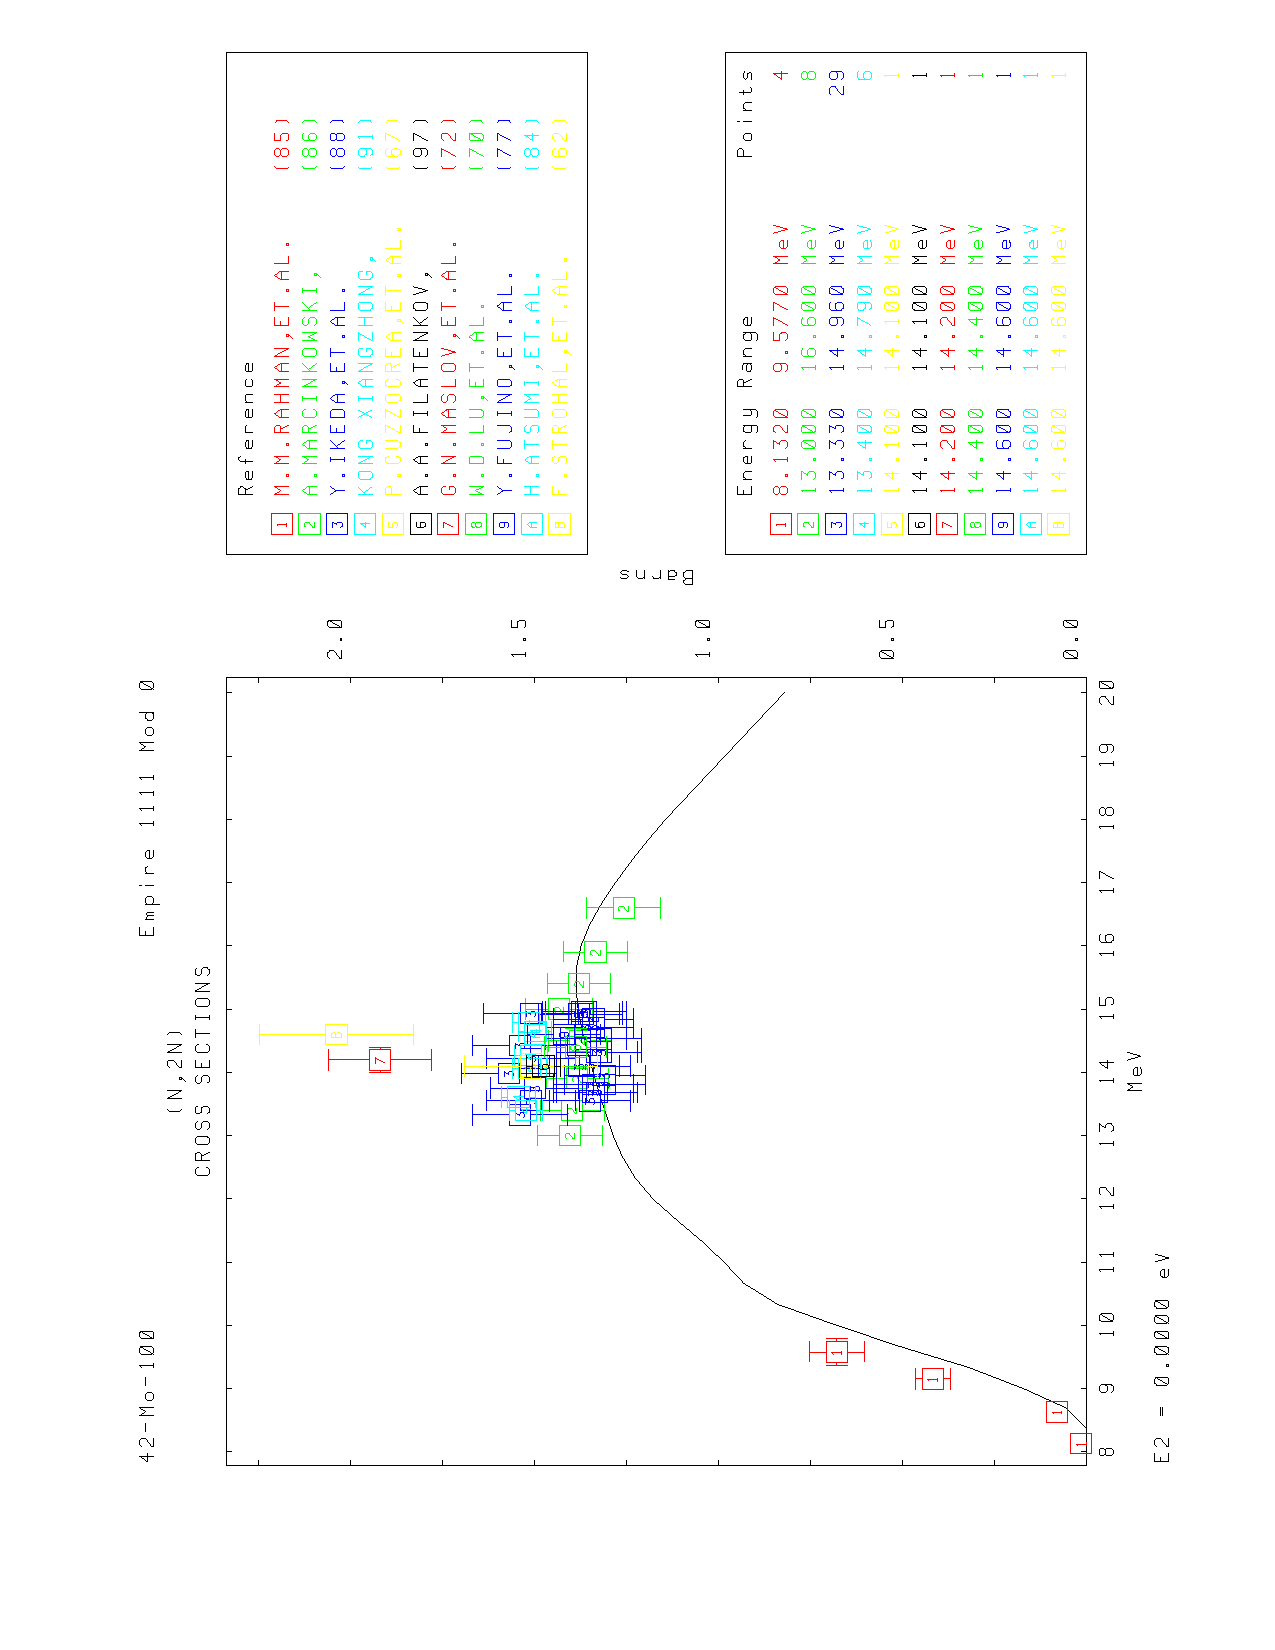
\includegraphics[width=0.9\textwidth,angle=-90]{figs/mo100n2n}
\par\end{centering}

\caption{\label{fig: 100Mon2n}Comparison of the experimental data extracted
from the EXFOR library with the results of EMPIRE calculations using
default parameters. This plot is produced automatically when running
EMPIRE with the \emph{run} script or clicking the Run+Format+Plot
button in GUI mode.}

\end{figure}



\subsection{ZVView}

The plotting capabilities of EMPIRE rely on  the graphic package 
ZVView\index{ZVView} by Zerkin~\cite{ZVView}.
This software is operated from the EMPIRE GUI and produces publication
quality plots. The scale can be changed, selected data sets can be
excluded from the plot, and data points values displayed; changes
can also be made to the plot title, subtitle, symbols and colors,
data fitting, smoothing and others. Plots can be exported to the PostScript
or encapsulated PostScript format for inclusion in the \LaTeX{} document. 

Contrary to PLOTC4, ZVV plots are not generated automatically. The
user has to select a desired reaction from the EMPIRE GUI (\fbox{Select MT and $>$}
button or type MT number in the entry box at the bottom of the GUI)
and click on the \fbox{ZVV} button. Internal scripts and components
of the ZVView\index{ZVView} package process the ENDF and \emph{{*}.c4}
files to produce the \emph{{*}-MT.zvd} file, which is then displayed
with the ZVView. 

ZVV plots can also be combined to include different reactions on the
same graph. Clicking on the \fbox{Merge ZVV} button will open the
terminal with a list of all ZVV plots available in the \emph{work}
directory. The user may select any number of them to be included in
a single plot. Usually, the plot title has to be set within the ZVView\index{ZVView}
environment before saving.

Additional functionality is offered by the ZVView GUI (see Fig. \ref{fig:GUIZVV}),
which permits comparison of up to three calculations (or ENDF files),
and experimental data (see Fig. \ref{complot1}, \ref{complot2} and
\ref{complot3}). It is primarily intended as a tool for checking
the effect of different options used in the calculations or comparing
the results with other evaluations. Usually, one would undertake a
set of calculations and use the script \emph{store} to move (or copy)
all the relevant files to a specified directory. For example, to store
the project with root-name {}``fe56'' in a \emph{case1} directory,
one should type: 

\begin{quote}
\texttt{../scripts/store ../case1 fe56 }
\end{quote}
inside the \emph{work} directory (note that \emph{case1} will be on
the same level as \emph{work}). Thus, the working directory is free
to run new calculations with the modified input. These results can
again be stored in another directory (e.g., \emph{case2}) and the
third set of calculations executed in the \emph{work} directory. If
experimental data are to be plotted, the \emph{{*}.c4} file with the
same root-name should be present in the first directory, which is
ensured if EXFOR data were extracted by EMPIRE. Clicking the \fbox{Compare ENDF file}
button of the EMPIRE GUI launches ZVV GUI, as shown in Fig. \ref{fig:GUIZVV}.
Note that the root-name of the project and \emph{work} directory are
by default transferred to ZVV GUI. Comparisons can be made by pointing
the ``File 2:'' and ``File 3:'' fields
to other files containing ENDF formatted data (e.g., stored in \emph{case1}
and \emph{case2} directories). We stress that while the first set
is referenced through its directory and default names \emph{{*}-s.endf}
and \emph{{*}.c4} the other two are identified by respective arbitrary
file names. An arbitrary suffix identifying the comparison plots and
labels for each curve should be entered in the respective fields.
At this stage the system is ready to create the requested plots (\fbox{Create selected}
button). One can also choose to create all plots at once (\fbox{Create all}
button), although they can be viewed one by one or merged together.
ZVV GUI can also be used to create simple ZVV plots by replacing the
EMPIRE GUI function. Leaving labels related to ``File 2:'' and ``File 3'' fields and suffix blank, simple ZVV
plots can be created for all the reactions with just one mouse click.
Setting the project field to ``*'' (without ``'') creates plots for all reactions and targets for which
\emph{{*}-s.endf} files exist in the \emph{work} directory. This comparison
capability is not limited to the EMPIRE results; any evaluated file
in the ENDF format can be compared with another ENDF file or with
EMPIRE calculations, providing that the first file is named (or linked)
as \emph{{*}-s.endf} and placed in the \emph{work} directory.

%
\begin{figure}[top]
\begin{centering}
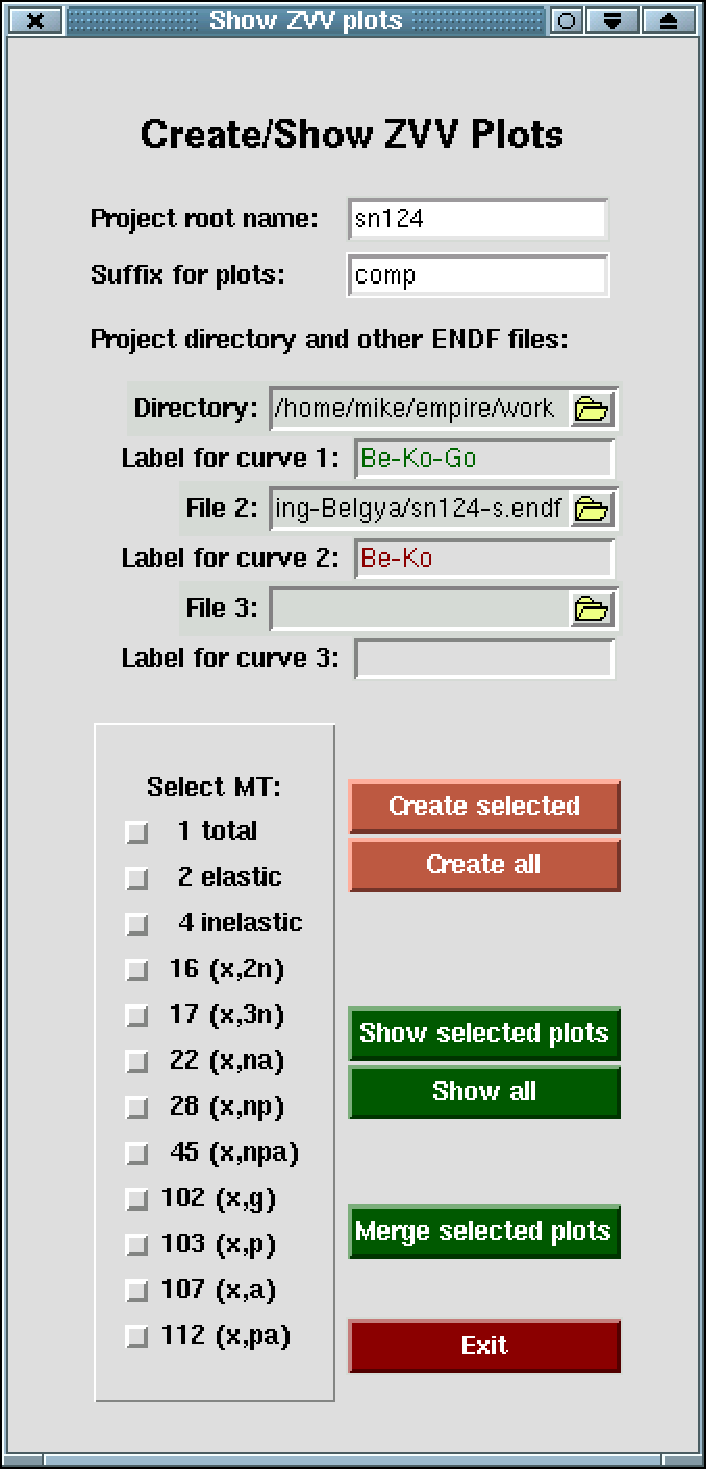
\includegraphics[height=1.1\textwidth]{figs/ZVVGUI}
\par\end{centering}

\caption{\label{fig:GUIZVV}Graphic User Interface to ZVView\index{ZVView}
to compare up to three calculations (or ENDF files) and merge different
reactions on a single ZVV plot.}

\end{figure}


As a rule, only the ENDF-formatted files can be plotted with PLOTC4\index{PLOTC4}
or ZVView\index{ZVView}. This choice is not only a matter of convenience
but was deliberately selected to validate the final (ENDF-formatted)
product. The only exception to this rule is provided by the \fbox{Create ZVV}
GUI button, which allows the user to construct and plot any excitation
function directly from the EMPIRE output. Hence, the user has to supply
a string which unambiguously identifies the cross section. The \emph{gawk}
script scans EMPIRE output (\emph{{*}.lst}) for the lines containing
the specified string and extracts a number (cross section) followed
by the ``mb'' string along with the respective incident
energy value. The results are sent to ZVView\index{ZVView} for plotting. 


% \subsection{PLOTC4}
% 
% The X4TOC4\index{X4TOC4} and PLOTC4\index{PLOTC4} codes have been
% extended and incorporated into the ENDF Data Verification Package
% (ENDVER) by Trkov and Cullen to plot angular distributions and double-differential
% cross sections~\cite{ENDVER}. A typical example of such a plot is
% shown in Fig. \ref{fig:93Nb-ddx}. Since plotting might be very time
% consuming (e.g., in the case of 238-U) by default plots are no more
% generated at the end of each run, but have to be explicitly requested
% by running \emph{../scripts/plot} script or by selecting 'Plotting
% (PLOTC4)' check box in GUI (Main1). The layout and contents of the
% plots can be customized by editing the PLOTC4 input file available
% through the Graphic User Interface (GUI). 
% 
% %
% \begin{figure}[top]
% \begin{centering}
% \includegraphics[width=0.7\textwidth,angle=-90,bb = 0 0 200 100, draft, type=eps]{nb93-KoBeGo-90.eps}
% \par\end{centering}
% 
% \caption{\label{fig:93Nb-ddx}Calculated neutron emission spectrum from $^{93}$Nb
% at 90$^{\circ}$ and incident energy of 14.1 MeV compared with the
% experimental data using PLOTC4\index{PLOTC4}. The Ko-Be-Go set of
% input parameters has been used in the calculations (see p. \pageref{Ko-Be-Go}).}
% 
% \end{figure}



\section{Plans for further development}

Following extensions are foreseen in the future releases of the EMPIRE
code:

\begin{enumerate}
\item Inclusion of isospin,
%\item Microscopic p-h level densities\index{p-h level densities} (routine
%  exists),
%\item Moldauer method for widths fluctuation correction, 
\item Width fluctuation correction for reactions on excited targets,
\item Improved parametrization of the elastic enhancement factor,
\item ENDF-formatting of primary gammas.
\item Improved description of direct reactions (e.g. breakup, pickup, etc.)
  for reactions with incident complex particles
  (e.g. deuteron, triton and $^3$He),
\item Implement particle decay of discrete levels that is relevant
  for the treatment of direct reactions (e.g. 12C(n,n+3$\alpha$) ) 
  in the outgoing channels.
\item Inclusion of heavy-ion optical potential (Sao Paulo potential).
\end{enumerate}

\part{WORKING NOTES} \label{Chap:work}


\chapter{Avoiding problems}

Consideration and observation of the following remarks will help to
avoid problems when running the EMPIRE code:

\begin{itemize}
\item Each modification of the EMPIRE input file ({*}.\emph{inp}) that involves
a change of projectile, target, or the number of emitted particles
must be followed by the execution of the \emph{clean} script in order
to remove input/output files that do not match the new case. One should
keep in mind that \emph{clean} will also remove all the files that
might have been modified manually (such as \emph{{*}.lev, {*}-omp.dir},
etc.). If these files are compatible with the new input and are to
be preserved they have to be renamed by adding a prefix before executing
the \emph{clean} script.
\item Any serious calculations should be preceded by a test run using FITLEV
set to a positive value in order to check the completeness of the
discrete level schemes and their consistency with the level densities\index{level densities}.
Such calculations should be repeated after each change of the input
file ({*}.\emph{inp}) that requires running the \emph{clean} script
(see above). Calculation times for such runs are very short. 
\item If the ENDF option is selected, the incident energies should be in
increasing order.
\item Log files \emph{{*}.war, {*}.x42c4\_errs} and \emph{empend.log} should
be checked for possible warnings and error messages.
\item Irregularities in the excitation functions such as (n,2n) or (n,p)
are usually due to improper level density\index{level density} parametrization
(check cumulative plots of discrete levels) or to the overestimated
MSD\index{MSD} contribution (check response functions and ensure
that the levels to which they are adjusted are actually the collective
ones).
\item Irregularities in the increasing part of the excitation function for
inelastic scattering are usually due to insufficiently dense mesh
of incident energies.
\end{itemize}

\chapter{Fitting discrete levels}

Running EMPIRE with the FITLEV option is strongly recommended before
any cross section calculations are attempted. This allows a check
of whether the discrete level schemes for the involved nuclei are
complete and consistent with the level density\index{level density}
parametrization. If the whole package is properly installed, plots
of cumulative number of levels will be stored in the \emph{{*}-cum.ps}
file and can be inspected in the PostScript viewer (ghostview) by
clicking on the \fbox{Levels} button in the ``Plots:''
section of the GUI. Two somewhat extreme examples of such plots are
shown in Fig. \ref{fig: badfit} and \ref{fig: goodfit}. Fig. \ref{fig: badfit}
demonstrates 10 levels in $^{96}$Pd, which could not be matched with
the level densities, which usually happens when the levels are over
extend. Then, levels that were not detected experimentally are missing
in the spectrum, and the resulting high energy end of the cumulative
plot is too low. Missing levels are more likely in the high-energy
region of the spectrum and reducing the number of levels considered
may restore agreement; neglecting the highest 4 levels in $^{96}$Pd
leads to a reasonable fit, as shown in the Fig. \ref{fig: goodfit}.
Graphical representation helps to identify the level at which cumulative
plot starts to bend, and levels lying above this point should be excluded
from consideration. One should edit .\emph{lev} file and decrease
$N_{max}$ parameters (6$^{th}$ entry in the first line of a given
isotope section) to remove levels in excess. The next step after the
modified \emph{{*}.lev} file is saved is to rerun the code and check
whether the applied cuts are sufficient. If this is not the case,
the whole procedure should be repeated and further levels removed.
Note, levels are only removed from the local file of the specific
case being calculated, and that \emph{Zxxx.dat} files in the parameter
library are not affected.

%
\begin{figure}[top]
\begin{centering}
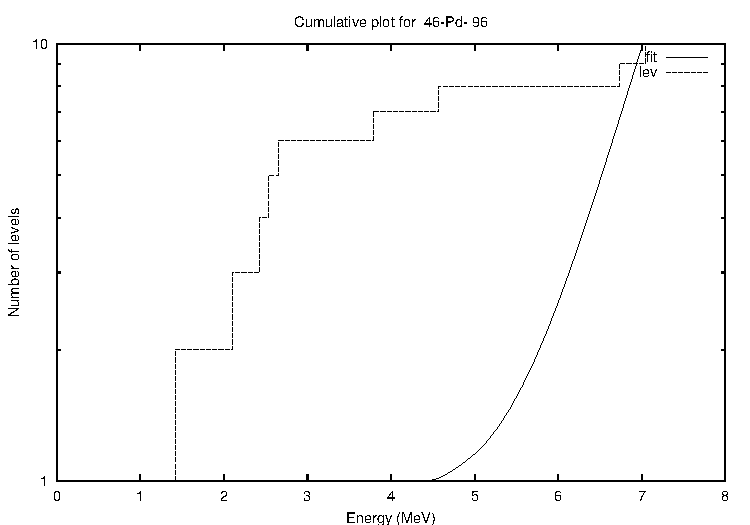
\includegraphics[width=0.7\textwidth]{figs/bad-fitliv}
\par\end{centering}

\caption{\label{fig: badfit} Cumulative plot of 10 discrete levels in $^{96}$Pd
which could not be reproduced by the level density\index{level density}
calculations (EMPIRE-specific level densities with default parametrization
were used).}

\end{figure}


%
\begin{figure}[top]
\begin{centering}
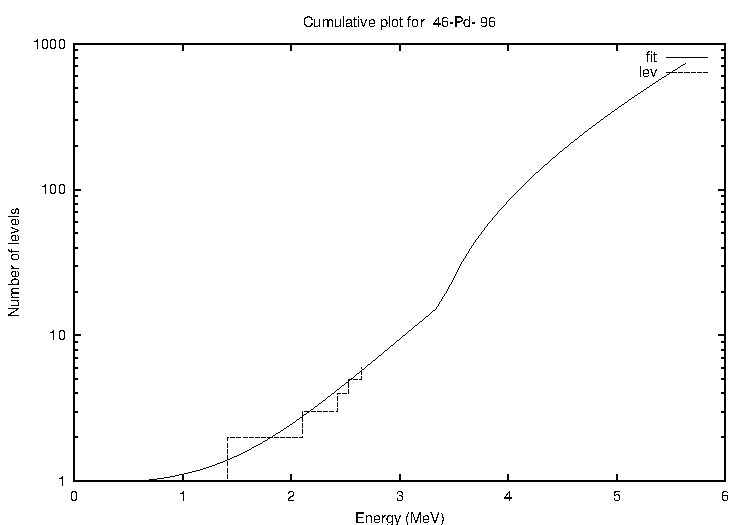
\includegraphics[width=0.7\textwidth]{figs/good-fitliv}
\par\end{centering}

\caption{\label{fig: goodfit}Same as Fig. \ref{fig: badfit} but after restricting
the fit to the first 6 levels only. Note the difference of two orders
of magnitude in the level densities\index{level density} around 6
MeV.}

\end{figure}

There are no restrictions on the contents of the input file ({*}.\emph{inp})
used for displaying the cumulative plots except that the FITLEV record
must be included with VAL different from 0. Dispositions that do not
consider level densities are ignored as the code exits after the plots
are completed without performing any cross section calculations.

\chapter{Handling OM potentials\index{RIPLomp}}

Interface to the RIPL optical model segment has been developed by
Capote. This interface allows the use of any type of Optical Model
Potential (OMP) contained in the library (including dispersive ones)
by specifying the OMP catalog number in the optional input (list of
available OMPs can be accessed from the EMPIRE GUI through the menu \fbox{Help}
$\Rightarrow$ \fbox{RIPL-omp})). The OMPOT record contains two numerical
values in addition to the usual keyword. The first value is the OMP
catalog number entered with a \textbf{negative} sign, which indicates
that the potential is going to be taken from RIPL\index{RIPL} rather
than from the internal sets coded in EMPIRE. The second value defines
the type of particle. For example,

\begin{description}[style=multiline,leftmargin=5cm]
\item [{OMPOT~~~-401.~~~~~~1}] selects RIPL Wilmore-Hodgson
global potential (RIPL number 401) for neutrons,
\item [{OMPOT~~-4004.~~~~~~2}] selects RIPL CC potential for
protons (to be used for $^{197}$Au only).
\end{description}
The code will create \emph{{*}-omp.ripl} file containing parameters
for the selected potentials for all nuclei and particles involved
in the calculations. This file can be edited in order to adjust OMP
parameters extracted from RIPL\index{RIPL}. RIPL Coupled-Channels
Optical Model Potentials (CC-OMP) include collective discrete levels
and related deformations, and thus the \emph{{*}-omp.ripl} contains
all information needed to run Coupled-Channel (CC) calculations. 

The ECIS06\index{ECIS} module, along with the RIPL\index{RIPL} interface,
bring into EMPIRE an easy access to a large number of optical model
potentials. However, the related input keywords (DIRECT, DIRPOT and
OMPOT) must be used with considerable care. In the following, we will
explain different combinations of these keywords, focusing on the
use of optical model parameters within EMPIRE. To this end we will
discuss several examples of neutron induced reactions on a spherical
nucleus ($^{54}$Fe) with dynamic deformation (vibrational case),
and on a deformed one ($^{153}$Eu) with static deformation (rotational
case). The general input file may contain the following lines:

\vspace{0.3cm}


\begin{flushleft}
\begin{tabular}{lrcl}
\texttt{DIRECT} & \texttt{x.} &  & ~call ECIS for CC, CC full or DWBA\tabularnewline
\texttt{DIRPOT} & \texttt{~~-xx.} &  & ~RIPL OMP for direct (inelastic) channel\tabularnewline
\texttt{OMPOT} & \texttt{~~-xx.} & \texttt{~~z} & ~RIPL OMP for particle z\tabularnewline
\end{tabular}
\par\end{flushleft}

\vspace{0.3cm}


In the following examples we use case-specific file names as created
when script or GUI modes are used to run the code. We recall that
the correspondence between the case specific names and those generated
by the code is the following:

\begin{description}[style=multiline,leftmargin=3cm]
\item [{\emph{{*}-omp.dir}}] $\Longleftrightarrow$ \emph{OMPAR.DIR }
\item [{\emph{{*}-omp.ripl}}] $\Longleftrightarrow$ \emph{OMPAR.RIPL}\index{RIPL} 
\item [{\emph{{*}-lev.col}}] $\Longleftrightarrow$ \emph{TARGET\_COLL.DAT }
\end{description}
\noindent with ``*'' standing for the actual root-name
of the file. 


\section{DWBA\index{DWBA} with RIPL OMP}

Apply the DWBA model to the spherical vibrational nucleus $^{54}$Fe.
Our goal is to perform calculations using default spherical RIPL potentials
for all channels, but including inelastic scattering calculated by
ECIS06\index{ECIS} with the DWBA\index{DWBA} option using RIPL spherical
OMP catalog number 10. The input file must contain two lines: 

\begin{description}[style=multiline,leftmargin=3cm]
\item [{DIRECT}] 3. 
\item [{DIRPOT}] -10. 
\end{description}
Resulting OMP files: 

\begin{description}[style=multiline,leftmargin=3cm]
\item [{\emph{{*}-omp.ripl}}] default RIPL OMP used for all the channels
in the HF\index{Hauser-Feshbach} calculations. 
\item [{\emph{{*}-omp.dir}}] spherical OMP employed in the DWBA\index{DWBA}
calculations of the inelastic scattering to collective discrete levels,
in this case RIPL\index{RIPL} OMP potential catalog number 10.
\end{description}
We can adjust the inelastic scattering cross sections in subsequent
runs by changing OMP inside the \emph{-omp.dir} file and/or by changing
dynamic deformations inside the \emph{{*}-lev.col} file (initial deformation
values are 0.15 for quadrupole and 0.05 for octupole vibrations).


\section{Coupled-Channels\index{Coupled-Channels} with RIPL spherical OMP}

Our goal is to perform calculations for $^{54}$Fe using default RIPL
potentials for all the channels, but including inelastic scattering
calculated by the ECIS06\index{ECIS} CC option using RIPL spherical
OMP potential catalog number 10. The input file must contain 2 lines: 

\begin{description}[style=multiline,leftmargin=3cm]
\item [{DIRECT}] 1. 
\item [{DIRPOT}] - 10. 
\end{description}
Resulting OMP files: 

\begin{description}[style=multiline,leftmargin=3cm]
\item [{\emph{{*}-omp.ripl}}] RIPL OMP used for all the channels in the
HF\index{Hauser-Feshbach} calculations. 
\item [{\emph{{*}-omp.dir}}] spherical OMP employed for the CC calculations
of the inelastic scattering to collective discrete levels, in this
case RIPL\index{RIPL} OMP catalog number 10.
\end{description}
We can adjust the inelastic scattering cross sections in subsequent
runs by changing OMP inside the \emph{{*}-omp.dir} file or by changing
dynamic deformations inside the \emph{{*}-lev.col} file.


\section{Coupled-Channels\index{Coupled-Channels} with RIPL CC
OMP for inelastic scattering}

We intend to perform calculations for $^{153}$Eu using RIPL spherical
potential catalog number 221 for all neutron channels (local potential
for $^{153}$Eu) except the inelastic channel, for which we are going
to calculate cross sections with the CC method using the RIPL\index{RIPL}
CC-OMP potential catalog number 2004. The input file must contain
3 lines: 

\begin{description}[style=multiline,leftmargin=3cm]
\item [{DIRECT}] 1. 
\item [{DIRPOT}] -2004. 
\item [{OMPOT}] -221.~~~~~~~ 1
\end{description}
Resulting OMP files: 

\begin{description}[style=multiline,leftmargin=3cm]
\item [{\emph{{*}-omp}.\emph{dir}}] deformed (CC) OMP employed for the
CC calculations of the inelastic channel, (RIPL\index{RIPL} potential
catalog number 2004 in this case (contains collective levels and respective
deformations)). 
\item [{\emph{{*}-omp.ripl}}] RIPL spherical OMP catalog number 221 used
in the HF calculations of neutron channels.
\end{description}
The inelastic scattering cross sections can be adjusted in subsequent
runs by changing OMP inside the \emph{{*}-omp}.\emph{dir} file or
by changing the static deformation of the ground state band inside
the same file. We are using a true CC-OMP from RIPL\index{RIPL} and
collective levels are stored together with the potential parameters
inside the \emph{{*}-omp}.\emph{dir} file. 


\section{Complete Coupled-Channels\index{Coupled-Channels} with RIPL CC OMP
for inelastic scattering}

Our aim is to perform exact calculations for $^{153}$Eu using
default EMPIRE potentials for all charged particle channels and the
RIPL spherical OMP catalog number 221 (local potential for $^{153}$Eu)
for all neutron channels except inelastic, for which we are going
to calculate cross sections and transmission coefficients consistently
using the CC method and the RIPL\index{RIPL} CC-OMP catalog number
2004. The input file must contain three lines: 

\begin{description}[style=multiline,leftmargin=3cm]
\item [{DIRECT}] 2. 
\item [{DIRPOT}] -2004. 
\item [{OMPOT}] -221.~~~~~~~ 1
\end{description}
Resulting OMP files are: 

\begin{description}[style=multiline,leftmargin=3cm]
\item [{\emph{{*}-omp.ripl}}] CC-OMP employed for the CC calculations of
the fusion and inelastic channels (RIPL\index{RIPL} CC-OMP number
2004 (contains collective levels and respective deformations)). In
addition, the file contains RIPL S-OMP number 221 employed for all
other neutron channels except inelastic. 
\item [{\emph{{*}-omp.dir}}] is not created since a true CC-OMP is used
consistently and all relevant parameters are contained in the \emph{{*}-omp.ripl}
file.
\end{description}
The inelastic scattering cross sections can be adjusted in subsequent
runs by changing either S-OMP inside the \emph{{*}-omp.ripl} file
or the static deformation of the ground state band inside the \emph{{*}-lev.col}
file (initial value is the experimental g.s. quadrupole deformation).
Note that the CC-OMP and the CC method are also used for the calculation
of the fusion cross section.


%\chapter{Use of level densities}


\chapter{Effects of parameter modifications}

The parameter libraries and internal systematics contained in the
EMPIRE code perform reasonably well in reproducing cross sections
for major neutron induced reactions up to 20 MeV. However, one can
not expect that global parametrization will provide perfect fits to
all channels and at all incident energies. Weak reaction channels
may differ substantially from the experimental data. In view of the
uncertainties associated with the model parameters, certain adjustments
were made in order to fit measured cross sections. Guidance is given
below on parameter tuning, indicating the most sensitive methods and,
if possible, describing the effect of their modification.

It is strongly recommended that various available options in the code
are exploited before any attempt is made to change the parameters.
This guarantees that physically meaningful parameters are used. For
example, the user may try different optical model potentials, various
formulations and/or parameterizations of level densities\index{level densities}
and eventually different preequilibrium models. These attempts should,
at least, provide the user with the best starting point for parameter
adjustment. We note that various options may provide very different
results as illustrated by the following three sets of calculations:

\begin{figure}[top]
\begin{centering}
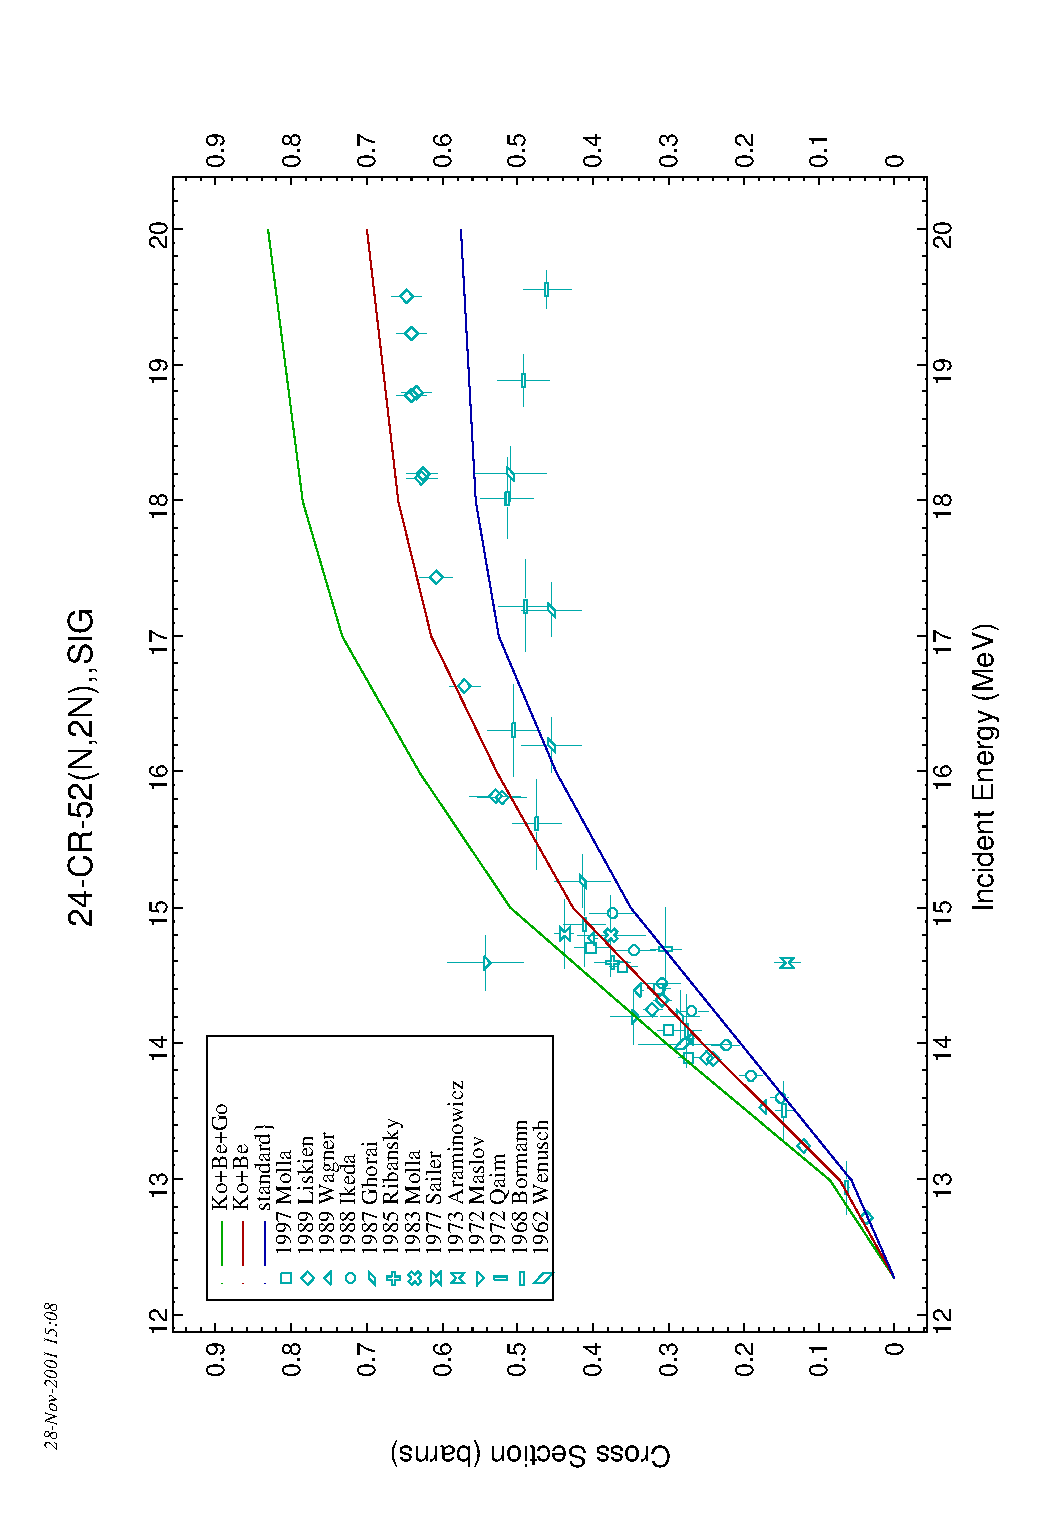
\includegraphics[width=0.7\textwidth,keepaspectratio,angle=-90]{figs/cr52n2n}
\par\end{centering}

\caption{\label{complot1}Comparison of experimental data with results calculated
using three sets of parameters for the $^{52}$Cr(n,2n) reaction (see
text).}

\end{figure}


\begin{description}[style=multiline,leftmargin=3cm]
\item [{standard}] Wilmore-Hodgson S-OMP for neutrons and Becchetti-Greenlees
for protons, EMPIRE-specific level densities with internal systematics,
and discrete levels up to N$_{max}=10$ (note that in EMPIRE-3.1
Koning-DeLaroche potential is a standard),%

\item [{Ko-Be}] Koning-DeLaroche S-OMP for neutrons and protons, discrete
levels up to the N$_{max}$ recommended by RIPL (limited to 40 by
the ENDF-6 format), and EMPIRE-specific level densities,
\item [{Ko-Be-Go\label{Ko-Be-Go}}] as above but using HFB\index{HFB}
microscopic level densities\index{level densities}\cite{HFBCS} instead
of the EMPIRE-specific ones.
\end{description}

Figs. \ref{complot1}, \ref{complot2} and \ref{complot3} show comparison
of the results obtained using the above sets of parameters in three
sample cases. Differences of a factor of 2 are observed, and therefore 

%
\begin{figure}[top]
\begin{centering}
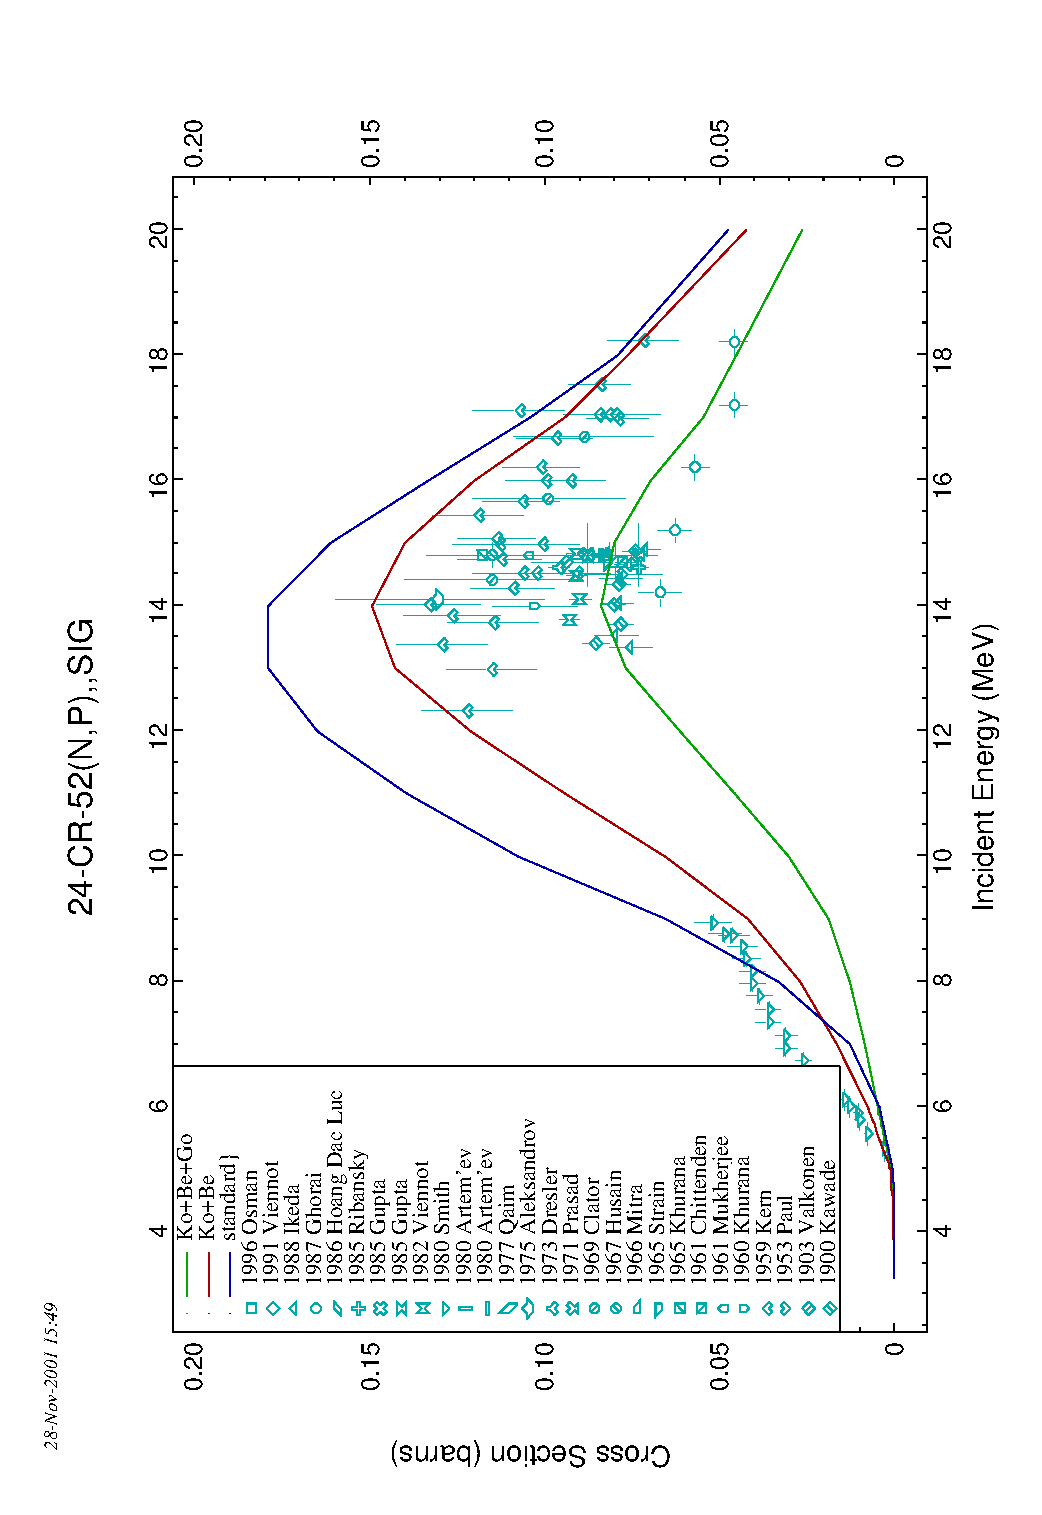
\includegraphics[width=0.7\textwidth,keepaspectratio,angle=-90]{figs/cr52np}
\par\end{centering}

\caption{\label{complot2}Comparison of experimental data with results calculated
using three sets of parameters for the $^{52}$Cr(n,p) reaction (see
text).}
\end{figure}
changing the default options may considerably improve the comparison
with experimental data. However, this approach may still not be sufficient
in some cases, and the next step would be to determine which reaction
mechanism is most likely to be responsible for the disagreement, remembering
that neutron capture below 10 MeV and the low energy part of the particle
spectra are essentially due to Compound Nucleus decay. The high energy
part of particle spectra is dominated by the preequilibrium emission,
and population of the collective discrete levels in inelastic scattering
arises mainly from the direct reactions. We also note that at incident
energies below 50 MeV the multiple-chance preequilibrium emission
is rather small and multiple particle emission is governed by the
statistical decay. The list below should help pinpoint the mechanism
that might be causing a problem:

%
\begin{figure}[top]
\begin{centering}
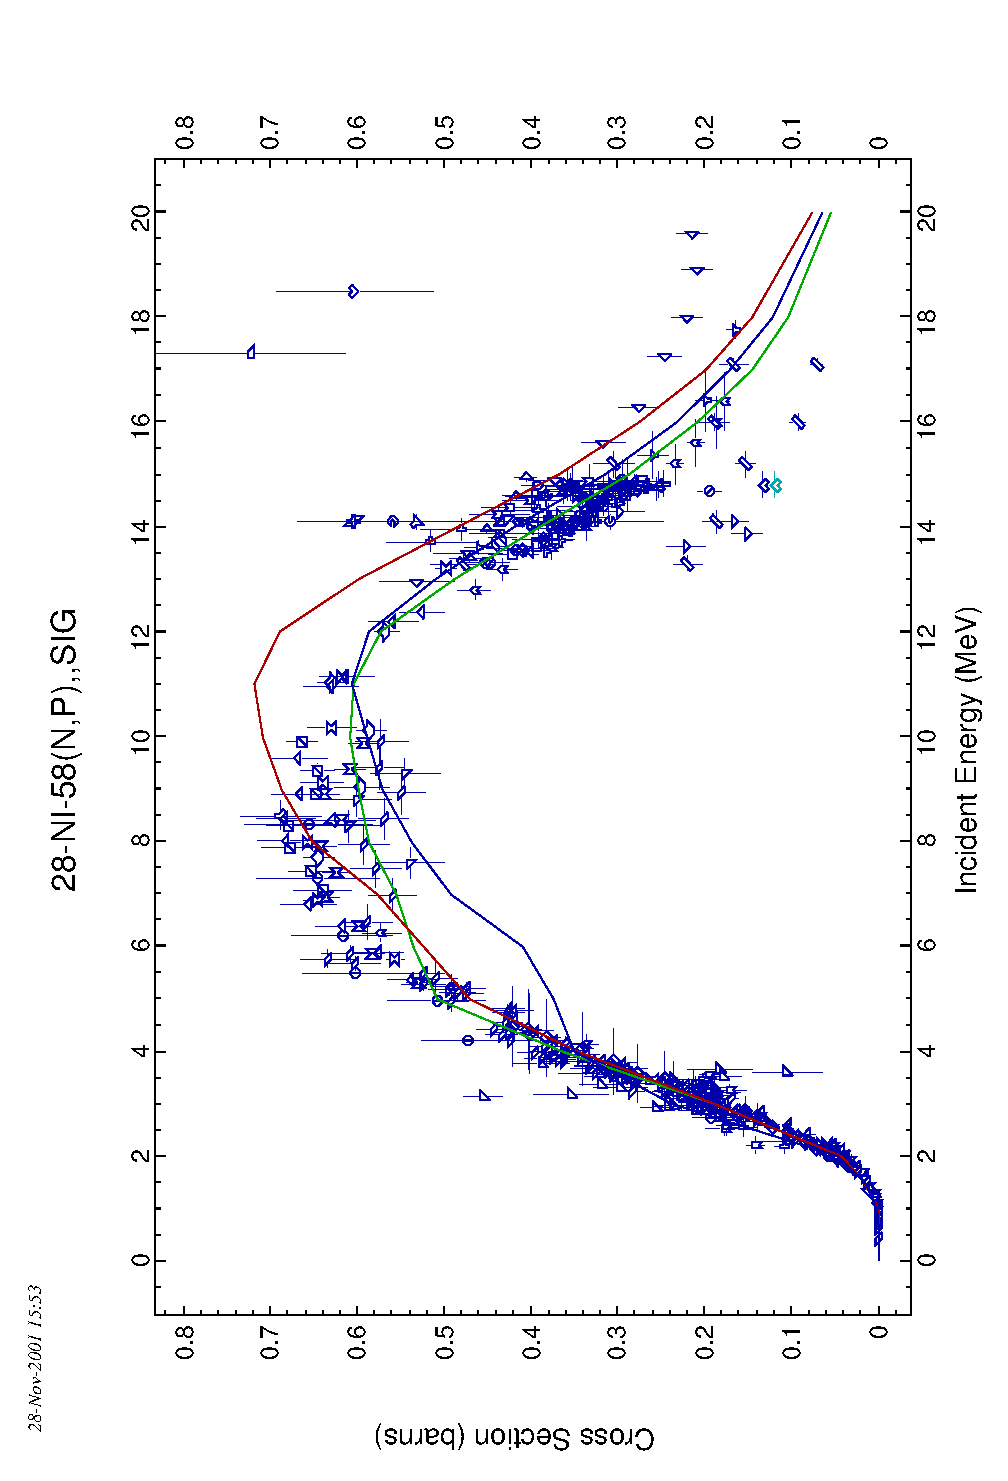
\includegraphics[width=0.7\textwidth,keepaspectratio,angle=-90]{figs/ni58np}
\par\end{centering}

\caption{\label{complot3}Comparison of experimental data with results calculated
using three sets of parameters for the $^{58}$Ni(n,p) reaction (see
text).}

\end{figure}


\begin{itemize}
\item \textbf{Nucleon spectra at high ejectile energies underestimated (overestimated)}
- these are usually related to the underestimated (overestimated)
preequilibrium emission.
\item \textbf{Tails of the inelastic scattering cross sections underestimated
(overestimated)} - again caused by too low (too high) preequilibrium
contribution. 
\item \textbf{Inelastic cross sections to discrete levels} \textbf{underestimated
(overestimated)} - lack of or too low (too high) contribution from
the direct reactions is the most likely reason. In case of under-estimation,
user should ensure that Coupled-Channel or DWBA\index{DWBA} option
is turned on (DIRECT=1, 2, or 3). Generally, the Coupled-Channel option
will provide higher cross sections than DWBA.
\item \textbf{Capture cross sections below 10 MeV} \textbf{underestimated
(overestimated)} - as mentioned before, the Compound Nucleus is responsible.
The discrepancy might be traced to $\gamma$-ray strength function
being too low being too low (too high) or to the ratio of level densities\index{level densities}
in the daughter nuclei and the Compound Nucleus being too low (too
high) ($\rho_{n}/\rho_{CN}$ - note that the neutron channel is usually
the main competitor). 
\item \textbf{Capture cross sections above 10 MeV} \textbf{underestimated}
- be sure that the exciton model PCROSS is turned on.
The preequilibrium emission of $\gamma$s (or the Direct-Semidirect
mechanism) is responsible for more than 90\% of the capture cross
section in this energy range.
\item \textbf{Cross sections} \textbf{underestimated (overestimated)} \textbf{in
all channels} - can be traced to an inadequate optical potential that
provides too low (too high) absorption cross section.
\item \textbf{Wrong total cross section} - obviously an inadequate optical
potential. 
\item \textbf{Wrong angular distributions for elastic scattering} - again
would assume an inadequate optical potential to be the main reason.
At low energies where few inelastic channels are open, there might
be a non-negligible contribution from the symmetric compound elastic,
which could be affected by the wrong $\rho_{n}/\rho_{CN}$ ratio.
\item \textbf{Cross sections for the $\alpha$-channel} \textbf{underestimated}
- for nuclei with masses larger than about 100, the discrepancy is
not due to wrong parameters but to the lack of a preequilibrium emission
of clusters in the present version of EMPIRE. One may compensate for
this deficiency by increasing level densities\index{level densities}
in the residue after $\alpha$ emission or by increasing the diffuseness
of the optical model potential for $\alpha$-particles. However, the
resulting parameters will be unphysical. Such an intervention may
only be justified for lighter nuclei, for which preequilibrium emission
of $\alpha$-particles is relatively unimportant. 
\item \textbf{Fission cross sections} \textbf{underestimated (overestimated)}
- for neutron induced fission, the current fission model coded in
EMPIRE is too crude. One may try to cure the problem by decreasing
(increasing) the fission barrier or increasing (decreasing) level
densities at the saddle point, but this should be considered as an
arbitrary fitting exercise without much physical meaning. Tuning fission
cross sections in the HI induced reactions will be discussed later
on.
\item \textbf{Excitation functions shifted in energy} - for nuclei far from
the stability line (typical for HI induced reactions), this effect
can be traced to incorrect binding energies (masses). A modest change
of binding energies (of the order of 0.5 MeV) can be justified as
being within the uncertainty of the theoretical masses. However, this
argument does not hold for nuclei close to the stability valley since
experimental nuclear masses are known with a rather high accuracy.
\item \textbf{Structure in the continuum part of the inelastic scattering
spectrum ``out of phase''} - this structure originates
from the MSD\index{MSD} contribution. When the spectrum does not
match experiment, the user may attempt to tune calculations by changing
the positions of collective levels to which the response functions
are fitted.
\item \textbf{Double-differential spectra for inelastic scattering to continuum
at small angles ($<40^{o}$) underestimated} - MSD\index{MSD} mechanism
is responsible for the major part of the cross section in this range.
Choosing the compressional form factor for the $l=0$ transfer (default
is the surface form factor) should bring substantial improvement.
In fact, from the physical standpoint this \emph{is} the factor that
should be used for the $l=0$ transfer. The different default is being
used due to the numerical instabilities that happen occasionally when
this physically-correct option is selected. 
\item \textbf{Wrong ratio between two competing channels (e.g., $\sigma$(n,n)
/$\sigma$(n,p))} - at low incident energies this ratio is governed
by the Compound Nucleus decay and may be distorted by an inappropriate
ratio of level densities\index{level densities} in the two competing
channels. Actually, the cross section ratio is approximately proportional
to the level density ratio in the respective residual nuclei. Also,
the optical model potential may have a significant effect. At higher
incident energies, the preequilibrium contribution starts to play
a role, and a reference for one of the preequilibrium channels may
provide a solution.
\item \textbf{Wrong slope of the increasing part of the excitation function}
- a crucial role is played by the discrete levels in the residual
nucleus and the optical model potential (transmission coefficients),
of which the discrete levels are easier to control. Changing the number
of accepted levels may effectively increase or decrease the available
phase space for the particular decay mode.
\item \textbf{Production of residues in HI induced reaction underestimated
(overestimated)} - for lighter nuclei in which the fission channel
is not dominant, the fusion cross section might be too small (or too
big). Competition between fission and particle emission may constitute
an additional source of error for the highly fissile (heavy) nuclei.
In such a case, decreasing (increasing) strength of the fission channel
is usually an effective way of increasing (decreasing) residue production. 
\end{itemize}
The mechanisms and parameters that are expected to be the most important
and effective in solving a particular problem have been noted in the
above discussion. However, we are always dealing with a complicate
interplay of different factors and in some cases the major sources
of error may differ from those indicated. However, the user should
be able to identify the most critical reaction mechanism or a key
input quantity in most cases, and be able to avoid a random search
for optimal parameters. 

So far we have discussed the symptoms and possible reasons for operational
problems. Knowing the disease, we should now look for the most appropriate
treatment. We will indicate those input parameters to which particular
models or input quantities (such as fusion, level densities and\index{level densities},
$\gamma$-ray strength functions) are most sensitive. However, parameters
not mentioned below may also influence the results. Generally, their
effect should be less pronounced but they might become one of the
key players in particular situations. In addition, these assessments
are complicated and most of the parameters are correlated; for example,
deficiencies in one parameter can be compensated by a change in another
leading to unrealistic values. Therefore, it is important to understand
the physical reason for a discrepancy and proceed accordingly, and
to fit all available observables rather than a single cross section.
Such an approach increases the user's confidence in the final results.
Finally, fitting a single experimental point that differs dramatically
from the calculated value can be dangerous, especially when the exercise
involves a strong channel. The experimental point might simply be
wrong. Such cases are known in the EXFOR library, either because of
an erroneous experiment or a compilation error. In particular, if
the experimental data fall well below the calculated cross section,
the user should check whether the measurement concerned the total
cross section for the reaction channel or the cross section to the
isomeric or ground state.

In the discussion that follows, we group parameters according to the
reaction mechanism or input quantity to which they are relevant, and
refer to them by keywords defined in the input description (see Section
\ref{sec: input}). 


\section{Fusion}

We have to distinguish between Heavy Ion (HI) and Light Ion ($A<5$) or nucleon
induced reactions. For HI induced reactions one may use following parameters to 
control fusion cross section:

\begin{description}[style=multiline,leftmargin=3cm]
\item [{FUSRED}] scales calculated fusion cross section with an arbitrary
factor to set the parameter directly to the desired value, but lacks
any physical significance and predictive power. Should be used as
the last resource unless the fusion cross section is known from a
more microscopic model or experiment. 
\item [{BFUS}] Fusion barrier height in the distributed barrier model $B_{fus}$
(Eq. \ref{distbarr}) is by default calculated by the CCFUS\index{CCFUS}
and used for the HI induced reactions only. Even a slight decrease
of the barrier height can produce a considerable increase of the fusion
cross section (and vice versa) when the incident energy (in CM) is
close to the barrier height. This effect tends to disappear at higher
incident energies. 
\item [{SIG}] SIGMA in the distributed barrier model (Eq. \ref{distbarr})
is by default set to $0.05B_{fus}$. Increase of SIGMA will also increase
the fusion cross section. Similarly to BFUS, the effect is most pronounced
at low energies and tends to disappear at higher values.
\item [{EXPUSH}] Extra-push energy (default value is 0) is very effective
at decreasing the HI fusion cross section when increased. Physically
justified for a fusion of massive systems.
\item [{CRL}] Critical \emph{l}-value for the HI fusion (Eq. \ref{Tlfus})
sets fusion cross section to the required value - much like FUSRED.
\item [{DFUS}] Diffuseness in the transmission coefficients of HI fusion
(Eq. \ref{Tlfus}) does not change the fusion cross section, but defines
the spin distribution. Larger DFUS, the higher the spins populated,
and this effect may contribute to an increase of the fission cross
section and resulting reduction in the evaporation residues.
\end{description}

There are fewer possibilities for nucleon or LI induced reactions  as the cross section 
for fusion (also referred as absorption or reaction)
 is calculated using the optical model. Users may try
different parameterizations available in the RIPL\index{RIPL} library
or internal OMP systematics. If this fails, increasing the imaginary
part of the OMP will increase the absorption cross section. However,
users are advised that blind modification of the OMP can easily produce
physically unrealistic results. 


\section{Coupled-Channels\index{Coupled-Channels} (ECIS\index{ECIS})}

CC calculations are most sensitive to the deformations of collective
levels, which can be adjusted by editing the \emph{{*}-lev.coll} file
(see Section \ref{lev-coll}). Actually, if the collective levels
are selected internally rather than taken from the RIPL\index{RIPL}
library along with the CC optical model potential, these deformations
\emph{should} be adjusted. The code sets them by default to the g.s.
deformation for the rotational model and to the arbitrarily fixed
values for the vibrational model. These values can only be considered
as a first guess. Increasing the band deformation for the rotational
model or dynamic deformations for the vibrational model results in
an increase of the calculated direct cross sections (opposite is true
if the deformations are decreased).

Adding more collective levels to the \emph{{*}-lev.coll} file will
generally increase the total direct cross section, and may result
in a substantial increase of the cross section to the introduced levels.
Generally, the overall effect is not very significant as high energy
levels are usually only weakly coupled. Substantial increase of the
direct cross section, especially for the highly deformed nuclei, can
be achieved by using the CC approach instead of DWBA\index{DWBA}.
As a rule, CC model \emph{should} be the preferred choice in such
cases.

Obviously, the cross sections calculated with the CC model are sensitive
to the OMP. The effect might be considerable but is difficult to predict
due to the large number of parameters involved. Generally, deeper
imaginary part of the OMP (especially the imaginary surface component)
will result in the higher cross sections.


\section{Multi-step Direct\index{MSD}}

The microscopic character of the MSD\index{MSD} model limits the
possibilities of influencing the results compared with the classical
models (such as the exciton model). A certain degree of flexibility
is provided by the pairing gap parameters (GAPP for protons and GAPN
for neutrons). The dependence is non-linear, and it is difficult to
predict the impact of any change. MSD\index{MSD} results are slightly
more sensitive to the EFIT parameters, which define the energies of
the collective levels to which response functions for different multipolarities
are fitted. Again, due to the non-linearity, the results of the change
are hard to predict, the effect has an oscillating character. However,
on average, decreasing the EFIT value for a given multi-polarity results
in an increase in strength for the $l$-transfer under consideration
and a higher MSD\index{MSD} cross section. We stress again that EMPIRE
sets EFIT values internally to the energy of the lowest discrete level
which can be coupled to the ground state with a given $l$ transfer
(except $l=0$ transfer for which the self-consistent value is taken
by default). This assignment might be erroneous if there happens to
be a non-collective and low energy level with a suitable spin. In
such a case, the EFIT value should be corrected manually by entering
the EFIT keyword with the proper energy of the true collective level.
Modifications in the EFIT values will generally affect the structure
observed in the MSD\index{MSD} spectra by shifting maxima to different
energies, and the user is advised to try first the self-consistent
values for EFIT before attempting any arbitrary modifications.

Substantial increases in the MSD\index{MSD} contribution at \emph{forward
angles} can be obtained by switching to the compressional form factor
for the $l=0$ transfer (COMPFF=1). As already mentioned before, this
option is physically sound and strongly recommended.

The last resource involves multiplying the response function by an
arbitrary factor through the RESNOR entry. Factors larger than 1 will
increase MSD cross sections, and values smaller than 1 will reduce
it. This procedure has no physical meaning and may eventually lead
to the MSD emission being larger than the absorption cross section. 


\section{Multi-step Compound\index{MSC} }

The most significant MSC\index{MSC} contribution to the nucleon spectra
is located between the Compound Nucleus (low energies) and the MSD\index{MSD}
contributions (middle-high energies). MSC mechanism accounts for about
20-30\% of the total emission at incident energies close to 10 MeV
and decreases with the increasing incident energy. Therefore, one
should not expect too much from tuning this mechanism. Similarly to
MSD, the user's freedom to modify MSC is rather limited. The parameters
that have the largest effect are as follows:

\begin{description}[style=multiline,leftmargin=2cm]
\item [{GDIV}] Single particle level densities defining particle-hole level
densities\index{p-h level densities} in MSC\index{MSC} set to A/13
by default. Increasing (decreasing) GDIV will result in a higher (lower)
MSC cross section. Note that increasing GDIV is justified for nuclei
close to the magic numbers, as their level densities are significantly
lower. 
\item [{TORY}] Ratio of the cross sections for unlike and like nucleon-nucleon
interaction (e.g., $\sigma_{np}/\sigma_{nn}$). Can be used for adjusting
the relative share between neutron and proton emission. The default
value of 4, as derived from the free nucleon scattering, is generally
accepted, although some doubts have been expressed as to whether the
free scattering value should be applied to the scattering inside nuclear
matter. Increasing (decreasing) this parameters will favor (suppress)
the charge exchange channel.
\item [{D1FRA}] Ratio of the GDR spreading width to the total GDR width
(default: 0.8) is relevant to $\gamma$-emission only. While there
is not much room for increase, decreasing the ratio will also reduce
the already low $\gamma$-emission through the MSC\index{MSC} mechanism.
\end{description}


\section{Level densities}

The variety of nuclear level densities\index{level densities} available
in EMPIRE calls for additional guidance on their use. Only three options
are recommended: Empire-specific, Gilbert-Cameron (GC) and HFB\index{HFB};
all remaining options (such as ROCOL with level density parameter
\emph{a=A/8)} are included for comparison but their accuracy is much
lower than the three recommendations. The GC level densities, especially
when adjusted to known experimental data, may be the most accurate
at excitation energies up to the neutron binding and slightly above.
However, GC level densities do not lend themselves to extrapolation
to higher excitation energies and to nuclei far from the stability
line. Energy extrapolation in GC might be dangerous because of the
collective effects which are implicitly contained in the level density
parameter \emph{a}. While this can be an acceptable approximation
at low excitation energies for which level densities are fixed by
fitting experimental data (discrete levels and neutron resonance spacings),
there is no physical justification for extending such a treatment
to higher energies. In fact, collective effects, as implicitly accounted
for in the GC approach, increase exponentially with excitation energy
instead of decreasing and eventually disappearing. In this respect,
EMPIRE-specific and microscopic HFB\index{HFB} densities behave
properly and should be preferred at excitation energies well above
neutron binding. 

EMPIRE-specific level densities\index{level densities}, in addition
to explicit treatment of the collective effects and their damping,
also include the effects of dynamic deformation, which is induced
by the rotation of a nucleus at high spin. This deformation affects
level densities through the modification of nuclear moments of inertia.
The yrast line is taken into account by setting level densities to
zero whenever the thermal energy available for single particle motion
is negative. Thermal energy is calculated as the difference between
the total excitation energy and the energy needed for rotation. Spin
and energy ranges are also formally unlimited in the EMPIRE-specific
level densities. These features make the approach particularly suited
for the heavy ion and high-energy nucleon-induced reactions. On the
other hand, EMPIRE-specific level densities are fitted to the experimental
data in a manner similar to the GC, suggesting that their predictions
at low energies should be comparable to those of GC or even better
due to the use of the BCS\index{BCS} model below critical energy.
Therefore, EMPIRE-specific level densities\index{level densities}
are generally recommended, and are used as a default in the EMPIRE.

However, EMPIRE-specific level densities suffer the same uncertainty
as GC when extrapolating from the stability line, because both relay
on experimental parameterization of the level density parameter \emph{a},
which is only possible for stable or close to stable nuclei. For nuclei
far from the stability line, the HFB\index{HFB} densities based
on realistic schemes of single particle levels offer higher reliability.
The physics involved in this approach is clearly superior to the treatment
used in the two models discussed above, which makes HFB densities
more suitable for extrapolation. In addition, the tabulated values
provided by Goriely for RIPL\index{RIPL}-2 and available in EMPIRE
were adjusted to the same experimental data as the other two phenomenological
approaches. Therefore, results of the HFB model at low energies
should not differ significantly from those provided by the GC or EMPIRE-specific
models. Comparisons of cross section calculations for about 300 reactions
on targets from $^{40}$Ca to $^{208}$Pb show that microscopic level
densities\index{level densities} can compete with the phenomenological
ones to the extent that makes them the preferred choice far from the
stability line. On the other hand, one should keep in mind that tables
of level densities are limited to excitation energies below 150 MeV
and spins up to 30$\hbar$, which prevents their use for the Heavy
Ion induced reactions well above the Coulomb barrier. 




The Hauser-Feshbach results are very sensitive to the level densities\index{level densities},
and more precisely to their ratio in the neighboring nuclei. Generally,
changing level densities is the most effective way of adjusting cross
sections. As mentioned at the beginning of this Section, various formulations
of the level densities provided in EMPIRE should be considered with
their default parameterization first. Only if this exercise does not
produce sensible results should the user attempt to vary the model
parameters. The three recommended and most accurate models are (i)
EMPIRE-specific, (ii) Gilbert-Cameron, and (iii) HFB\index{HFB}.
All of them are fitted to match the discrete levels. While the pre-calculated
HFB level densities can not be modified, EMPIRE and Gilbert-Cameron
offer more significant flexibility. First of all, they are affected
by the number of discrete levels in the calculations (it is assumed
that cumulative plots had already been checked for consistency using
the FITLEV option). Generally, adopting fewer levels increases the
level densities between the last discrete level and neutron binding
energy, and considering more levels tends to decrease level densities\index{level densities}
in the same region (see Fig. \ref{fig: badfit} and \ref{fig: goodfit}).
However, this general statement may not hold in cases with strong
irregularities in the cumulative plots. Extending the discrete level
scheme too far involves a risk of including the region with missing
levels which would lead to an unphysical reduction of level densities.
The new RIPL library of discrete levels contains estimates of the
completeness of the scheme (N$_{max}$), which is used by EMPIRE as
a default. These values have been compared with the EMPIRE level densities
(i) and (ii) and were found to be compatible in about 75\% of cases.
The user should decrease N$_{max}$ in the remaining 25\%. If this
reduction is insufficient the discrete level region may extend too
far. Another extreme involves too few levels, in which there is a
risk of fitting level densities to a bunch of collective levels that
are shifted toward lower energies because of their collective nature.
The resulting level densities might be considerably overestimated. 

Changing the level density models and the number of discrete levels
may fail, and the user may be forced to adjust the level density parameters
themselves. Depending on the model there are different possibilities
for explicit adjustment of level density parameters. EMPIRE-specific
level densities: $a$-parameter is energy and spin dependent, and
can not be read as a single input entry. However, there is a possibility
of applying a factor (ATILNO) to the asymptotic value of the $a$-parameter,
which is equivalent to multiplying each $a$-parameter (larger $a$
values correspond to larger level densities\index{level densities}).
There are no other parameters in the EMPIRE-specific level densities
that can be controlled from the input. The Gilbert-Cameron level densities
offer more flexibility: all of the parameters can be specified in
the input file. However, it is a responsibility of the user to ensure
that these parameters are internally consistent (i.e., fulfill matching
conditions and fit discrete levels). A much safer approach involves
the introduction of the $a$-parameter and one other ($U_{x},\, E_{o},$
and $T$), and allows the code to take care of the internal consistency.
As usual, level densities increase with $a$-parameter. The constant
temperature component (low energy) of the level densities increases
with decreasing $T$ and $E_{o}$, and higher values of $U_{x}$ correspond
to higher level densities\index{level densities}. Finally, within
the Gilbert-Cameron approach coded in EMPIRE, there are three built
in systematics for $a$, that can be selected with the GCROA keyword:

\begin{description}[style=multiline,leftmargin=3cm]
\item [{GCROA}] = ~0 Ignatyuk systematics,\\
= -1 Arthur systematics,\\
= -2 Ilijnov systematics (default).
\end{description}

\section{Fission}

Fission can be scaled quite effectively with a number of parameters,
especially in the HI induced reactions. The reduced dissipation coefficient
$\beta_{v}$ is controlled by the keyword BETAV, and decreases the
fission channel when moved further out from the 3.2 value (corresponding
to $\beta_{v}=3.2\cdot10^{-21}\, s^{-1}$), separating the under-damped
and over-damped motion. All remaining input parameters affect directly
(e.g., QFIS) or indirectly the height of the fission barrier, and
can be divided into those that control shell correction damping with
spin and temperature and those that modify the fission barrier by
adding a Gaussian centered at a certain spin. All of them are listed
below: 

\begin{description}[style=multiline,leftmargin=3cm]
\item [{QFIS}] Liquid drop fission barrier multiplier. QFIS$>1$ decreases
fission channel. 
\item [{SHRJ}] Shell correction to fission barrier is damped to 1/2 (Eq.
\ref{BfJfade}) at the spin defined by SHRJ. For negative shell corrections,
lowering SHRJ will increase the fission channel, at least at sufficiently
high incident energies. Opposite is true for positive shell corrections.
\item [{SHRD}] Diffuseness of the shell correction damping (Eq. \ref{BfJfade}).
The size and sign of the effect depend on the actual spin population
of the fissioning nucleus. 
\item [{TEMP0}] Temperature at which temperature-damping of the shell correction
(Eq. \ref{BfTfade}) starts to be effective. Increasing (decreasing)
this value will decrease (increase) fission above the temperature
defined as min(TEMP0, 1.65) (1.65 is the default value) and will have
no effect on the fission cross sections at incident energies corresponding
to lower temperatures.
\item [{SHRT}] Multiplier in the exponent of the temperature-damping of
the shell correction (Eq. \ref{BfTfade}). Increasing this parameter
will increase fission above the temperature selected with TEMP0 (no
change below).
\item [{DEFGA}] Amplitude of the Gaussian term defined by Eq. \ref{BfJfade}.
Setting to a positive value will increase fission barrier and therefore
decrease fission channel, but only if the states with spins within
the range defined below by DEFGW and DEFGP are populated. On the contrary,
a negative value will increase the fission cross section. The Gaussian
term is used to simulate irregularities in the shell correction related
to the incidental bunching or de-bunching of single particle levels
due to the rotation-induced change in nuclear deformation. Generally,
the effect will only be observed in the limited range of incident
energies. 
\item [{DEFGW}] $\Delta J_{G}$ (width in spin) in the Gaussian (term of
Eq. \ref{BfJfade}). Increasing DEFGW will magnify the effect described
above and enlarge the range of incident energies being affected.
\item [{DEFGP}] $J_{G}$ (spin position) of the Gaussian (term Eq. \ref{BfJfade}).
The value of DEFGP defines the mean value of the incident energy range
affected by the Gaussian term, which increases with DEFGP. Setting
this parameter above the maximum spin for nucleus stability reduces
or even eliminates the effect.
\end{description}

%\section{GDR parameters ($\gamma$-ray strength functions)}
%\section{\texorpdfstring{GDR parameters ($\gamma$-ray strength functions)}{GDR parameters (\gamma-ray strength functions)}}
\section{GDR parameters (\texorpdfstring{$\gamma$}{gamma}-ray strength functions)}

The EMPIRE input file provides the user with a full control of the
GDR parameters. This possibility might be worth trying as the present
version of the code makes use of the built-in systematics by default.
This systematic approach is usually reasonable for nuclei with $A>100$,
but for lighter nuclei the experimental data show less regular behavior.
GDR widths are particularly widely scattered and their deviation from
systematics may reach 3 MeV. Also, peak cross sections for nuclei
with $A>225$ can differ from the systematics by as much as 100 mb. The
experimental values for the GDR parameters can be found in RIPL\index{RIPL}-2.
Other multipolarities can also be modified by entering them explicitly
in the input file but their effect on the cross sections is rather
small. 

The overall increase of the $\gamma$-ray strength function can be
obtained by increasing the GDR peak cross sections (CSGDR1 and CSGDR2).
Increase of the low energy part of the strength function (usually
most important for the capture cross sections) can be attained by
lowering the positions of the GDR peaks (EGDR1 and EGDR2), especially
the lower one (EGDR1). Another effective method leading to a similar
result involves increasing the GDR widths (again the lower one is
more significant). Opposite actions will reduce the $\gamma$-ray
strength function. If the dynamic option is selected (i.e., GDR parameters
depend on angular momentum and temperature), shifts with respect to
the calculated values can be introduced in place of the explicit values
of the parameters. These shifts are coded in the input file under
keywords: GDRWA1, GDRWA2, GDRESH, GDRSPL, GDRST1, and GDRST1.

Drastic changes of the default GDR parameters are likely to be unphysical.
Thus, the product of the peak cross section and GDR width is constrained
by the sum rule, and users should ensure that the inputted values
respect this limitation. 


\section{Avoiding unreasonably low uncertainties}
Quite often, Kalman filter analysis involving a vast amount of experimental data results in uncertainties that are far lower than systematic uncertainties even of the most precise measurement.  This happens in spite of the fact that proper experimental covariances, accounting for systematic uncertainties, are supplied as an input to the KALMAN code.  
 This issue rises serious concern and puts the validity of the approach in question. Therefore, it is important to understand the origin of low uncertainties in order to judge how far they can be trusted and how they can eventually be avoided. 

One of the sources of the problem is the implicit Kalman filter assumption that the model itself is perfect. Thus, any uncertainties in model calculations are only due to the uncertainties of the model parameters.  Often, the shape of a calculated excitation function is constrained.
, {\it i.e.}, even with a substantial variation of model parameters it is not possible to alter the shape or the absolute value of the function in an arbitrary fashion.  
We illustrate this point on the example of the $^{93}$Nb(n,tot) reaction in Fig.~\ref{fig:Vv-variation}.  The depth and radius of the real part of the optical model potential are essentially determining  the shape and magnitude of the total cross section.  The two quantities are known to be strongly correlated, therefore it is sufficient to consider only one of them.  In Fig.~\ref{fig:Vv-variation} we show the change of total cross section in response to the variation of the real potential depth by 5\%.
One observes that this does not provide for scaling of the absolute value of the cross section.  Such scaling is actually  the degree of freedom that would be needed to accommodate systematic uncertainties in the measurements that in most cases amount to scaling cross sections up and down without changing its shape.  Lack of this possibility might have a dramatic effect on parameter uncertainties - any scaling of the cross section appears incompatible with the model calculations since it can not be reproduced by any sensible variation of the model parameters. If  the model were perfect we would have to conclude that the  systematic experimental uncertainties are overestimated.  To avoid such a reduction we introduce intrinsic model uncertainty by defining a fictitious model parameter, $p_{mod}$,  that multiplies model predicted cross sections. The prior value of this parameter is one.

% In order to simulate scaling of the absolute value the new block is constant in energy,
% %
% \begin{equation}
% \sigma'(E) = p_{\textrm{mod}} \cdot \sigma(E)\,.
% \label{eq:scaleXsec}
% \end{equation}

\begin{figure}[tb]
 \centering
 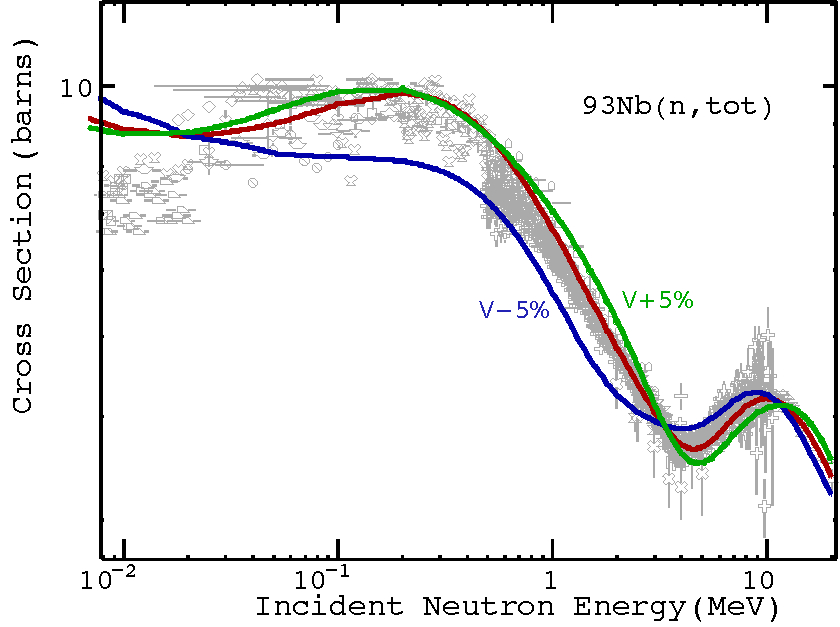
\includegraphics[width=0.7\textwidth]{figs/tot-Vv-shift}
  \caption{Effect of 5\% variation of the depth of the real optical potential on the  $^{93}$Nb(n,tot) cross section.
The baseline values are in red. }
 \label{fig:Vv-variation}
\end{figure}

Our preliminary studies indicate that the Kalman filter  adjusts the uncertainty of the fictitious model parameter, $\Delta p_{\textrm{mod}}$,  to reproduce the smallest systematic uncertainty. Thus, if the whole energy range is adequately covered by the experimental data the final result is well-defined.  In the energy ranges without measurements the result, to some extent, depends on the initial (assumed) uncertainty of the new parameter, $\Delta p_{\textrm{mod}}$. Naturally, if no experimental data are available the discussed  contribution to the uncertainty is defined by $\Delta p_{\textrm{mod}}$. In such a case,  however,  the cross section uncertainties are determined primarily by the propagation of uncertainties of the genuine model parameters, which are  much larger than the intrinsic model uncertainties.  The latter can, therefore, be neglected especially since there should be no uncertainties small enough to raise any concern. The procedure is particularly useful to simulate intrinsic uncertainties in the optical model, \textit{i.e.}, it is meant to be applied to the total cross sections. These are often very well measured which, combined with the rigid shape of the optical model predictions, results in extremely low uncertainties. There is no need to invoke such a procedure for other nuclear reaction models, {\it e.g.}, compound nucleus and preequilibrium emission, since their formulations include parameters which, to a large extent,  provide for a scaling degree of freedom.

% Practical application of the method is illustrated in Fig.~\ref{fig:fictitiousscale} for the case of  total cross section on $^{90}$Zr. At energies above 3 MeV the standard EMPIRE-KALMAN method results in uncertainties of the order of 2\%, which is smaller than the 2.8\% adopted as a systematic error of experimental data, see the upper panel.  Including the scaling degree of freedom increases predicted uncertainties in the whole energy range as shown in the lower  panel.  In particular,  at energies above 3 MeV,  the calculated uncertainties are always above the expected 2.8\%  limit, indicating that the rigidity of the model  is responsible for the suspiciously small uncertainties. Simulating intrinsic model uncertainty by introducing scaling degree of freedom is a simple and effective way of alleviating the problem. 

%A conceptually
%similar solution, correlated sampling of energy-dependent scaling parameters, has also been adopted for the MC approach in EMPIRE. In this way, the minimum uncertainty of the calculated cross-section is limited by the uncertainty of the scaling parameter which is taken as the model uncertainty.

% We note,  that scaling of the prior combined with the experimental systematic uncertainty might open the door for the Peelle's Pertinent Puzzle~\cite{Chiba:91}. The KALMAN predicted posterior cross sections may deviate from the experimental data,  as shown in the lower panel of Fig.~\ref{fig:fictitiousscale}, and  adequate measures should be taken to prevent it.

An additional source of low uncertainties has been discussed in the contribution by Leeb~\cite{Leeb-nds:2008} to  the present Workshop - neglecting correlations among numerous experiments implies statistical independence  of the respective systematic uncertainties and leads to reducing final uncertainty below individual systematic uncertainty. We refer to the original paper by Leeb for a description of an approximate method allowing one to avoid this source of underestimation. 




\chapter{Parameter fitting}



\section{Fitting Optical Model Parameters}

When the FITOMP option is selected in the input, EMPIRE will perform
automatic fitting of parameters in the direct optical model parameter
file, OMPAR.DIR (\emph{{*}-omp.dir}), and of deformation parameters in the
file containing the collective target levels, TARGET\_COLL.DAT (\emph{{*}-lev.col}).
The fitting procedure also uses the experimental data file in C4 format,
C4.dat (\emph{{*}.c4}). To ensure the existence of these files, EMPIRE should
be executed at least once before fitting begins and should be executed
with the DIRECT option selected and an incident channel optical potential
(initially) defined using the DIRPOT option, both in the initial run
and during fitting. At the moment, the FITOMP option only works for
neutron or proton scattering. 

All data relevant to an optical model fit - total, elastic and collective
inelastic cross sections and elastic and collective inelastic angular
distributions - within the requested energy range are selected from
the C4.dat file and included in the $\chi^{2}$ to be minimized. The
data points in the $\chi^{2}$ are weighted in the standard manner
using the experimental uncertainties given in the C4.dat file. Natural 
element data can be inserted in the C4.dat file and used in the fit.
In the case of neutron scattering, the file \emph{empire/RIPL/resonances/resonances0.dat}
is also searched for an s-wave strength function, which is included
in the experimental data set when found. 

The lower limit of the energy range for calculations used in a fit
is initially taken to be 1 keV while the upper limit is taken to be
30 MeV, unless modified using the FITEMX option in the input. All
relevant experimental data within this range in the C4.dat are included
in the $\chi^{2}$. The incident energies given in the input file
define the grid of energies used for calculations, unless the FITGRD
option is used. When the input file energies are used, the data points
outside of the energy interval they define are not taken into account.
That is, the fitting procedure will interpolate calculations but will
not extrapolate them. When the FITGRD option is used, the energy interval
is extended to include all data points in the initial energy range.
In both cases, the grid of incident energies is compared with those
of the experimental data and superfluous values are eliminated to
speed up the calculation. 

The parameters to be adjusted are specified by using the FITabc or
FITDEF options, described in more detail below. The RIPL parametrization
described in Refs.~\cite{RIPL2,RIPL3} is used to identify the optical
model parameters, any of which may be adjusted. The adjustable deformations
are simply those of the collective level file. Quadrupole and hexadecapole
deformations are permitted for nuclei identified as rotational, while
quadrupole and octapole dynamical deformations are permitted for those identified
as vibrational. The FITabc and FITDEF options typically identify the
desired parameter and furnish a shift in its initial value and the
maximum variation allowed during the fit with respect to its (shifted)
initial value. If no parameter adjustment is requested or all adjustable
(possibly shifted) parameters have a maximum allowed variation of
zero, the $\chi^{2}$ is calculated but no fitting is performed. At
most 20 parameters may be shifted and/or adjusted simultaneously.

At present, the optical model fitting is performed using a simple
numerical gradient search to minimize the $\chi^{2}$. The adjusted
parameters are stored in the modified OMPAR.DIR (\emph{{*}-omp.dir}) and
TARGET\_COLL.DAT (\emph{{*}-lev.col}) files. Information on the fit is written
in the FIT.OUT (\emph{{*}-ompfit.lst}) file. When a fit is complete, EMPIRE
is run one last time with all options and energies given in the input
file, excepting the fit ones. 







\section{Using Kalman filter for parameter fitting}
\label{Sec:KalmanFitting}


The multi-parameter, linearly fitting code KALMAN has proven to be very useful
in  improving evaluation procedure. Starting from an initial input, KALMAN is
able to determine an ``optimal'' set of parameters that minimizes the  overall $\chi^2$.
In order to do this, KALMAN varies the values of a given set of parameters and analyzes
the effects produced in the cross sections.  

Below, when describing filenames and instructions for the command line, the string `*' was
adopted to correspond to the main project name, that is, the root of EMPIRE's input filename
(the filename without the extension `\texttt{.inp}')

The Kalman utility within the Empire package was initially developed with the purpose of
fitting only cross sections. However, the KALMAN code itself is completely oblivious to
what quantity it is fitting since it simply receives as inputs only the experimental data
sets for which the $\chi^2$ will be minimized, the original functions before the fit, the
parameters that modify each function and their sensitivities. It is thus the role of the
auxiliary codes and of the \textit{kalman} script to manipulate the information given by
EMPIRE and write them in the appropriate format for the KALMAN code. Having this in mind,
the Kalman utility was generalized in order to be able to also fit prompt fission neutron
spectra (PFNS). Four PFNS-specific parameters were introduced into EMPIRE code: PFNTKE,
PFNALP, PFNRAT, and PFNERE (see section \ref{sec:empimp}). Each incident energy produces a
spectrum that is a function of the neutron outgoing energy. In order to accommodate
bi-dimensional fits, such as that involved with PFNS, the whole Kalman process had to be
modified. In the descriptions below the differences and similarities in format, structure
and processing between fitting cross sections and PFNS will be detailed.



We note that EMPIRE-KALMAN system is a general and powerful tool for evaluation of nuclear
reactions.  In addition to  covariance calculations it may also  be used to adjust model
parameters to reproduce experimental cross sections and other observables within the
selected reaction models and initial uncertainties of model parameters. Therefore, the
Kalman filter can be used throughout the whole evaluation procedure to ensure consistency
between cross sections, model parameters, and related covariance matrices. 


The evaluator may choose to perform a sequential  update using experimental data
for several/all  reactions or just for a single one. In the former  case, all considered
reactions are correlated and unique set of parameters along with the related covariance
matrix are produced. On the other hand, poor experimental data in one reaction channel
can negatively influence predictions for other channels. 




\subsection{Calculation of sensitivity matrices}

The sensitivity matrix file (`*\texttt{-mat.sen}' for cross sections, `*\texttt{-pfns-full-mat.sen}')
for PFNS, may be obtained through two different manners: using one of Empire's own subroutines; or using
a python script to break the calculation into smaller parts and submit them to be run
in parallel. Both methods follow the same concept and they are described in the following
subsections. Actually, the sensitivity contained in those files is not the true sensitivity,
but rather the so-called \textit{realistic sensitivity}, which is the true sensitivity
divided by the central value and multiplied by twice the interval of variation. The
reason for this is that the realistic sensitivity provides much more information regarding
the relative importance of the parameters.


\subsubsection{Sequential calculations}

By setting input parameter \texttt{KALMAN} to the value of 1 in EMPIRE's input, instead of
performing a regular run of EMPIRE calculations, it will read the sensitivity input file
in order to calculate the sensitivity matrices. This is very useful for simple fits and
when access only to a sequential machine is available. However, when fitting more than
just a few parameters, the sequential approach may take a prohibitive amount of time to
conclude the calculation. As additional limitations, EMPIRE's sensitivity routines have
not yet been prepared to generate sensitivity matrices for PFNS and for a certain class
of cross-section parameters. For these reasons, it is  advised for the user to
perform parallel calculations instead, in order to generate  sensitivity matrix files.

\subsubsection{Parallel calculations (\textit{sensitivity.py} python script)}

One may use the \textit{sensitivity.py} script, present in the `\texttt{empire/empy/qsubEmpire}'
directory, to generate sensitivity-matrix file. This method splits the full calculation
into single energy runs, submitting each incident energy for execution by a different processor node, shortening dramatically the total execution time. Firstly, it creates a directory,
named `*\texttt{\_orig/}', to where all the original input files are copied, for the calculation
of the cross sections corresponding to central values of the parameters. Afterwards, the script
reads the sensitivity input file to determine which parameters are going to be varied. Then,
for each parameter, it creates two directories with names of the form
`*\texttt{\_}\textit{keyword}\texttt{\_}\textit{I1}\texttt{\_}\textit{I2}\texttt{\_}\textit{I3}\texttt{\_}\textit{I4}\texttt{plus/}' 
and 
`*\texttt{\_}\textit{keyword}\texttt{\_}\textit{I1}\texttt{\_}\textit{I2}\texttt{\_}\textit{I3}\texttt{\_}\textit{I4}\texttt{minus/}', 
where \textit{keyword} is the parameter name, and \textit{I1}-\textit{I4} are the four parameter options.
All input files are also copied to those directories. However, in each directory, the input file
is modified by changing the value of the parameter corresponding to the directory name. If
the directory has the suffix `\texttt{plus}' then the relative increment defined in the
sensitivity input is added to the original parameter value. Likewise, for the directories
with the suffix `\texttt{minus}', then the same relative increment is subtracted from the
original parameter value. Inside each of those directories, the script \textit{qsubEmpire.py},
located in `\texttt{empy/qsubEmpire/}' directory, is called. It then splits each run into
separate directories with the same input parameters but containing only one value of
incoming energy, and finally submits each of those as different jobs to different CPU's for calculation.

The \textit{sensitivity.py} script has basically five execution options: 

\begin{itemize}

\item \textbf{-i}: Initializes the inputs and prepare to run. Executing with this option
   simply creates the  `*\texttt{\_orig/}' directory and all the parameter directories
   described above. However, \textit{qsubEmpire.py} script is not called, so the jobs are not submitted.

\item \textbf{-r}: Calls \textit{qsubEmpire.py} script to submit jobs for running. This option should
   only be executed after previous initialization (\textbf{-i})

\item \textbf{-a} or \textbf{--analyze}: After running (option \textbf{-r}), this option may be used
   to gather all the cross-section information from files `*\texttt{.xsc}' in the different directories
   that were created and calculate the sensitivity matrix, creating the sensitivity matrix file `*\texttt{-mat.sen}'.

\item \textbf{-p} or \textbf{--pfns}: After running (option \textbf{-r}), this option may be used to
   reorganize and gather all the PFNS information from files `*\texttt{-pfns.out}' in the different directories
   that were created and calculate the PFNS sensitivity matrix, creating the PFNS sensitivity matrix
   file `*\texttt{-pfns-full-mat.sen}'.

\item \textbf{-c} or \textbf{--clean}: This option is used to delete all the auxiliary directories that
   might have been created by a previous initialization or run of \textit{sensitivity.py}

\end{itemize}

If executing \textit{sensitivity.py} without specifying any options, it assumes options \texttt{-i} and,
sequentially, \texttt{-r}. There are some examples of the option usage below:

\begin{quote}
 \$EMPIREDIR/empy/qsubEmpire/sensitivity.py u235 -i \\
 \$EMPIREDIR/empy/qsubEmpire/sensitivity.py u235 -r \\
 \$EMPIREDIR/empy/qsubEmpire/sensitivity.py u235    \\
 (this is equivalent of executing, in order, both commands above) \\
 \$EMPIREDIR/empy/qsubEmpire/sensitivity.py u235 -a \\
 \$EMPIREDIR/empy/qsubEmpire/sensitivity.py u235 -c \\
\end{quote}






\subsection{Kalman script}

For KALMAN to run properly, its inputs (sensitivities, experimental data to be fitted, list of
parameters, central values for cross sections and parameters, etc.) must be found in the appropriate
files and in the expected format. Preparing those files manually for each run of KALMAN may prove to
be a cumbersome and prone-to-error task. For this reason, it is convenient to use the \textit{kalman}
script, from the `\texttt{scripts}' directory. This script connects the different ingredients needed
for the fit and organizes the results in a clear way, with the help of auxiliary codes.

The \textit{kalman} script is called in a very simple manner by providing values for a set of variables
in the command line, right after the script call. These variables are referred in the script as
\texttt{file}, \texttt{MT}, \texttt{MAT}, \texttt{EXPDAT}, \texttt{PFNS}, and \texttt{EINC}, in this
order. The first option corresponds to the project name, that is, EMPIRE's regular input file name
without the extension `\texttt{.inp}'. The second option is the MT number that should be fitted by
KALMAN. The next string corresponds to the material number (MAT) of the target. The variable \texttt{EXPDAT}
defines which experimental sets will be used in the fit, by assuming the values 0, 1, or 2.
\texttt{EXPDAT}=0 implies that all experimental data will be ignored (no fit); \texttt{EXPDAT}=1 indicates
that only experimental data for the selected MT will be considered; while \texttt{EXPDAT}=2 informs the
KALMAN code that agreement to all experimental data available in the c4 file should be considered for
fitting. At this point, it is relevant to state that, when \texttt{EXPDAT}=2, the data agreement of
the cross section (or PFNS) for a given reaction (or incident energy) may not improve, or may even get
worse after the fitting. This is due to the fact that the overall $\chi^2$ is being minimized and
worsening of agreement with data for a given reaction (or incident energy) is likely being compensated
by improvement of the agreement for all other reactions (or incident energies)
When \texttt{PFNS} has value 0 (default), KALMAN will fit only cross sections, while when
\texttt{PFNS}=1 it will fit prompt fission neutron spectra (PFNS). When \texttt{PFNS}=1, the variable
\texttt{EINC} corresponds to the incident energy for which PFNS will be fitted. The options \texttt{PFNS}
and \texttt{EINC} may be omitted when fitting cross sections since they serve only to fit PFNS. For the
time being, these fits are independent and there is no correlation between cross sections and PFNS.

Examples of valid calls of \textit{kalman} script:

\begin{quote} 
kalman pu239 18 9437 2

kalman u235 18 9228 2 1 2.53E-8
\end{quote}

In order to run properly, KALMAN needs to find a list of files in the working directory, otherwise it
will abort and print an error message. Those files are: the ENDF file (`*\texttt{.endf}'), the
sensitivity input file (`*\texttt{-inp.sen}'), the sensitivity matrix file (`*\texttt{-mat.sen}'),
and the EMPIRE's cross section file (`*\texttt{.xsc}'). If fitting PFNS instead of cross sections,
the last two files aforementioned are not necessary. However, KALMAN will then need the content of
files `*\texttt{-pfns.out}' and `*\texttt{-pfns-full-mat.sen}'.

After finishing running, the \textit{kalman} script creates several output files containing important
information regarding the fits. Such files, with a brief the description, are listed below:

\begin{itemize}

 \item `*\texttt{-out.kal}': Standard output from KALMAN. Contains information about 
   the data sets used for fitting, the $\chi^2$ obtained, the final values for the fitted parameters 
   and their corresponding uncertainties, and the correlation between parameters.

 \item `*\texttt{-expcorr.kal}': Provides the fraction of the experimental uncertainty that corresponds
   to systematical errors for each data set. This file is initially generated by the code `\texttt{genkal}',
   as file `\texttt{fort.12}', having the default value of 0.200 for all experiments.

 \item `*\texttt{-}\textit{MT}\texttt{-err.kal}', where \textit{MT} corresponds to the same script
    variable \texttt{MT} which was selected in the command line: Contains the covariances and uncertainties of the fitted curve.

 \item `*\texttt{-par.kal}': Model parameter correlations

 \item `*\texttt{-xsc.kal}': Final curves found by KALMAN for all reactions (or incident energies, in the PFNS case)

 \item `*\texttt{-cov.kal}': Contains the uncertainties (in units of \%) and correlations for all incident
    (or outgoing in the PFNS case) energies.

 \item `*\texttt{-expxsc.kal}': Contains the experimental data used in the fit.

 \item `*\texttt{-parcorr.kal}': Contains a list of the varied parameters, with their initial
     values (usually set to 1.0) and ranges of variation. Additionally, it also contains, correlation matrix for the parameters, which is usually diagonal in the first default calculation. This matrix might be changed or updated if the parameter correlation matrix is know. Then, true sensitivity matrices for each
    reaction (or each incident energy, in the PFNS case) are printed.

 \item `*\texttt{-pfns.kal}': File containing the PFNS for the fitted incident energies.

 \item `*\texttt{-}\textit{MT}\texttt{-cov.gpd}', where \textit{MT} corresponds to the same script variable
    \texttt{MT} which was selected in the command line: File to plot a three-dimensional graph of the
    covariances using \texttt{gnuplot}

 \item `*\texttt{-}\textit{MT}\texttt{-c4.gpd}', where \textit{MT} corresponds to the same script variable
    \texttt{MT} which was selected in the command line: File that contains the experimental data for the
    reaction corresponding to the \textit{MT} number used in the KALMAN fit. May be plotted together with
    `*\texttt{-}\textit{MT}\texttt{-xsc.gpd}' using `\texttt{gnuplot}'.

 \item `*\texttt{-PFNS-}\textit{INDEX}\texttt{-c4.gpd}': File that contains the pfns experimental data for
    the incident energy corresponding to the index \textit{INDEX}, as listed in file `*\texttt{-pfns.kal}'.
    May be plotted using `\texttt{gnuplot}'.

  \item `*\texttt{-}\textit{MT}\texttt{-xsc.gpd}', where \textit{MT} corresponds to the same script variable
    \texttt{MT} which was selected in the command line: Contains both the curves before and after the KALMAN
    fit. It may be plotted together with `*\texttt{-}\textit{MT}\texttt{-c4.gpd}' using \texttt{gnuplot}.

\end{itemize}

Plots of the fit can be made using the information contained in files `*\texttt{.gpd}' with the help of the
widely-available plotting tool `\texttt{gnuplot}'. Plots of the parameter correlations resulting from the KALMAN
fits can be made with `\texttt{util/kalman/corr.gp}'; correlations of the PFNS parameters with
(`\texttt{util/kalman/corr-pfns.gp}'. This plotting process is described in Section \ref{Sec:PostKalman}.

\subsubsection{Experimental Data}

For fitting either cross sections or PFNS, KALMAN needs access to the experimental data so it can calculate and
compare the $\chi^2$ at each point. The codes `\texttt{c4tokal}' and `\texttt{pnt2kal}' read experimental data
in computational format (c4 files) and write in a  way that is understandable by the KALMAN code. The former
process cross section data while the latter PFNS data.

%\subsubsection{Handling Cross-Section Experimental Data - c4tokal}
\paragraph{Handling Cross-Section Experimental Data - c4tokal.}
\label{c4tokal}

The code `\texttt{c4tokal}' reads the cross-section experimental data from the file `*\texttt{-kal.c4}',
if it exists. Otherwise, it looks for the existence of file `*\texttt{.c4}'. The reason for the additional
`*\texttt{-kal.c4}' file is that it is common, during the fitting process, that one might want to exclude
data points or even whole data sets from the fit. This way the user can edit the file `*\texttt{-kal.c4}'
while keeping the original and more complete `*\texttt{.c4}' unaltered.

EMPIRE's cross-section file `*\texttt{.xsc}' is read by `\texttt{c4tokal}' only to determine the number of
different reactions printed out by Empire and their corresponding nomenclature. In addition, the sensitivity
input file `*\texttt{-inp.sen}' is read to obtain the number of parameters to be varied in the fit.

After gathering all this information, `\texttt{c4tokal}' creates a series of output files, which will be
read by KALMAN. Below is a brief description of each of those files:

\begin{itemize}
 \item \textbf{fort.75}: contains data points, their absolute errors, and the MT number 
 \item \textbf{fort.10}: contains only the data points
 \item \textbf{fort.11}: contains only relative errors for each energy
 \item \textbf{fort.12}: contains correlations between  different experiments
 \item \textbf{KALMAN.INP}: automatically-generated input for the main KALMAN fitting code
\end{itemize}


%\subsubsection{Handling PFNS Experimental Data - pnt2kal}
\paragraph{Handling PFNS Experimental Data - pnt2kal.}

%\subsection{Experimental Data}

When compared to cross-section fiting, preparing PFNS experimental data require additional steps due to the
fact that PFNS is usually presented after normalization to Maxwellian. This normalization is often done
because PFNS vary largely across the values of outgoing energy. Since the value of the temperature used
in the Maxwellian normalization ($T_{maxw}$) is relatively arbitrary, different $T_{maxw}$ may be used
to focus on different parts of the spectra.

%\subsubsection{pnt2kal}

Instead of calling `\texttt{c4tokal}, kalman script calls the code \texttt{pnt2kal} when fitting PFNS.
This code  reads the normalized PFNS experimental data from an existing `*\texttt{.pnt}' file and
converts it to the input format needed by KALMAN. If this file does not exist,
`\texttt{pnt2kal} runs the code LSTTAB to read the PFNS data from the `*\texttt{.c4}' file and
generate the corresponding normalized `*\texttt{.pnt}' file. In this case, the code PLOTLST is initially
called to identify the index of the PFNS data in the c4 file (with output sent to file `\texttt{output.plotlst}').
Then, the Maxwellian temperature $T_{maxw}$, to which the data will be normalized, is read from EMPIRE's
PFNS output file, `*\texttt{-pfns.out}'. With that value, an input file for LSTTAB, `\texttt{input.lsttab}',
is written. The files `*\texttt{-log.plotc4}', `*\texttt{.c4}', and `*\texttt{-s.endf}', together with the
value of $T_{maxw}$, read from `*\texttt{-pfns.out}' are necessary to run LSTTAB. When LSTTAB is called
by `\texttt{pnt2kal}, its standard output is written in the file `\texttt{output.lsttab}' and the standard
pnt file `\texttt{LSTTAB.PNT}' is renamed to `*\texttt{.pnt}'.

When the `*\texttt{.pnt}' is ready, the PFNS data and all its relevant information are read at once and
stored in a structured variable. From this, the values of incident energies ($E_{inc}$) for which there
are available data are extracted. Those values are compared to the ones used for the original Empire
calculation of the PFNS, to check if PFNS were calculated at all incident energies found in the
experimental `*\texttt{.pnt}' file. If not, `\texttt{pnt2kal}' aborts since it makes no sense to fit data without
the initial calculation of its central values. In this case, an error message is printed with all the
values of $E_{inc}$ and indicating which matches could be found in the PFNS output from EMPIRE.

An important difference between integrating cross-section and PFNS fitting with EMPIRE is that, in the
former case, the initial central values are already in an easily-readable format in the file `*\texttt{.xsc}',
with the cross sections for each $E_{inc}$ in subsequent rows, and with the different reactions distributed
in columns. In the PFNS case, however, the spectra are printed as sequential blocks for the different
incident energies, with each block containing the distribution as a function of the outgoing energy. For
KALMAN to be able to fit PFNS properly, the spectra have to be rewritten in a format similar to that of
the cross sections in the file `*\texttt{.xsc}'. The code `\texttt{pnt2kal} does that by reading the
spectra from file `*\texttt{-pfns.out}' and writing them in a reformatted file, with name `*\texttt{-pfns.fmt}'.
In this new file the PFNS are written as function of the outgoing energy, with the different $E_{inc}$
distributed in columns. This way, we have the correspondence expressed in Table \ref{Tab:xsec-pfns}

\begin{table}[htb]
\begin{center}
\caption{Correspondence between cross-section and PFNS files}
\label{Tab:xsec-pfns}
\begin{tabular}{lcc}
\hline
\hline
Quantity       & cross sections  & PFNS \\
\hline
File extension & `\texttt{.xsc}' & `\texttt{-pfns.fmt}' \\
Rows           & incident energy & outgoing energy \\
Columns        & reaction        & incident energy \\
\hline
\end{tabular} 
\end{center}
\end{table}

%\textcolor{red}{ Maybe show snapshots of files .xsc, -pfns.out, and -pfns.fmt }

As mentioned, the file `*\texttt{-pfns.fmt}' contains the PFNS at all incident energies calculated
by EMPIRE. However, it is only necessary to provide to KALMAN those spectra at the same incident
energies for which there are experimental data available in the `*\texttt{.pnt}' file. For this
reason, `\texttt{pnt2kal} reads `*\texttt{-pfns.fmt}' and rewrites it in file `*\texttt{-pfns.kal}',
keeping only the columns corresponding to $E_{inc}$ found in `*\texttt{.pnt}'. This trimming process
is also done to the original PFNS sensitivity file, `*\texttt{-pfns-full-mat.sen}', with the outcome
being printed in the file `*\texttt{-pfns-mat.sen}'. For doing this, the number of parameters is
retrieved from the sensitivity input file `*\texttt{-inp.sen}'.

Finally, `\texttt{pnt2kal}' creates and writes to files `\texttt{fort.75}', `\texttt{fort.10}',
`\texttt{fort.11}', `\texttt{fort.12}', and `\texttt{KALMAN.INP}'. The contents of those files are
the same as in the case of cross-section fitting (section \ref{c4tokal}), with the corresponding
substitutions expressed in Table \ref{Tab:xsec-pfns}. In addition to those files, `\texttt{pnt2kal}'
also writes to a temporary file, named `\texttt{ENERGYANDINDEX.TMP}', that contains some information
needed later on by the \textit{kalman} script, such as number of incident energies, and index and
value of $E_{inc}$ to be fitted. This file is deleted at the end of kalman script.


\subsubsection{Central Values - genkal}

The `\texttt{genkal}' code converts the cross sections and sensitivities for all reactions into the
format needed by the KALMAN code. The cross sections are read from file `*\texttt{.xsc}' and are
rewritten in file `\texttt{fort.50}' in such a way to present the central values for the cross sections
as sequential blocks, each block corresponding to one of the reactions. The sensitivity matrices are
read from `*\texttt{-mat.sen}' and rewritten into file `\texttt{fort.52}'. The initial intervals within
each parameter may be varied by KALMAN are also written in the file `\texttt{fort.52}'. 

The central values and sensitivities in the case of PFNS fitting are converted to KALMAN format by
the same code `\texttt{genkal}' that does that for cross sections. File `\texttt{fort.50}' is
written after reading the central spectra from file `*\texttt{-pfns.kal}'. It will have the PFNS
rewritten as sequential blocks, with each block now corresponding to the spectrum distribution for
each incident energy. The PFNS sensitivity matrix will be read from file `*\texttt{-pfns-mat.sen}'
and stored again in the file `\texttt{fort.52}'. As in the cross section case, the relative intervals
for parameter variation will also be written in `\texttt{fort.52}'.

In both cross-section and PFNS cases, `\texttt{fort.52}' is renamed to `*\texttt{-parcorr.kal}' if
such file does not exist beforehand. If file `*\texttt{-parcorr.kal}' exists, then it is copied
over `\texttt{fort.52}' so, following the general EMPIRE policy,  the existing version is used rather than  the newly-generated one.
The reason for this is that, after a given run of Kalman, a user might want to edit this file in order
to modify some values, such as the range of variation for a given parameter. 

\subsubsection{KALMAN code}

If `\texttt{genkal}' and `\texttt{c4tokal}' (or `\texttt{pnt2kal}', in the PFNS case) have run
properly, then all the files needed for KALMAN to run will be ready. However, before executing
KALMAN, the \textit{kalman} script checks if the files `*\texttt{-expxsc.kal}', `*\texttt{-expcorr.kal}',
and `*\texttt{-parcorr.kal}' exist. If so, the script renames them in such a way that the fitting
code will use the existing files instead of the newly-generated ones. As mentioned above, this allows the user to
manually modify those files according to specific needs, between two consecutive runs of KALMAN.  

Afterwards, the \textit{kalman} script opens the standard KALMAN input file, \texttt{KALMAN.INP},
previously created by either `\texttt{c4tokal}' or `\texttt{pnt2kal}', using a  text editor.
At this point, the user may choose to edit this file to modify the default options before the actual
run. Once the user is satisfied with the input file, should save it and close the editor window.
This will trigger execution of the KALMAN code and start the actual fitting process.

\subsubsection{Post-KALMAN processing}
\label{Sec:PostKalman}

After the KALMAN code completed fitting the experimental data sets and has found an optimal set of parameters
that minimizes the $\chi^2$, the kalman script does a few more operations. Firstly, it
renames the output files generated by KALMAN `\texttt{fort.13}', `\texttt{fort.14}', and `\texttt{fort.15}'
into `*\texttt{-xsc.kal}', `*\texttt{-cov.kal}', and `*\texttt{-par.kal}', respectively. Secondly, it calls
the code `\texttt{kalend}' which reads the KALMAN-generated covariance and writes it in the ENDF-6 format into
file `*\texttt{-}\textit{MT}\texttt{-err.kal}'. Additionally, it also creates the files `\texttt{corrplot.d}'
and `\texttt{xscplot.d}',  for plotting.

Finally, before finishing, \textit{kalman} script uses \texttt{gnuplot} to plot the calculated covariances and
pre- and post-fit curves to compare with experimental data. To do this, it uses the \texttt{gnuplot}-instruction
file `\texttt{util/kalman/corr.gp}' (`\texttt{util/kalman/corr-pfns.gp}', in the case of fitting PFNS). Both
files `\texttt{corr.gp}' and `\texttt{corr-pfns.gp}' are set to plot the covariances directly from file
`\texttt{corrplot.d}'.  The curves before and after fitting are set to be taken from file `\texttt{xscplot.d}',
for either cross-section or PFNS calculations. Both files `\texttt{corrplot.d}' and `\texttt{xscplot.d}' are
directly generated by `\texttt{kalend}'.  The file containing the experimental data for plotting
(`*\texttt{-}\textit{MT}\texttt{-c4.gpd}' for cross sections, or when plotting PFNS, 
`*\texttt{-PFNS-}\textit{INDEX}\texttt{-c4.gpd}')
was previously generated either by `\texttt{c4tokal}' (in the case of cross sections) or by
`\texttt{pnt2kal}' (in the PFNS case). However, both `\texttt{corr.gp}' and `\texttt{corr-pfns.gp}' are set
to take the experimental data from file `\texttt{expxscplot.d}'. Therefore, right before calling
`\texttt{gnuplot}', \textit{kalman} script copies file `*\texttt{-}\textit{MT}\texttt{-c4.gpd}'
(or `*\texttt{-PFNS-}\textit{INDEX}\texttt{-c4.gpd}', depending to which quantity has been fitted) to
file `\texttt{expxscplot.d}'. 

Once the `\texttt{gnuplot}' command is executed, the three-dimensional graph of the covariance should be
plotted. Figure \ref{Fig:CorrU235} shows examples of such graphs for the case of fission (top pannel)
and capture (bottom pannel) of neutrons inciding on $^{235}$U. 
\begin{figure}[htb]
 \begin{center}
  \vspace{-0.0cm}
  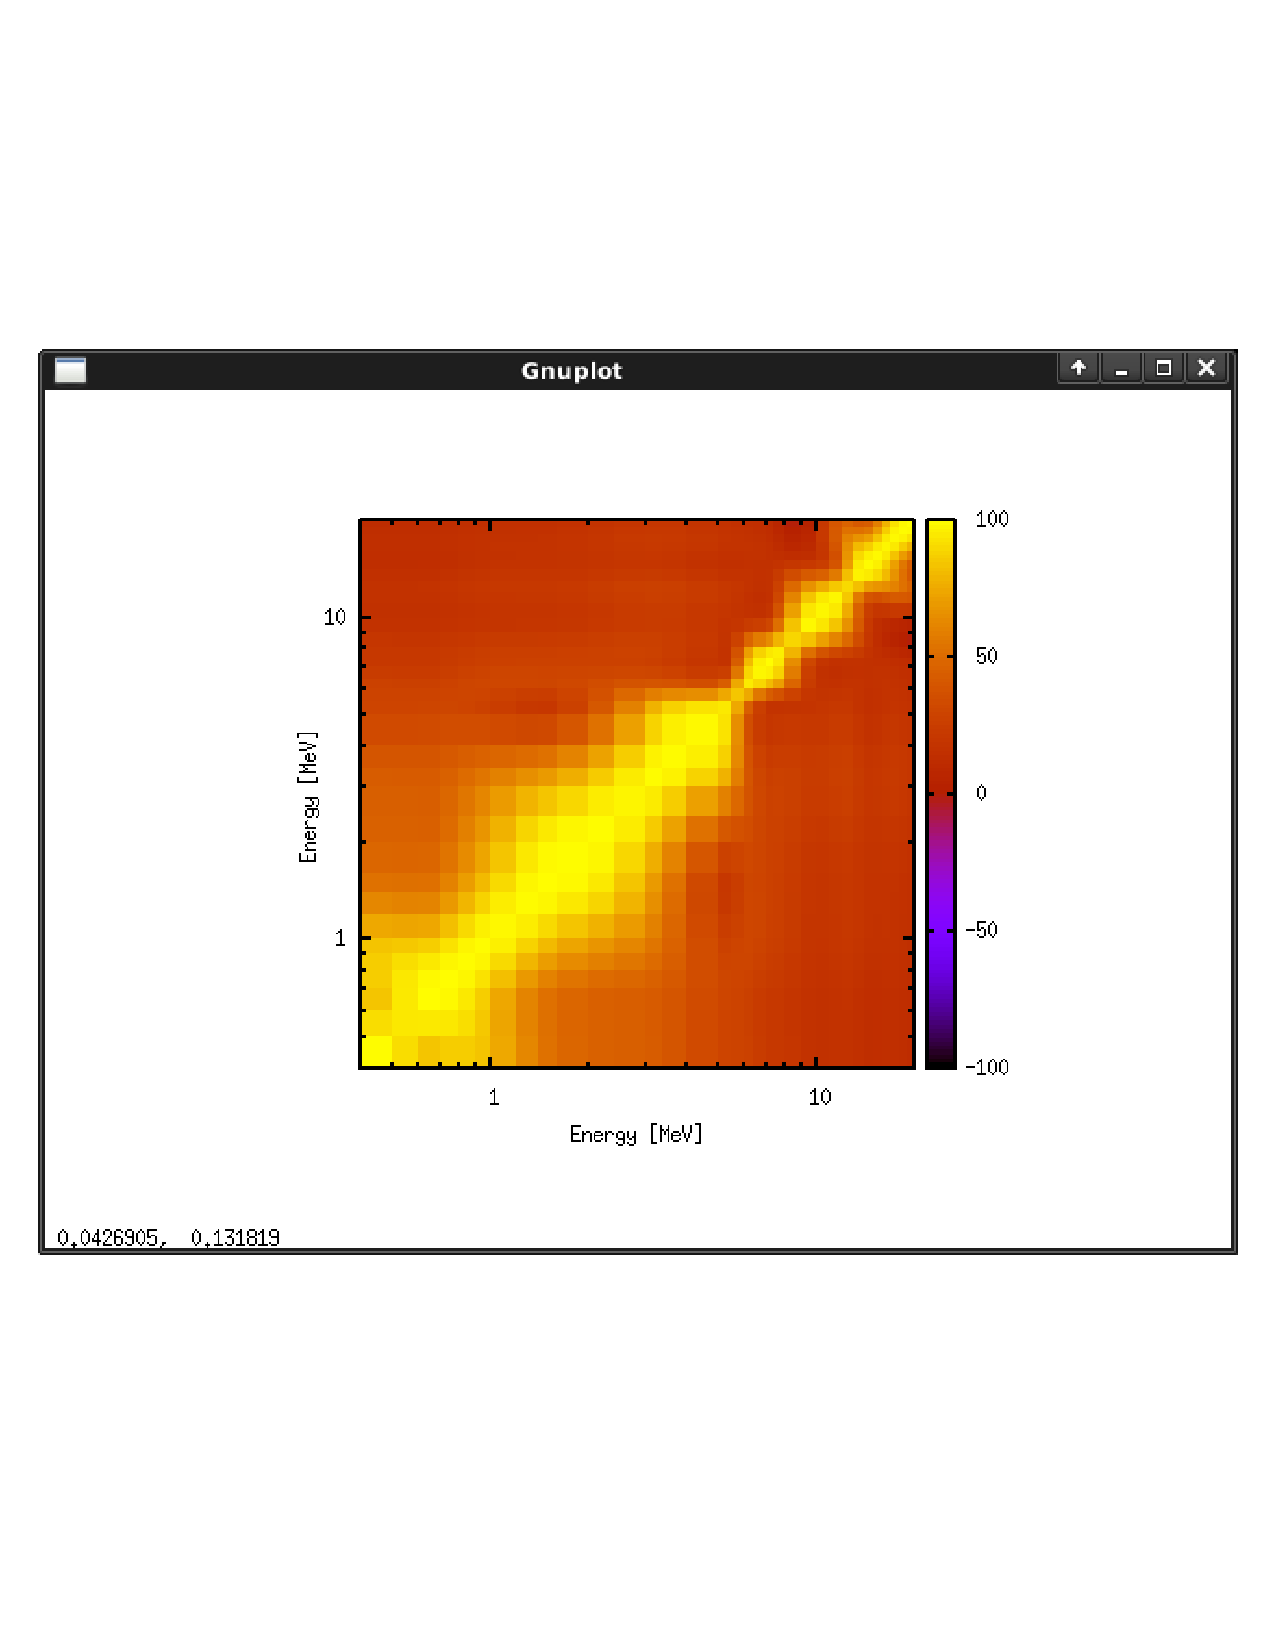
\includegraphics[trim = 5mm 60mm 5mm 50mm, clip,width=4.8in,angle=0.0]{figs/u235-fission-correlation-plot} \\
  \vspace{-3.0cm}
  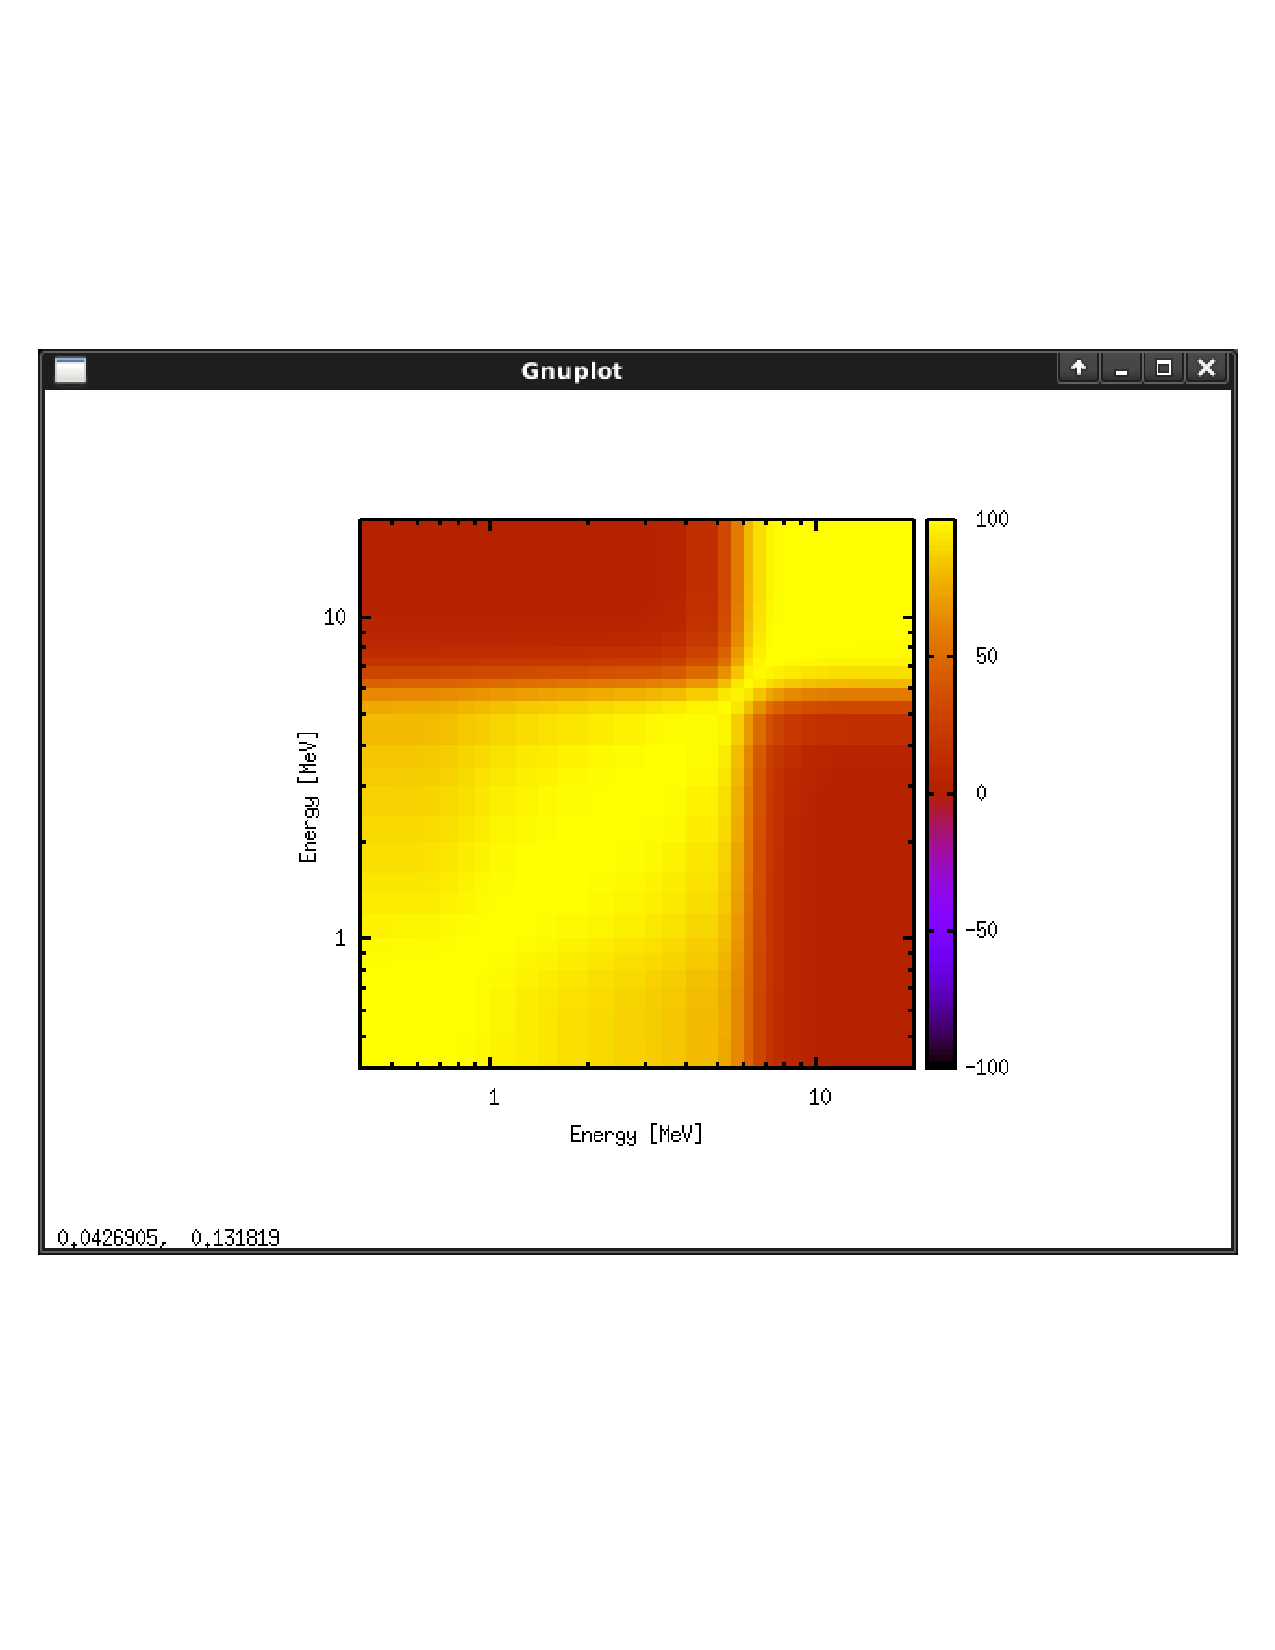
\includegraphics[trim = 0mm -8mm 0mm 0mm, clip,width=5.0in,angle=0.0]{figs/u235-capture-correlation-plot} \\
 \end{center}
 \vspace{-4.5cm}
 \caption{Correlation matrices for neutron-induced fission (top) and capture (bottom) reactions
   ($MT=18$ and $102$, respectively) for material $^{235}$U.}
 \label{Fig:CorrU235}
\end{figure}
After the user closes the covariance-graph window and hits enter on the terminal, the graph of prior- and
post-KALMAN fitting curves is plotted. Figure \ref{Fig:PriorPostU235} shows the agreements with fission
(top pannel) and capture (bottom pannel) experimental data of the calculated cross sections before
(blue curve) and after (green curve) the fit. 
\begin{figure}[htb]
 \begin{center}
  \vspace{-0.0cm}
  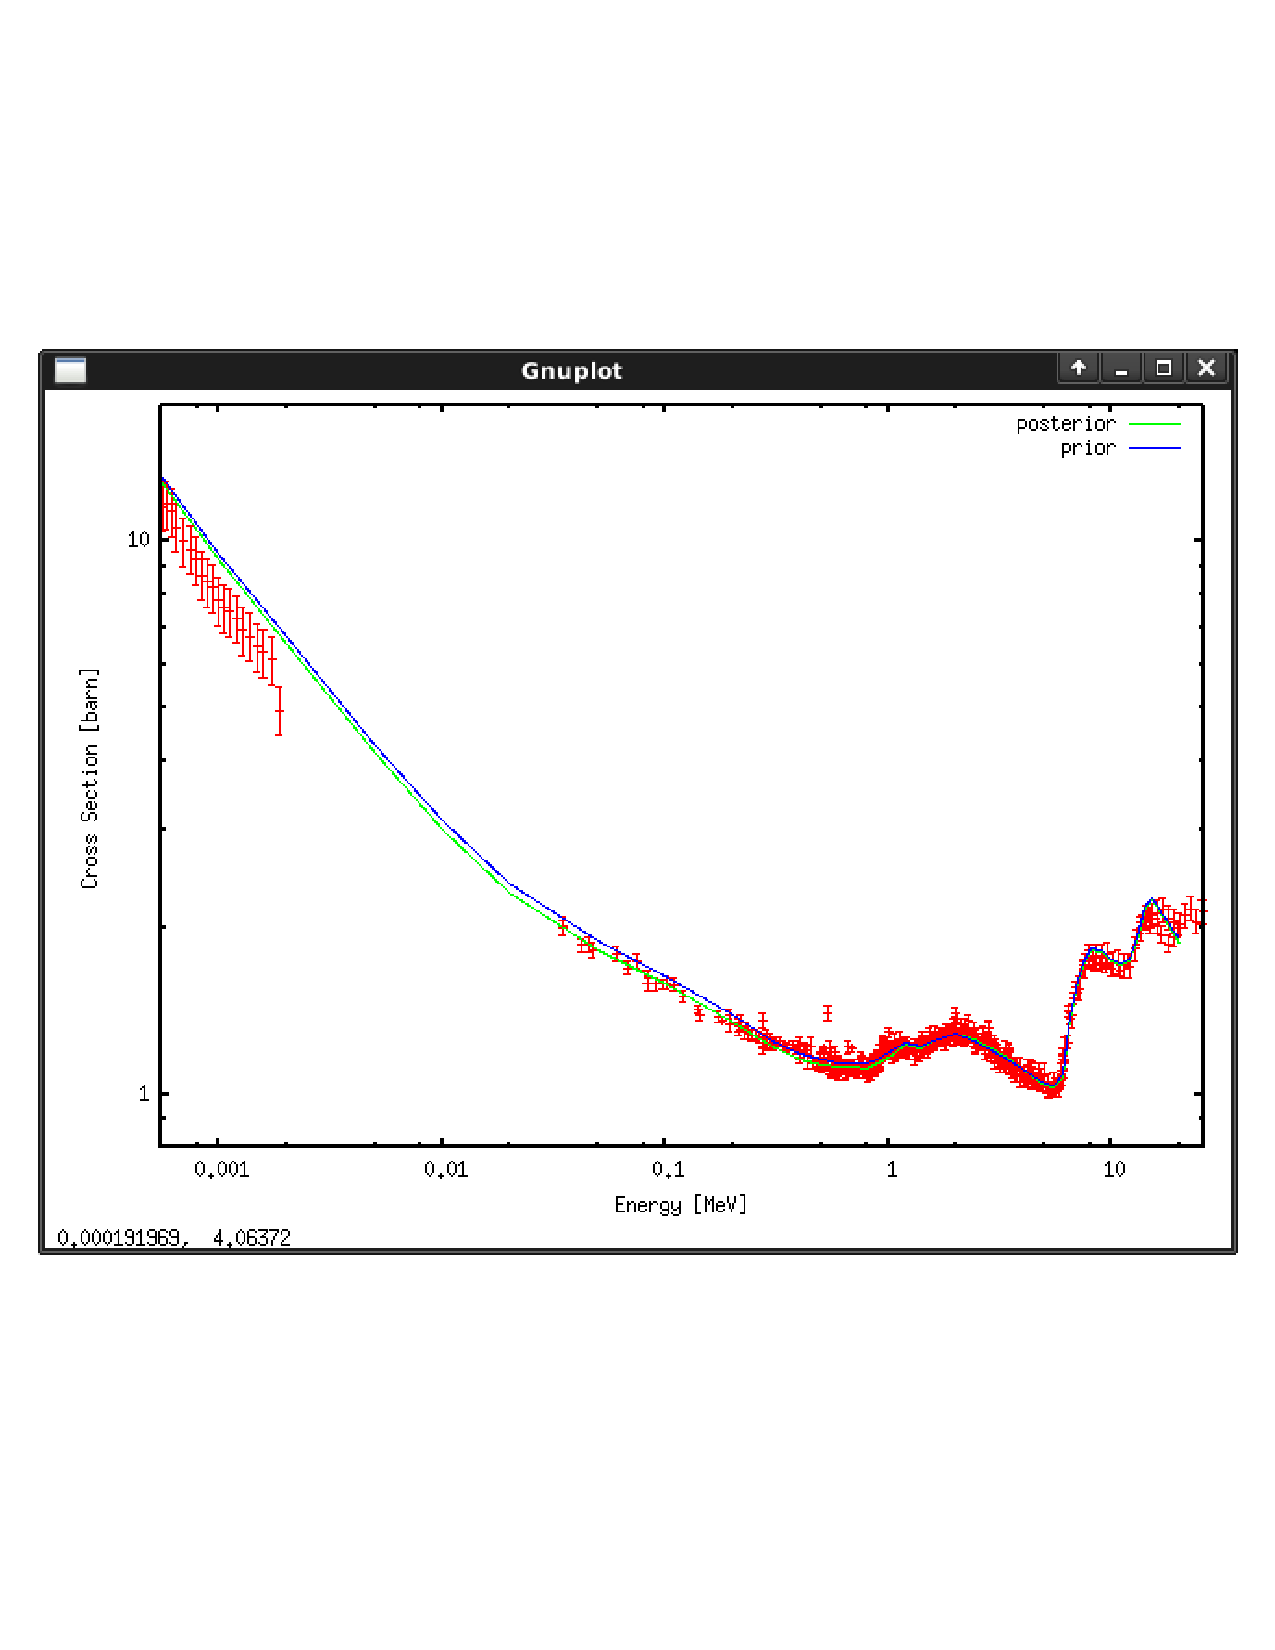
\includegraphics[trim = 5mm 60mm 5mm 50mm, clip,width=4.7in,angle=0.0]{figs/u235-fission-prior-post} \\
  \vspace{-3.0cm}
  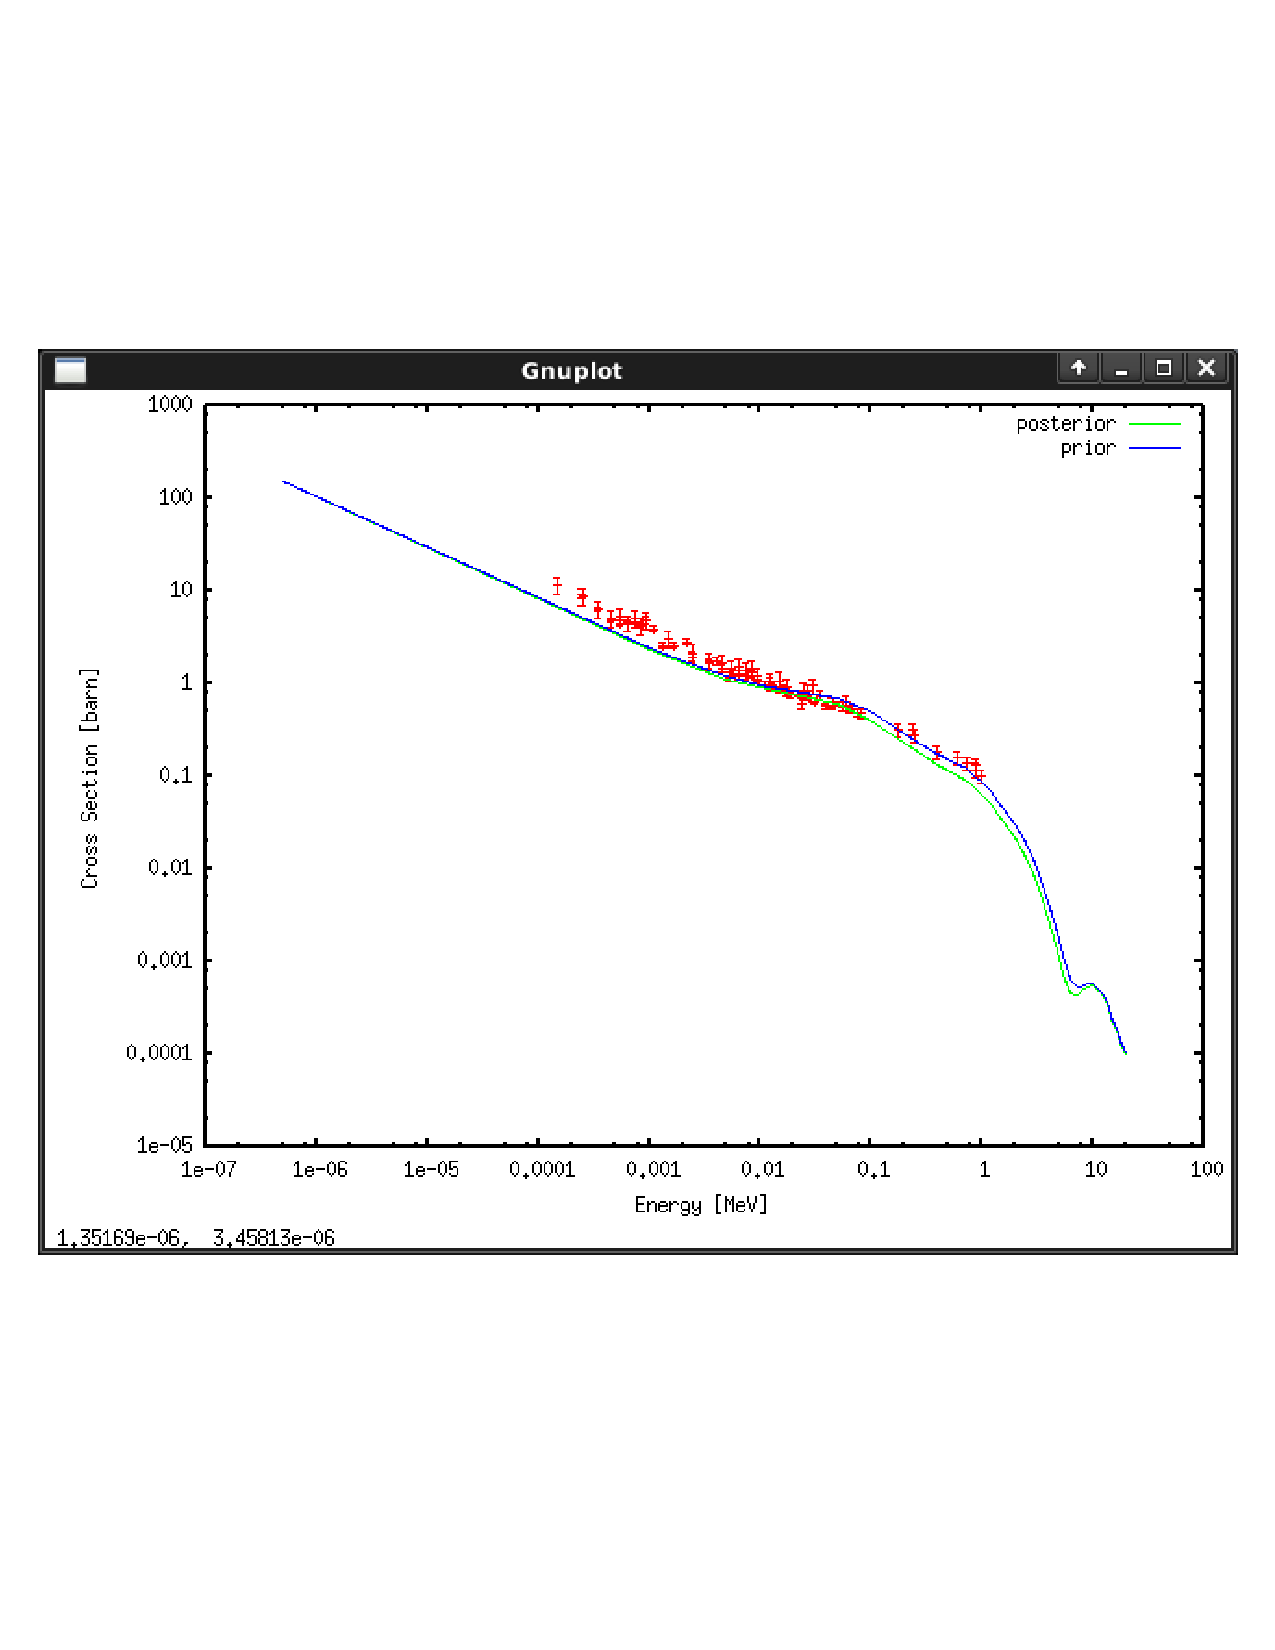
\includegraphics[trim = 0mm -8mm 0mm 0mm, clip,width=4.9in,angle=0.0]{figs/u235-capture-prior-post} \\
 \end{center}
 \vspace{-4.5cm}
 \caption{Cross section for the neutron-induced fission (top) and capture (bottom) reactions 
($MT=18$ and $102$, respectively) for material $^{235}$U, comparing the agreement with experimental
data between the curves prior and post KALMAN fitting.}
 \label{Fig:PriorPostU235}
\end{figure}

It is important to mention that this post-fitting calculation does not necessarily correspond to
the exact  result that one should get when the new values of the parameters are put back into
EMPIRE's input file for a new run of EMPIRE. This happens because the Kalman filter is a linear
fitting code, which means that, the effect of perturbing a given parameter will be calculated by 
linearly interpolating (or extrapolating) the sensitivity matrix. Hence the importance of choosing wisely the intervals
of variation, both when obtaining the sensitivity matrix and when editing `*\texttt{-parcorr.kal}'
to avoid falling out of the linearity regime. The final effect of fitting parameters through KALMAN
will thus only be known after the new parameter values are put back into EMPIRE's input file and new
cross sections or PFNS are calculated.

\subsection{Fitting example: \texorpdfstring{$^{235}$U}{235U}}


As an example, we present below the entire process of generating the central values, sensitivities,
and KALMAN fits, with a complete set of commands, for the target material $^{235}$U.

Once EMPIRE's initial input files have been defined and assuming EMPIRE's main input file is named
as `\texttt{u235.inp}', one can run EMPIRE, generate ENDF-6 formatted file, and process it for
plotting by issuing the following commands:
\begin{quote}
 \$EMPIREDIR/scripts/runE u235 \\
 \$EMPIREDIR/scripts/format u235 9228 \\
 \$EMPIREDIR/scripts/process u235 
\end{quote}
or, alternatively:
\begin{quote}
 \$EMPIREDIR/scripts/run u235 9228
\end{quote}

In order to calculate sensitivities, the sensitivity input file `\texttt{u235-inp.sen}' must be created,
containing the list of parameters to be varied. This file may contain both cross-section and PFNS
parameters. Since, at the time being, those fits are independent and uncorrelated, the cross-section
sensitivity file (`\texttt{u235-mat.sen}') will contain zero sensitivities for the PFNS parameters and,
likewise, the PFNS sensitivity file (`\texttt{u235-pfns-full-mat.sen}') will contain vanishing
sensitivities for the cross-section parameters. To calculate the sensitivities and generate the
sensitivity matrix files for both cross sections and PFNS one may use the commands:

\begin{quote}
  \$EMPIREDIR/empy/qsubEmpire/sensitivity.py u235    \\
  \$EMPIREDIR/empy/qsubEmpire/sensitivity.py u235 -a \\
  \$EMPIREDIR/empy/qsubEmpire/sensitivity.py u235 -p \\
\end{quote}

At this stage, all the files needed to start the fitting process have been generated. If the user
chooses to fit cross sections taking into consideration experimental data for all reactions available
in the \texttt{c4} file (`\texttt{u235.c4}'), and wishes to see the correlation and prior/post-fit
graphs for fission reaction, for example, he/she may use the command:

\begin{quote}
kalman u235 18 9228 2
\end{quote}
The result of this KALMAN run is shown in Figures \ref{Fig:CorrU235} and \ref{Fig:PriorPostU235},
top pannels. If, however, the user chooses instead to see the KALMAN predictions for capture,
the following command may be used:

\begin{quote}
kalman u235 102
\end{quote}
Figures \ref{Fig:CorrU235} and \ref{Fig:PriorPostU235}, bottom panels, show the results of this run.

To fit PFNS experimental data for all incident energies contained in the \texttt{c4} file
(`\texttt{u235.c4}'), but to plot the KALMAN predictions for thermal energy, one may use the command:

\begin{quote}
kalman u235 18 9228 2 1 2.53E-8 
\end{quote}

After the final parameters, which may be found in this case in file `\texttt{u235-out.kal}', are
put back into EMPIRE's main input file, `\texttt{u235.inp}, EMPIRE may be executed again with command:
\begin{quote}
 \$EMPIREDIR/scripts/run u235 9228
\end{quote}
to obtain the final results, for cross sections and PFNS, after the KALMAN fit
Figures \ref{Fig:U235-fission}, \ref{Fig:U235-capture}, and \ref{Fig:U235-pfns} show examples of
results for cross-section and PFNS fits for $^{235}$U using Kalman filter integrated with EMPIRE.


\begin{figure}[htb]
 \begin{center}
  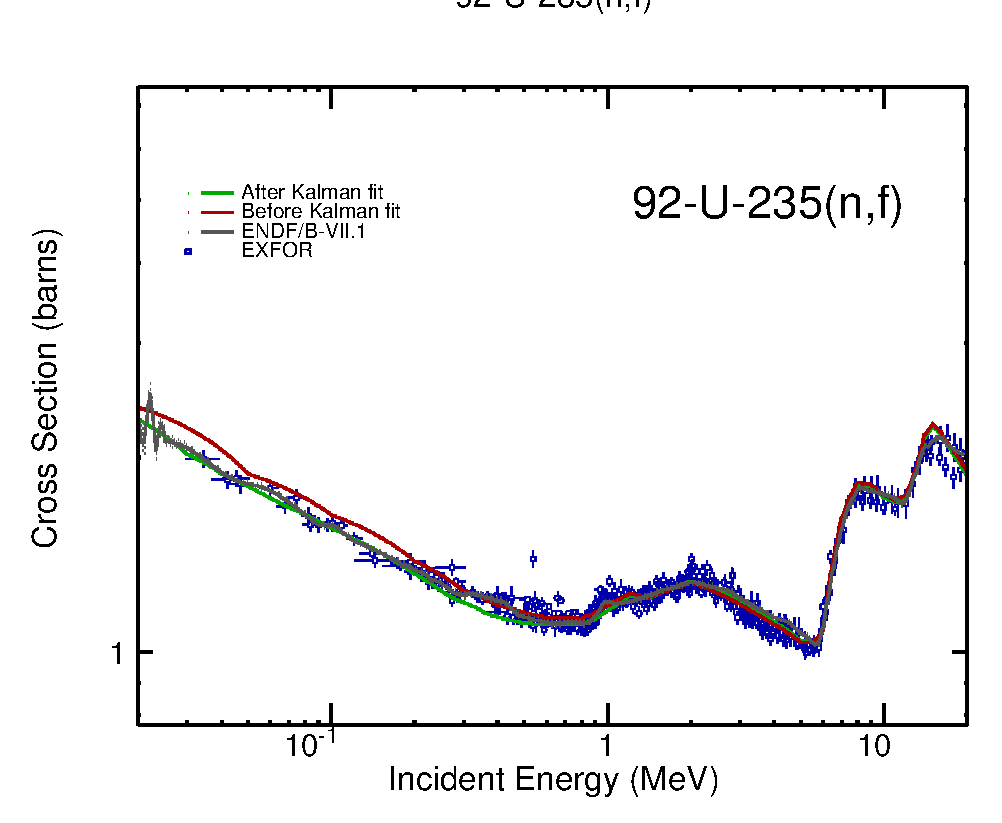
\includegraphics[trim = 5mm 4mm 5mm 14mm, clip,width=\textwidth,angle=0.0]{figs/u235-fission} 
 \end{center}
 \vspace{-4mm}
 \caption{Comparison between fission cross sections calculated by EMPIRE using input parameters
  obtained before and after fitting using Kalman filter. Evaluation from ENDF/B-VII.1 library and
  experimental data from EXFOR are also plotted.}
 \label{Fig:U235-fission}
\end{figure}

\begin{figure}[htb]
 \begin{center}
  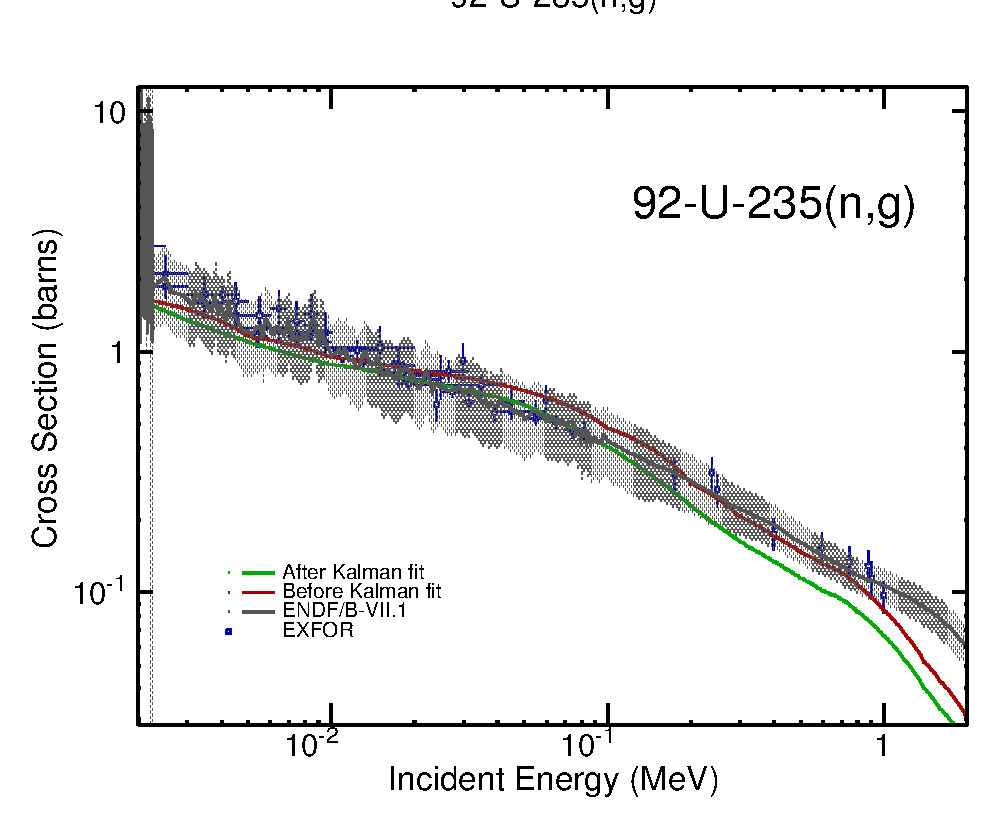
\includegraphics[trim = 5mm 4mm 5mm 14mm, clip,width=\textwidth,angle=0.0]{figs/u235-capture} 
 \end{center}
 \vspace{-4mm}
 \caption{Comparison between capture cross sections calculated by EMPIRE using input
  parameters obtained before and after fitting using Kalman filter. Evaluation from
  ENDF/B-VII.1 library and experimental data from EXFOR are also plotted. Even though
  the agreement of the post-fit curve seems worse than that of the pre-fit one, this is
  compensated by improvements at other reactions, minimizing the overall $\chi^2$. This
  may happen when the option to fit data for all reactions is selected.}
 \label{Fig:U235-capture}
\end{figure}

\begin{figure}[htb]
 \begin{center}
  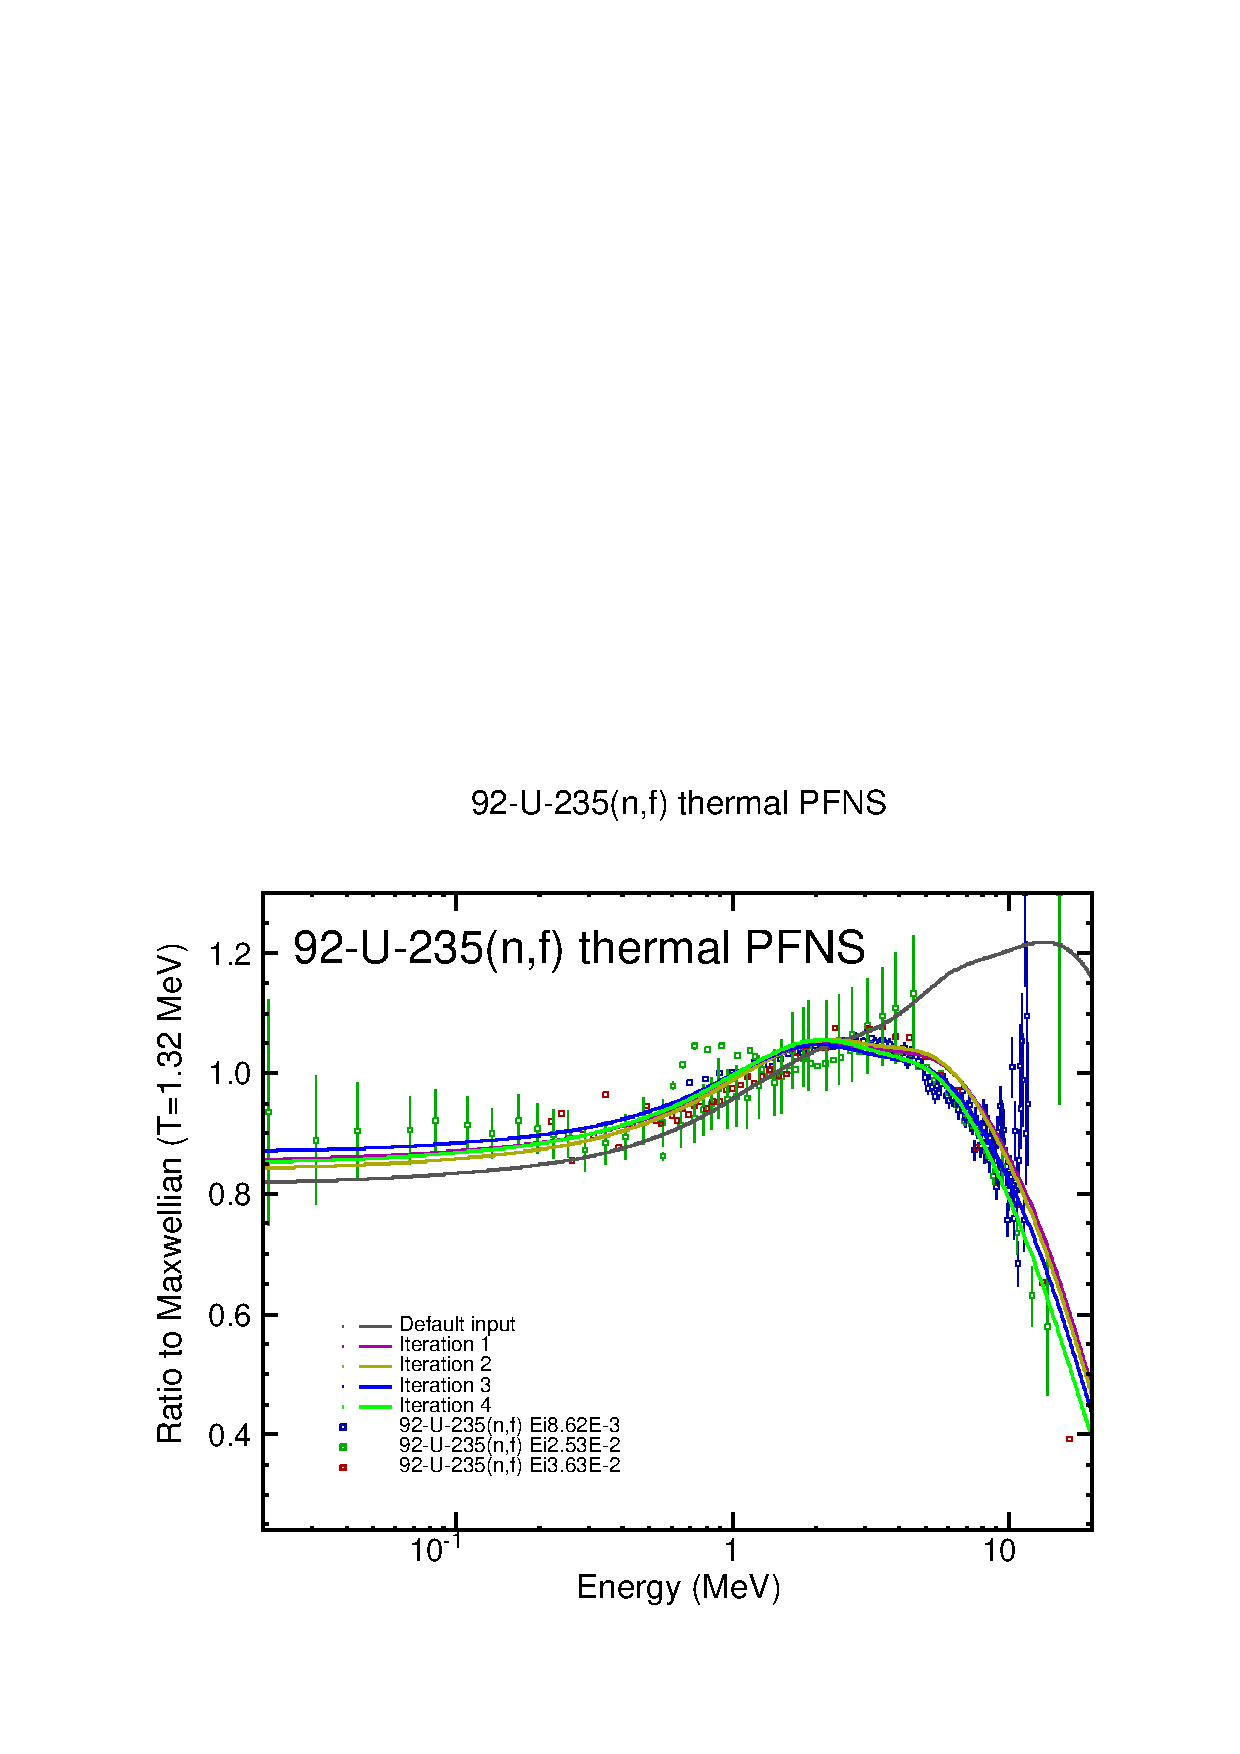
\includegraphics[trim = 4mm 4mm 4mm 5mm, clip,width=\textwidth,angle=-0.0]{figs/u235-pfns-LosAlamos} 
 \end{center}
 \vspace{-4mm}
 \caption{Prompt fission neutron spectra (PFNS) for thermal neutrons calculated by EMPIRE
  using a default input and input files containing PFNS parameters after different numbers
  of KALMAN-EMPIRE iterations. For iterations 3 and 4, additionally to iterating a new sequence
  of KALMAN and EMPIRE runs, some spurious data points were removed from the fitting process.}
 \label{Fig:U235-pfns}
\end{figure}




\newcommand{\mub}{$\bar{\mu}$}
\newcommand{\nub}{$\bar{\nu}$}
\section{Fitting \texorpdfstring{\mub\ and \nub}{Mubar and Nubar} in Empire with Kalman}
%\section{Fitting Mubar and Nubar in Empire with Kalman}

The fitting code KALMAN, used within the EMPIRE nuclear modeling system, is a fitting package based on the
Kalman fitting technique where a set of empire model parameters are adjusted to fit a set
of data \cite{KALMAN}. The required input is
only the data (observables) being fit, the predicted value for those data from the model, and the ``sensitivity''
of each observable to each fitted parameter, where the ``sensitivity'' is simply the first derviative of the
observable with respect to the fitted parameter. These sensitivities are calculated numerically. They
are prepared as a matrix, where one dimension is the parameter index and the other is the index of the observable.
For each parameter $x_{i}$, the sensitivity of observable $OB(j)$ is calculated by adjusting the parameter
up and down by a given amount, and then calculating the observables for these adjusted
parameters, which are designated with a superscript $+$ or $-$. The resulting sensitivity of the $jth$ observable to
the $ith$ parameter is then simply given by

\begin{equation}
\label{Eq:sens}
{\rm Sens}(j)_{i} = (OB(j)^{+} - OB(j)^{-})/(x_{i}^{+} - x_{i}^{-})
\end{equation}

This matrix of sensitivities, along with the predicted values of the observables without adjustment (often
referred to as the ``central values,'' as the parameters are set to original values between the ``+'' and ``-''
values, hence ``central'') are then used to adjust the parameters using the Kalman method to minimize the
difference between the fitted value and the prepared set of observables in the standard C4 data format,
using the usual definition of $\chi^{2}$ as the sum of differences between the model predictions $Y_{i}$
and measured quantities $y_{i}$ divided by the measurement uncertainty $\sigma_{i}$. The sum of the
squares of these ratios forms
$\chi^{2}$,
\begin{equation}
\label{eqn_chi2}
\chi^{2} = \sum_{i=1}^{n}((Y_{i} - y_{i})/\sigma_{i})^{2}
\end{equation}
where the summation is over all measured observables $n$. For further details about
the Kalman approximation used in fitting see \cite{KALMAN}.

This approach has been successfully used with the Empire package for fitting cross sections. It
includes, but is not limited to, total, elastic, inelastic, (n,2n), fission, and capture. The user
creates a file which lists each empire parameter to be fitted along with a displacement
which limits the range of the parameter when fitted by the Kalman code and also to determine
the ``+'' and ``-'' values of Eq.~\ref{Eq:sens} when calculating the
sensitivity to the parameters for each fitted cross section. As such, these values should be
chosen to be as large as possible as not to restrict the fit, but also not so large as to
introduce nonlinearities into the calculation of the sensitivities. This amount varies for each
parameter and its functional form within the EMPIRE code.

Here we discuss an extension of this fitting that will allow one to fit in addition to the
usual cross sections, the prompt neutron fission spectra (PFNS), the average cosine of the
scattering angle for elastic neutron scattering (\mub), and the average number of neutrons
produced in fission (\nub). For a detailed description of the PFNS fitting, see
section~\ref{Sec:KalmanFitting}. The addition of \mub\ and \nub\ fitting in empire/kalman is described here.

\subsection{\texorpdfstring{\mub}{Mubar} (Mubar)}

When fitting EMPIRE calculations to experimental observables with Kalman, the data are prepared
for the fitting code by the kalman script which controls the processing of
the C4 data and the standard EMPIRE cross sections and sensitivities into the format used by the
KALMAN code. A mapping function is used to map each reaction from EMPIRE to the corresponding
MT as specified for that reaction in the C4 data file. 
This is done for various MF3 cross sections, but not for angular distributions, etc. As a first
step toward including sensitivity to the angular distributions we describe the addition of the
capability of fitting the \mub\ as calculated by EMPIRE to experimental values. This involves 2
steps: (i) fitting of the experimental elastic angular distributions to produce an experimental
value for \mub\ with uncertainties and (ii) the addition of \mub\ as another ``reaction'' in the
file of cross sections produced by EMPIRE for fitting with Kalman (the XSC file). Here we
describe the preparation of both the experimental and calculated values.

The experimental differential cross sections (C4 MF4/MT2) for elastic scattering are fit
with a Legendre polynomial expansion to extract the coefficient from the fit for the first
Legendre coefficient, which corresponds to \mub\ or the average scatting cosine (here, the
0th Legendre parameter corresponds to the elastic scattering cross section). To fit these
Legendre coefficients two similar approaches have been developed.

In the first approach, ang\_mu.f code, developed by A. Trkov at BNL, scans the input C4 data file
and each section of elastic scattering
differential cross sections are fitted using standard least-squares with the
sum of the squares of the differences between the experimental cross sections
and the Legendre fit being minimized. This method will iterate the fit, automatically increasing
the order of the fit until the maximum relative difference between the data and the fit are
less than the maximum relative error in the diff. cross section divided by $\sqrt{2}$, but never
less than 7\%.  The
order of the fit is also never allowed to exceed $l=22$ or 2/3 the number of points in the angular
distribution, whichever is smaller. This will produce a value for \mub\ for each elastic
differential cross section encountered in the C4 file from the $0^{th}$ and $1^{st}$ Legendre
moments as
\begin{equation}
\label{Eq:mubar}
\bar{\mu} = \frac{c_{1}}{3 c_{0}}
\end{equation}
where the factor of 3 comes from re-normalizing the angular distribution by $2l+1$, with $l=1$.
These fitted Legendre coefficients are written to the C4 file with MF154/MT2 which are paired
with the calculated values for \mub\ from Empire, which are assigned to MF3/MT251. The files
are processed and prepared for the Kalman fitting code by the routine c4tokal.f90.

\begin{figure}[htb]
 \begin{center}
  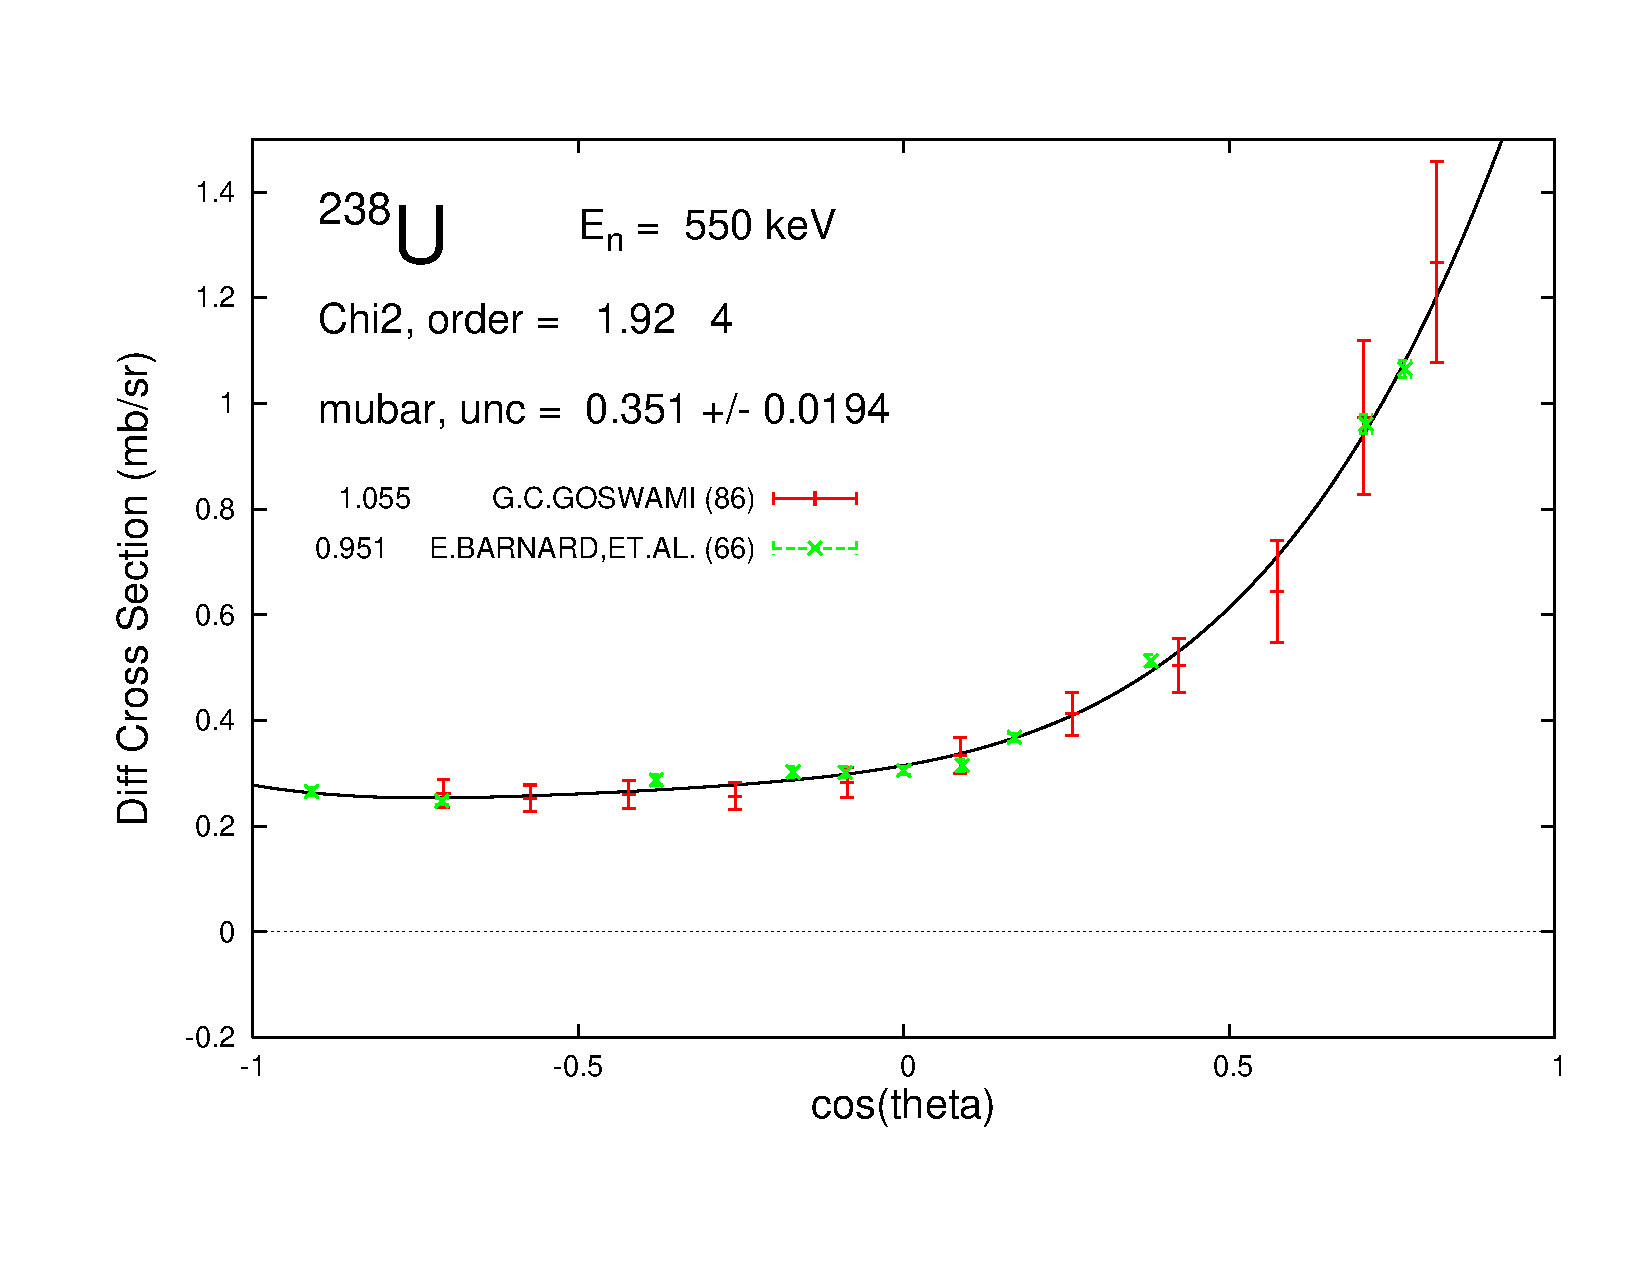
\includegraphics[trim = 15mm 15mm 0mm 0mm, clip,width=5.0in,angle=0.0]{figs/mubar} \\
 \end{center}
 \vspace{-4mm}
 \caption{Legendre fit to differential cross section data at $\rm{E} = 550$ keV. There were 2 data sets
 available at this energy. Each data set was adjusted by a scale factor that was fitted along
 with the Legendre coefficients by including a penalty term in the $\chi^{2}$ (see Eq.~\ref{Eq:sclchi}).
This resulted in a good fit to the data with only a 4th order Legendre fit with a final reduced $\chi^{2}$ of 1.92.}
 \label{Fig:mufit}
\end{figure}

The Legendre fitting of the angular distributions will suffer if the number of data points
is small or the data do not cover enough angular range to successfully constrain the fit. In an attempt
to increase the coverage, when available, a second version of the Legendre fitting was
developed that will group the data by incident neutron energy, which then may fit more than
one C4 data section at once, increasing the number of points and angular coverage which
may result in a better fit. In this version, the uncertainty of the individual data
points are used in creating the $\chi^{2}$, as in Eq. \ref{eqn_chi2}. Each data set
is assigned a systematic uncertainty and a scale factor is used to
bring the various data sets into agreement, which is important to achieve a
good fit when fitting more than one data set at a time.
A scale factor $f$ for each data set is added to the definition of $\chi^{2}$ and
a penalty term added for each data set weighted set's systematic error $\sigma_{f}$ 
as shown in Eq.~\ref{Eq:sclchi} (see ref. \cite{Agostini:94}).
\begin{equation}
\label{Eq:sclchi}
\chi^{2} = \sum_{i=1}^{n}((Y_{i} - fy_{i})/f\sigma_{i})^{2} + ((f-1)/\sigma_{f})^{2}
\end{equation}
The order of the Legendre fit was also automatically increased, where the order of the
fit would increase until $\chi^{2} < 2.5$ but never allowed to exceed 2/3 of the total number
of points being fit. This method yielded uncertainties on the coefficients
of the Legendre polynomials which could then be directly propagated to an uncertainty in \mub\ 
as defined in Eq.~\ref{Eq:mubar}. An example of this fitting procedure is shown in Figure~\ref{Fig:mufit}.
Here 2 different data sets were each assigned a 5\% systematic error. The fit scaled the data set of
Goswami, et. al. up by 5.5\% and the data set by E.Barnard, et. al., down approximately 5\%. The
resulting angular distribution was fit using only a $4^{th}$ order Legendre polynomial
with a reduced $\chi^{2}$ of 1.92. 

\begin{figure}[htb]
 \begin{center}
  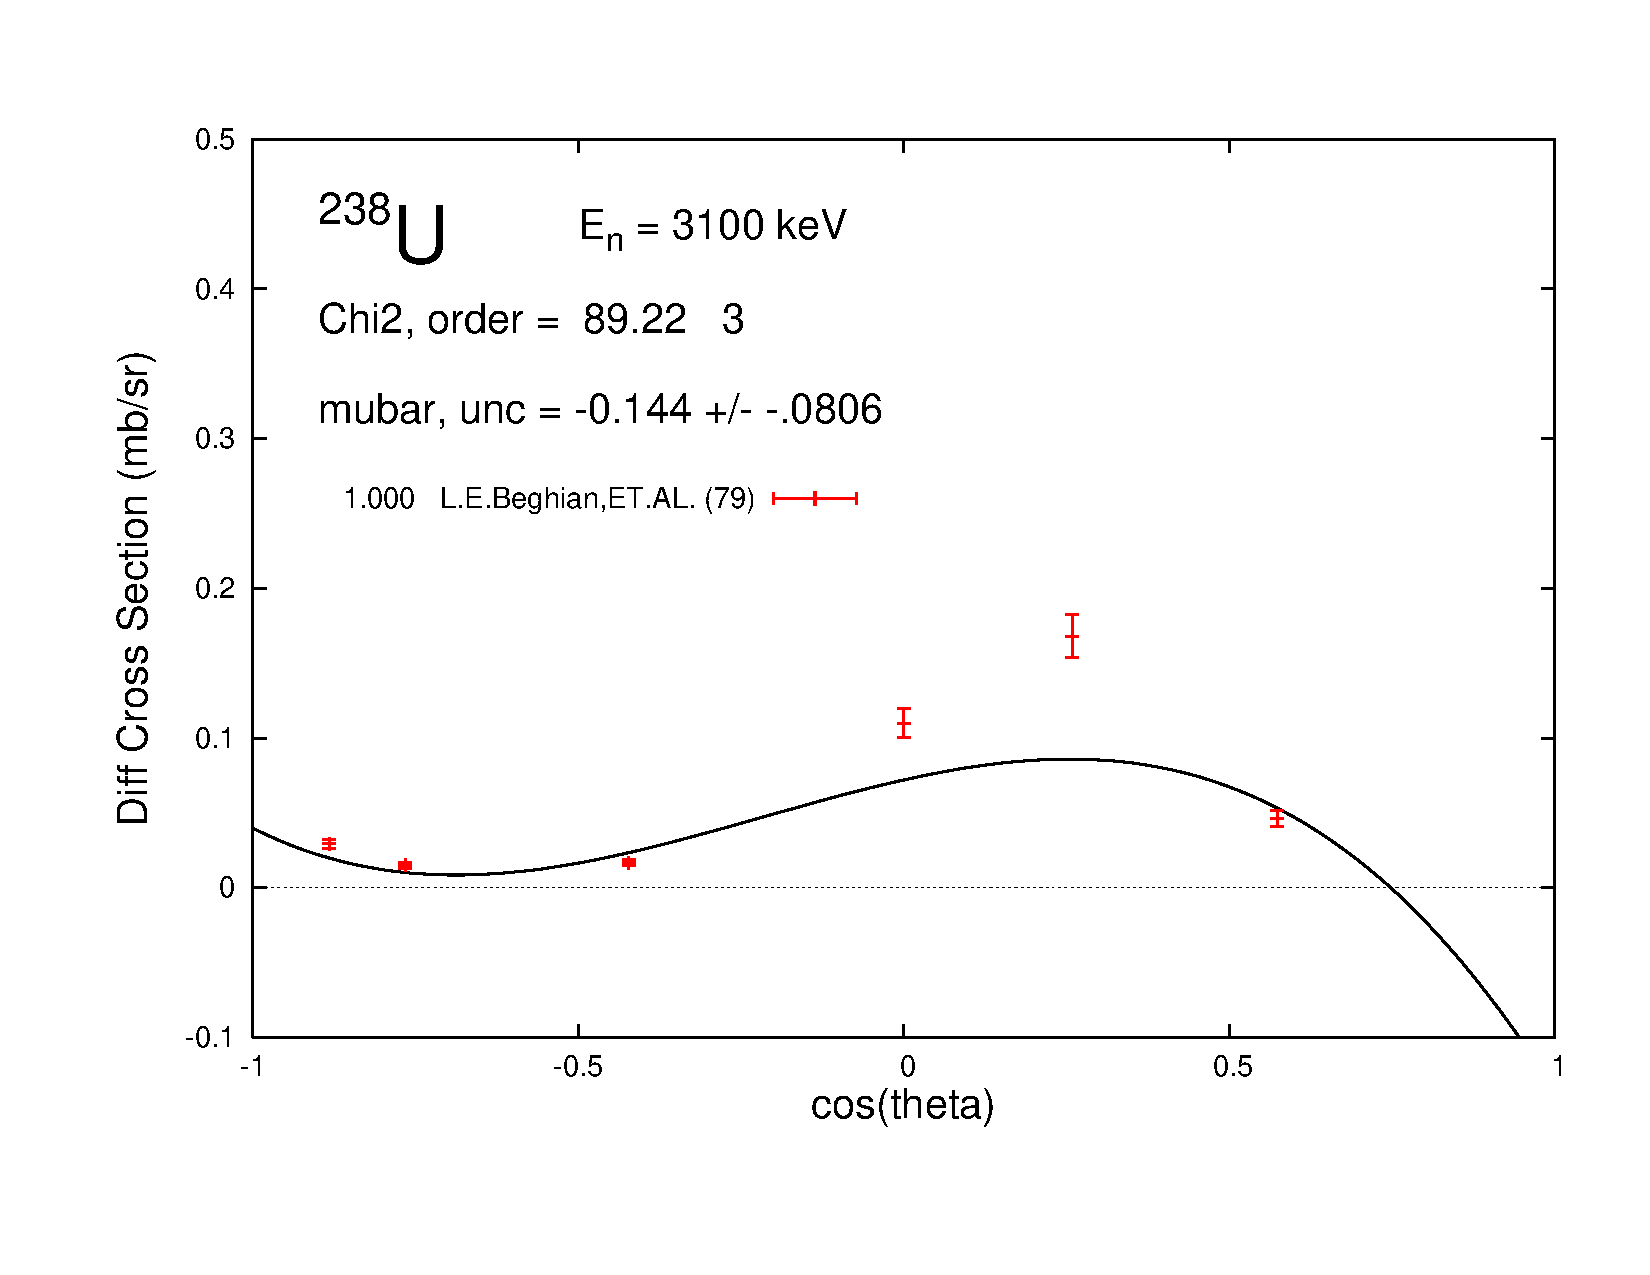
\includegraphics[trim = 15mm 15mm 0mm 0mm, clip,width=5.0in,angle=0.0]{figs/bad_mubar} \\
 \end{center}
 \vspace{-4mm}
 \caption{Legendre fit to differential cross section data at $E = 3.1 MeV$. An example of
 a data set with too few points and too small angular coverage. The fit fails with negative
 cross sections being produced, resulting in a nonsensical value for \mub.}
 \label{Fig:badmu}
\end{figure}

These procedures for fitting \mub\ are fairly automated, but care must be taken and each fit must
be visually checked. A common cause for a bad fit is simply insufficient
angular coverage or too few points to constrain the fit, or both. An example of this type of failure
is shown in Fig.~\ref{Fig:badmu}. Here, there are few data points and none at forward angles. The
resulting fit has a negative cross section at forward angles. The resulting value for \mub\ is meaningless
should not be used. 

Another case where there are often problems are at high energy ($\rm{E}_{n} > 10$ MeV), where the
angular distribution is very forward peaked. Fitting these distributions usually requires a very
high order Legendre polynomial, which can easily become unconstrained at very forward or backward angles,
resulting in a bad value for \mub. An example of such a fit at $E_{n} = 15$~MeV is shown in
Fig.~\ref{Fig:bad_high}.
\begin{figure}[htb]
 \begin{center}
  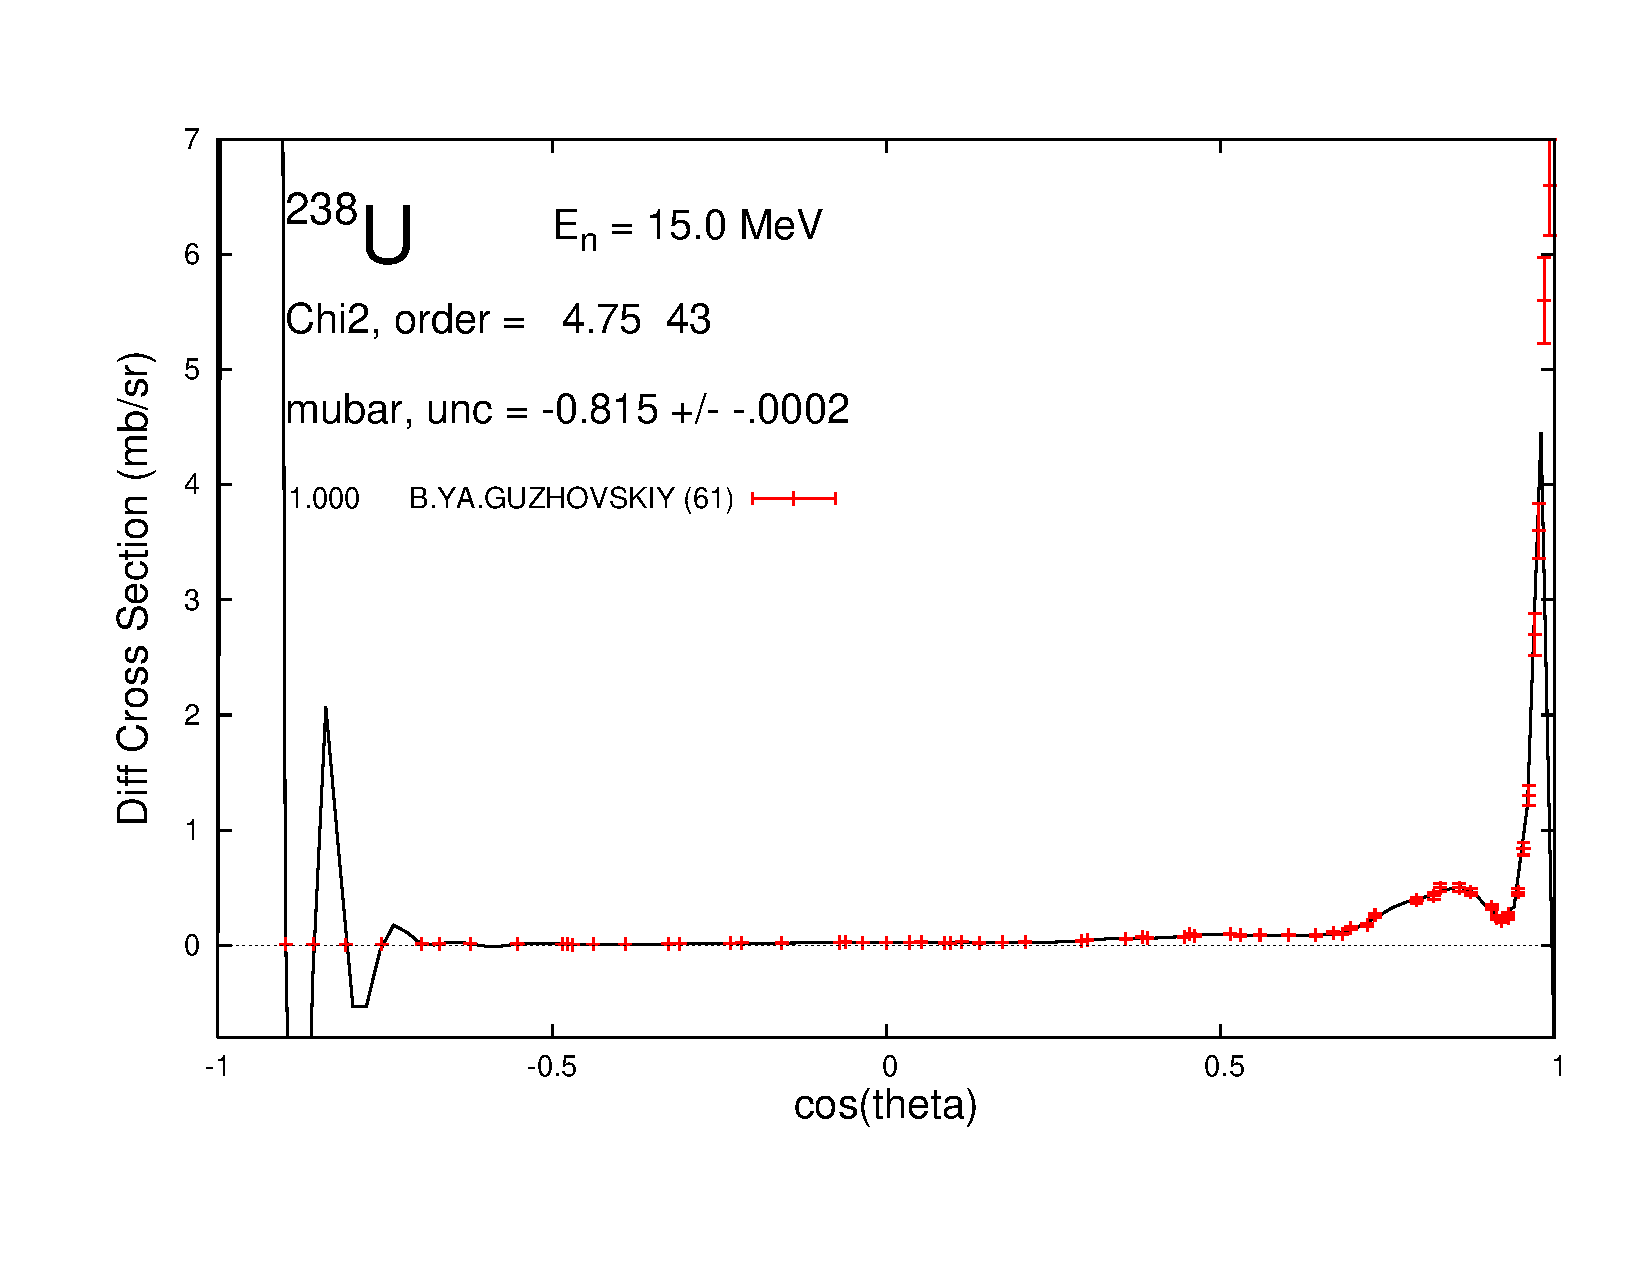
\includegraphics[trim = 15mm 15mm 0mm 0mm, clip,width=5.0in,angle=0.0]{figs/bad_mubar_high} \\
 \end{center}
 \vspace{-4mm}
 \caption{Legendre fit to differential cross section data at $E = 15$ MeV. Here the forward
 angle peak of the angular distribution requires a very high order Legendre polynomial for a
 good fit which results in a relatively good $\chi^{2}$ but the high oscillations at the
rather unconstrained backward angles result in a bad value for \mub\ of -0.815.}
 \label{Fig:bad_high}
\end{figure}
At high energy, it is often preferable to not fit the angular distribution but rather calculate
\mub\ directly, determining the the average cosine of the differential cross section as
\begin{equation}
\label{Eq:direct_mubar}
\bar{\mu} = \frac{\int_{-1}^{1} \frac{d\sigma(\theta)}{d\Omega} \cos\!\theta \, d\!\cos\!\theta}{\int_{-1}^{1} 
\frac{d\sigma(\theta)}{d\Omega} \, d\!\cos\!\theta}.
\end{equation}
For the distribution shown in Fig.~\ref{Fig:bad_high}, calculating \mub\ 
using Eq.~\ref{Eq:direct_mubar} results in a value of $0.82 \pm 0.03$, an acceptable
value, rather than the result from the high-order Legendre fit of $-0.815 \pm 0.0002$, which is clearly wrong.

Of course, to successfully use Eq.~\ref{Eq:direct_mubar} the angular coverage of the differential
cross section must be
sufficient to perform the integral. If this is not the case then
there is little choice but to use a Legendre fit. In any case, care must be always taken when
determining the value of \mub\ for a given elastic differential cross section. Each
fit must be visually inspected and only those that result in a good fit without problems (e.g.,
unconstrained or negative cross section, etc.) should be accepted for Kalman fitting. In the end, it
is up to the evaluator to decide which method provides the best value for \mub\ from a given
differential cross section. 
The accepted values with uncertainties are appended to the C4 file as MF154/MT2 data,
which are then paired with the EMPIRE cross predictions for \mub\ for fitting with Kalman. An
example of a set of \mub\ derived from $^{238}$U elastic differential cross sections,
with an EMPIRE calculation for \mub\ are shown in Fig.~\ref{Fig:empmu}.

\begin{figure}[htb]
 \begin{center}
  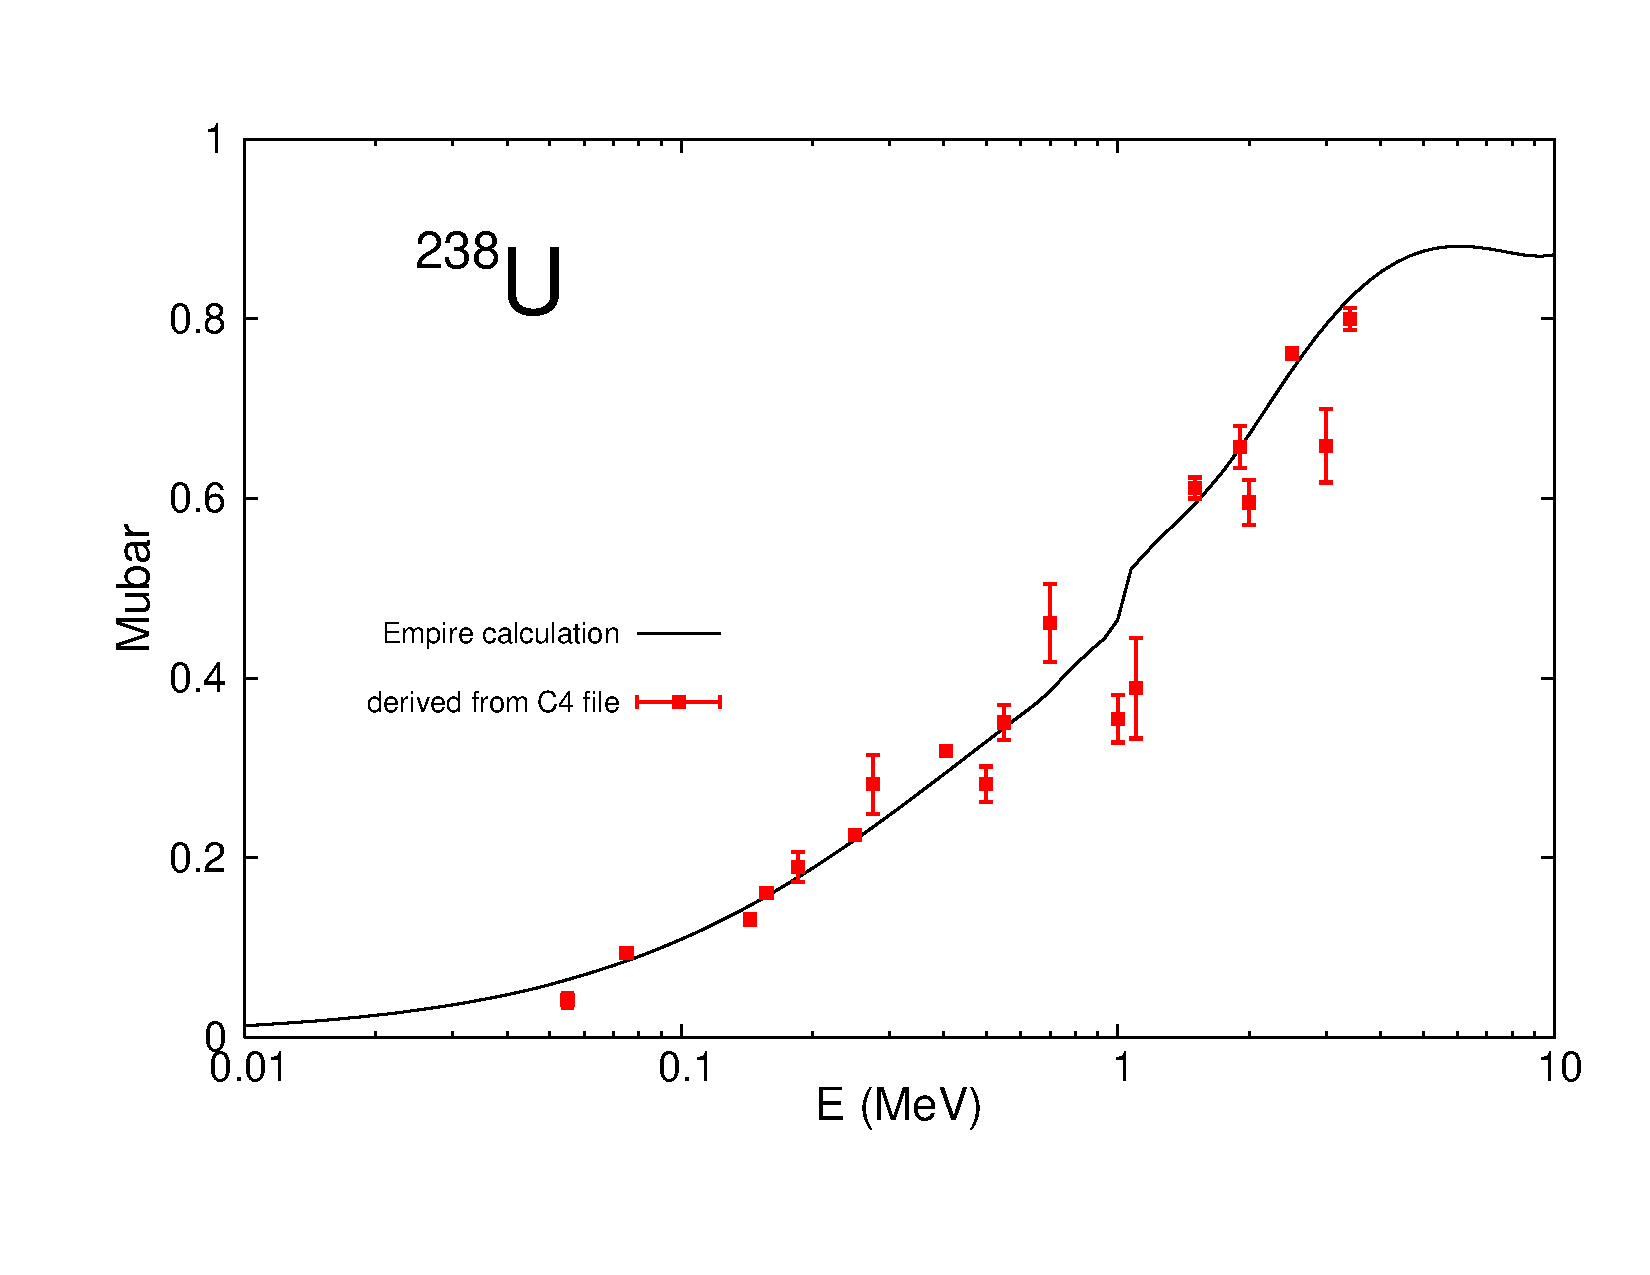
\includegraphics[trim = 15mm 15mm 0mm 0mm, clip,width=5.0in,angle=0.0]{figs/mubar_empire} \\
 \end{center}
 \vspace{-4mm}
 \caption{Values of \mub\ from fitted elastic differential cross sections for $^{238}$U shown
 in red with uncertainties from the fit. The black curve is an EMPIRE calculation for \mub.
 This curve is fit to the \mub\ data with the KALMAN code, which will adjust the EMPIRE 
 parameters based on their calculated sensitivities for \mub.}
 \label{Fig:empmu}
\end{figure}

The addition of calculated \mub\ to the list of cross sections output by EMPIRE required a minor
addition to the EMPIRE code. The differential cross sections are stored internal to EMPIRE
in the center-of-mass frame from $0^{\circ}$ to $180^{\circ}$, every $2^{\circ}$.
As \mub\ is defined as the average cosine of the elastic
scattered neutrons in the {\em Lab} frame, these differential cross sections are first boosted
to Lab and then the distribution is integrated using Eq.~\ref{Eq:direct_mubar} to
calculate \mub. This value is then written out to the *.xsc cross section file along with
the other cross sections used for fitting with KALMAN. It will later be mapped to MF3/MT251,
which is paired with \mub\ from the Legendre coefficients from fits to C4 data as MF154/MT2.

\subsection{\texorpdfstring{\nub}{Nubar} (Nubar)}

The number of neutrons produced per fission, \nub, can also be fit to data with the KALMAN
code. Here, the the values for \nub\ to be fit are directly available in the C4 data file
as MF1/MT452. These values need no further processing and are paired with the calculated
\nub\ from EMPIRE by the c4tokal.f90 routine. Care must be taken with fitting \nub\ as
EMPIRE does not calculate \nub\ but uses a distribution taken from an existing evaluated file, and scales it by
a single parameter. Therefore, fitting \nub should only be done when adjusting the scale
parameter in EMPIRE to fit new \nub\ data not being used by empire itself for \nub. In this
case, the KALMAN code can be used. The only parameter that will be adjusted is the \nub\
scaling parameter PFNNUI. This can be fit along with other cross section data or not. The
parameters for the cross sections do not affect \nub, so there will be no correlations
between the \nub\ scaling parameter PFNNUI and the other EMPIRE parameters. Of course, this
single scaling parameter can also be set by hand in this case, by taking the ratio of
the integral of the \nub\ spectrum used by EMPIRE to the integral of the \nub\ data being
fit.













\chapter{Evaluation procedure}





\chapter*{Acknowledgments}
\addcontentsline{toc}{chapter}{Acknowledgments}

EMPIRE is the result of an international cooperation towards open source
software, as so successfully promoted by the General Public License. A number
of authors contributed to the development of the code and it would be next
to impossible to list all names. We stress that the code described in this
paper would not have been possible without their valuable and voluntary
cooperation.


%Toshihiko, Raynal & inspirators
We are in debt to T. Kawano, who drew our attention to covariances and
who was actively involved in the implementation of his KALMAN code in EMPIRE. 
We owe very special thanks to J. Raynal who has been developing his ECIS
code since 1972~\cite{Raynal72} and is still actively maintaining and extending
it as evidenced by the recent release of the 2007 version. His code is the backbone of
EMPIRE, TALYS and McGNASH  for all optical model calculations,
playing a unique role in current nuclear data evaluation efforts. Another
special thanks go to the authors of GNASH (Mark Chadwick and Phil Young) as well
to the principal author of TALYS (Arjan Koning) for providing a never ending source
of inspiration to our continuous attempts to surpass performance and functionalities
of their codes.

%Said and Dave
We also highly appreciate S. Mughabghab's 
help in developing the resonance module linking his
Atlas of Neutron Resonances to
EMPIRE and D. Brown's  professional installation of  EMPIRE, which 
brings the code closer to the users.   

%main users 
First of all, we would like to acknowledge our colleagues whose work helped
to prepare this paper H. I. Kim, G. P. A. Nobre, A. Palumbo, and M. Pigni  deserve  
a special mention as the  major users of the code. Their 
comments were of great value and enabled us to trace coding errors, improve
stability and ease of use of the code. 

%IAEA
We feel particularly fortunate to be able to build on two solid
foundations - the comprehensive compilation of model parameters (RIPL) and
the extensive compilation of experimental results (CSISRS/EXFOR).
We are grateful to the recent heads of the IAEA Nuclear Data Section, Ch. Dunford, D.
Muir, A.L. Nichols and R. Forrest for their continued
support of the two projects. Naturally, our gratitude goes also to all
participants of the three phases of the RIPL project and to all EXFOR
compilers, in particular to V. McLane, S. Dunaeva and O. Schwerer, 
who dedicated their careers to EXFOR.
Three of us (M.H., R.C. and A.T.), who had  the privilege to
work under the leadership of A.L. Nichols, would like thank him for his
encouragement and support for the development of EMPIRE.

%contributors
We would like to thank A. Ventura who was involved in the early formulations
of the fission theory used in EMPIRE, E. B{\v e}t{\' a}k who developed exciton model
with angular momentum conservation used in earlier versions of EMPIRE, and to A.
Hoering who took part in the implementation of $\gamma $-emission within the 
Multi-Step Compound mechanism. 

We would like to thank A. Ignatyuk who has been a permanent source of
inspiration, constructive criticism and encouragement and lately has been
using EMPIRE in many different applications.

%'enlighteners'
Finally, there is a group of our colleagues to whom we owe particular
gratitude for their enlightenment and inspiration. It is a honour to
acknowledge H.A. Weidenm\"uller's guidance on multi-step compound theory and
the foundations of the statistical model, discussions with H. Lenske and H.
Wolter on the multi-step direct model and its implementation,
working with H. Hofmann on width-fluctuation corrections,
and with D. Smith on the exploration of the world of
covariances. EMPIRE would not have reached its current stage without
illuminating discussions on pre-equilibrium emission with M. Blann, P.E.
Hodgson, and E. Gadioli. We also benefited from the exchange of experience
with authors of other codes. We would like to express our appreciation to
S. Hilaire, P. Talou, and S. Goriely 
for inspiring discussions, indication of priorities, and technical
suggestions.

%nostalgy
One of us (M.H.) would like to thank A. Marcinkowski for motivating him to
write the EMPIRE-1 code. He is also grateful to G. Giardina and his
collaborators A. D'Arrigo, A. Lamberto, and A. Taccone who assisted the
EMPIRE-2 project from the very beginning and  tested  preliminary
versions of the code since 1993. Finally, we are indebted to R. Sturiale
for LINUX support at the early stages of the development of EMPIRE development. 
M.S. would like to express her gratitude to G. Vladuca for inspiring her interest in 
fission. 


%other code authors
Last but not least, we gratefully acknowledge the authors of the codes that are included in the
physics core of EMPIRE: 
M.B. Chadwick (DDHMS), 
H. Lenske and H. Wolter (ORION and TRISTAN), 
J. Raynal (ECIS), 
E. Soukhovitskii, S. Chiba, J.M. Quesada, O. Iwamoto, K. Shibata, T. Fukahori,
and G.B. Morogovskij  (OPTMAN), 
C.H. Dasso and S. Landowne (CCFUS), 
and A. Sierk (BARFIT and MOMFIT). 
Our gratitude goes also
to Ch. Dunford for his ENDF checking codes, D.E. Cullen whose suite of
preprocessing codes makes an essential part of the EMPIRE system and to R.
MacFarlane for his help in interfacing EMPIRE to his processing code NJOY.



%BNL
The work at BNL was sponsored by the Office of Nuclear Physics, Office of Science
of the U.S. Department of Energy under Contract No. DE-AC02-98CH10886 with
Brookhaven Science Associates, LLC. We are pleased to acknowledge strong support
by the International Atomic Energy Agency over last ten years.

\bibliographystyle{prsty}
\bibliography{scribus}



\appendix

\chapter{EMPIRE optional input keywords\label{InputList}}

The optional input allows modifications to the default model parameters. 
Optional input consists of an arbitrary number of records, entered in any order
and closed with the GO record, which indicates the end of the input. 
In the simplest case (all defaults), only the GO record must be entered. \\

Each optional record starts with an alphanumeric keyword {\bf NAME}. If the first 
character of the line (i.e. {\bf NAME(1:1)}) is {\bf *}, {\bf \#} or {\bf !}, then this
line contains comments and is ignored by the code. There might be an arbitrary number of
comments line in the optional input. If the first character of the line {\bf NAME(1:1)} 
is {\bf @}, then this line contains a title, which will be printed in EMPIRE outputs; 
obviously the title is not used in any calculations. Multiple titles are allowed. 
Users are strongly encouraged to use titles and comments in EMPIRE inputs; that will be a 
significant step toward a better documentation of our theoretical calculations 
and evaluations.\\

The optional-input keyword {\bf NAME} is followed by the value VAL and four positional
parameters I1, I2, I3, I4. The keyword indicates a physical quantity, such as the
binding energy or level density parameter or scaling parameter. 
VAL takes the numerical value  of the given quantity or scaling parameter.  \\
The  positional parameters are typically  used to  specify to which nucleus the quantity 
should be applied (generally  if these are omitted  the value is applied to all
nuclei in the given calculation). Positional parameters may be also used to 
indicate the estimated uncertainty of the quantity defined by the input keyword 
(except optical model parameters for which the uncertainty is defined by VAL). 
Each record must be in the FORTRAN format:\\
\begin{quote}
FORMAT (A6,G10.5,4I5) {\bf NAME},VAL,I1,I2,I3,I4
\end{quote}
%\\
Fixed format allows to avoid typing zeros if no input is needed for some 
positional parameters.

The GO record indicates end of the optional input and starts calculations. 
It may be followed by an unlimited list of incident energies (and titles or comments)
(one per record) terminated with a record containing a negative value.
Anything below this line will be ignored by the code. 

\section*{Calculation control}

\begin{description}[style=multiline,leftmargin=3cm]
\item [{NEX}] Maximum number of energy steps in the integration set to
VAL (default: min(50, NDEX)). NDEX parameter is defined in the \emph{dimension.h} file.
\item [{ENDF}] Controls output for ENDF formatting and exclusive/inclusive emission

= 0 no  ENDF formatting (default).
  
    
$>0$ output for the full ENDF formatting will be created (including double differential MF=6) as shown in the two examples below

                ~~~~= 2 means all reactions emitting 2 or less particles are exclusive
                
                   ~~~~~~~~~the rest are inclusive (lumped into MT=5)
                     
                ~~~~= 3 means all reactions emitting 3 or less particles are exclusive
                
                     ~~~~~~~~~the rest are inclusive (lumped into MT=5)
                     
\item [{RECOIL}] Controls calculation of recoils,

= 0 recoils are not calculated (default if ENDF = 0, no ENDF formatting)

= 1 recoils are calculated     (default if ENDF $>0$, ENDF formatting)

If keyword ENDF=0 is given in the input, then recoils are not calculated
independently of the keyword RECOIL.

\item [{PRGAMM}] Controls calculation of primary gammas

= 0 Primary gammas are not printed (default)

$>1$ Primary gammas are  printed

If keyword ENDF=0 is given in the input, then primary gammas are not
printed independently of the keyword PRGAMM.

\item [{GAMPRN}] Controls printing of gamma production cross sections (n,xng)

= 0 Gamma production cross sections are not printed (default)

$>0$ Gamma production cross sections files and plots are produced.

\item [{HRTW}] Controls HRTW calculations (width fluctuation correction)

= 0 no HRTW 

$>0$ HRTW width fluctuation correction up to the energy set by VAL. 

\item [{FISSPE}] Controls calculation of prompt fission neutron spectra (PFNS).

= 0 PFNS are not calculated (default)

= 1 PFNS are calculated using Los Alamos model \cite{Madland:82}

= 2 PFNS are calculated using Kornilov parameterization \cite{Kornilov:99}

\item [{CNANGD}] Controls calculation of CN angular distribution.

= 0 Compound nucleus (CN) angular distribution assumed isotropic (default)

> 0 Compound nucleus (CN) angular distribution assumed anisotropic;
    collective levels must be present and DIRECT>0.

\item [{INTERF}] Controls calculation of interference effects between direct 
    and compound decay.

= 0 Compound nucleus (CN) and direct cross section are added incoherently (default)

= 1 Compound nucleus (CN) and direct interference considered by Engelbrecht-
      Weidenmuller transformation (see Phys.Rev. C8(1973)859-862). Collective
	  levels must be present and DIRECT>0.

\item [{FISSPE}] Controls calculation of prompt fission neutron spectra (PFNS).

= 0 PFNS are not calculated (default)

= 1 PFNS are calculated using Los Alamos model \cite{Madland:82}

= 2 PFNS are calculated using Kornilov parameterization \cite{Kornilov:99}



\item [{BENCHM}] Controls if benchmark calculation is requested. 

= 0 no benchmark calculation (default),

$>0$ benchmark calculation requested. Energies do not need to be in increasing order.

\item [{KALMAN}] Controls calculation of a sensitivity matrix,

= 0 no sensitivity matrix  calculations (default),

= 1 sensitivity matrix is calculated.

\item [{RANDOM}] Controls randomization of input parameters that were input with uncertainty
\begin{description}

\item[= 0] no random sampling is allowed (default) 

\item[$>0$] random sampling based on normal (Gaussian) distribution with the given 1-sigma parameter uncertainty 

\item[$<0$] random sampling based on uniform distribution with the given 1-sigma parameter uncertainty 
\end{description}

\item [{ISOMER}] The minimum isomer half life (in seconds) set to VAL

This keyword defines minimum half-life of the state to be considered an isomer (default 1. = 1 second)

\end{description}

\section*{Output control}

\begin{description}[style=multiline,leftmargin=3cm]
\item [{IOUT}] Main output control set to VAL 
\begin{description}[style=multiline,leftmargin=1cm]
\item[= 1] input data and essential results (all cross sections) (default),
\item[= 2] as IOUT=1 plus fusion spin distribution, yrast state population,
$\gamma$-transition parameters, fusion barrier, inclusive spectra,
\item[= 3] as IOUT=2 + $\gamma$ and particle spectra + discrete levels'
decay + double differential cross sections (if MSD\index{MSD}$>$0),
\item[= 4] as IOUT=2 + ORION\index{ORION} output + residual nuclei continuum
population (up to spin 12), 
\item[= 5] as IOUT=2 + ORION output + transmission coefficients (up to l=12),
\item[= 6] as IOUT=2 + ORION output + level densities\index{level densities}
(up to spin 12). Should be used to get ZVV level density plots.
\end{description}

\item [{NOUT}] MSC\index{MSC} calculation output control set to VAL (default:
0).
\end{description}

\subsubsection*{Optical Model Potential }

\begin{description}[style=multiline,leftmargin=3cm]

\item [{OMPOT}] Selects optical model parameters for outgoing particle 

        The value of I1 selects the outgoing particle as follows: 
        
        =1 neutrons, 
        
        =2 protons, 
        
        =3 alphas, 
        
        =4 deuterons, 
        
        =5 tritons, 
        
        =6 He-3; 
        
        VAL must be set to a RIPL catalog number (e.g. 2408 for Capote et al OMP)
        of the potential as it appears in the empire/RIPL/optical/om-data/om-index.txt
        file or in Help $=>$ 'RIPL omp' when using GUI. For backward compatibility this
        number can be entered with a negative sign.

\item [{DIRPOT}] Optical model parameters to be used in DWBA or coupled-channels calculations by ECIS/OPTMAN codes. Parameters are the same as above, except that I1 need not be specified (always refers to the incident channel).
        
\item [{RELKIN}] Override the RIPL defined kinematics used in a given optical model potential,

       = 0 classical (default),
       
       = 1 relativistic.

\item [{TRGLEV}] Excited level of the target is set to VAL  (e.g., VAL=3 for the 2$^{nd}$ excited state; default: 1 (ground state)).

\item [{UOMPab}] 
 Uncertainty of the parameters defining the potential strength 
of the optical model potential. The letter a can be V (real potential strength) or W 
(imaginary potential strength). The letter b can be V (volume) or S(surface).
Thus the combinations VV (real volume), WV (imaginary volume), and WS (imaginary surface) 
specify 3 different terms in the RIPL optical potential described in Refs.~\cite{RIPL2,RIPL3}. 
The combination VS is not allowed, as parameters of the real surface potential (VS) are usually
not used in deriving phenomenological potentials. The exception is for dispersive potentials, but
in this case the VS uncertainty is fully determined by the uncertainty of the imaginary surface
potential (WS). The uncertainty of the spin-orbit potential is also not considered as its influence on calculated
cross sections is small.\\
The relative uncertainty in \% of the corresponding parameter (defined by letters \emph{a} and \emph{b}) is given by VAL, 
 target's  Z and  A numbers are defined by I1 and I2, respectively. 
I3 defines the outgoing particle, i.e., the incident particle for the inverse reaction (I3=1 for 
neutron, I3=2 for protons, etc). \\
Some examples of potential strength uncertainties are given below.
\begin{verbatim}
* The three lines below define 1.5% uncertainty of the real 
* volume potential strength and 10% uncertainty of the real 
* and imaginary surface potential strength for neutron and 
* proton emission channels from the 56-Mn compound nucleus
UOMPVV   1.50000  25    55   1  
UOMPWV  10.0000   25    55   1   
UOMPWS  10.0000   25    55   1 
* The same for the proton emission channel
UOMPVV   1.50000  24    55   2    
UOMPWV   2.5000   24    55   2    
UOMPWS  10.0000   24    55   2    
\end{verbatim}


\item [{UOMPcd}] Defines the uncertainty of the geometry component of the optical model
potential. The letter c can be R (radius) or A (diffuseness). The letter d can be V (real volume),
W (imaginary volume) or S (imaginary surface). Thus the following six combinations are possible:
RV and AV (real volume radius and diffuseness), RW and AW (imaginary volume radius and diffuseness),
and RS and AS (surface radius and diffuseness). \\
The relative uncertainty of the corresponding parameter (defined by letters c and d) is given by VAL 
(in percent),  target's  Z and  A are defined by I1 and I2, respectively. 
I3 defines the outgoing particle, i.e. the incident particle for the inverse reaction (I3=1 for 
neutron, I3=2 for protons, etc). \\
It is recommended to avoid variations of potential strength (e.g. VV,WV) and corresponding potential 
radius (e.g. RV, RW) in the same run, as those parameters are strongly correlated within the optical
model.\\
Some examples of geometry uncertainties of the optical model parameters are given below.\\
\begin{verbatim}
* The two lines below define 1.5% uncertainty of the   
* imaginary volume radius, and 2.5% uncertainty of the  
* imaginary volume diffuseness for a neutrons incident 
* on 55Mn nucleus
UOMPRW   1.50000  25    55   1    
UOMPAW   2.5000   25    55   1    
* The same for the proton emission channel  
* corresponding to the surface potential.
UOMPRS   1.50000  24    55   2    
UOMPAS   2.5000   24    55   2  
\end{verbatim}
  

\end{description}

\section*{Scattering on collective levels}
EMPIRE includes two coupled-channels codes: ECIS\index{ECIS} and
OPTMAN\cite{OPTMAN1,OPTMAN2,OPTMAN3}. ECIS is the default optical model solver,
but OPTMAN should be used for selected potentials, when soft-rotor 
couplings are desired, as well as for actinide potentials that couple levels
beyond the ground state rotational band.

\begin{description}[style=multiline,leftmargin=3cm]
\item [{DIRECT}] Controls use of coupled-channel calculations (ECIS and OPTMAN) 

\begin{description}[style=multiline,leftmargin=1cm]

\item[=0] spherical OM used (default) 

\item[=1] Coupled Channel (CC) method used for calculation of inelastic scattering
to collective levels in the incident channel. 
If a selected OM potential is of CC type, the elastic and reaction cross 
sections are also taken from ECIS/OPTMAN calculations. 
Otherwise, spherical OM results are used. Transmission coefficients
for all outgoing channels are calculated with spherical OM. 

\item[=2] as above but transmission coefficients for the inelastic outgoing
channels are calculated within Coupled Channel approach (longer calculation time). 

\item[=3] as DIRECT=1 but DWBA\index{DWBA} is used instead of CC for calculation of 
inelastic scattering to collective levels in the incident channel. 
All transmission coefficients calculated with spherical OM. 
\end{description}

NOTE: OM potential to be used by ECIS/OPTMAN might be different from the
one used in the rest of the calculations and can be specified with
the DIRPOT option.

\item [{CALCTL}] Controls use of calculated transmission coefficients for both 
projectile and ejectiles.\\

\begin{description}[style=multiline,leftmargin=1cm]

\item[= 0] Transmission coefficients calculated during the first run are stored, and reused
    in subsequent EMPIRE runs (default),
       
\item[$>0$] Transmission coefficients are calculated for each run even if they were calculated before and respective files  exist. This option is useful to calculate some quantities that are only used if TL are not already present (e.g. Bass fusion barrier in HI induced reactions).

    NOTE: this option slows down the execution of the code in subsequent runs by
    up to a factor of 10  (additional time is needed to calculate TLs again; reading
    them is much faster).
\end{description}

\item [{EcDWBA}] Automatically selects all discrete levels to be used in DWBA
calculations for uncoupled collective levels. \\
The default cut-off energy is $3*30/A^{2/3}$, and the default maximum spin 4. 
With these defaults all levels ($J<5$) with excitation energy less than 
2.4 MeV for $^{238}U$), and  less than 6.2 MeV for $^{56}Fe$ are considered.\\
The default selection rules could be modified by the VAL parameter that redefines
the cut-off energy, and the parameter I1 that sets the maximum spin. 

\item [{RESOLF}] Energy resolution in MeV used to spread calculated collective 
cross sections in the continuum set to VAL.\\
This parameter is used if there are collective levels (in the {*}-lev.col file)
that are located in the continuum (see the \emph{cont} flag). The scattering
cross sections on these levels will be calculated by DWBA (if keyword DIRECT $>0$).

\item [{DEFNUC}] Deformation of the target nucleus set to VAL.\\
The threshold value to assume that the nucleus is deformed is 0.1
If you want to force the assumption of sphericity for a given nucleus
you can use this parameter with a value less than 0.1
this parameter also affects the deformation used in MSD calculations.        

\item [{ECONT}] The energy continuum for the nucleus with Z=I1 and A=I2
starts at energy given by VAL in MeV.\\
This parameter overwrites the continuum cut-off energy defined in the 
default RIPL levels for a given nucleus (or even the value given in the
local LEVELS file). If not nucleus is given, then the value is ignored. 

\end{description}

\section*{Scaling parameters correcting for model deficiencies}
These parameters are non-physical parameters designed to be used in nuclear data evaluation to correct for reaction model deficiencies, and to define model parameters' uncertainties.
They are also used for covariance calculations by providing a straightforward way to calculate sensitivities (required as input for KALMAN), and to allow for random sampling of model parameters within defined uncertainties (required for Monte Carlo generation of theoretical model covariances). 


\begin{description}[style=multiline,leftmargin=3cm]
\item [{TUNE}] The equilibrium decay width $\Gamma^{EQ}_i$ of the ejectile $i$ given by I3,
for the nucleus with Z=I1 and A=I2 will be multiplied by VAL.\\
Estimated relative uncertainty in \% of this parameter can be given by I4.

\item [{TUNEFI}] The fission decay width $\Gamma_F$ will be multiplied by VAL for the nucleus with Z=I1 and A=I2.\\ 
Estimated uncertainty of this parameter can be given by I3.

\item [{TUNEPE}] The preequilibrium decay width $\Gamma_i$ of the ejectile $i$ 
given by I1 will be multiplied by VAL. It applies only to the PE decay from the
compound nucleus calculated by PCROSS (exciton model), input keyword PCROSS $>0$. \\
Estimated relative uncertainty in \% of this parameter can be given by I2.

\item [{PFNNIU}] Used in prompt fission neutron (PFN) calculations.
                 The evaluated total prompt neutron multiplicity $\widetilde{\nu}$
                 (read from NUBAR-EVAL.ENDF) will be multiplied by VAL (default: 1.).
                 The relative uncertainty of the scaling factor in \% could be given by I1.\\
 
\item [{PFNTKE}] Used in prompt fission neutron (PFN) calculations.
                 The total kinetic energy (TKE) of the fission fragments
                 will be multiplied by VAL (default: 1.).
                 The TKE enters the energy balance equation defining the total excitation
                 energy of the fissioning system $U_{exc} = E_{rel} - TKE + E_{incid} + B_n$.
                 This parameter could be interpreted as the uncertainty of the measured
                 fission kinetic energy.\\
                 The relative uncertainty of the scaling factor in \% could be given by I1.
                
\item [{PFNALP}] Used in prompt fission neutron (PFN) calculations.
                 The default parameter $\alpha$ ($\alpha_0=1$ for Madland-Nix (LA) model~\cite{Madland:82} and
                 $\alpha_0~0.9$ for Kornilov parameterization~\cite{Kornilov:99}) will be multiplied by VAL (default: 1.).
                 The values $E_f^L$ and $E_f^H$ of the average kinetic energy per nucleon
                 of the average light fragment AL and average heavy fragment AH are scaled
                 by $\alpha$. The effect of this parameter on PFNS calculations is strongly correlated
                 with TKE (see keyword PFNTKE above). //
                 Physically, this parameter allows for a reduction of the kinetic energy of the
                 fragment due to neutron emission during Coulomb acceleration.\\
                 The relative uncertainty of the scaling factor in \% could be given by I1.\\
 
\item [{PFNRAT}] Used in prompt fission neutron (PFN) calculations.
                 The default parameter $r=T_f^L/T_f^H$ ($r_0=1$ for Madland-Nix (LA) model~\cite{Madland:82} and
                 $r_0=1.248$ for Kornilov parameterization~\cite{Kornilov:99}) will be multiplied by VAL (default: 1.).
                 This parameter defines the ratio of temperatures of the light to heavy fragment.
                 Experimental evidence strongly supports ~20\% higher temperature of the light fragment.\\
                 The relative uncertainty of the scaling factor in \% could be given by I1.\\
                
\item [{PFNERE}] Used in prompt fission neutron (PFN) calculations.
                 The total fission energy release ($E_{rel}$) will be multiplied by VAL (default: 1.).
                 The $E_{rel}$ enters the energy balance equation defining the total excitation
                 energy of the fissioning system $U_{exc} = E_{rel} - TKE + E_{incid} + B_n$.
                 The relative uncertainty of the scaling factor in \% could be given by I1.

\item [{TMAXW}]  Used in prompt fission neutron (PFN) calculations.
                 PFNS plots are scaled by a Maxwellian function with T = VAL (default: 1.32) MeV.

\item [{DEFSTA}] The static deformation needed in rigid-rotor CC calculations
                 will be multiplied by VAL (default: 1.).\\
                 The relative uncertainty of the scaling factor in \% could be given by I1.\\
                 It is recommended not to vary dynamical deformation above 10 MeV 
				 (i.e. set its uncertainty to zero) to avoid numerical instabilities.

\item [{DEFDYN}] Dynamical deformations of uncoupled levels for DWBA calculations will be 
                 multiplied by VAL (default: 1.).\\
                 Dynamical deformations are listed for all collective levels in the collective 
                 file ({*}-col.lev).\\ 
                 The relative uncertainty of the scaling factor in \% could be given by I1.\\
                 It is recommended not to vary dynamical deformation above 10 MeV 
				 (i.e. set its uncertainty to zero) to avoid numerical instabilities.

\item [{ELARED}] The shape elastic cross section will be multiplied by VAL (default: 1.).
                 The change is also reflected in the total cross section. \\
                 The relative uncertainty of the scaling factor in \% could be given by I1.

\item [{FUSRED}] The fusion (reaction) cross section will be multiplied by VAL (default: 1.).
                 The change is also reflected in the total cross section. \\
                 The relative uncertainty of the scaling factor in \% could be given by I1.

\item [{FCCRED}] The calculated direct cross section for discrete collective levels will be multiplied
                 by VAL (default: 1.). Cross sections of both coupled and uncoupled discrete levels are 
				 scaled. \\
                 The uncertainty of the scaling factor in \% could be given by I1.\\
                 It has no effect if DIRECT keyword is set to zero in the input (default).

\item [{FCORED}] The DWBA calculated direct cross section for collective levels in the continuum will
                 be multiplied by VAL (default: 1.). Giant multipole resonances are also scaled
				 if specified in the collective level file (flagged with negative deformation). \\
                 The uncertainty of the scaling factor in \% could be given by I1.\\
                 It has no effect if DIRECT keyword is set to zero in the input (default).\\
				 A value of zero could be used to supress DWBA collective levels in the continuum,
				 without recalculating the transmission coefficients (TLs).

\item [{TOTRED}] The total cross section will be multiplied by VAL (default: 1.). \\
                 The relative uncertainty of the scaling factor in \% can be given by I1.\\
				 TOTRED is applied through other scaling factors, namely ELARED,FUSRED,FCCRED and FCORED.\\
				 If those factors are present, then the final scaling will be a product of them 
				 (e.g., if both TOTRED and FUSRED are specified, then the fusion (reaction) cross section
				 will be multiplied by FUSRED*TOTRED.\\
This parameter is recommended to be used to correct small deficiencies (~3\%) of your optical model 
calculated total cross sections. It is not recommended to be used for simulation of the experimental fluctuations
of total cross section.

\item [{CELRED}] The compound elastic cross section will be multiplied by VAL (default: 1.). \\
                 The relative uncertainty of the scaling factor in \% can be given by I1.\\
This parameter may be used to simulate the CN resonances (obviously not included in the optical model), or  
to simulate physical effects arising from the compound-direct processes interference
(Engelbrecht-Weidenmuller transformation). The interference increases the compound inelastic cross sections,
reducing others compound channels (incl. the compound elastic). It is recommended to avoid using CELRED and CINRED
at the same energy as they affect the same quantities.

\item [{CELCOR}] The compound elastic cross section will be multiplied by VAL (default: 1.). \\
                 The relative uncertainty of the scaling factor in \% can be given by I1.\\
This parameter may be used for a simple scaling of the CE cross section, without affecting compound
inelastic cross sections.

\item [{CINRED}] The compound inelastic cross section to discrete levels will be multiplied by VAL (default: 1.). \\
                 The discrete level number can be given by I1.\\
                 The relative uncertainty of the scaling factor in \% can be given by I2.\\
This parameter may be used to simulate physical effects arising from the compound-direct processes interference
(Engelbrecht-Weidenmuller transformation). The interference increases the compound inelastic cross sections,
reducing others compound channels (incl. the compound elastic). 

\item [{DXSRED}] The calculated deuteron pick-up/stripping cross section for incident deuteron on the target
                 nucleus will be multiplied by VAL). 
                 It has no effect on other incident particles. 
                  
              \begin{description}[style=multiline,leftmargin=1cm]
               \item[$>0$] deuteron pick-up/stripping parameterization of Kalbach used for incident deuterons (default: 1.),
               \item[$=0$] deuteron pick-up/stripping suppressed.  
              \end{description}

\end{description}

\section*{Optical model fitting}

\begin{description}[style=multiline,leftmargin=3cm]
\item [{FITOMP}] Controls fitting of optical model potential in the incident channel, 

        \begin{description}
        \item [=0] No fit (default)
        
        \item [=1] GUI assisted manual fitting; independently of what is specified in the input only total, elastic, capture and inelastic scattering are calculated.  If plots with 'List names' ompR1 and eventually ompR2 are set they will be updated and reproduced after each run.
        
        \item [=2] Automatic fit. See default EMPIRE input (../scripts/skel.inp) or the description 
           of the parameter FITabc below for keywords to be placed in the input. 
       \end{description}
        
\item [{FITabc}] Selects an optical model parameter for adjustment. The
letter a can be R (real) or I (imaginary) and the letter b can be
V (volume), S (surface) or O (spin-orbit). Thus the combinations RV,
IV, RS, IS, RO and IO specify the 6 different terms in the RIPL
optical potential described in Refs.~\cite{RIPL2,RIPL3}. The letter
c can be V (potential strength), R (radius) or D (diffuseness). The
initial shift in the parameter is given by VAL and the maximum allowed
variation is given by 0.01{*}I1. I2 specifies which of the parameters
in the potential strength, radius or diffuseness is to be adjusted.\\
           Some examples are given below.\\
   \begin{verbatim}
FITRVV     0.     500    1    !fit real volume depth (+- 5 MeV)
FITIVV     0.     100    1    !fit imag. volume depth (+- 1 MeV)
FITISV     0.     100    1    !fit imag. surface depth (+- 1 MeV)
FITRVR     0.      10    1    !fit real volume radius (+- 0.1 fm)
FITIVR     0.      10    1    !fit imag. volume radius (+- 0.1 fm)
FITRVD     0.      10    1    !fit real volume diffus. (+- 0.1 fm)
FITISD     0.       5    1    !fit imag. surf. diffus. (+- 0.05 fm)
\end{verbatim}

\item [{FITDEF}] Selects the deformation parameter of multipole I2 for
adjustment. The initial shift in the parameter is given by VAL and
the maximum allowed variation is given by 0.01{*}I1. The value of
I2 can be 2 or 4 for rotational nuclei and 2 or 3 for vibrational
nuclei, e.g.,
\begin{verbatim}
FITDEF     0.      10    2    !fit l=2 (quadrupol) defor. (+- 0.1)
\end{verbatim}

\item [{FITWT}] Multiplies weights of experimental data of type MF=I1 and
MT=I2 in $\chi^{2}$ by VAL.

\item [{FITWT0}] Multiplies weights of natural element experimental data
in $\chi^{2}$ by VAL.

\item [{FITITR}] Sets the number of iterations in the gradient $\chi^{2}$
minimization to\\ VAL=maxitr+0.01{*}itmax, \\where maxitr is the number
of times the gradient is calculated and itmax is the number of iterations
along each gradient (default is 3.05).

\item [{FITEMX}] Maximum incident energy of experimental data used in fitting
set to VAL (default is 30 MeV).

\item [{FITGRD}] Defines the initial grid of incident energies of nuclear
model calculations used to obtain $\chi^{2}$. When set, the first
interval is VAL, the second VAL +0.001{*}I1, the third VAL+0.002{*}I1,
etc. (The default incident energy grid is the one given in the input
file.) 
\end{description}

\section*{Fusion\label{sec: InpFus}}
These input parameters are typically used for heavy ion induced reactions.\\
\begin{description}[style=multiline,leftmargin=3cm]
\item [{CSREAD}] Controls HI fusion cross section determination,

$>0$ HI fusion cross section is set to VAL {[}in mb], 

= -1 distributed barrier model used ,

= -2 simplified coupled-channel treatment  CCFUS-code (default for HI).
 
 Note: CSREAD has no effect if .\emph{fus} file (\emph{FUSION} in
manual mode) exists.
\item [{BFUS}] Fusion barrier height in the distributed barrier model (Eq.~\ref{distbarr}) set to VAL (default: $B_{fus}$ calculated by CCFUS\index{CCFUS}).
\item [{SIG}] SIGMA in the distributed barrier model (Eq.~\ref{distbarr})
set to VAL (default: $0.05B_{fus}$).
\item [{TRUNC}] Truncation in the distributed barrier model (Eq. \ref{distbarr})
set to VAL (default: 2.).
\item [{EXPUSH}] Extra-push energy set to VAL (default: 0.).
\item [{CRL}] Critical \emph{l}-value for HI fusion (Eq. \ref{Tlfus})
set to VAL (default: 0).
\item [{DFUS}] Diffuseness in the transmission coefficients for HI fusion
(Eq. \ref{Tlfus}) set to VAL (default: 1.).
\end{description}

\section*{Photo-absorption}

\begin{description}[style=multiline,leftmargin=3cm]
\item [{E1}] = 0 E1 photo-absorption blocked

= 1 E1 photo-absorption selected
\item [{M1}] = 0 M1 photo-absorption blocked 

= 1 M1 photo-absorption selected
\item [{E2}] = 0 E2 photo-absorption blocked 

= 1 E2 photo-absorption selected
\item [{QD}] Quasideuteron photo-absorption cross section normalized by
a factor VAL 
\end{description}

\section*{CCFUS\index{CCFUS} input}

CCFUS code provides a simplified coupled-channel treatment to obtain 
the reaction cross section in near-barrier heavy ion reactions. 
It is not recommended for reactions with light incident particles ($A<5$).\

\begin{description}[style=multiline,leftmargin=3cm]
\item [{DV}] DV barrier parameter in CCFUS set to VAL. This parameter can
be used to adjust the fusion barrier. Typical range for changes $-10<DV<10$.
(default: 10).
\item [{FCC}] FCC parameter in CCFUS\index{CCFUS} set to VAL
\begin{description}[style=multiline,leftmargin=1cm]
\item[=0] diagonalization of the coupling is performed at the barrier position
$r_{b}$,
\item[=1] exponential character of the form factor is taken into account.
A second order estimation of the position and height of the effective
barriers is carried out within a one-Fermi distance from $r_{b}$.
This option is recommended for strong coupling (default). 
\end{description}

\item [{NSCC}] Number of inelastic surface channels in CCFUS\index{CCFUS}
set to VAL (default: 4).
\item [{NACC}] Number of additional channels set to VAL (default: 0).
\item [{BETCC}] Deformation of the I2$^{th}$ collective mode set to VAL.
\item [{FLAM}] Multi-polarity of the I2-th collective mode set to VAL (entered
with positive sign for target modes and negative sign for projectile
modes) (default:~ 2, 3, -2, -3, needs NSCC numbers).
\item [{QCC}] Q-value of the I2$^{th}$ collective channel set to VAL -
excitation energy of the collective level adopted with a negative
sign (default: - energies of the first 2+ and 3- levels in the target
and the projectile). 
\item [{FCD}] Strength of the coupling at the barrier for I2$^{th}$ collective
mode set to VAL. For FCC=1 the characteristic radial dependence of
the one-particle transfer form factor is assumed. Used only if NACC$>0$
(no default).
\end{description}


\section*{Multi-step Direct}

\begin{description}[style=multiline,leftmargin=3cm]

\item [{MSD\index{MSD}}] Controls Multi-step Direct\index{MSD} calculations,
\begin{description}
\item[= 0] no MSD calculations (default),
\item[= 1] MSD calculations selected - ORION\index{ORION} + TRISTAN\index{TRISTAN} will be executed,
\item[= 2] MSD calculations selected including the MSD contribution to discrete levels. 
This option should be used with care if coupled channel optical model potentials
are employed. Since MSD gives the vibration component of the direct cross section it sometimes it might be summed with the rotational CC contribution but summing it with the vibrational CC one would be an obvious double-counting.
\end{description}

\item [{MSDMIN}] The minimum energy to start MSD calculations set to VAL (default: 5.).\\

\item [{DEFMSD}] Deformation $\beta_2$ of the Nilsson Hamiltonian set to VAL (default: 0.).\\
  The Nilsson hamiltonian is used to obtain single-particle levels employed in MSD calculations.  

\item [{WIDEX}] Experimental energy resolution set to VAL (default: 0.2).
\item [{GAPP}] Proton pairing gap for target set to VAL (default: $12/\sqrt{A}$).
\item [{GRANGP}] Energy window around the $E^p_F$ for proton pairing calculations 
      for target set to VAL (default: 5.).
\item [{GAPN}] Neutron pairing gap for target set to VAL (default: $12/\sqrt{A}$).
\item [{GRANGN}] Energy window around the $E^n_F$ for neutron pairing calculations 
      for target set to VAL (default: 5.).
\item [{HOMEGA}] $\hbar\omega$ oscillator energy (default: 41.47/A$^{1/3}$
MeV ).
\item [{EFIT}] Coupling constants of multi-polarity I1 fitted to the level
at energy VAL (defaults: -1 for $\lambda=0$, $E_{GDR}$ for $\lambda=1$,
energies of the first low-lying 2+, 3-, and 4+ levels for $\lambda=2,\,3,\,4$,
respectively).
\item [{RESNOR}] Response function for multi-polarity I1 will be normalized
by factor VAL (default: 1).
\item [{ALS}] spin-orbit coupling strength in the harmonic oscillator (default: 1.5).

\end{description}

\section*{Multi-step Compound }

\begin{description}[style=multiline,leftmargin=3cm]

\item [{MSC\index{MSC}}] Controls Multi-step Compound\index{MSC} calculations,

= 0 no MSC calculations (default),

= 1 MSC calculations selected.

\item [{XNI}] Initial exciton number set to VAL (default set internally
depending on the case, 3 for nucleon induced reactions).

\item [{GDIV}] Single particle level densities in preequilibrium models
(MSC, DTRANS, PCROSS) set to A/VAL (default: 13.0).

\item [{TORY}] Ratio of unlike to like nucleon-nucleon interaction cross
section set to VAL. Used for the determination of the relative share
between neutron and protons in the exciton configurations (default:
4.).

\item [{EX1}] Initial number of excitons that are neutrons set to VAL (default
set internally depending on the case and on TORY).

\item [{EX2}] Initial number of excitons that are protons set to VAL (default
set internally depending on the case and on TORY).

\item [{D1FRA}] Ratio of the spreading GDR width to the total GDR width
set to VAL (default: 0.8).

\item [{GST}] Controls $\gamma$-emission in MSC\index{MSC},

= 0 no $\gamma$-emission in MSC (default),

= 1 $\gamma$-emission in MSC selected.

\item [{STMRO}] =0 closed form \emph{p-h} state densities selected (default)\\
\end{description}

\section*{Monte Carlo pre-equilibrium model (HMS\index{HMS}) }

\begin{description}[style=multiline,leftmargin=3cm]
\item [{HMS}] Controls Monte Carlo pre-equilibrium calculations,

= 0 HMS disabled (default),

= 1 HMS enabled.
\item [{NHMS}] Number of events in HMS set to VAL
\item [{CHMS}] Default damp rate in HMS multiplied by VAL
\item [{FHMS}] Transition densities used in HMS set by VAL

= 0 Exciton densities are used,

= 1 Fermi gas densities are used,

= 2 Exact NR Fermi gas densities are used,

= 3 Exact rel. Fermi gas densities are used.

 
\end{description}

\section*{PCROSS exciton model with Iwamoto-Harada cluster emission (PCROSS\index{PCROSS})}

\begin{description}[style=multiline,leftmargin=3cm]
\item [{PCROSS}] Controls calculations with PCROSS:
\begin{description}[style=multiline,leftmargin=1cm]
\item[= 0] PCROSS disabled (default)
\item[$>0$] PCROSS enabled with mean free path multiplier set to VAL.
VAL must be greater than 0.5 and lower than 3. 
Estimated relative uncertainty in \% of this parameter can be given by I1.
\end{description}

\item [{PEDISC}] Controls how discrete levels are treated in PCROSS:

= 0 Preequilibrium contribution to discrete levels neglected (default).

$>0$ Preequilibrium contribution to discrete levels considered.

\item [{PESPIN}] Controls how preequilibrium spin cut-off paramater 
is calculated in the exciton model (PCROSS):
\begin{description}[style=multiline,leftmargin=1cm]
\item [{= 0}] Exciton model spin cut-off parameter taken as 2*0.26*A$^(2/3)$ (default). 
    This is equivalent to the assumption that spin-distribution is equal to the
	spin-distribution of the n=2 (p=h=1) exciton states independent of the emission
	energy and of the exciton number $n$.

\item[{$> 0$}] Exciton model spin cut-off parameter taken as (p+h)*0.26*A$^(2/3)$ (default). \\
    This produces higher-spin states at lower emission energies, changing the 
	spin-distribution of the pre-equlibrium emission.
\end {description}	
If MSD model is active, then PESPIN is reset to the default value of zero.
	

\item [{PEPAIR}] Controls how pairing is treated in PCROSS.

$>0$ Pairing corrections included in PCROSS calculations (default).

= 0 Pairing corrections not considered in PCROSS calculations.

\item [{GTILNO}] Single particle level density parameter g (in PCROSS)
multiplied by VAL for the nucleus with Z=I1 and A=I2.\\ 
Estimated relative uncertainty in \% of this parameter can be given by I3.

\item [{MAXHOL}] Coefficient defining the equilibrium exciton number
(in PCROSS) given by VAL. VAL must be greater than 0.1 and lower than 1.5
(Default coefficient 0.54). 
If the coefficient is bigger than 0.54 means that the preequilibrium contribution 
is bigger, as contribution from higher exciton states will be considered.  Coefficient
lower than 0.54 will produce smaller preequilibrium contribution.

\end{description}

\section*{Selection of Level density model}

\begin{description}[style=multiline,leftmargin=3cm]
\item [{LEVDEN}] Selects level density approach,\\
\begin{description}[style=multiline,leftmargin=1cm]


\item[= 0] EMPIRE-specific level densities, adjusted to RIPL-3 experimental $D_{obs}$ 
and to discrete levels (default),
\item[= 1] Generalized Superfluid Model (GSM, Ignatyuk et al), adjusted to RIPL
experimental $D_{obs}$ and to discrete levels,
\item[= 2] Gilbert-Cameron level densities (parametrized by Ijinov et al), , adjusted to RIPL
experimental $D_{obs}$ and to discrete levels,
\item[= 3] RIPL-3 microscopic HFB level densities.
\end{description}

\item [{FITLEV}] Option for adjusting range of discrete levels used in the calculations. Plots of cumulative number of discrete levels along with the integrated level densities are created and calculations stop at this point.
\begin{description}[style=multiline,leftmargin=1cm]
\item[$>0$] cumulative plots of discrete levels will be displayed.
If LEVDEN=0 the energy range of the plot will extend VAL MeV above
the last discrete level,
\item[= 0] no cumulative plots (default).
\end{description}
  

\item [{LDSHIF}] Excitation energy shift in the BCS region set to VAL for the
nucleus with Z=I1 and A=I2 (default 1.).\\
The input value is being reduced by 1, allowing for positive or negative energy 
shift. The default value of 1 means that the resulting energy shift is zero. \\
This parameter is applicable for GSM type of LD models (LEVDEN $<2$). \\
\textbf{}\\


%\item [{NIXSH}] shell-corrections parameterization according to: 
%= 0 Myers-Swiatecki including deformation (default),
%= 1 Nix-Moller tables.

\item [{ATILNO}] Value of the level density parameter $\widetilde{a}$
will be multiplied by VAL for the nucleus with Z=I1 and A=I2. 
Estimated relative uncertainty in \% of this parameter can be given by I3.\\
This parameter is applicable if keyword LEVDEN $<3$  
(i.e. for all level density models but HFB). 

\end{description}

\section*{Gilbert and Cameron level density model}
\begin{description}[style=multiline,leftmargin=3cm]
\item [{GCROA}] Level density parameter \emph{a}
in Gilbert-Cameron approach 

$>0$ parameter $a$ in nucleus Z=I1, A=I2 set to VAL ,

=  0 parameter $a$ in all nuclei according to Ignatyuk systematics,

= -1 parameter $a$ in all nuclei according to Arthur systematics,

= -2 parameter $a$ in all nuclei according to Ilijnov systematics
(default).
\item [{GCROUX}] Level density parameter $U_{x}$ in Gilbert-Cameron approach
for nucleus Z=I1, A=I2 set to VAL (default calculated internally).
\item [{GCROD}] Pairing shift $\Delta$ in Gilbert-Cameron approach for
nucleus Z=I1, A=I2 set to VAL (default determined internally according
to Gilbert-Cameron table, for $Z>98$ and/or $N>150$ $\Delta=12/\sqrt{A}$
is taken).
\item [{GCROE0}] Level density parameter $E_{0}$ in Gilbert-Cameron approach
for nucleus Z=I1, A=I2 set to VAL (default calculated internally).
\item [{GCROT}] Level density\index{level density} parameter $T$ in Gilbert-Cameron
approach for nucleus Z=I1, A=I2 set to VAL (default calculated internally).
\end{description}

\section*{RIPL-3 HFB level density model}
\begin{description}[style=multiline,leftmargin=3cm]

\item [{ROHFBP}] HFB pairing-like parameter to shift in energy numerical HFB 
level densities for nucleus Z=I1, A=I2 set to VAL. Default is taken from the internal file (\emph{empire/RIPL/densities/total/level-densities-hfb/zxxx.cor}) estimated in RIPL-3. This value is overwritten by ROHFBP thus  the change in the calculations is with respect to to the zero-shift case rather than to the default calculations. \\
Estimated uncertainty of this parameter can be given by I3.

\item [{ROHFBA}] HFB pseudo $a$ parameter to adjust numerical HFB 
level densities for nucleus Z=I1, A=I2 set to VAL.  Tabulated HFB level densities are multiplied by the factor $exp(ROHFBA)\sqrt(U))$, which is  proportional to the dominant energy dependence of the Fermi gas level densities.  Positive values of ROHFBA increase level densities while negative decrease them.\\ The default value is taken from the RIPL-3 file (\emph{empire/RIPL/densities/total/level-densities-hfb/zxxx.cor}).
ROHFBA overwrites the default thus  the change in the calculations is with respect to the no-adjusted case rather than to the default calculations that  use default adjustment if available in the \emph{zxxx.cor} file. \\ 
Estimated uncertainty of this parameter can be given by I3.
\end{description}

\section*{Fission}

\begin{description}[style=multiline,leftmargin=3cm]
\item [{FISSHI}] Controls treatment of the fission channel for nucleus Z=I1, A=I2 
\begin{description}
\item[= 0] advanced low-energy fission treatment with multi-humped barriers.
    Recommended for light particle or photon induced fission (default).
\item[= 1] high energy fission over single-humped barrier with dynamical effects. 
    Recommended for heavy ion reactions when fission channel is important.
\item[= 2] fission ignored.
\end{description}
\textbf{The following options are valid only when FISSHI = 0 }
\item [{FISBAR}] Controls origin of fission barrier data for nucleus Z=I1,A=I2 
\begin{description}
\item[= 0] internal EMPIRE fission barrier library (/data/EMPIRE-fisbar)
\item[= 1] RIPL-3 empirical fission barriers (/RIPL/fission/empirical-barriers.dat) (default) 
\item[= 2] Parabolic approximation derived from numerical RIPL-3 HFB barriers (/RIPL/fission/HFB-parab-fisbar.dat)
\item[= 3] One-dimensional non-parabolic numerical RIPL-3 HFB barriers\\ (/RIPL/fission/HFB2007/z0xx.dat, $79 < xx < 99$)
\end{description}
\item [{FISDEN}] Controls level densities at saddle points for nucleus Z=I1, A=I2 

= 0 EGSM (low K limit) 

= 3 HFB microscopic calculations  

\item [{FISOPT}] Controls subbarrier effects for nucleus Z=I1, A=I2 

= 0 no subbarrier effects 

= 1 subbarrier effects considered  

= 2  subbarrier effects considered including isomeric fission and gamma emission inside
 the wells (under development) 

= 3  the same as 2; but the phases are calculated assuming the barrier (or well) is 
represented by uncoupled parabola (under development) 

\item [{FISDIS}] Controls discrete transitional states 

= 0 no discrete states above fission barrier for nucleus Z=I1, A=I2

= 1 discrete states above fission barrier for nucleus Z=I1, A=I2

\item [{FISMOD}] Controls multi-modality of fission for nucleus Z=I1, A=I2

= 0 single-modal fission 

= 1 multimodal fission (2 modes)

= 2 multimodal fission (3 modes)

\item [{FISATn}] The fission level-density parameter $\widetilde{a}_F$ at the saddle point 
$n$ will be multiplied by VAL for the nucleus with Z=I1 and A=I2 (default 1.). \\
The letter n take values 1,2,3 according to the barrier number. 
Estimated uncertainty of the level density parameter at saddle $n$ can be given by I3.

\item [{FISVEn}] The vibrational enhancement parameter of fission level-density at the saddle point 
$n$ will be multiplied by VAL for the nucleus with Z=I1 and A=I2 (default 1.). \\
The letter n take values 1,2,3 according to the barrier number. 
Estimated uncertainty of the vibrational enhancement parameter at saddle $n$ can be given by I3.

\item [{FISDLn}] The fission  level density at the
saddle point $n$ will be shifted by VAL for the nucleus with Z=I1 and A=I2 (default 1.).\\ 
The letter n take values 1,2,3 according to the barrier number. 
Estimated uncertainty of the fission pairing parameter $DEL$ at saddle $n$ can be given by I3.

\item [{FISVFn}] The height of the fission barrier $n$ will be multiplied by VAL for 
the nucleus with Z=I1 and A=I2 (default 1.). \\
The letter n take values 1,2,3 according to the barrier number. 
Estimated uncertainty of the barrier height can be given by I3. \\

\item [{FISHOn}] The width of the fission barrier $n$ will be multiplied by VAL for 
the nucleus with Z=I1 and A=I2  (default 1.).\\ 
The letter n take values 1,2,3 according to the barrier number. 
Estimated uncertainty of the barrier width can be given by I3. \\

\textbf{The following options are valid only when FISSHI = 1 }
\item [{QFIS}] Liquid drop fission barriers multiplied by VAL (default: 1).
\item [{BETAV}] Viscosity parameter in Eqs. \ref{diss1}, \ref{diss2}
and \ref{Rstopvisc} set to VAL ($10^{-21}s^{-1}$) (default: 4).
\item [{SHRJ}] Shell correction to fission barrier damped (Eq. \ref{BfJfade})to
1/2 at spin VAL (default: 24).
\item [{SHRD}] Diffuseness of the shell correction damping (Eq. \ref{BfJfade})
set to VAL (default: 2.5).
\item [{TEMP0}] Temperature at which shell correction fade-out (Eq. \ref{BfTfade})
space starts set to VAL (default: 1.65).
\item [{SHRT}] Parameter in the temperature shell correction fade-out (Eq.
\ref{BfTfade}) set to VAL (default: 1.066).
\item [{DEFGA}] \emph{d} (amplitude) in the Gaussian term of Eq. \ref{BfJfade}
set to VAL (default: 0. - no correction).
\item [{DEFGW}] $\Delta J_{G}$ (width) in the Gaussian term of Eq. \ref{BfJfade}
set to VAL (default: 10).
\item [{DEFGP}] $J_{G}$ (position) in the Gaussian term of Eq. \ref{BfJfade}
set to VAL (default: 40).
\end{description}

\section*{Gamma-ray strength functions }
\begin{description}[style=multiline,leftmargin=3cm]
\item [{GSTRFN}] Controls modeling of the $\gamma$-ray strength function

= 0 EGLO enhanced generalized Lorentzian (Uhl-Kopecki)
as in  2.18  and earlier 

= 1 MLO1 modified Lorentzian version 1 (Plujko, RIPL) (default)

= 2 MLO2 modified Lorentzian version 2 (Plujko, RIPL) 

= 3 MLO3 modified Lorentzian version 3 (Plujko, RIPL) 

= 4 EGLO enhanced generalized Lorentzian (RIPL) 

= 5 GFL (Mughabghab) 

= 6 SLO standard Lorentzian 
\end{description}

\section*{GDR parameters}

\begin{description}[style=multiline,leftmargin=3cm]
\item [{GDRGFL}] Selects source of GDR parameters

= 0 Messina systematics

= 1 experimental or systematics of RIPL (default)
\item [{GDRDYN}] Controls GDR treatment,

= 0 GDR shape depends on the ground state deformation (default),

= 1 GDR shape dependence accounts for the rotation induced deformation
(spin dependent, Eq. \ref{totdefor}).
\item [{EGDR1}] GDR energy of first peak set to VAL (default calculated
internally from systematics).
\item [{GGDR1}] GDR width of first peak set to VAL (default calculated
internally from systematics).
\item [{CSGDR1}] GDR cross section of first peak set to VAL (default calculated
internally from systematics).
\item [{EGDR2}] GDR energy of second peak set to VAL (default calculated
internally from systematics).
\item [{GGDR2}] GDR width of second peak set to VAL (default calculated
internally from systematics).
\item [{CSGDR2}] GDR cross section of second peak set to VAL (default calculated
internally from systematics).
\item [{GDRWP}] Factor \emph{c} in the energy increase of the GDR width
(Eq. \ref{toro}) set to VAL (default: 0.0026).
\item [{GDRWA1}] GDR width of first peak increased by VAL (default: 0).
\item [{GDRWA2}] GDR width of second peak increased by VAL (default: 0).
\item [{GDRESH}] GDR position shifted by VAL (default: 0).
\item [{GDRSPL}] Splitting of GDR peaks increased by VAL (default: 0).
\item [{GDRST1}] GDR cross section of first peak multiplied by VAL (default:
1).
\item [{GDRST2}] GDR cross section of second peak multiplied by VAL (default:
1).
\item [{GDRWEI}] relative contributions of the GDR and Weisskopf estimates
to the $\gamma$-strength set to $VAL\cdot GDR+(1-VAL)\cdot Weiss$.
Note that the condition $0\leq VAL\leq1$ must be fulfilled (default:
1).
\item [{GCASC}] Controls calculation of the $\gamma$-cascade in the first compound nucleus

= 0 no $\gamma$-cascade (only primary transitions),

= 1 full $\gamma$-cascade (primary  and secondary transitions)  

(default: full $\gamma$-cascade in the first Compound Nucleus if
the initial excitation energy is less or equal to 20 MeV, otherwise
primary transitions only).
\end{description}

\section*{Miscellaneous}

\begin{description}[style=multiline,leftmargin=3cm]
\item [{BNDG}] Binding energy of ejectile I3 in nucleus Z=I1, A=I2 set
to VAL (default calculated internally from RIPL nuclear masses).\\
Uncertainty of the binding energy in \% may be given by I4. \\
\item [{SFACT}] The removal of the s-wave Coulomb barrier transmission probability and
the 1/E dependence of the cross section. \par
= 1 outputs the S-factor for (x,$\gamma$) \par
= 2 outputs the S-factor for (x,n) \par
= 3 outputs the S-factor for (x,p) - in this case ($\alpha$,p)
\item [{SHELNO}] Shell correction read from RIPL database will be multiplied
by VAL for the nucleus with Z=I1 and A=I2. \\Uncertainty of the shell correction 
value in \% may be given by I4 (default  1.0).\\ 
The default value corresponds to the use of RIPL Myers-Swiatecki shell corrections
assuming a negligible uncertainty.
\item [{JSTAB}] Rotation stability limit with respect to spin for the nucleus Z=I1
and A=I2,

= 0  spin at which fission barrier (incl. shell correction)
disappears (default),

$>0$ set to VAL.
\end{description}






\chapter{Description of test cases}

In EMPIRE-3.1 system there are two types of tests: benchmarks and test cases.
The benchmarks (subdirectory \emph{benchmarks}) are intended for the verification of the local
installation, and most of them are single-energy calculations. About 15 benchmarks are currently 
included with the system.
The test cases (subdirectory \emph{test-cases}) are intended to contain real
physical show cases, a few of them are provided. This directory will ideally expand in the future
to include the best cases of succesful applications of EMPIRE-3.1 submitted by users.

% Some typical examples of EMPIRE input files are presented below for
% illustrative purpose only. No attempt was made to ensure that the
% choice of parameters is suitable for reproducing the experimental
% data. 
% 
% 
% \subsection{Neutron capture}
% 
% Input is simplest if all defaults are accepted, and the .\emph{inp}
% file consists only of the mandatory part end two closing records:
% GO for the optional input, and -1 for the list of incident energies.
% Since we are not interested in the production of residues after particle
% emission in the case of a capture reaction, the number of particle
% emissions can be set to 0. This setting does not mean that all particle
% channels will be closed, for they will compete with $\gamma$-emission
% from the Compound Nucleus. However, once the particles are emitted
% from the Compound Nucleus, their fate will not be considered any further.
% Therefore, particle emission spectra will only arise from the decay
% of the Compound Nucleus. 
% 
% The input file contains an incident energy and specification of a
% target and projectile: 
% 
% \begin{quotation}
% \texttt{\scriptsize ~1.9~~~~~~~~~~~~~~~~ ;INCIDENT
% ENERGY (IN LAB)}{\scriptsize \par}
% 
% \texttt{\scriptsize 100. 42.~~~~~~~~~~~~ ;TARGET~ A ,
% Z }{\scriptsize \par}
% 
% \texttt{\scriptsize 1.~~~ 0.~~~~~~~~~~~~ ;PROJECTILE
% A, Z}{\scriptsize \par}
% 
% \texttt{\scriptsize 0~~~~~~~~~~~~~~~~~~~ ;NUMBER
% OF NEUTRONS TO BE EMITTED}{\scriptsize \par}
% 
% \texttt{\scriptsize 0~~~~~~~~~~~~~~~~~~~ ;NUMBER
% OF PROTONS~ TO BE EMITTED}{\scriptsize \par}
% 
% \texttt{\scriptsize 0~~~~~~~~~~~~~~~~~~~ ;NUMBER
% OF ALPHAS~~ TO BE EMITTED}{\scriptsize \par}
% 
% \texttt{\scriptsize 0~ 0. 0.~~~~~~~~~~~~ ;NUMBER OF L.I. TO
% BE EMITTED AND ITS A AND Z}{\scriptsize \par}
% 
% \texttt{\scriptsize GO }{\scriptsize \par}
% 
% \texttt{\scriptsize -1.}~\\
% {\scriptsize \par}
% \end{quotation}
% This input file can be extended to multiple-energy calculations by
% including more incident energies (between GO and -1 record), as in
% the Section \ref{sec: eval-calc}. Also particle channels can be easily
% included by replacing zeros in lines 4 through 7 by the requested
% number of emissions. Memory requirements increase rapidly with the
% number of requested particle emissions, and the user is advised to
% avoid asking for residues which can not be reached with the highest
% incident energy to be considered in the calculations. As these nuclei
% are not populated in the de-excitation chain, they hardly impinged
% on the CPU time but occupy the same amount of memory as all the others.
% 
% 
% \subsection{Heavy ion induced reaction}
% 
% Default input for heavy ion calculations is no more complicated than
% that described above (the incident neutron is simply replaced by the
% heavy ion). The code will automatically change the default for calculating
% the fusion cross section from the optical model to the simplified
% Coupled-Channels\index{Coupled-Channels} method (CCFUS\index{CCFUS}
% \cite{CCFUS}). As listed in the example given below, we present a
% more complicated input file in which several options are set explicitly
% in the input for the $^{48}$Ca + $^{248}$Cm reaction leading to
% the super-heavy element Z=116:
% 
% \begin{quotation}
% \texttt{\scriptsize 240.0~~~~~~~~~~~~~~~ ;INCIDENT
% ENERGY (IN LAB)}{\scriptsize \par}
% 
% \texttt{\scriptsize 248. 96.~~~~~~~~~~~~ ;TARGET~ A ,
% Z, Spin , parity (integer!!)}{\scriptsize \par}
% 
% \texttt{\scriptsize 48.~ 20.~~~~~~~~~~~~ ;PROJECTILE
% A, Z, SPIN}{\scriptsize \par}
% 
% \texttt{\scriptsize 6~~~~~~~~~~~~~~~~~~~ ;NUMBER
% OF NEUTRONS TO BE EMITTED}{\scriptsize \par}
% 
% \texttt{\scriptsize 0~~~~~~~~~~~~~~~~~~~ ;NUMBER
% OF PROTONS TO BE EMITTED}{\scriptsize \par}
% 
% \texttt{\scriptsize 0~~~~~~~~~~~~~~~~~~~ ;NUMBER
% OF ALPHAS TO BE EMITTED}{\scriptsize \par}
% 
% \texttt{\scriptsize 0~ 0. 0.~~~~~~~~~~~~ ;NUMBER OF LI
% TO BE EMITTED AND ITS A AND Z}{\scriptsize \par}
% 
% \texttt{\scriptsize IOUT~~~~~~ 3.}{\scriptsize \par}
% 
% \texttt{\scriptsize NEX~~~~~~100.}{\scriptsize \par}
% 
% \texttt{\scriptsize BETAV~~~~~ 8.6}{\scriptsize \par}
% 
% \texttt{\scriptsize SHRJ~~~~~ 20.}{\scriptsize \par}
% 
% \texttt{\scriptsize SHRD~~~~~~ 3.}{\scriptsize \par}
% 
% \texttt{\scriptsize NIXSH~~~~~ 1.}{\scriptsize \par}
% 
% \texttt{\scriptsize LTURBO~~~~ 2.}{\scriptsize \par}
% 
% \texttt{\scriptsize DEFPAR~~~~ 1.}{\scriptsize \par}
% 
% \texttt{\scriptsize GO}{\scriptsize \par}
% 
% \texttt{\scriptsize -1. }{\scriptsize \par}
% \end{quotation}
% IOUT=3 is used to print more detailed output with respect to the default
% option. NEX=100 increases the number of energy bins in discretization
% of the continuum (default is 50). The viscosity parameter BETAV in
% the fission channel is set to $8.6\cdot10^{-21}$ s$^{-1}$. The shell-correction
% to the fission barrier is assumed to decrease to half at spin J=20
% $\hbar$, with diffuseness of 3 $\hbar$, as specified by SHRJ and
% SHRD, respectively. Nix-Moller shell corrections are selected \cite{masses}
% with LTURBO is set to 3. This latter option has been used to speed
% up the calculations, and is particularly useful for heavy ion induced
% reactions which often involve high angular momenta. Calculations will
% be performed for each second spin only, which should make the study
% 4 times faster. However, in reality the increased speed of manipulation
% is smaller but still sufficient to justify usage of the LTURBO option.
% If the number of partial waves is large (say 50) the loss of accuracy
% introduced by the LTURBO option is of the order of a few percent .
% The last parameter DEFPAR (coefficient \emph{b} in Eq. \ref{defor})
% is set to 1, which is actually the default value. The only advantage
% of specifying this parameter in the optional input is that the value
% will be printed at the beginning of the output, and might turn out
% to be convenient for tracking different calculations if the parameter
% is to be varied.
% 
% 
% \subsection{MSD\index{MSD}+MSC\index{MSC}+HF calculation\label{sec: eval-calc}}
% 
% The following example illustrates an input file (.\emph{inp}) that
% could be used to run first shot calculations when evaluating $^{100}$Mo
% isotope. All the reactions of the type $^{100}$Mo(n, \emph{x}n \emph{y}p
% \emph{z}$\alpha)$ with \emph{x}=0, 1, 2, \emph{y}= 0, 1 and \emph{z}=0,
% 1 are considered. The energy range is between 0.1 and 20 MeV. The
% Multi-step Direct\index{MSD} and Multi-step Compound\index{MSC}
% mechanisms are taken into account. The optical model parameters of
% Rapaport are selected (note the use of the positional parameter -
% 1, which refers to neutrons). The ENDF option is set to allow for
% processing the .\emph{out} file with EMPEND\index{EMPEND} code. The
% results for the $^{100}$Mo(n,2n) $^{99}$Mo reaction obtained using
% this input file are shown in Fig. \ref{fig: 100Mon2n}.
% 
% \begin{quotation}
% \texttt{\scriptsize ~~0.1~~~~~~~~~~~~~~ ;INCIDENT
% ENERGY (IN LAB)}{\scriptsize \par}
% 
% \texttt{\scriptsize 100.~~42.~~~~~~~~~~ ;TARGET A , Z }{\scriptsize \par}
% 
% \texttt{\scriptsize ~~1.~~~0.~~~~~~~~~~ ;PROJECTILE
% A, Z}{\scriptsize \par}
% 
% \texttt{\scriptsize 2~~~~~~~~~~~~~~~~~~ ;NUMBER
% OF NEUTRONS TO BE EMITTED}{\scriptsize \par}
% 
% \texttt{\scriptsize 1~~~~~~~~~~~~~~~~~~ ;NUMBER
% OF PROTONS TO BE EMITTED}{\scriptsize \par}
% 
% \texttt{\scriptsize 1~~~~~~~~~~~~~~~~~~ ;NUMBER
% OF ALPHAS TO BE EMITTED}{\scriptsize \par}
% 
% \texttt{\scriptsize 0~ 0. 0.~~~~~~~~~~~ ;NUMBER OF L.I. TO
% BE EMITTED AND ITS A AND Z}{\scriptsize \par}
% 
% \texttt{\scriptsize IOUT~~~~~~ 3. }{\scriptsize \par}
% 
% \texttt{\scriptsize LEVDEN~~~~ 0. }{\scriptsize \par}
% 
% \texttt{\scriptsize NEX~~~~~ 100. }{\scriptsize \par}
% 
% \texttt{\scriptsize MSD~~~~~~~ 1. }{\scriptsize \par}
% 
% \texttt{\scriptsize MSC ~~~~~~~1. }{\scriptsize \par}
% 
% \texttt{\scriptsize ENDF~~~~~~ 1. }{\scriptsize \par}
% 
% \texttt{\scriptsize OMPOT~~~~~ 6.~~~~~~ 1}{\scriptsize \par}
% 
% \texttt{\scriptsize GO }{\scriptsize \par}
% 
% \texttt{\scriptsize 0.5}{\scriptsize \par}
% 
% \texttt{\scriptsize 1.}{\scriptsize \par}
% 
% \texttt{\scriptsize 2.}{\scriptsize \par}
% 
% \texttt{\scriptsize 3.}{\scriptsize \par}
% 
% \texttt{\scriptsize 4.}{\scriptsize \par}
% 
% \texttt{\scriptsize 5.}{\scriptsize \par}
% 
% \texttt{\scriptsize 6.}{\scriptsize \par}
% 
% \texttt{\scriptsize 7.}{\scriptsize \par}
% 
% \texttt{\scriptsize 8.}{\scriptsize \par}
% 
% \texttt{\scriptsize 9.}{\scriptsize \par}
% 
% \texttt{\scriptsize 10.}{\scriptsize \par}
% 
% \texttt{\scriptsize 11.}{\scriptsize \par}
% 
% \texttt{\scriptsize 12.}{\scriptsize \par}
% 
% \texttt{\scriptsize 13.}{\scriptsize \par}
% 
% \texttt{\scriptsize 14.}{\scriptsize \par}
% 
% \texttt{\scriptsize 15.}{\scriptsize \par}
% 
% \texttt{\scriptsize 16.}{\scriptsize \par}
% 
% \texttt{\scriptsize 17.}{\scriptsize \par}
% 
% \texttt{\scriptsize 18.}{\scriptsize \par}
% 
% \texttt{\scriptsize 20.}{\scriptsize \par}
% 
% \texttt{\scriptsize -1.}{\scriptsize \par}
% \end{quotation}












\chapter{ChangeLog}


\section*{Changes in version 3.1 with respect to 2.19 \protect \\
Sao Jose dos Campos, June 2011}

\begin{enumerate}
\item PREPRO2007 updated to PREPRO2010
\item Merging resonance parameters into the final ENDF file 
\item  GUI assisted OMP fitting 
\item  Prompt fission neutron spectra  including post-fission neutrons emitted from fully accelerated fragments (Los Alamos or  Kornilov model) (M. Sin, R. Capote)
\item  DWBA calculations on odd nuclei (discrete levels embedded in the continuum only) (R. Capote)
\item  ECIS subroutine modified to allow  use of dispersive potentials with different geometry of the imaginary and real parts (R. Capote)
\item  MSD-model extended to deformed nuclei  (H. Wienke)
\item  Recursive treatment of transmission through multi-hump fission barrier (M. Sin, R. Capote)
\item  Library of neutron resonances updated to ENDF/B-VII.1
\item  Library of nubar evaluations for most actinides from all major libraries included
\item  Checking codes updated 
\item  Calculation, formatting and plotting of isomers
\item  Options are partially implemented to use average radiation width, neutron width, and resonance spacing, to create fake resonance file (MF=2).
\item  EXFOR library updated to January 2011 version 
\item MySQL based EXFOR retrieval system moved to more robust FORTRAN implementation
\item  Moments of inertia (spin distribution parameter) controlled from the input
\item  Resonance module added
    \begin{itemize} 
      \item  Parameters from Atlas of Neutron Resonances $=>$ MF2
      \item  Parameter uncertainties $=>$ MF32
      \item  Reproducing thermal cross section uncertainties 
      \item  Inclusion of arbitrary correlations among gamma-widths and among neutron-widths 
   \end{itemize}
\item   New parametrization of EGSM level densities (EGSM = Enhanced/EMPIRE Generalized Superfluid Model)
\item   New fission model  implemented (Phys. Rev. C 77 (2008) 054601)
\item   RIPL-3 updates
    \begin{itemize} 
      \item   Discrete levels library
      \item   Optical model parameters
      \item   Microscopic level densities (HFB) with parity dependence
    \end{itemize}
\item   ECIS-2006 implemented
\item   OPTMAN implemented
\item   Covariance generation capabilities using Monte Carlo approach or Kalman filter
\item   Accounting for model uncertainties in covariance generation
\item   Correlated sampling in Monte Carlo
\item   Scaling factor in Kalman filter
\item   Six ejectiles (n, p, alpha, g, d, t, 3He) + arbitrary light ion; includes ENDF-6 formatting (Capote, Trkov)
\item   Upgrade of ZVView package with 2-D and 3-D plotting of covariance matrices (Zerkin)  
\item   DDHMS preequilibrium model extended to produce exclusive spectra
\item   KERCEN code incorporated in the EMPIRE system (not linked through GUI)
\item   Primary capture gammas isolated and printed separately 
\end{enumerate}

\section*{Changes in version 2.19 with respect to 2.18 \protect \\
Brookhaven, March 2005}

\begin{enumerate}
\item Error in the Wilmore-Hodgson omp corrected. VOM(4, Nejc, Nnuc) set
to -0.0018 instead of -0.00018. This coefficient was also found to
be wrong in the preliminary version of RIPL-2 (M. Herman).
\item MSD is automatically turned off for non-nucleon incident reactions
(M. Herman). 
\item Internal conversion coefficients included in the gamma cascade between
discrete levels (ICC data from RIPL)(M. Herman).
\item Bug in reading branching ratios from the RIPL file corrected (emission
probabilities instead of branching ratios were used in the previous
RIPL-2 versions) (R. Capote).
\item Bug in DEGAS resulting in lack of the preequilibrium population in
the Compound Nucleus continuum corrected (bug has been introduced
in version 2.18) (E. Betak).
\item ENDRES code and BNL-325 file with resonance parameters added in order
to merge resonance parameters into the final ENDF file (also dxsend.f
has been updated) (A. Trkov).
\item LINEAR and RECENT utility codes added in order to reconstruct cross
sections from the resonance parameters and enable plotting (M. Herman
\& A. Trkov).
\item Some potentially empty files removed if actually empty (M. Herman).
\item run, runE, format and plot scripts modified to avoid double coding
(M. Herman).
\item Processing with FIXUP split into two runs to avoid redundant data
in the final ENDF file (reconstruction of 203 and 207 postponed to
the second run) (M. Herman).
\item Last energy point in the gamma spectra from capture included in the
file {*}.out with energy of the CN excitation energy and respective
cross section scaled to preserve spectrum integral.
\item Option for manual OMP fitting added to the new GUI (M. Herman).
\item PSYCHE added to the chain of utility codes (M. Herman).
\item Spectral energies for ENDF formatting printed in F10.5 instead of
F9.4 format to improve accuracy (M. Herman).
\item EMPEND revised to eliminate some undesired entries in the ENDF file
(A. Trkov).
\item Fission with under-barrier effects in terms of optical model for fission
implemented (R. Capote, M.Herman, M. Sin, and A. Ventura).
\item Reactions on excited targets (M. Herman).
\item PostScript (and eps) files produced from within ZVV viewer are stored
in the work directory with a name following standard convention (M.
Herman).
\item 'mb' printed after gamma emission intensity of discrete transitions
in oder to be able to plot respective excitation functions directly
from the EMPIRE output ({*}.lst) (M. Herman).
\item 'zvpl' script for direct plotting from the EMPIRE output modified.
Additional window to paste a pattern is being opened. A bit more cumbersome
than before but more reliable. Before, many patterns were misunderstood
due to skipping blanks in the pattern and garbage plot was produced
(M. Herman).
\item Maximum number of aliases in c4sort.f increased to 200.
\item 'reaction' and 'titles' files used by X4TOC4 corrected and extended
to cover proton induced reactions (still needs a consistent check)
(M. Herman).
\item On-line retrieval of the EXFOR data from the remote database implemented.
At the moment works only at nuclear data centers but will be extended
to reading from the EXFOR CD-ROM (V. Zerkin \& M. Herman).
\item Spectra for the ENDF formatting printed also for the proton induced
reactions (M. Herman).
\item File 'titles' in x4toc4 modified to treat properly min and max bin
energies in the emission spectra (M. Herman).
\item Correction to DEGAS regarding flux conservation (E. Betak)
\item X4TOC4 replaced with the version available from ENDVER (version 2001-8)
(A. Trkov).
\item sixtab.f and dxsend.f modified to enable processing of more advanced
formatting used in the recent LANL evaluations (discrete gamma's are
still not processed correctly in such cases) (A. Trkov).
\item Archives directories moved from inside 'work' to 'empire' to make
'work' more manageable (change inside Xrun.tcl) (M. Herman). 
\item Retrieval of EXFOR data from the relational MySQL database - opens
access to the periodically updated EXFOR library issued by the IAEA-NDS
on CD-ROMs (V. Zerkin, M. Herman).
\item Preequilibrium emission of clusters (Iwamoto-Harada) coded by R. Capote
(PCROSS module).
\item Xrun.tcl GUI updated: selective delete, access to fission input, and
generation of three piece-wise input templates (M. Herman).
\item ZVView updated to the zvv97l.exe version (V. Zerkin).
\item Spectra of recoils calculated using 'ENDF=2 prescrption' instead of
a rough approximation used before (M. Herman).
\item Pre-fission spectra of particles printed in {*}.out for ENDF formating
(M. Herman)
\item Zerkin's GUI allowing for customized EXFOR retrieval can be started
from the EMPIRE GUI (M. Herman)
\item Confirmation dialogs added to GUI for all 'delete' buttons (M. Herman)
\item CHECKR added to the chain of utility codes (M. Herman).
\item FIZCON added to the chain of utility codes (M. Herman).
\item STANEF added to the chain of utility codes (M. Herman).
\item Printing particle spectra in the {*}.out output of EMPIRE rearanged
so that transitions to the discrete levels are printed first with
negative energies and end points of the spectra are indicated by repeating
the line.
\item EMPEND adjusted to accept format of p.41 above - improves energy balance
above reaction thresholds (A. Trkov).
\item Suite of gamma-strength functions from RIPL coded by Plujko and
implemented by R. Capote and M. Herman.
\item Reaction/MT-number conversion table for X4TOC4 updated to include
gammas in the incident channel (A. Trkov \& M. Herman).
\item Ordering error in ENDF/MF12 corrected in EMPEND (A. Trkov)
\item Quasideuteron photoabsorption added by B. Carlson 
\item Formating of photonuclear reactions added to EMPEND (A. Trkov)
\item X4TOC4 updated by A. Trkov.
\item Fixed energy balance in exclusive spectra by including missing gamma-ray
transitions in the ENDF file (levels without branching ratio assumed
to decay to the ground state) (M. Herman).
\item Scripts moved to the empire/scripts/ directory allowing for multiple
working directories (M. Herman)
\item Run section in the GUI redisigned to allow for free selection of modules
to run (M. Herman)
\item Comparison plots including an arbitrary ENDF-6 file possible also
for spectra and double-differential cross sections (M. Herman) 
\item Numerical procedure for determining experimental coupling constants,
used for construction of QRPA response funtions, in MSD-tristan/inelas
modified in order to avoid fluctuations with incident energy (H. Wienke)
\item ECIS06 converted into subroutine by R. Capote
\item SCAT2 replaced by ECIS06 (R. Capote)
\item ENDRES updated by A. Trkov 
\end{enumerate}

\section*{Changes in version 2.18 with respect to 2.17.1 \protect \\
(Vienna, September 2002)}

\begin{enumerate}
\item Bug fixed in reading levels file when preparing collective levels
for ECIS (R. Capote). 
\item Bug fixed in reading Coulomb parameters of o.m.p. from the RIPL-2
file (affects charged particle channels) (R. Capote). 
\item Relativistic correction in tl.f removed ($\gamma$=1). It is not needed
since SCAT2 and ECIS take care of it (R. Capote). 
\item Bug in EMPEND, which caused skipping the last but one energy point
fixed (A. Trkov). 
\item EMPEND formats branching ratios in the ENDF file (A. Trkov). 
\item xterm closes when calculations are done as it was in versions 2.17
and earlier (p.3.iii below removed) since it was inconvenient for
running piece-wise and multiple calculations (M. Herman). 
\item gamma-strength function uses a temperature consistent with the current
level densities for the final state (not for the initial one as erroneously
coded before) (M. Herman). 
\item Beta version of the new GUI (Xrun.tcl) added (M. Herman). 
\item Corrected renormalization of the absorption cross section in DEGAS
(E. Betak). 
\item Corrected way of restricting exciton configurations used in DEGAS
(E. Betak). 
\item Maximum number of excitons used in DEGAS set to 5 (3 configurations)
(M. Herman). 
\item PLOTC4 updated to produce $\gamma$-spectra (continuum contribution
from the capture reaction has not yet been included) (A. Trkov). 
\item Bugs in PLOTC4 fixed. PLOTC4 tested on Linux with g77 and Absoft90
ver. 7.0 compilers and on Ms Windows with Lahey 75 (A. Trkov). 
\item If discrete levels are inconsistent with Gilbert-Cameron level densities
and LEVFIT is non-negative calculations are continued using nuclear
temperature taken from the systematics. Appropriate massage is printed
and cumulative plot displayed (without blocking further calculations)
(M. Herman). 
\item Bug in empire-specific level densities at very high energies (close
to 200 MeV) when level density exceeds capacity of the 32-bit word
has been fixed by ignoring fit to the discrete levels (unfortunately
in all nuclei) (M. Herman). 
\item File Ko in tl.f is rewound to avoid messages that particular omp is
not found in the local file (M. Herman). 
\item Number of iterations when fitting discrete levels with Gilbert-Cameron
level densities limited to 300 to avoid the possibility of infinite
loop (M. Herman). 
\item Z=105 name changed to 'Db'; thanks to Erik Strub for pointing it out
(M. Herman). 
\item Problem with the discontinuity of neutron capture cross section when
incident energy becomes lower than the integration bin width has been
solved. Capture cross sections, even at very low energies ($<10$ keV)
can now be calculated even with as few as 50 energy bins (tested on
$^{193}$Ir) (M. Herman). 
\item All collective levels are used in ECIS calculations with DIRECT=1,2,
even if they can not be excited because of the too low incident energy.
In the previous versions only open channels were taken into consideration
and coupling to the closed ones was ignored (R. Capote). 
\item Minor corrections of nuclear masses in EMPEND (avoid potentially infinite
loop while the ENDF formatted file is processed by SIXTAB) (A. Trkov).
\item Thresholds for particle emission channels corrected in EMPEND (A.
Trkov). 
\item Discrete level library updated to the RIPL-2 version of September
24, 2002 (M. Herman). 
\item LSTTAB corrected to allow for plotting spectra at 90$^{o}$ with ZVView
(A.Trkov).
\end{enumerate}

\section*{Changes in version 2.17.1 with respect to 2.17 \protect \\
(Vienna, April 2002)}

\begin{enumerate}
\item Bug in reading RIPL discrete levels fixed by R. Capote. 
\item All scripts modified: (i) all links made symbolic to allow for using
network drives, (ii) ./ added in front of calls (thus ./ is no longer
needed in the PATH), (iii) xterm remains open after calculations are
completed so that runtime messages can be inspected (M. Herman). 
\item GUI background color changed to gray (M. Herman). 
\item guizvv.tcl for graphical comparison of up to three calculations/evaluations
(already present in 2.17) modified (nonstandard Tcl/Tk widget replaced)
(M. Herman).
\end{enumerate}

\section*{Changes in version 2.17 with respect to 2.17beta\protect \\
(Vienna, February 2002)}

\begin{enumerate}
\item Bug corrected: adding CN contribution to angular distributions for
discrete levels. Gammas were added to CSAlev(.,.,0) in HFcomp.f with
0 being out of dimension. Adding of gammas is now blocked. Thanks
to V. Plujko for pointing this out.
\item PLOTC4 updated by A. Trkov to produce spectra (including double-differential)
for outgoing protons and alphas. Structure of the PostScript files
improved.
\item RIPL files placed in the empire/RIPL-2 directory following RIPL-2
structure and naming convention (compatibility with the RIPL-2 CD-ROM).
\item Optical model database updated to the preliminary RIPL-2 version.
\item EXFOR library updated to version of 18.05.2001 (NOTE: previous EXFOR
database will NOT work with EMPIRE-2.17 due to a different directory
structure).
\item Case specific file with extracted discrete levels (file 14) closed
at the end of calculations.
\item The new script {}``\emph{setup-emp}'' assists installation procedure
and allows to use EXFOR library and/or HFB level densities directly
from the installation CD-ROM without copying them onto hard disk.
\end{enumerate}

\section*{Changes in version 2.17beta with respect to 2.16.2 \protect \\
(Vienna, November 2001)}

\begin{enumerate}
\item Dispersive optical model potential implemented (SCAT2, ECIS, ORION3)
(R. Capote)
\item Optical model database updated to the preliminary version from RIPL2
(including 4 dispersive omp) (R. Capote)
\item Discrete levels database updated to the preliminary version of RIPL2
(R. Capote)
\item Number of discrete levels constituting a complete scheme taken from
the preliminary version of RIPL2 (R. Capote)
\item Elastic is calculated in all cases on the 2.5$^{o}$ grid, while all
the rest are on the 10$^{o}$ grid. Previous inconsistency removed
(transfer of elastic when DIRECT$>0$ was used) (M. Herman)
\item GUI starts with gvim editor selected by default (M. Herman)
\item Two compilation warnings in tl.f fixed (M. Herman)
\item Cumulative plots of discrete levels created as a PostScript file rather
than being dumped onto the screen. The file is stored as {*}cum.ps
and available through GUI (M. Herman)
\item Damping of the rotational level density enhancement below BCS critical
energy made consistent with the one above critical energy. Removes
discontinuity at critical energy for perfectly spherical nuclei ($\beta$=0)
(M. Herman)
\item List of warnings available through the GUI (M. Herman)
\item Tabulated HFBCS levels densities, as provided to RIPL-2 by S. Goriely,
included as additional level density option (M. Herman)
\end{enumerate}

\section*{Changes in version 2.16.2 with respect to 2.16\protect \\
(Vienna, 21 August 2001)}

\begin{enumerate}
\item Implementation of the HMS model completed
\item New version of V. Zerkin viewer (zvv94l.exe) provides eps format and
interaction with plot titles (use A + right shift)
\item Duplicate use of file 33 removed (36 used in levdens.f)
\end{enumerate}

\section*{Changes in version 2.16 with respect to 2.15 \protect \\
(Vienna, July 2001)}

\begin{enumerate}
\item EXFOR retrieval using FORTRAN instead of UNIX 'grep'.
\item Fission barrier set to 1000 MeV for $Z<19$.
\item GDR second peak energy set to 0 for spherical nuclei.
\item Temperature in the generalized Lorentzian protected against 0 excitation
energy.
\item Plotc4.f improved (A. Trkov) to allow for up to 23 data sets to be
drawn on a single plot. Plotc4 input modified to include whole energy
range.
\item Orion calculations performed up to 99\% of the maximum energy loss
(instead of 90\% that cause problems with extrapolation to low outgoing
energies).
\item Plotc4.f improved (A. Trkov) to allow for energy spectra and angular
distributions plots. 
\item Legend and lsttab added for future improvements but not fully implemented
yet.
\item ENDF=2 option added (lumped channel representation MT=10 or 5). SO
FAR DDX ARE NOT SUPPORTED BY EMPEND!!!!
\item Exact treatment of recoil spectra with ENDF=2 option. 
\item Call to Monte Carlo preequilibrium model HMS coded by M.B. Chadwick.
NO TRANSFER OF THE RESULTS!!!!
\item Exciton model code DEGAS implemented by P. Oblozinsky 
\item Fixed bug in flux conservation when GST option selected but MSC gamma
channel closed.
\item New version of SCAT2 introduced by R. Capote
\item Link to ECIS for calculation of the elastic, absorption and cross
sections to discrete collective levels within rotational and vibrational
CC model. Includes automatic selection of collective levels (R. Capote). 
\item Link to the omp segment of RIPL introduced by R. Capote. NOTE: change
in the format and name of the local file with internal omp. New name
is {*}omp.int and two columns are added in definition of om potentials
(just before radii). RIPL potentials are stored in the file {*}omp.ripl.
\item New version of V. Zerkin viewer (zvv93l.exe)
\item List of RIPL omp added to the GUI under Help menu
\item DWBA option with ECIS added by R. Capote
\item pol20, pol21 and pol22 variables in SCAT2 initialized with 0.
\item Bug fixed in ACCUMSD when MSD transitions to continuum were energetically
closed (seems to have had no effect on the results).
\item Total cross section added to EXFOR retrieval, and together with fission
to the MT list for ZVView plotting.
\item {}``zvpl'' script added for plotting excitation function for any
cross section from the main EMPIRE output ({*}.lst).
\item {}``runpiecewise'' script added for running up to 3 different inputs
for the same case in the 3 non-overlapping energy ranges (incident
energies inside and among the 3 ranges must increase monotonically). 
\item Division by 0 in fitting field parameters in MSD tristan.f protected. 
\item GUI modified to include 'zvpl' script and allow for merging ZVV plots. 
\item Form factor for the l=0 transitions in MSD controlled from the optional
input (default: standard surface form factor).
\item Provision for use of combined preequilibrium models in a single run.
\item {}``zvcomb'' script added to combine various existing ZVView plots.
\item Utility code manuals and Frequently Asked Questions (FAQ) added to
the GUI under Help menu.
\item Utility code inputs accessible from the GUI Options menu.
\item Utility code c4sort added to sort {*}.c4 file in ascending energy.
Actually, disabled (commented) in run and runE scripts as sorting
takes too long for large files.
\end{enumerate}

\section*{Changes in version 2.15 with respect to 2.14.1\protect \\
(Vienna, November 2000)}

\begin{enumerate}
\item Adding of plotting of double differential cross sections for neutron
production using PLOTC4 (modified by A. Trkov). This involves modification
of EXFOR retrieval (new REAC\textbackslash{}\_SIG.TXT file, changes
in the 'sel' script and input.f), as well as modifications in the
util/x4toc4/reaction file.
\item Activated printout of total and shape elastic cross sections, shape
elastic angular distributions, strength functions, and scattering
radius from SCAT2.
\item Minimum Tl set to 1.0E10 to avoid underflow in the calculations. This
limit might be changed in line 761 of tl.f
\end{enumerate}

\section*{Changes in version 2.14.1 with respect to 2.14\protect \\
(Vienna, October 2000)}

\begin{enumerate}
\item Bugs fixed:

\begin{enumerate}
\item flux conservation at very low incident energies (in HRTW),
\item mismatch of elastic channels for negative parity targets (in HRTW),
\item division by zero 1p0h level density in MSC gamma emission,
\item undefined variables in MSC NVWY.f and MSD tristan.f defined (KASE
in MSD orion.f still remains undefined, Z1 and Z2 are not problems
since they are unused).
\end{enumerate}
\item MATIN1 replaced by MTXINV in MSC gamma emission.
\item VMS specific statements marked with {*}IF VMS in input.f and io.h
\item Print of C.M. incident energy to standard output added in main.f
\end{enumerate}

\section*{Changes in version 2.14 with respect to 2.13\protect \\
(Vienna, September 2000)}

\begin{enumerate}
\item Second chance preequilibrium emission applying Chadwick model to the
result of the MSD.
\item Bug fixed in clearing the population of discrete levels when using
ENDF option.
\item Bug fixed in writing optical model parameters for the incident channel
on the ompar file.
\item SHC(2)=SHC(1) bug fixed in main.f 
\item Misprint for 95Zr in data/ldp.dat(7676) fixed by setting the value
to 0.
\item Removed redundant FLOAT in ORION2.
\item Collective level densities with a=A/LEVDEN used whenever LEVDEN.GT.2.0 
\item Star format for recoil mass replaced by fixed format.
\item Alphanumeric branching ratios in orsi.liv replaced by numbers and
input.f changed appropriately (BCDNUM removed).
\item HRTW formulation of the statistical model included (width fluctuation
correction).
\item Bug fixed that caused use of Weisskopf estimates for gamma strength
at all incident energies except the first one.
\item Bug removed in passing GDR parameters through input. 
\item Zerkin's zvd plotting capability added (through zvd script and tcl/tk
GUI).
\item EXFOR entries for neutron capture coded as SIG,,AV (averaged cross
sections) included in plots.
\end{enumerate}

\section*{Changes in version 2.13 with respect to 2.12.2\protect \\
(Vienna, March 2000 )}

\begin{enumerate}
\item General cleanup of the FORTRAN source.
\item New organization of modules that reflects physical contents.
\item Check whether MSD cross section is not larger than the fusion cross
section.
\item Gamma cascade in the first CN is default if CN excitation energy is
below 20 MeV and can be controlled with GCASC in optional input.
\item l=0 transfer strength in MSD-orion set to the self-consistent value
by default (rather than to GMR energy as before).
\item Fusion cross sections read from the file name.fus are treated as fusion
cross sections at subsequent l values (starting with l=0) rather than
fusion cross sections to a given spin of CN. Transmission coefficients
are calculated from the read values and a proper angular momentum
and parity coupling is performed to obtain Compound Nucleus spin distribution. 
\item Error removed in BCS blocking in TRISTAN.
\item BCS blocking in TRISTAN made automatic (no input required).
\item pipe.c replaced with coding by Capote.
\item Automatic retrieval of EXFOR data.
\item Link to EMPEND to create ENDF formatted file.
\item Link to X4TOC4 and PLOTC4 to produce plots at the end of the run.
\item Fission barriers for $Z>102$ according to Myers\&Swiatecki, Phys. Rev.
C60 1999.
\item FITLEV creates a whole set of cumulative plots without interaction.
\item Fusion barrier can be read from input (BFUS).
\item Bass option for fusion disabled.
\item Distributed fusion barrier mode now relies on the CCFUS fusion barrier.
\item OMPAR (.omp) file with optical model parameters produced and used
for input.
\end{enumerate}

\section*{Changes in version 2.12.2 with respect to 2.12.1\protect \\
(Vienna, 11 April 1999)}

\begin{enumerate}
\item Energy shift used to fit low-energy discrete levels gradually decreased
between Ecut and neutron binding to recover agreement with Dobs.
\item Entire code checked with FTNCHEK and some errors corrected (undefined
variables, unreferenced variables removed).
\item All DO loops given separate endings (END DO, no labels).
\item Entire code consistently indented.
\end{enumerate}

\section*{Changes in version 2.12.1 with respect to 2.12\protect \\
(Vienna, 07 Dec. 1998)}

\begin{enumerate}
\item Dsource directory added with explicit double precision source (no
compiler -r8 option required).
\item roign.f routine replaced by roemp.f. Fits dynamic level densities
(BCS approach below critical energy) to discrete levels by applying
an energy shift. ATTENTION: these shifts destroy agreement with Dobs
at neutron binding. 
\end{enumerate}

\section*{Changes in version 2.12 with respect to 2.11\protect \\
(Vienna, 15 Sept. 1998)}

\begin{enumerate}
\item Error removed in the determination of pairing corrections in readnix.f
(for Gilbert-Cameron).
\item Errors removed in coding of the dynamic level densities.
\item New, EMPIRE-specific systematics of level density parameter \emph{a}
for dynamic level densities introduced and set as default if dynamic
level density chosen. This systematics fits Ilijnov-Mebel D$_{obs}$
using EMPIRE formulae for level densities. If an experimental value
for a given nucleus is present in the \emph{ldp.dat} file, this value
is adopted. The average normalization factor is calculated from these
cases and applied to those for which there are no experimental data.
All nuclei are treated as deformed as far as collective enhancement
is concerned. Damping of the collective effects has been temporarily
removed, i.e. level densities are calculated by means of an adiabatic
approach.
\end{enumerate}
\printindex{}
\end{document}
